\documentclass[algorithmlist,figurelist,tablelist,nomlist]{template/seumasterthesis}

\usepackage{multirow} % 处理跨行表格数据
\usepackage{float}
\usepackage{lipsum}
\begin{document}

%% ----------------------------------------------------------------------------
%%                                 Meta Data
%% ----------------------------------------------------------------------------
\categorynumber{TP302.7} %《中国图书资料分类法》分类法
\UDC{004.9}              %《国际十进分类法UDC》的类号
\secretlevel{公开}        % 学位论文密级分为"公开"、"内部"、"秘密"和"机密"四种
\studentid{190001}      % 学号要完整,前面的零不能省略

%% ----------------------------------------------------------------------------
%%                           Thesis Title and Spine
%% ----------------------------------------------------------------------------
\title
    {基于深度强化学习的出行模式与时间选择}        % 论文中文标题
    {}         % 论文中文副标题,没有可以空着
    {Southeast University \LaTeX ~Thesis Template User Manual}  % 论文英文标题
    {How to Write a Master Thesis in an Elegant Way}            % 论文英文副标题,没有可以空着

\spine
	% 书脊标题与副标题
    {基于深度强化学习的出行模式与时间选择} 
    {}                                                               

%% ----------------------------------------------------------------------------
%%                             Author and Advidor
%% ----------------------------------------------------------------------------
\author
    {王于凯}                        % 作者中文姓名
    {WANG Yukai}                  % 作者英文姓名,首字母大写,姓名分开,双字用「-」连接

\advisor
    {刘志远}                % 导师中文姓名
    {LIU Zhiyuan}        % 导师英文姓名
    {Prof.}                     % 导师职称
    
%\coadvisor                 % 联合培养导师姓名,没有可以不写
%    {}                  % 导师中文姓名
%    {}             % 导师英文姓名
%    {}                 % 导师职称 (English), 如教授(Prof.)、副教授(A.P.)
%% ----------------------------------------------------------------------------
%%                              Thesis Defence
%% ----------------------------------------------------------------------------
\engthesistype{应用研究}            % 工程硕士论文类型
\degreetype                        % 学位类型
    {专业硕士}
    {Master of Engineering}
\major{交通运输工程}                 % 一级学科名
\submajor{交通运输规划与管理}             % 二级学科名
\defenddate{2022年5月27日}          % 答辩日期 \today
\authorizedate{}                  % 授予学位日期,这个档案袋不需要填
\committeechair{}               % 答辩委员会主席姓名
\reviewer{}{}            % 两位论文评阅人姓名
\department                        % 学院名称
    {交通学院}
    {School of Transportation}
\seuthesisthanks                % 资助信息,没有可以不写
    {本文的部分工作受国家自然基金 No. zxgg666 的支持与帮助,在此表示感谢。}

%% ----------------------------------------------------------------------------
%%                                  Cover
%% ----------------------------------------------------------------------------
% ⚠️ 可以在编写论文的时候注释掉封面,加快编译速度
%\makebigcover  % 生成A3大封面
%\makecover     % 生成小封面
	 
%% ----------------------------------------------------------------------------
%%                          Abstract and Contents
%% ----------------------------------------------------------------------------
%% ----------------------------------------------------------------------------
%%                              Chinese Abstract
%% ----------------------------------------------------------------------------
\begin{abstract}{\TeX, \LaTeX, 学位论文}
本文提出了一个新的东南大学 \LaTeX 硕士研究生毕业论文模板,并说明了如何更优雅地写出一篇漂亮而无用的文章。
\end{abstract}

%% ----------------------------------------------------------------------------
%%                              English Abstract
%% ----------------------------------------------------------------------------
\begin{englishabstract}{\TeX, \LaTeX, Thesis}
This article proposes a new Southeast University master degree thesis \LaTeX ~template and explains how to elegantly write an article which is beautiful but full of shit.
\end{englishabstract}
 
\tableofcontents          % 生成目录
%\listofothers             % 生成图、表等目录,没有可以不写
 
%% ----------------------------------------------------------------------------
%%                                Main Body
%% ----------------------------------------------------------------------------
\mainmatter                    % 开始正文
\chapter{绪论}
\label{chp:installation}


\section{研究工作的背景及意义}

随着人口、就业和社会活动的增加,出行需求的增长往往是城市发展不可逆转的结果。这将导致一些大型城市地区的交通状况恶化,在高峰期时,一些主干道的通行能力将会低于出行的出行需求,出现拥堵现象。为了获得准确的出行需求预测并实施有效的需求管理策略,研究人员和政府机构了解出行者在出行时如何进行决策将会至关重要。一旦决策者知道出行者在何时何地以及将采取什么模式出行,就可以提供有效的解决方案来缓解拥堵。因此,出行决策建模成为交通研究的关键。

研究人员通常将出行决策描述为不同维度的备选方案选择,例如出发时间、目的地、方式和路线。这些选择问题通常被描述为离散或者连续选择模型。早期的出行决策模型只考虑了一个维度,即从该选择维度的一组相互排斥的备选方案中选择了一个备选方案。然而在实际生活中,需要结合不同行为维度的进行多维决策才足以支持日益增长的拥堵管理策略应用。

近年来,多维出行选择模型得到了更多的关注,因为与传统的一维选择模型不同,多维出行选择模型诠释了不同选择的相关性。在出行选择的问题中,模式选择和出行时间选择是两个非常重要的模块。从个人层面上看,这些都是出行者出行需求的重要性决策。在集计层面上,这决定了交通网络的荷载以及它的时空分布。不同交通方式的可行性与吸引性都取决于它的服务水平,如等待时间、出行时间、出行成本等,这可能会受到各种政策措施的影响,如高峰时段定价、拥堵定价、共乘或公交使用激励。对此类政策措施的评估需要一个出行模式和出发时间选择的综合框架。

模式选择与出行时间选择的研究大多基于随机效用最大化的离散选择模型。如嵌套Logit模型、交叉嵌套Logit模型和混合Logit模型可以应用于多维选择问题\cite{1018216030.nh},因为它们具有建模不同选择维度之间相关性的能力。利用随机效用最大化的模型依靠着其强大的理论依据而被广泛地应用。基于随机效用的模型是可以解释出行选择的基本理论,而对于复杂的决策过程建模的适用性,尤其是在选择预测中,可能会受到随机效用函数中线性结构的限制。对于多维选择问题,不同维度之间的关联结构也需要预先确定。

效用的随机成分不仅可以解释出行者对与观察信息的局限性,而且可以考虑决策者的不完全信息和偏好的随机变化。然而,以下事实支持了对基于学习方法的出行选择模型的需求。首先,乘客在模式选择的决策过程,是由不同出行方式的服务水平信息告知和指导的。这些知识通常是通过各种方式获得的(包括出行经验),并且会随着时间动态变化。第二,出行决策受到一些行为因素的影响,其中乘客更倾向于(更少)选择(改变)他们已经习惯的模式。第三,交通系统的随机性和时间依赖性最可能引起出行者的自适应模式切换决策,在这种决策中,出行者可能会根据以往的经验更新他们对每种出行模式的预期效用。传统方法不能解决决策过程中涉及的时间维度。因此,与传统的选择建模方法相比,基于学习的出行决策模型更可取。

近年来, 强化学习因其强大的探索能力和自主学习能力, 已经与监督学习、无监督学习并称为三大机器学习技术[2]. 伴随着深度学习的蓬勃发展, 功能强大的深度强化学习算法层出不穷, 已经广泛应用于游戏对抗、机器人控制、城市交通和商业活动等领域, 并取得了令人瞩目的成绩[3]。后续大量的研究成果也表明, 强化学习是实现通用人工智能的关键步骤.

出行选择的决策过程是一个复杂的过程,会受到环境的影响而不断地变化,通过建立传统的出行选择模型来解释出行行为的方法过于理想化。而此类场景很好地契合了强化学习“无模型、自学习、数据驱动”,使用强化学习的方法可以将此类复杂的模型使用深度神经网络进行描述,通过提取不同外界环境的特征数据如等待时间、出行成本等构建状态输入,再对出行者的出行行为进行优化,利用大数据训练网络增加其真实性和可靠性。相较于传统的离散选择模型,强化学习的方法对复杂的场景适应能力有极大的提升,并且适用的场景更加广泛。


\section{国内外研究}


在出行选择的模型中,通常使用基于随机效用的离散选择模型对不同维度的选择行为进行建模。从McFadden\cite{mcfadden1973conditional}在1973年提出了著名的Multinomial Logit(MNL)模型用于行为选择建模以来,Logit系列模型就被广泛应用于出行决策问题。然而,MNL存在一个被公认的问题:它假设了不相关的替代方案的独立性,也被称为IIA(independence of irrelevant alternatives)特性。这表示替代方案未观察到的特征彼此之间相互独立,然而在一些出行选择的问题中这个假设将会不成立。例如,在离散出发时间选择中,相邻出发时间区间的未观测特征往往表现出显著的相关性。为了解决这一问题,Ben-Akiva[5]等在1998年提出了Nested Logit(NL)模型和有序广义极值模型(Ordered Generalized Extreme Values, OGEV)。NL模型能够识别嵌套组内不同替代方案之间的相关性。有序广义极值模型允许为每一对分组的备选方案提供一个相关参数。经过Bhat[6-8]在1998年的测试,得出的结论是,NL和OGEV模型的性能都优于MNL。在此之后,不同的研究人员针对问题的多样性提出了更先进的NL模型,如Ben-Akiva和Bierlaire [9] 在1999年提出的cross-nested Logit(CNL)模型和Lemp[10]等在2010年提出的连续CNL模型。另一种改进的离散选择模型是De Jong 等在2003年提出的mixed Logit(MMNL)模型\cite{de2003model},它通过改变MNL模型的参数随给定分布变化来考虑个体之间的异质性。然而,MMNL的一个限制是,它需要对整个人口的参数分布进行特定的假设。这种限制可以通过潜在类(LC)模型来解决,该模型可以通过将总体划分为离散数量的类来捕获未观察到的偏好异质性\cite{fukuda2010semiparametric}。

另一种研究出行决策的主流方法是机器学习。与统计方法不同,在统计方法中,研究人员试图确定模型结构和需要估计的参数,机器学习方法关注的是数据本身,并试图找到不同参数之间的关联。相较于随机效用的模型,机器学习模型的结构更加灵活,方便其探索不同特征之间的关联。针对出行决策的建模,主要有以下几种主流的机器学习方法:决策树模型[11],神经网络模型[12],以及支持向量机[13]。与随机效用离散选择模型相比,这些机器学习方法可以处理大型数据库。然而,机器学习方法很少能捕捉到对出行行为研究较为重要的因素,包括时间价值(VOT)和弹性。此外,使用机器学习方法作为模型的主要框架还存在一个限制是机器学习模型对训练数据很敏感,在样本不足或有偏倚的情况下,会导致欠拟合或过拟合问题。

强化学习作为一种被广泛应用的学习机制,是利用环境的反馈评价作为学习的输入,学习主体拥有较强的环境适应能力的机器学习方法,因此适用于重复日变的交通决策场景中。强化学习被用来解决各种领域的顺序决策问题,如机器人控制、电子游戏和系统优化等。强化学习的理论为人类行为提供了可解释的心理学和神经科学视角,即人类如何在给定的环境中计划自己的行为。此外,强化学习框架提供了智能决策的数学形式化形式,在智能体控制中具有强大而广泛的适用性,可直接应用于控制理论中顺序决策问题的求解。在交通领域,强化学习方法也受到了广泛的应用,例如交通流管理、自动驾驶,以及路线规划[14]。近期,一些研究已经采用强化学习方法来建模出行者日常活动计划以及出行决策。

现有的出行决策与出行需求预测的研究工作多使用基于价值的强化学习方法,Janssens[15]在2007年使用Q-learning的强化学习方法解决活动调度问题。Vanhulsel[16]等在2009年通过基于Q-learning的方法构建MATSim结构方程模型。Medhat[17] 等在2008年开发了一个更全面的动态公共交通路径和出行活动选择模型,称为MILITRAS系统,其中的模型使用了预先设定的奖励(效用)函数。

近几年,深度强化学习在控制复杂智能体的决策行为上取得了巨大的成功,并将强化学习算法与许多神经相关因素的研究相结合,激发了大量使用人工神经网络作为通用函数逼近器的强化学习方法的研究。Hausknecht[18]等在2016年发表的著作研究了使用深度强化学习方法与多智能体合作行为。值得注意的是,它将多智能体研究中的矩阵博弈推广到更复杂的状态和行动空间。


\section{本文的贡献与创新}

在使用强化学习的仿真环境中,可以根据不同出行场景将出行者主要分成两种:有电子地图导航和无电子地图导航。在有电子地图导航的场景中,出行者信赖电子地图导航,会根据导航信息一般选择行程最短的模式和路径行驶。在此场景中,出行模式选择问题将转变为备选路径的行程时间预测和预估价问题。可以考虑使用预计到达时间(ETA)的计算方法解决[22]。在无电子地图导航的场景中,出行者只能依靠自身过往经验,根据经验记忆选择效用最大的出行模式和路径。这种场景下,出行者的每次决策都会得到环境带来的不同反馈,与强化学习的思想相契合。因此这种场景可以使用强化学习的模型解决。

相较于传统的离散选择模型,强化学习存在以下三点优势:

1.强化学习模型直接与环境交互,减少了传统离散选择模型的假设限制。传统离散选择模型需要对环境的条件预先假设并检验,在复杂多变的环境下传统模型的弊端将会体现。

2.强化学习的模型会减少采集数据的成本。一项新的交通政策在实施前需要大量的仿真验证,传统模型需要采集大量的现实数据来验证模型的有效性。强化学习可以基于智能体已知的场景,通过更改仿真环境中的基础设施或策略,使得智能体学习处理未知场景下的决策行为。

3.考虑智能体记忆能力,贴近实际决策过程。在强化学习的模型中,智能体做出动作后会根据以往经验以及自身的探索不断优化不同决策行为的价值及策略,这与实际中人在进行决策时的惯性一致。


\section{论文的结构安排}      % 第一章:
\chapter{深度强化学习相关知识}
\label{chp:initialization}

在交通出行领域,如何合理地选择出行模式和时间,以达到高效、舒适、安全的出行,一直是研究者和决策者们关注的热点问题。传统的交通规划方法通常是基于流量预测和传统的数学模型来制定规划和决策,这种方法在一定程度上可以解决一些问题,但面临的挑战也日益增加。首先,传统方法很难处理复杂的交通场景和非线性的关系。其次,传统方法需要大量的数据和人工经验才能有效应对,但这些数据往往难以获取或者成本较高。此外,交通规划需要考虑的因素非常多,如出行模式、路线、时间等,而这些因素之间的复杂关系往往非常难以把握。

针对传统交通规划方法存在的问题,近年来,深度强化学习技术被引入到交通领域,成为了一种新的解决方案。深度强化学习通过学习交通系统的历史数据,可以自动化地寻找规律和优化策略,以提高交通系统的效率和性能。通过引入深度强化学习技术,可以更好地解决交通出行领域中的一些问题。

对于模式选择问题,传统的方法主要是基于规则或者基于概率模型的方法。这些方法通常需要手动定义模型和规则,且模型和规则的适用性和可扩展性受到限制。而深度强化学习算法可以通过自主学习和适应环境的方式,学习到更加精准的出行模式选择策略,且不需要事先手动定义模型和规则。例如,可以通过深度强化学习来学习到乘客在不同时间、地点和情境下的出行偏好,以及在不同的出行模式之间做出选择的决策过程。

对于时间选择问题,传统的方法通常是基于历史数据或者基于概率模型的方法。这些方法存在着数据依赖性和模型精度的问题。而深度强化学习算法可以通过自主学习和适应环境的方式,学习到更加精准的出行时间选择策略,且不需要事先手动定义模型和规则。例如,可以通过深度强化学习来学习到乘客在不同时间、地点和情境下的出行偏好,以及在不同的出行时间之间做出选择的决策过程。

因此,引入深度强化学习算法可以有效地解决传统方法存在的问题,提高交通系统的智能化水平,优化交通出行效率,改善城市交通环境,为人们出行提供更加便捷、安全和可持续的选择。

本章主要将介绍了深度强化学习的相关知识。首先介绍强化学习的基本概念和相关术语,接着介绍深度强化学习基础知识中的深度学习,包括神经网络、激活函数、损失函数及其优化算法。然后详细介绍现在主流的深度强化学习算法,包括深度Q网络、近端策略优化、深度确定性策略梯度,并对这些算法进行了对比与选择。
\section{强化学习}
\label{section:2.1}

强化学习是一种基于马尔可夫决策过程的算法。在强化学习中,智能体根据环境状态和规定的策略进行交互,并根据环境给出的奖励信号产生新的状态。这个过程会不断循环,直到智能体完成设定的目标\cite{JSYJ201008008}。强化学习算法利用产生的奖励数据来优化其行为策略,以获得最大的回报。本节将首先介绍强化学习算法的相关术语,然后根据智能体动作的选取方式,将强化学习方法分为基于价值、基于策略、以及基于价值和策略的三类方法,并对它们进行综述。
\subsection{相关术语}

智能体指的是具有独立思考能力且能够与环境进行交互的实体。在交通场景中,智能体可以是行人、车辆、信号灯等。

状态表示智能体对周围环境的感知,它是智能体感知历史的一个快照。所有状态的集合构成状态空间。

动作是智能体在某个状态下采取的行动。智能体可以采取的所有动作构成动作空间。

策略是智能体在当前状态下选择采取哪个动作的控制准则。它通常使用概率密度函数来表示,在每个状态下智能体采取各个动作的概率。

奖励是环境对智能体采取某个动作后的反馈效果。奖励可以为正向反馈或负向反馈。

回报是智能体从当前时刻开始采取行动到结束时所能获得的累积奖励之和。

状态转移是智能体采取某个动作后从当前状态转移到下一个状态的过程。状态转移通常具有随机性,这种随机性源自于环境\cite{MOTO200401010}。
\subsection{基于价值的强化学习}

基于价值的强化学习使智能体通过行动与奖励联系起来,通过试验和错误进行学习。智能体的主要目标是通过学习在不同情况下采取的最佳行动,随着时间的推移使其累积奖励最大化。在基于价值的强化学习中,智能体学习预测在特定状态下采取特定行动的价值。一个行动的价值通常被定义为智能体在特定状态下采取该行动并遵循特定政策所能获得的预期累积奖励。


在强化学习中,对于任意时刻 $t$,在策略 $\pi$ 下对状态 $s_t$ 执行动作 $a_t$ 会产生一个对应的奖励 $R_t$。由于在强化学习研究背景下的问题具有马尔可夫性质,因此系统的总回报 $U_t$ 与当前时刻的奖励 $R_t$ 和未来时刻的奖励 $R_{t+n}$ 有关。因此,可以表示为以下等式:
\begin{equation}
  \label{eq:2_1}
  U_t = R_t + \gamma R_{t+1} + \gamma^2 R_{t+2} + ... + \gamma^n R_{t+n}
\end{equation}
式中,$\gamma$是折减因子。

在$t$时刻的回报$U_t$中,未来的奖励是与未来的状态和动作相关,而两者都具有随机性,所以需要通过对$U_t$求解期望值$Q_π (s_t,a_t)$来消除随机性\cite{XTYY202012003}。
\begin{equation}
  \label{eq:2_2}
  Q_π (s_t,a_t) = E[U_t\mid S_t=s_t, A_t = a_t]
\end{equation}

因此,$Q_\pi(s_t,a_t)$可以用来表示状态动作对$(s_t,a_t)$的价值。其中,$Q(s,a)$是强化学习中的动作价值函数。通过寻找在$t$时刻所有策略$\pi$中动作价值函数$Q_\pi$的最大值,可以获得最优策略$\pi$的动作价值函数$Q^*(s_t,a_t)$。
\begin{equation}
  \label{eq:2_3}
  Q^* (s_t,a_t) = \max Q_π (s_t,a_t)
\end{equation}

对最优策略$\pi$中的动作集$A$取最大值,即可获取每一次的最优动作$a^*$。
\begin{equation}
  \label{eq:2_4}
  a^* = \argmax Q^* (s_t,a_t)
\end{equation}

在基于价值的强化学习模型中,其主要目的就是逼近最优的策略π的动作价值函数$Q^* (s_t,a_t )$。可以利用神经网络等方法近似动作价值函数进行求解。

由式\ref{eq:2_4}中动作价值函数$Q^* (s_t,a_t )$可以得到价值最高的动作空间$A^*$。在强化学习中,一般使用神经网络的方法近似函数$Q^* (s_t,a_t )$,网络的输入为状态$s$,网络的输出为不同动作的价值。则有:
\begin{equation}
  \label{eq:2_5}
  Q(s,a;\mathbf{w}) \rightarrow Q(s,a)
\end{equation}

	式中,$\mathbf{w}$是价值网络(Value Network)的参数。可以通过不同状态下的奖励$R$利用时序差分算法更新价值网络,使得网络的参数$\mathbf{w}$更加精确。
\begin{equation}
  \label{eq:2_6}
  Q(s,a;\mathbf{w}) \approx R_t + \gamma \cdot Q(s,a;\mathbf{w})
\end{equation}

最常见的基于价值的强化学习算法是Q-learning。Q-learning是一种估计最佳动作价值函数的无模型方法,它代表了智能体在特定状态下采取特定动作并遵循最佳策略所能获得的预期累积奖励。一个状态-行动对的Q值使用贝尔曼方程进行更新,该方程指出,一个状态-行动对的最佳Q值等于即时奖励加上折现的最大预期未来奖励。Q-learning是一个迭代过程,包括在智能体采取每个行动后更新Q值,并接受奖励形式的反馈。随着时间的推移,智能体学会了所有状态-行动对的最佳Q值,使其能够在每个状态下选择最佳行动,使其累积奖励最大化。

基于价值的强化学习方法已经在各种应用中取得了巨大的成功,包括游戏、机器人和自动驾驶汽车,使得智能体能够学习如何在复杂和不确定的环境中做出最佳决策。


\subsection{基于策略的强化学习}

基于策略的强化学习主要是为智能体在环境中采取行动寻找最佳策略,以使奖励最大化。策略是一种从状态到行动的映射,它告诉智能体在特定状态下应采取何种行动。基于策略的强化学习的目标是找到一个策略,使智能体的预期奖励在一段时间内最大化。在强化学习中,使用概率密度函数$\pi(a│s)$来控制智能体在不同状态下的动作选取,即策略函数。策略函数的输入为当前$t$时刻的状态$s_t$,输出为所有动作的概率值。依据策略函数得到的概率值对所有动作随机抽样后,确定在状态$s_t$下进行的动作$a_t$。当使用神经网络的方法近似策略函数时,则有:
\begin{equation}
\label{eq:2_7}
\left\{\begin{array}{l}
\pi(a \mid s ; \boldsymbol{\theta}) \rightarrow \pi(a \mid s) \\
\sum_{a \in A} \pi(a \mid s ; \boldsymbol{\theta})=1
\end{array}\right.
\end{equation}

式中,$\boldsymbol{\theta}$是策略网络的参数。

通过式\ref{eq:2_2},对$Q_\pi\left(s_t,a_t\right)$求取期望,通过积分消除概率密度函数$\pi\left(\bullet\middle| s\right)$中的动作A可以得到状态价值函数$V_\pi$:
\begin{equation}
\label{eq:2_8}
V_\pi\left(s_t\right)=E_A[Q_\pi (s_t,A)]
\end{equation}

状态价值函数$V_\pi\left(s_t\right)$只与当前策略$\pi$和状态$s_t$有关。因此,状态价值函数可以用来评价当前状态下不同策略的价值。
	如果是离散的动作空间,状态价值函数$V_\pi\left(s_t\right)$可以写作:
\begin{equation}	
\label{eq:2_9}
V_\pi\left(s_t\right)=\sum_{a}{\pi\left(a\middle| s_t\right)\cdot}Q_\pi\left(s_t,a\right)
\end{equation}

如果是连续的动作空间,则使用积分形式代替连加求和。由于连续动作空间的研究较复杂,并且大多数可以离散化,因此之后均为离散动作空间下的状态价值函数。通过式\ref{eq:2_7}中策略网络近似得到的策略函数$\pi(a\mid s_t;\boldsymbol{\theta})$,可以近似状态价值函数:
\begin{equation}	
\label{eq:2_10}
V(s ; \boldsymbol{\theta})=\sum_a \pi(a \mid s ; \boldsymbol{\theta}) \cdot Q_\pi\left(s_t, a\right)
\end{equation}

基于策略的方法通常使用随机梯度上升法来更新策略。策略$\pi$由一组参数表示,使用策略梯度定理等技术计算出相对于这些参数的预期奖励的梯度。然后使用梯度上升法更新参数,以改进策略。策略学习是通过学习式\ref{eq:2_9}中的参数$\boldsymbol{\theta}$,得到价值最高的策略。这个过程中需要通过不断地改进策略网络参数$\boldsymbol{\theta}$的使$V(s;\boldsymbol{\theta})$的值达到最大值。因此,可以将式\ref{eq:2_9}中的$V(s;\boldsymbol{\theta})$对状态空间S求期望,将目标函数转化为$J(\boldsymbol{\theta})$:
\begin{equation}	
\label{eq:2_11}
J(\boldsymbol{\theta})=E_S[V(S;\boldsymbol{\theta})]
\end{equation}

基于策略的强化学习的缺点之一是它的计算成本很高,因为策略通常由大量的参数表示。此外,策略有时会卡在局部最优处,这可能使它难以找到全局最优策略。总的来说,基于策略的强化学习是一种在复杂和动态环境中寻找最优策略的强大方法。

\subsection{价值与策略相结合的强化学习方法}

在强化学习中,将策略网络与价值网络同时训练更新的方法称为策略价值结合学习方法。其目的为使智能体通过策略网络做出的动作价值越来越高的同时,使得价值网络对动作价值的评价越来越精准。在策略价值结合学习方法中,可以把策略网络当作行动者(actor),价值网络当作裁判(critic)。价值网络会对智能体通过策略网络做出的动作进行评价,帮助更新策略网络参数,

通过联立式\ref{eq:2_5}与式\ref{eq:2_10},可以得到通过神经网络方法近似后的价值函数$Q(s,a;\boldsymbol{w})$与策略函数$\pi(a\mid s;\boldsymbol{\theta})$。因此,状态价值函数可以写作:
\begin{equation}
\label{eq:2_12}
\left\{\begin{array}{c}
V(s ; \boldsymbol{\theta}, \boldsymbol{w})=\sum_a \pi(a \mid s ; \boldsymbol{\theta}) \cdot q(s, a ; \boldsymbol{w}) \\
\sum_{a \in A} \pi(a \mid s ; \boldsymbol{\theta})=1
\end{array}\right.
\end{equation}

此时,可以把策略网络当作行动者(actor),价值网络当作批评者(critic)。价值网络会对智能体通过策略网络做出的动作进行评价,帮助更新策略网络参数,使其目标函数$J(\boldsymbol{\theta})$的值更大。行动者和批评者根据奖励和估计的状态-行动值进行更新。批评者通过最小化估计值和真实值(奖励和下一个状态的估计值之和)之间的平均平方误差来更新其对状态行动值的估计。行动者以估计的状态行动值为指导,通过最大化预期收益(未来奖励的总和)来更新其政策。

与其他强化学习算法相比,通过学习策略和价值函数,价值与策略相结合的强化学习方法可以比基于策略的方法更快地收敛,比基于价值的方法更稳定。它还可以处理高维的状态和行动空间,并且可以在实时环境中在线学习。价值与策略相结合的强化学习方法结合了基于政策和基于价值的方法的优点,可以同时学习最优政策和最优价值函数。然而,该方法需要仔细调整学习率和其他超参数以确保稳定的学习,而且它可能存在收敛问题和价值函数估计的偏差。


\section{深度学习}
\label{section:2.2}

深度学习在强化学习中发挥了重要作用,其中神经网络作为深度学习的核心,被广泛应用于强化学习中的状态表示、策略和价值函数估计等任务中。激活函数和损失函数也在强化学习中扮演着重要角色,对于神经网络的训练和优化具有至关重要的作用。本节将介绍深度强化学习中深度学习的应用,重点讨论神经网络在强化学习中的应用、常见的激活函数和损失函数,以及针对深度强化学习的优化方法。

\subsection{神经网络}

神经网络是一种机器学习模型,其灵感来自于人脑的结构和功能。它是由多个相互连接的节点或神经元组织成层,并形成一个系统。每个神经元接收来自其他神经元的输入,处理输入数据后产生一个输出信号。然后一个层的输出被用作下一层的输入,直至最终层输出结果。神经网络在训练期间从数据中学习经验并调整神经元之间连接的权重。权重决定了神经元之间的连接强度,它们使用优化算法进行更新,以达到预测输出和实际输出之间的误差最小化。神经网络已被应用于广泛的场景中,包括图像和语音识别、自然语言处理以及时间序列预测等。目前在深度学习领域内使用的主流神经网络结构有前馈神经网络、递归神经网络和卷积神经网络。

神经网络最常用的架构是前馈神经网络,其输入数据是沿同一个方向流经各层。前馈神经网络主体是由一个输入层、多个隐藏层和一个输出层组成。各个层的职责各不相同:输入层接收输入数据,输出层产生神经网络的最终输出,隐藏层负责学习输入数据的特征。输入层的每个神经元代表输入数据的一个特征,而输出层的每个神经元代表神经网络预测的一个类别或一个值。隐蔽层中每个神经元的输出是通过对输入和权重的线性组合来计算的,并加入一个偏置项。然后,输出通过一个激活函数,将非线性引入网络。

隐藏层中每个神经元的输出可以按以下方式计算:

\begin{equation}
\label{eq:2_13}
\left\{\begin{array}{c}
z = \mathbf w *\mathbf x + b \\
a = f(x)
\end{array}\right.
\end{equation}

其中$z$是输入和偏置的加权和,$\mathbf w$是权重向量,$\mathbf x$是输入向量,$b$是偏置项,$f(x)$是激活函数,$a$是神经元的输出。

隐藏层中每个神经元的输出被用作下一层的输入,在最后一层的输出是神经网络的最终输出。在训练过程中,神经网络通过调整神经元之间连接的权重和偏差,使预测输出和实际输出之间的差异最小。

反向传播是一种用于训练神经网络的算法,通过调整神经元之间连接的权重和偏置项来训练。它是一种基于梯度的优化算法,计算损失函数相对于权重和偏置的梯度,并按照负梯度的方向更新它们。其中,损失函数衡量的是预测输出和实际输出之间的误差。回归问题最常用的损失函数是平均平方误差,而分类问题则使用交叉熵损失。损失函数相对于权重和偏差的梯度可以用微积分的链式法则来计算。链式法则指出,一个复合函数的导数等于其组成部分的导数的乘积。在神经网络的背景下,链式法则被用来计算损失函数相对于每个神经元输出的导数,然后通过网络传播误差来调整权重和偏差。

损失函数对于神经元输出的梯度可以按以下方式计算。
\begin{equation}
\label{eq:2_14}
\frac{\partial L}{\partial a} = \frac{\partial L}{\partial z} * \frac{\partial z}{\partial a}
\end{equation}


其中$L$是损失函数,$a$是神经元的输出,$z$是输入和偏置项的加权和。

式\ref{eq:2_14}右边的第一项是损失函数相对于加权和的导数,可以用激活函数的导数来计算。第二项是加权和相对于神经元输出的导数,也就是权重向量。然后,损失函数相对于权重和偏置的梯度可以通过在神经网络中各神经层向后传播误差来计算。首先计算输出层的误差,然后使用链式法则通过隐藏层向后传播,最后使用计算出的梯度和学习率更新权重和偏置项。权重通常在训练前被随机初始化。学习率决定了权重和偏置更新的步长,通常使用试验和错误或网格搜索来选择。高的学习率可能会导致对最优权重的过度拟合,而低的学习率则会导致缓慢的收敛。

训练神经网络的挑战之一是过拟合,即模型学习到的数据过于适合训练数据而在新数据上表现不佳。当模型相对于可用于训练的数据量来说过于复杂时,就会出现过拟合。正则化技术可以用来防止过度拟合。最常用的正则化技术是L1和L2正则化。L1正则化给损失函数增加了一个惩罚项,与权重的绝对值成正比,而L2正则化则是增加了一个惩罚项,与权重的平方成正比。惩罚项的作用是鼓励权重变小,这有助于防止过度拟合。

\subsection{激活函数}

激活函数是神经网络的一个关键组成部分,如果没有激活函数,神经网络本质上只是线性回归模型,这将严重限制其灵活性。激活函数是应用于神经网络中每个神经元的输出的函数,目的是在模型中引入非线性,这对于捕捉数据中的复杂模式来说是必要的。其计算过程主要是在神经元输入的加权和添加一个偏置项后,对结果进行非线性转换。之后,激活函数的输出值将被传递到网络的下一层作为输入数据。目前在深度学习中应用最广泛的激活函数有Sigmoid函数,ReLU函数和Softmax函数。

Sigmoid函数是一条平滑的S形曲线,接受任何输入并输出0到1之间的值。Sigmoid函数的公式如下:
\begin{equation}
\label{eq:2_15}
f(x) = \frac{1} {1 + e^{-x}}
\end{equation}


其中$x$是该函数的输入。

Sigmoid函数图像如图\ref{Sigmoid}所示。
\begin{figure}[htbp]
  \centering
  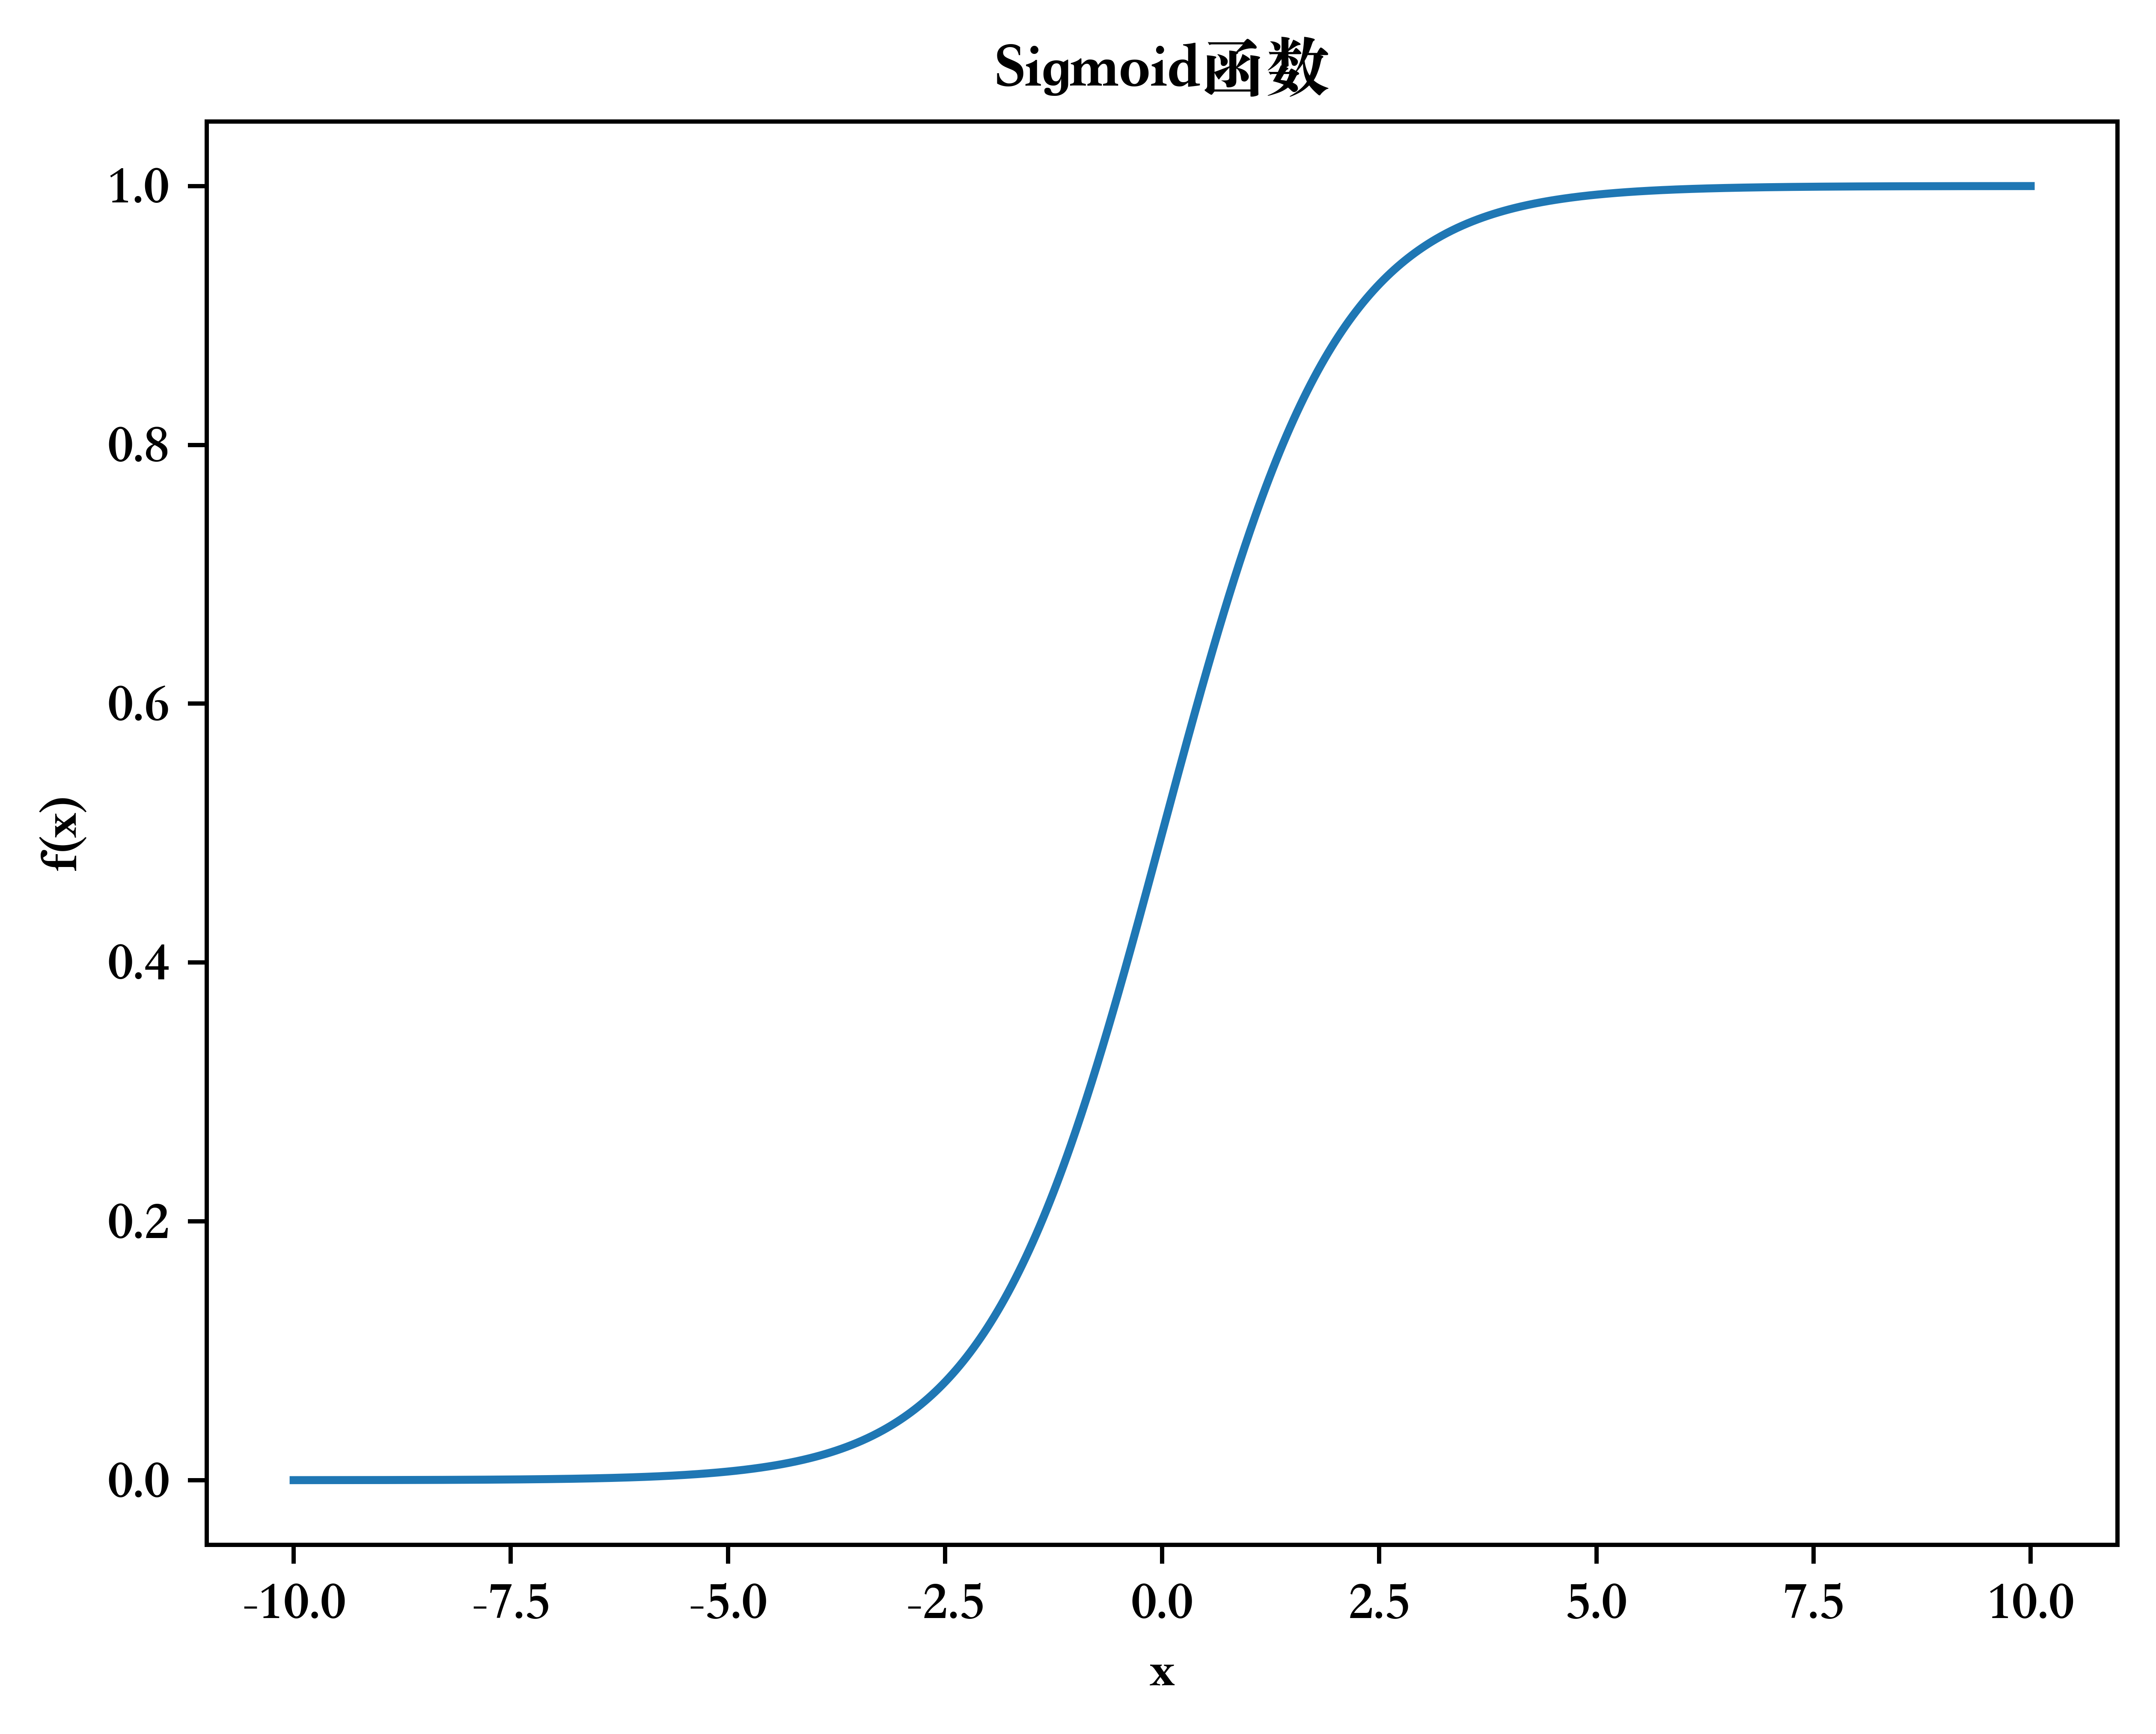
\includegraphics[width=.5\linewidth]{figures/content/sigmoid.png}
  \caption{Sigmoid函数图像}
  \label{Sigmoid}
\end{figure}


Sigmoid函数是可微的,这意味着它的导数可以在任何一点处计算出来,这使得它很适合用于反向传播,也就是用于训练神经网络的算法。此外,Sigmoid函数在0和1之间是有界的,这意味着它可以被解释为一个概率。然而,Sigmoid函数也有一些缺点。Sigmoid函数的主要问题之一是它存在梯度消失的问题。当Sigmoid函数的输入非常大或非常小时,函数的输出分别变得非常接近于0或1,函数的导数也会变得非常小,这可能导致梯度在反向传播期间消失。因为梯度在网络中向后传播时变得非常小,这样会使得网络难以学习更加深度的表征。


ReLU函数是神经网络中另一个常用的激活函数。它是一个片状线性函数,接受任何输入,如果输入是正的,就输出,否则就是0。ReLU函数的公式如下:

\begin{equation}
\label{eq:2_16}
f(x) = \max(0, x)
\end{equation}

ReLU函数图像如图\ref{ReLU}所示。
\begin{figure}[htbp]
  \centering
  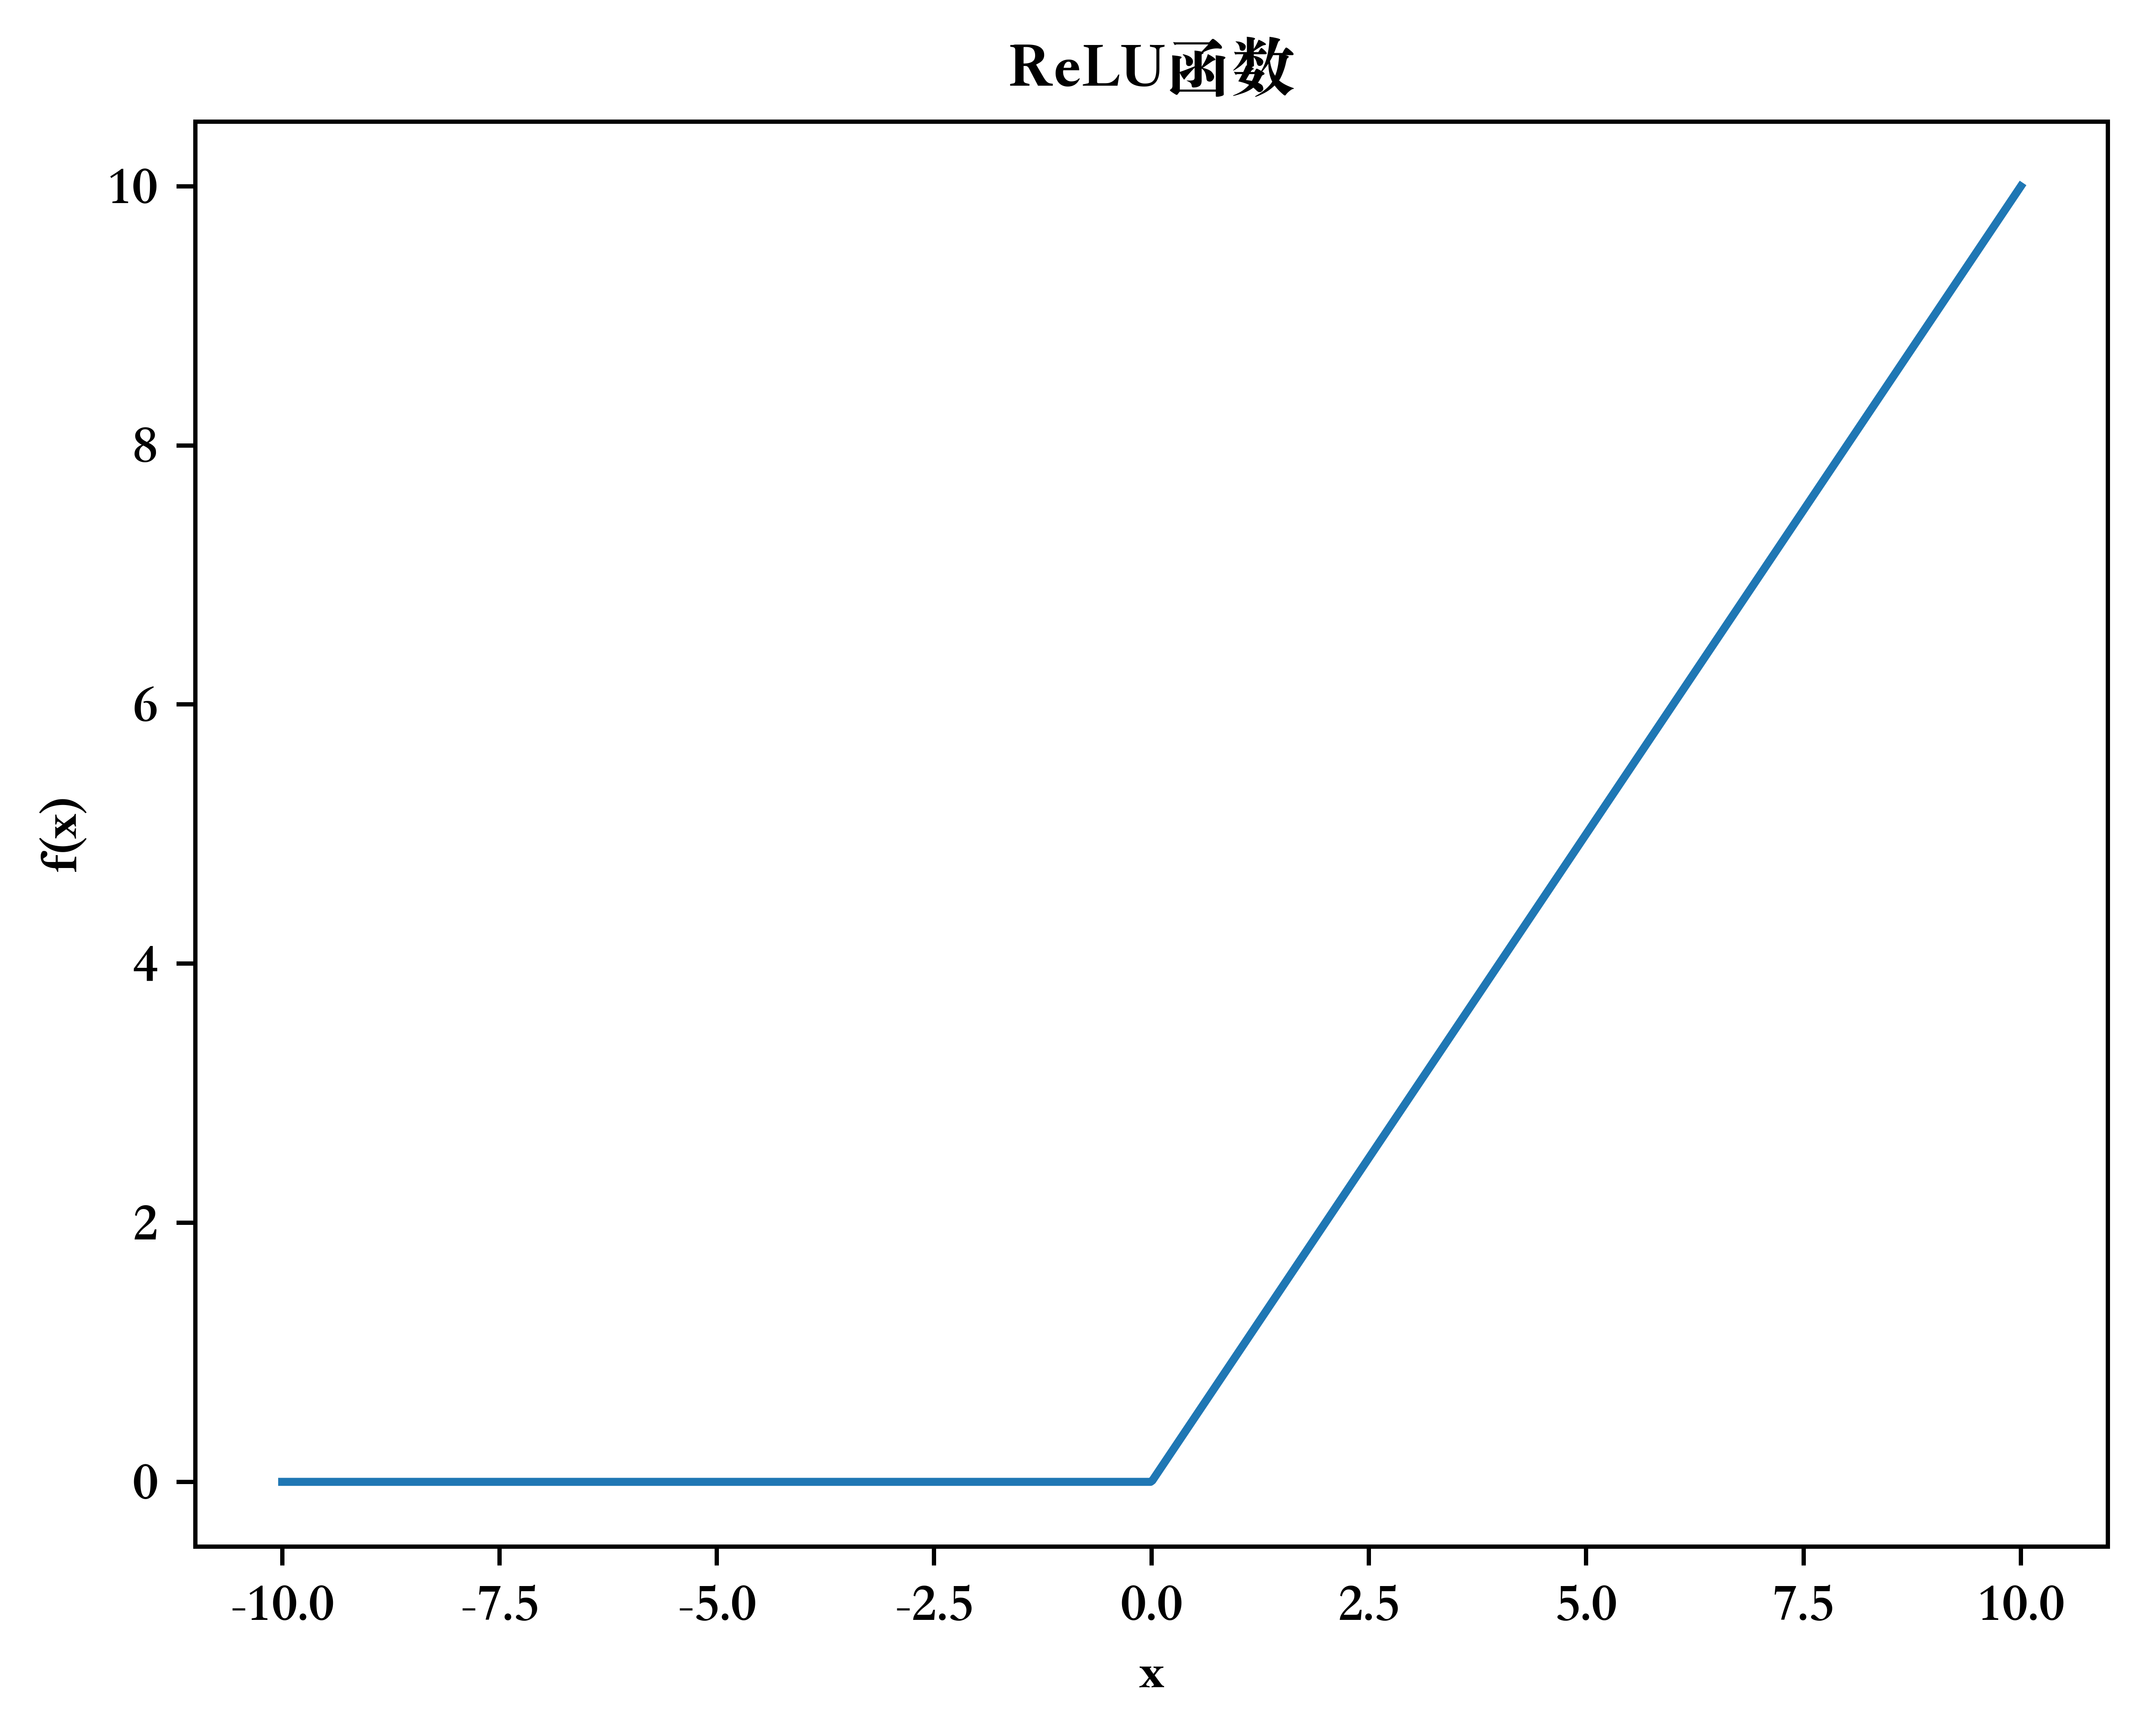
\includegraphics[width=.5\linewidth]{figures/content/ReLU.png}
  \caption{ReLU函数图像}
  \label{ReLU}
\end{figure}

ReLU函数的主要优点之一是它不存在梯度消失的问题。当ReLU函数的输入为正数时,该函数的导数为1,这意味着在反向传播过程中,其计算出的梯度仍然很大。因为梯度在通过网络向后传播时不会消失,这使得网络更容易学习深度表征。ReLU函数的另一个优点是它的计算效率高。由于该函数只是一个阈值操作,它可以用简单的逻辑运算来实现。然而,ReLU函数的一个主要问题是,当ReLU函数的输入为负数时,该函数的输出为0,这意味着神经元将会变得不活跃。这可能会导致整个神经元在训练过程中起不到任何作用,对网络的性能产生负面影响。


Softmax函数是一种特殊的激活函数,常用于进行分类任务的神经网络的输出层。Softmax函数的在接受到一个输入矢量后,会输出一个和为1的数值矢量,可解释为概率。Softmax函数图像如图\ref{Softmax}所示。

\begin{figure}[htbp]
  \centering
  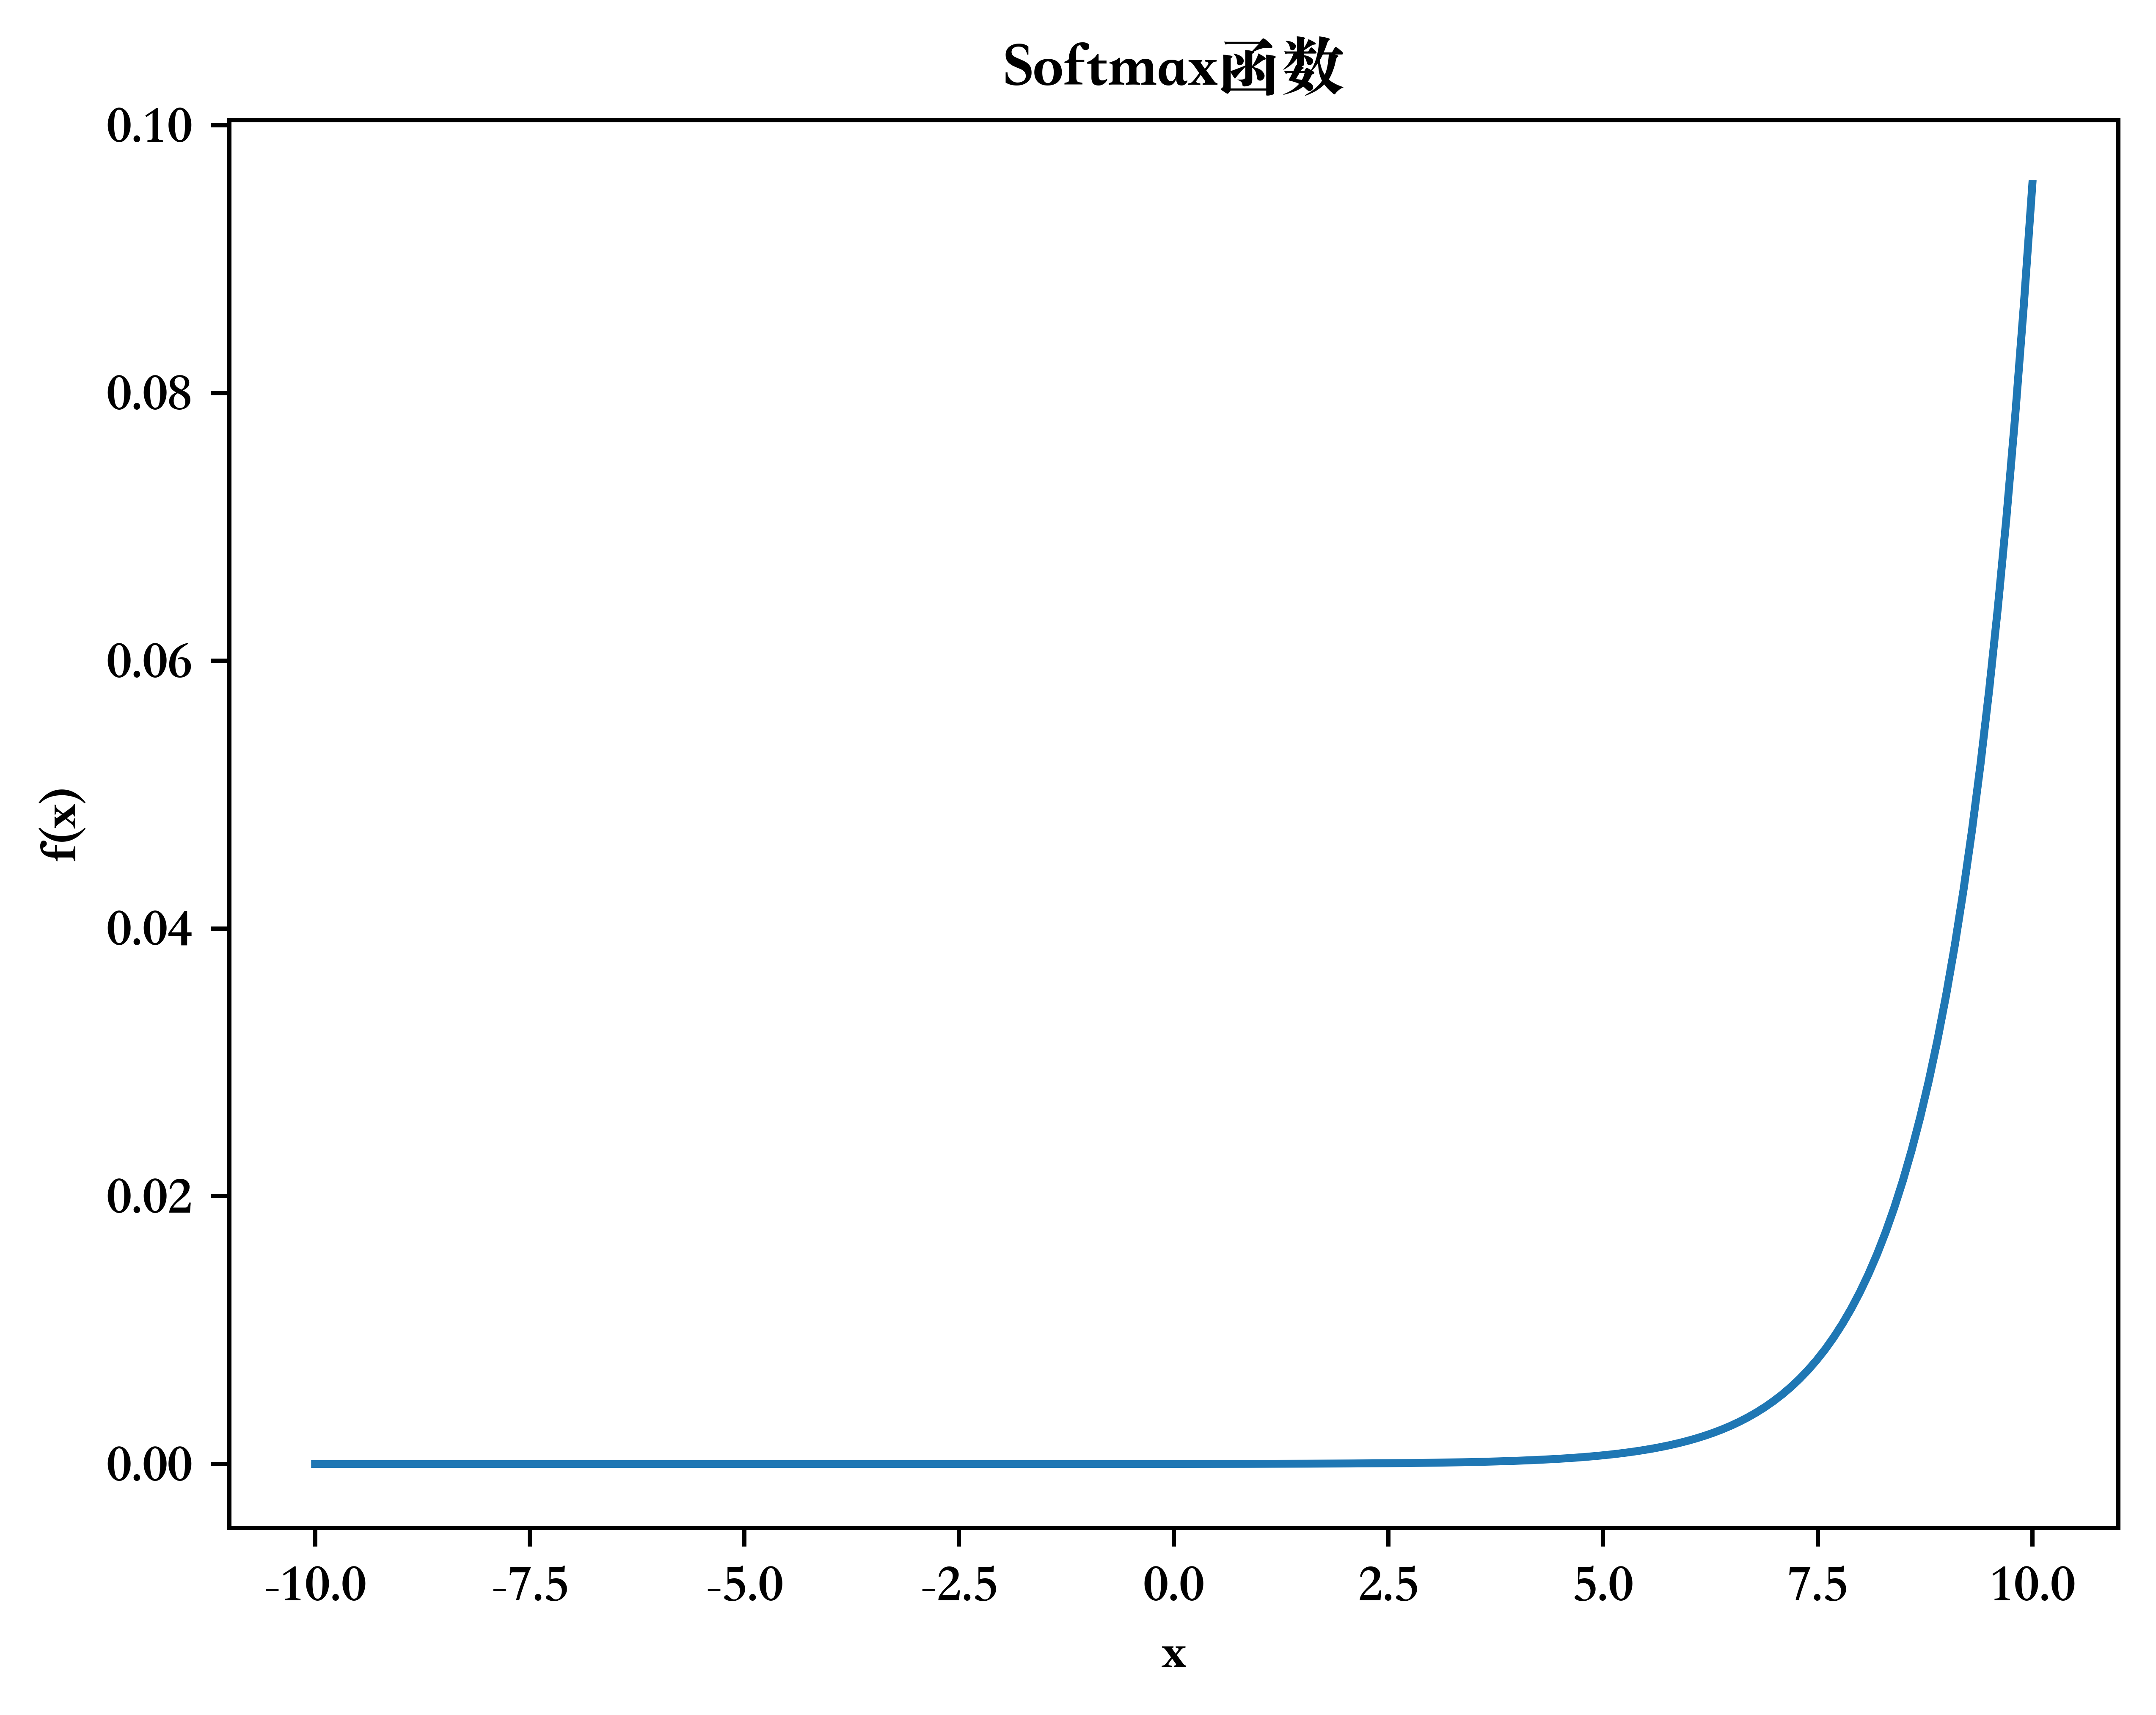
\includegraphics[width=.5\linewidth]{figures/content/Softmax.png}
  \caption{Softmax函数图像}
  \label{Softmax}
\end{figure}
Softmax函数由以下公式给出。
\begin{equation}
\label{eq:2_17}
f(x_i) = \frac{e^{x_i}} {\sum_{j}{e^{x_j}}}
\end{equation}

其中$x_i$是输入矢量的第$i$个元素,和是在矢量的所有元素上取的。

Softmax函数的主要优势是可以确保网络的输出被解释为概率。这使得它非常适合用于分类任务,其目标是将输入分配到几个可能的类别中的一个。此外,Softmax函数是可微分的,这意味着它可以用于反向传播来训练网络。

除了上面讨论的激活函数外,还有许多其他类型的激活函数被用于神经网络,包括双曲正切函数、指数线性单元(ELU)函数和缩放指数线性单元(SELU)函数等。这些激活函数都有自己的特性和使用场景,激活函数的选择取决于被解决的问题的具体需求,不同的激活函数可能更适合于不同类型的数据或任务。通过了解不同激活函数的特性,可以更好地设计神经网络,使其能够捕捉到实际数据中存在的复杂模式。


\subsection{损失函数及其优化算法}

损失函数是用来衡量神经网络的预测输出和实际输出之间差异的数学函数,其目标是提供一个衡量神经网络表现如何的标准。而损失函数优化是为了找到一组权重和偏置,使神经网络的预测输出与实际输出之间的差异最小。损失函数的选择取决于正在解决的具体问题。例如,对于回归问题,通常使用平均平方误差,而对于分类问题,通常使用交叉熵损失函数。

平均平方误差损失函数的公式如下:
\begin{equation}
\label{eq:2_18}
L = \frac{1}{n} \cdot \sum _i{y_i - \hat y_{i}}^2
\end{equation}

其中$n$是数据集中的样本数,$y_i$是第$i$个样本的实际输出,$\hat y_{i}$是第$i$个样本的预测输出,和是在数据集中的所有样本中取的。

交叉熵损失函数的公式如下:
\begin{equation}
\label{eq:2_19}
L = - \frac{1}{n} \cdot \sum _i{y_i \cdot \log{\hat y_i} + (1 - y_i) \cdot \log{(1 -\hat y_i})}
\end{equation}

其中$y_i$是第$i$个样本的实际输出(二元分类为0或1,多类分类为单次编码向量),$\hat y_i$是第$i$个样本的预测输出(0和1之间的概率),和是在数据集中的所有样本中取值。

神经网络最常用的优化算法是梯度下降法。梯度下降是一种迭代优化算法,它沿着损失函数的负梯度方向更新神经网络的权重和偏置。负梯度指向最陡峭的下降方向,这意味着沿着这个方向更新权重和偏置将导致损失函数值的减少。

梯度下降的更新规则如下:
\begin{equation}
\label{eq:2_20}
w_i = w_i - \alpha \cdot \frac{\mathrm{d}{L}}{\mathrm{d}{w_i}}
\end{equation}


其中$w_i$是第$i$个权重,$\alpha$是决定更新步长的超参数,$dL/dw_i$是损失函数相对于第$i$个权重的偏导。


随机梯度下降(SGD)是梯度下降的一个变种,它基于随机选择的小型训练数据子集来更新权重和偏差。这样做的好处是在计算上比梯度下降法更有效率,因为它只需要计算一小部分数据的梯度。随机梯度下降的更新规则与梯度下降相似,但使用在数据子集上计算的梯度而不是整个数据集,更新规则:
\begin{equation}
\label{eq:2_21}
w_i = w_i - \alpha \cdot \frac{\mathrm{d}{L_i}}{\mathrm{d}{w_i}}
\end{equation}

其中$\mathrm{d}{L_i} / \mathrm{d}{w_i}$是损失函数相对于当前数据子集的第$i$个权重的偏导。

总之,损失函数优化是深度学习的一个关键方面,因为它直接影响到神经网络的性能。通过使用各种优化算法,如梯度下降、SGD和Adam,我们可以训练我们的神经网络来最小化损失函数,并在各种任务中获得高精确度。


\section{深度强化学习}
\label{section:2.3}

深度强化学习是强化学习中应用深度学习的一种重要方法,可以解决一系列复杂的任务。本节将介绍深度强化学习中常用的算法包括深度Q网络、近端策略优化和深度确定性策略梯度等。深度Q网络是基于Q-learning算法的一种深度学习算法,可以直接学习环境状态和行为之间的映射关系,以实现最优策略的学习。近端策略优化是一种基于梯度的方法,用于直接优化策略函数,以提高强化学习模型的性能。深度确定性策略梯度则是将近端策略优化与确定性策略相结合,以实现高效的连续动作控制。本节将深入探讨这些深度强化学习算法的原理和应用。

\subsection{深度Q网络}

深度Q网络(DQN)是基于Q-learning算法的深度强化学习算法,其目的是使用深度神经网络来近似给定状态-动作对的最佳动作价值函数。在Q-learning中,智能体通过选择最大化动作价值Q的行动来学习最大化其预期的未来回报,Q值是在给定状态下采取行动并在之后遵循给定策略的预期未来回报。

在式\ref{eq:2_2}和式\ref{eq:2_3}中分别给出了动作价值和最佳动作价值的定义,DQN算法使用一个深度神经网络来近似动作价值函数。该神经网络将当前状态作为输入,为每个可能的行动输出一个动作价值,智能体所选动作的动作价值被用来更新神经网络的权重。在DQN算法中,下一个状态的动作价值是用目标网络来估计的,目标网络是一个具有固定权重的主网络的复制模型。目标Q值被用来更新主网络的权重,主网络被用来估计当前状态的动作价值。DQN中使用的平均平方误差损失函数,它用于衡量网络输出的Q值和目标Q值之间的差距。可根据式\ref{eq:2_18}得到用于更新神经网络权重的损失函数$L(\theta)$:
\begin{equation}
\label{eq:2_22}
L(\theta) = E\left[\left(r + \gamma \cdot \max _{a'} Q(s', a', \theta') - Q(s, a, \theta)\right)^2\right ]
\end{equation}


其中,$\theta$是主网络的权重,$\theta '$是目标网络的权重,$r$是在状态$s$下采取行动$a$后获得的即时奖励。

DQN算法使用经验回放来提高学习效率和稳定性。经验回放存储了一个固定大小的经验缓冲区,神经网络通过从缓冲区中随机抽取经验进行训练。经验重放减少了连续经验之间的相关性,使学习过程更加有效。经验重放也有助于防止网络对最近的经验过度拟合。

DQN算法使用epsilon-greedy探索来平衡对新行动的探索和对当前策略的利用。Epsilon-greedy探索以1-$\epsilon$的概率选择具有最高Q值的行动,以$\epsilon$的概率选择一个随机行动。

\begin{equation}
\label{eq:2_23}
{a}_{t}= \begin{cases}\underset{{a} \in A}{\operatorname{argmax}} Q\left({s}_{t} ,{a}\right) & \text { 当概率为 } 1-\varepsilon, \\ \operatorname{rand}({a}) & \text { 当概率为 } \varepsilon.\end{cases}
\end{equation}


总之,DQN算法是一种被广泛使用的强化学习方法,用于训练强化学习问题中的动作价值函数。它通过使用神经网络来近似动作价值函数,解决了传统Q-learning算法的一些局限性,这使得它可以在类似的状态和行动中进行泛化。它还使用了一个经验重放缓冲器和一个目标网络来提高稳定性并防止过度拟合。DQN算法已被成功应用于各种具有挑战性的决策问题中,包括游戏、机器人的控制等。


\subsection{近端策略优化}

近端策略优化(PPO)是一种近年来备受关注的深度强化学习策略优化算法,属于策略梯度方法,这意味着它将从当前策略收集的经验中学习。PPO算法的基本原理是通过优化策略函数来寻找最优策略。通过式\ref{eq:2_7}可以得知,在强化学习中,策略函数$\pi(a \mid s)$通常是一个映射函数,它将当前状态作为输入,输出对应的行动。PPO算法通过反复迭代,不断更新策略函数,使其逐渐趋于最优。

该算法的核心思想是限制每次策略更新的大小,避免策略函数发生大幅度变化,导致训练不稳定。具体而言,PPO算法采用一种被称为“近端策略优化”的方法,通过在优化目标函数中增加一个约束项来限制每次策略更新的大小,这个约束项通常被称为“剪切项”,它会限制新旧策略之间的差异,并确保每次策略更新的大小不超过一个预设的阈值,以确保优化的稳定性。在PPO算法中,优化目标函数是最大化经过剪切后的期望优势函数,而不是最大化期望回报函数。这里的优势函数表示当前策略相对于旧策略的性能提升程度。在PPO算法中,我们使用剪切方法来限制当前策略和旧策略之间的差异,其优化目标函数可以写作:

\begin{equation}
\label{eq:2_24}
L_{\text{CLIP}}(\theta) = \mathbb{E}_t\left[\min\left(\frac{\pi_{\theta}(a_t|s_t)}{\pi_{\theta_{\text{old}}}(a_t|s_t)}A_t, \text{clip}\left(\frac{\pi_{\theta}(a_t|s_t)}{\pi_{\theta_{\text{old}}}(a_t|s_t)}, 1-\epsilon, 1+\epsilon\right)A_t\right)\right]
\end{equation}

其中,$\theta$表示当前策略的参数,$\theta_{\text{old}}$表示旧策略的参数,$\pi_{\theta}(a_t|s_t)$表示在状态$s_t$下,当前策略选择动作$a_t$的概率,$\pi_{\theta_{\text{old}}}(a_t|s_t)$表示在状态$s_t$下,旧策略选择动作$a_t$的概率,$A_t$表示在时刻$t$的优势函数,用于表示在给定状态 $s_t$ 和行动 $a_t$ 下,相比于平均水平的预期奖励,当前策略的表现优劣程度。具体地,$A_t$ 的定义如下:
\begin{equation}
\label{eq:2_25}
A_t = Q(s_t, a_t) - V(s_t)
\end{equation}

式\ref{eq:2_24}中,目标函数$L_{\text{CLIP}}(\theta)$的第一项表示策略更新的目标是最大化期望回报函数,第二项表示对策略更新进行剪切,确保新策略不会偏离原来的分布太远。通常来说,$\epsilon$的取值较小,可以取$0.1$或$0.2$等较小的数值。当$\epsilon$取较小值时,第二项的影响较小,策略更新更倾向于最大化期望回报函数。

在PPO算法中,更新价值函数的方法通常是通过均方误差(MSE)损失函数来实现,类似于式\ref{eq:2_22}。PPO算法已经在多个实际应用场景中得到了广泛的应用,然而,PPO算法也存在一些不足之处。例如,PPO算法对于大规模离散动作空间的问题处理较为困难,同时其算法复杂度较高,需要消耗大量的计算资源。此外,PPO算法在处理一些特殊场景下,如存在不确定性的环境、存在噪声的环境等,可能会出现训练不稳定的问题。


\subsection{深度确定性策略梯度}

深度确定性策略梯度(DDPG)算法是一种结合了深度神经网络和确定性策略梯度的强化学习算法,主要用于解决连续动作空间的问题,这类问题中,智能体需要在一个连续的动作空间中选择动作,因此传统的强化学习算法无法直接应用于该类问题。DDPG算法通过结合深度神经网络和确定性策略梯度的方法,解决了这一问题。与传统的Q-Learning算法相比,DDPG算法在处理连续动作空间问题时,可以直接输出动作值,而无需在离散动作空间中搜索最优动作。

DDPG算法的主要思路是通过Actor-Critic模型来学习动作值函数,同时通过确定性策略梯度的方法来更新策略函数。其主要由四个部分组成:策略网络、价值网络、经验回放缓存和目标网络。其中策略网络和价值网络都采用深度神经网络来进行参数化,在训练时首先需要通过经验回放缓存来收集一定数量的状态转移样本,然后从中随机采样一批样本,用于网络的训练。策略网络的作用是输出在当前状态下最优的动作值。价值网络的作用是评估策略网络输出该动作值优劣的评估值,然后根据这个评估值计算出相应的策略梯度,最后通过反向传播算法更新策略网络的参数。经验回放缓存的作用是记录智能体在环境中的经验,并从中随机采样用于网络的训练。目标网络的作用是解决训练不稳定的问题,其参数是由价值网络参数每隔一段时间拷贝而来的。


DDPG算法的主要优点可以总结为以下几个方面。首先,DDPG算法采用Actor-Critic模型,可以直接输出动作值,因此可以直接处理连续动作空间问题。其次,DDPG算法引入目标网络和经验回放缓存技术,可以提高网络的训练稳定性。此外,DDPG算法使用深度神经网络处理高维状态空间问题,可以有效提取状态特征信息,提高智能体的决策效果。最后,DDPG算法结合了确定性策略梯度和Q-Learning的思想,可以同时处理具有连续动作空间和延迟奖励的问题。

然而,DDPG算法也存在一些缺点:1.使用经验回放缓存和目标网络等技术来提高训练的稳定性的同时会导致了训练时间的增加。2.DDPG算法有许多超参数需要调节,例如网络结构、学习率、优化器等,这些超参数的不同取值会影响算法的表现,参数调节较为复杂。3.DDPG算法在处理连续动作空间问题时,通常需要引入噪声,但对噪声的选择和调节会对算法的表现产生较大影响,对噪声较为敏感。

\subsection{深度强化学习算法的对比与选择}

在解决出行模式和时间选择问题时,本章已经介绍了三种深度强化学习算法:深度Q网络、近端策略优化和深度确定性策略梯度。现在需要对这三种算法进行对比,并最终在出行模式与时间选择的场景下适用的方法。

DQN算法是一种基于Q-Learning算法和深度神经网络的强化学习算法。其优点是训练速度快、稳定性高,而且适用于离散动作空间和连续动作空间。缺点是难以处理连续状态空间问题。

PPO算法是一种基于策略梯度的强化学习算法。其优点是能够处理连续状态空间和连续动作空间问题,具有很好的表现。缺点是训练速度较慢,而且需要大量的超参数调节。在解决出行模式和时间选择问题中,我们的状态空间较大,因此DQN算法的表现可能会受到限制。


DDPG算法是一种基于Actor-Critic模型和深度神经网络的强化学习算法。其优点是能够直接处理连续动作空间问题和高维状态空间问题,而且能够处理具有延迟奖励的问题。缺点是训练时间较长,且对超参数的调节比较敏感。

表\ref{tab:2_1}总结并列出了三种算法的优缺点。

\renewcommand{\arraystretch}{1.5} % 使表格行间距加大1.5倍
\begin{table}[htbp]
\centering
\caption{三种深度强化学习算法的对比}
\label{tab:2_1}
\begin{tabular}{cll}
\toprule
模型 & \multicolumn{1}{c}{优点}       & \multicolumn{1}{c}{缺点}     \\
\midrule
深度Q网络                       & \parbox[t]{5.5cm}{训练速度快,稳定性高,可以处理高维状态空间和延迟奖励}      & \parbox[t]{5.5cm}{只适用于离散动作空间,对参数的选择比较敏感 }                       \\
近端策略优化                       & \parbox[t]{5.5cm}{收敛速度快,能够保持高样本效率}    & \parbox[t]{5.5cm}{训练时间较长,需要手动调整超参数}              \\ 
深度确定性策略梯度                    & \parbox[t]{5.5cm}{处理高维状态空间和延迟奖励,学习到高质量的策略}   & \parbox[t]{5.5cm}{对参数的选择比较敏感,难以处理高维状态空间}              \\
\bottomrule
\end{tabular}
\end{table}



因为问题的场景是一个离散的动作空间,而且DQN算法的训练速度快、稳定性高,适合处理这种场景。同时,考虑到算法的可解释性和易于实现性,DQN算法在这方面也具有优势。虽然近端策略优化算法在处理连续状态空间和连续动作空间问题上表现较好,但在本文的问题中,状态空间较大,训练速度也较慢,不太适合。深度确定性策略梯度算法可以处理连续动作空间和高维状态空间问题,但运算时间成本较高,且对超参数的调节比较敏感,因此也不太适合处理本文的问题。因此,综上所述,针对出行模式和时间选择问题,通过对三种主流的深度强化学习算法的优缺点分析,最终选择深度Q网络算法作为本文解决问题的主要深度强化学习方法。

\section{本章小结}

本章主要介绍了深度强化学习相关的知识和技术。在\ref{section:2.1}小节中首先详细介绍了强化学习中的相关术语,包括智能体、状态、动作、策略、奖励、回报以及状态转移等,这些概念是深度强化学习算法的基础。随后,依据智能体选择策略的原理梳理了基于价值、基于策略以及基于价值和策略相结合的强化学习方法。这些方法各有特点和优缺点。基于价值的方法主要学习状态值函数或状态动作值函数,而基于策略的方法则直接学习策略函数。基于价值和策略相结合的方法则既学习状态值函数又学习策略函数。在实际应用中,我们需要根据问题的具体特点选择合适的方法来解决问题,以获得最佳的效果。介绍深度强化学习之前,在\ref{section:2.2}小节简要介绍了深度学习的基本知识,包括神经网络、激活函数以及损失函数和优化算法等。这些知识对于理解深度强化学习算法是非常重要的。之后,在\ref{section:2.3}小节详细介绍了三种深度强化学习算法中常用的方法,包括深度Q网络、近端策略优化、深度确定性策略梯度。这些方法使用深度神经网络来近似值函数或策略函数,使得智能体可以在高维状态空间中进行学习和决策。最后,通过对比了不同深度强化学习算法的优缺点,选择了深度Q网络的方法作为研究出行模式和时间选择的主要方法。      % 第二章:
\chapter{仿真实验场景的设计与构建}

\section{城市交通仿真平台的可行性分析}

\subsection{Vissim介绍}

VISSIM(VISual SIMulation)是由德国PTV(Planung Transport Verkehr AG)公司开发的一款功能强大的交通模拟软件。它被广泛应用于交通规划、设计、管理等领域。VISSIM可以模拟各种复杂的交通场景,包括城市道路、高速公路、交叉口、公共交通,以及交通流、交通信号控制、公共交通路线规划、车辆路径规划等。
VISSIM的基本功能包括:

1.建模。VISSIM的建模功能非常强大。用户可以使用VISSIM的图形用户界面轻松创建交通场景,如道路、交叉口和公共交通路线。用户还可以调整交通流率、车辆类型、行人流量和其他参数,以建立一个交通网络。在VISSIM的智能交通生成器的帮助下,可以快速、准确地创建交通场景。交通生成器使用真实的交通数据,为一天中的不同时段、工作日和周末创建真实的交通流模式。交通生成器还允许用户定制交通情景,并调整交通量、速度和其他参数。

2.仿真模拟。VISSIM提供了一个高保真的交通仿真引擎,可以高度准确地模拟各种交通场景。用户可以运行各种交通管理策略的模拟,如交通信号控制、公共交通路线规划和车辆路径规划。仿真引擎还可以生成实时交通数据,如车辆速度、行驶时间和延迟时间。有了这些数据,用户可以评估不同交通管理策略的性能,比较不同的方案,并做出明智的决定。

3.分析功能。VISSIM提供了一个强大的分析功能,使用户能够分析和可视化模拟结果。用户可以生成大量的图表和表格来分析交通流量、拥堵情况、车辆行驶时间、车辆速度和其他指标。分析功能还允许用户比较不同交通管理策略的性能,评估不同参数对交通流的影响。

VISSIM是一个全面而强大的交通模拟软件,为用户提供准确而真实的模拟结果。该软件支持各种类型的交通场景,从小型交叉口到大型城市网络。建模功能允许用户创建一个虚拟的交通网络,模拟引擎产生的实时交通数据可用于评估不同的交通管理策略和交通计划。该软件的高级功能,如定制、多模式模拟、行人模拟、排放和油耗以及驾驶辅助系统,为用户提供了一套全面的工具来评估交通网络的性能和影响。总之,VISSIM是交通专业人员、研究人员和政策制定者设计、分析和优化交通系统的重要工具,以实现更安全、更高效和可持续的未来。


\subsection{SUMO介绍}

SUMO(Simulation of Urban Mobility)是一款开源的交通仿真软件,被广泛应用于城市交通规划、交通管理、交通研究等领域。SUMO是由德国科研机构DLR开发,其设计目标是实现高效、可扩展和高度自定义的交通仿真,同时提供良好的可视化和数据输出。SUMO具有开放性、高可靠性、高可扩展性和良好的可视化效果等特点,成为了交通仿真领域的重要工具之一。

SUMO的基本功能包括:

1.建模。SUMO提供了强大的建模功能,允许用户创建一个虚拟交通网络。该软件支持各种道路网络,包括高速公路、公路、交叉口和环岛等。用户可以定义网络中的道路布局、交通流和车辆类型。此外,该软件还提供了从各种文件格式(如OpenStreetMap)导入道路网络的工具。

2.仿真技术。SUMO使用微观交通模拟引擎,提供准确和真实的模拟结果。该软件可以模拟各种交通场景,如车辆路线、公共交通和行人运动。仿真引擎能够生成实时交通数据,如旅行时间、车辆速度和延迟时间。这些数据可以用来评估不同的交通管理策略和交通计划。

3.可视化。SUMO提供了一个用户友好的图形用户界面,允许用户对模拟结果进行可视化。该界面提供了一个交通网络的实时视图,并可以显示个别车辆、行人和公共交通的运动。此外,该软件还提供了生成各种图表和表格的工具,以总结模拟结果。

SUMO的高级功能有:

1.定制功能。SUMO是高度可定制的,允许用户定义影响模拟的不同参数,如车辆类型、司机行为和交通信号。该软件还提供了一个脚本接口,允许用户通过编写自定义脚本来扩展软件的功能。用户还可以创建自定义的车辆模型,并将其导入到模拟中。

2.多模式仿真。SUMO支持多模式模拟,允许用户模拟多种交通方式,如汽车、公交车、火车和自行车。这个功能可以评估不同交通方式的性能,并对不同的交通计划进行比较。

3.优化功能。SUMO提供优化功能,使用户能够改善交通网络的性能。该软件可以优化交通信号灯时间、车辆路线和公共交通时间表。优化功能允许用户找到最佳的交通管理策略和交通计划。

4.并行化。SUMO提供并行化功能,允许用户在多个处理器上运行模拟。这个功能加快了模拟时间,并能模拟更大的交通网络。

5.集成。SUMO可以与其他软件工具集成,如交通流模型、地理信息系统(GIS)和数据分析工具。集成功能使数据的交换和定制解决方案的开发成为可能。

总之,SUMO是一个功能强大、用途广泛的模拟软件,为用户提供了一套全面的工具来模拟和分析各种交通情况。该软件支持多模式交通的模拟,包括汽车、公交车、自行车和行人,它还提供了一些高级功能,如交通需求生成、交通信号控制和车辆路由。SUMO的灵活架构和开源代码库使其成为研究人员、交通专业人士和需要高度可定制模拟工具的决策者的热门选择。SUMO有能力生成真实的交通数据,并提供对交通系统性能的洞察力,在设计、优化和评估交通系统方面发挥了关键作用,以实现更安全、更高效和可持续的未来。

\subsection{Matsim介绍}

MATSim是一个开源的、基于代理的、多模式的交通模拟软件,为城市或地区的个人行为和整个交通系统的建模和模拟提供了一个平台。该软件由瑞士苏黎世联邦理工学院(ETH Zurich)的一个研究团队历经数年开发,目前已被世界各地的研究人员、交通规划人员和政策制定者广泛使用。

MATSim提供了一套全面的功能来模拟和仿真不同的交通场景。它将个人旅行者建模为代理人,根据他们的偏好和现有的交通选择做出决定。代理人可以选择不同的交通方式,如汽车、公共交通、步行或骑自行车,他们还可以选择最短、最快或最舒适的路线来到达目的地。该软件的先进模拟引擎可以生成大规模的模拟,可以在任何标准计算机系统上运行。

MATSim软件基于模块化架构,允许用户根据自己的具体需求定制软件。这些模块可以被扩展或被其他模块取代,以模拟新的运输系统或包括新的功能。这一特点使该软件能够适应不同交通场景的具体要求,并使其成为研究人员和交通专业人士的热门选择。

MATSim的主要特点之一是它能够模拟多模式的交通系统。它可以模拟广泛的交通选择,包括汽车、公共汽车、火车、自行车和步行,并且可以模拟不同交通方式之间的相互作用。这使用户能够评估不同交通系统的性能,并优化城市或区域内不同交通方式的使用。

MATSim还包括一个全面的可视化工具,允许用户实时查看模拟的结果。该软件的可视化模块使用户能够看到模拟的代理人在交通网络中移动,做出决定,并到达他们的目的地。可视化模块还可以显示模拟的交通流量、旅行时间和其他重要指标,可用于评估交通系统的性能。

MATSim的另一个主要特点是其开源代码库。该软件是在GNU通用公共许可证下发布的,它允许用户修改软件并将其分发给其他人。这一特点使研究人员和交通专业人士能够合作和分享他们的工作,使MATSim成为交通规划和管理领域的研究和开发项目的热门选择。

此外,MATSim软件已经由一个研究人员和交通专业人士团队进行了广泛的测试和验证。该软件已被用于对全球不同城市和地区的交通系统进行建模和模拟,包括苏黎世、柏林、悉尼、新加坡等。这有助于建立该软件的可信度和可靠性,并证明其对交通系统进行精确建模和模拟的能力。

总之,MATSim是一款功能强大、用途广泛的交通仿真软件,为用户提供了一套全面的工具来模拟和仿真不同的交通场景。该软件的模块化架构、多模式模拟能力、先进的可视化功能和开源代码库使其成为研究人员和交通专业人士的热门选择。MATSim能够准确地模拟交通系统并评估不同交通方案的性能,在设计、优化和评估交通系统以实现更安全、更高效和可持续的未来方面发挥了关键作用。


\subsection{仿真平台的选择}

在这三个交通模拟软件中,我会选择SUMO,原因有很多。

首先,SUMO是一个开源软件,这意味着它可以免费下载和使用。这对于预算紧张的人来说是一个很大的优势,因为使用SUMO没有任何许可费用。此外,SUMO的开源性质意味着它是高度可定制的,这使得用户可以根据他们的具体需求来修改软件。

其次,SUMO是一个高度通用的软件,可以模拟多模式的交通场景。它可以模拟汽车、公共汽车、自行车、行人,甚至火车。这意味着用户可以对各种交通场景进行建模和模拟,并评估不同交通方案的性能。

第三,SUMO是一个高度精确的模拟软件。该软件以先进的交通流和车辆动力学模型为基础,提供高度真实和准确的结果。这使得SUMO成为交通专业人士、研究人员和政策制定者的重要工具,他们需要评估交通系统的性能,并优化它们,以实现更安全、更高效和可持续的未来。

第四,SUMO有一个友好的界面,这使得初学者和高级用户都很容易使用。该软件的界面允许用户创建和修改交通网络,生成交通需求,并评估不同交通系统的性能。SUMO还提供了一套全面的可视化工具,使用户可以实时查看模拟结果。

第五,SUMO有一个庞大而活跃的用户社区,它提供了丰富的资源,包括教程、文档和用户论坛。这意味着,如果用户在使用该软件时遇到任何问题,可以很容易地找到支持和帮助。此外,用户社区还提供了一个合作和分享最佳实践和新发展的平台。

最后,SUMO是交通行业中备受推崇和广泛使用的交通仿真软件。它已被用于模拟和仿真世界上许多城市和地区的交通系统,包括欧洲、亚洲和北美。这意味着SUMO已经被交通专业人员广泛测试和验证,其结果也被政策制定者和决策者所信任。

总之,SUMO是一个强大的、多功能的交通仿真软件,为用户提供了一套全面的工具来模拟和仿真不同的交通场景。它的开源性、多模式模拟能力、准确性、用户友好的界面、活跃的用户社区和受人尊敬的声誉使它成为交通专业人士、研究人员和决策者的热门选择。凭借其准确模拟交通系统和评估不同交通方案性能的能力,SUMO在设计、优化和评估交通系统以实现更安全、更高效和可持续发展的未来方面发挥了关键作用。

\section{基于SUMO的城市交通仿真平台}

\subsection{平台设计目标}
 

\subsection{功能模块简介}

\section{实验场景的选择与搭建}

\subsection{路网的编辑与生成}

\subsection{出行模式的设计}

\subsection{流量的生成}      % 第三章:
\chapter{基于深度强化学习的出行模式与时间选择方法}
\label{chp:float}

强化学习是一种通过迭代地改进策略来最大化累计奖励或回报的机器学习方法。在应用强化学习到具有马尔可夫属性的序列决策过程中,需要先构建一个马尔可夫决策过程,该过程定义了环境的演变,考虑到强化学习代理所采取的行动。强化学习代理通过行动探索和开发不断地与环境互动,根据当前状态 $s_t$ 进行行动。每次行动会使环境演变成一个新状态 $s_{t+1}$,并获得相应的奖励 $r_t$,反馈给代理以改善其决策逻辑。这个过程一直迭代,直到代理成功学习到一个能够最大化累计奖励的策略 $\pi$,也就是一个决策者。因此,强化学习的关键在于根据奖励不断迭代改进策略。

在本研究中,将每个出行者视为具有学习能力的智能实体,通过马尔可夫决策过程来建模每个出行者跨越多个连续日的交通出行行为。每个出行者能够选择的行动包括不同组合的出行方式和出发时间。最终由个人采取的行动 $a_t$ 决定了环境演变到的下一个状态 $s_{t+1}$。该状态应反映个人关于行程本身以及相关环境的最新知识。选择此行动所获得的奖励 $r_t$(与旅行成本相关)有助于改善个人的决策逻辑,这样个人就能逐渐学习到最优的行动策略,并最大化累计奖励。
\section{马尔可夫决策过程框架}
正如先前所讨论的那样,马尔可夫决策决策过程是建模和优化出行模式和时间选择的先决条件。从数学角度来说,它是一个五元组$(S, A, P, R, \gamma)$,其中$S$表示状态空间,$A$表示动作空间,$P$表示状态转移概率,$R$表示奖励函数,最后$\gamma$是折扣因子。在这里,智能体是出行模式和时间选择中个人的决策者。虽然将每个个体视为智能体在概念上是有效的,但是由于代理数量等于个体数量,所产生的计算复杂性是大规模应用的主要障碍。从推荐系统的角度来看,研究适用于所有个体的常见决策逻辑是值得探究的,这反映了该方法的普适性。接下来,我们将进一步阐述如何构建和解决问题特定的马尔可夫决策决策过程。

\subsection{动作空间}

动作空间是强化学习中的一个关键概念。在建模动作空间时需考虑出行者的个性化特征。例如,不同出行者对于出行方式和出发时间的偏好不同,因此他们的动作空间也会不同。对此,可以引入个性化因素对动作空间进行建模。例如,可以考虑出行者的年龄、性别、职业、家庭状况等因素,进一步细化动作空间的描述,提高模型的预测能力和适应性。

此外,动作空间的大小和粒度也会影响到模型的性能和可解释性。如果动作空间过大,模型的训练和预测会变得非常困难,同时也会增加模型的计算复杂度和存储空间需求。而如果动作空间过小,模型的表达能力就会受到限制,无法对真实情况进行有效建模。因此,需要在合理范围内对动作空间进行定义和限制,以平衡模型的性能和可解释性。在实际应用中,建模动作空间的过程也需要考虑到数据的可用性和质量。例如,在收集出行调查数据时,需要尽可能全面和准确地收集出行者的出行方式和出发时间等信息,以便更好地建模动作空间和进行模型预测。同时,在对数据进行预处理和清洗时,也需要对动作空间进行适当的定义和筛选,以避免噪声和异常数据对模型的影响。

在JTMDTC中,动作空间包括出行方式和出发时间两个方面。在选择出发时间时,出行者需要考虑到交通拥堵、出行时间和其他因素对行程的影响。例如,在高峰期出发可能需要更长的旅行时间,而在非高峰期出发可能可以更快地到达目的地。因此,在建模动作空间时,需要综合考虑各种因素,以便在代理决策时提供准确的信息。出行方式可以是私家车、公共交通或自行车。在公共交通中,可以选择乘坐公交车或地铁,但是不考虑三种交通方式之间的换乘。这是因为换乘涉及到很多变量,比如停车地点、换乘时间等,需要更多的研究来处理。

对于出发时间,每个出行者都有一个初始或期望出发时间$t_0$。但是,由于各种原因,可能需要调整出发时间,比如交通拥堵、天气等。在JTMDTC中,出发时间可以在一个时间窗口$[t_{\min},t_{\max}]$内进行调整。这个时间窗口是由最早和最晚的出发时间$t_{\min}$和$t_{\max}$确定的。出发时间的调整是以离散间隔为单位进行的,而不是连续方式进行。这是因为在实际交通中,时间通常是以分钟为单位进行的,而不是连续的时间。

对于上述所提到的交通方式和出发时间,需要进行适当的编码以便于代理在模型中进行操作。在本文中,采用离散化编码的方式,将交通方式和出发时间分别离散化为一组离散的选项。例如,对于交通方式,可以将私家车、公交车、地铁和自行车分别编码为$m_1$、$m_2$、$m_3$和$m_4$。对于出发时间,可以将$t_0$和时间窗口$[t_{\min},t_{\max}]$离散化为一组时间步长,例如每5分钟一步。这样,代理可以从一组离散的选项中进行选择,并决定最佳的出行方式和出发时间。动作空间的描述采用了向量的形式。向量$\bm{a}$包括交通方式$\tilde{m}$和出发时间$\tilde{t}$。交通方式可以是可用交通方式$m_{1},m_{2}, \ldots, m_{N}$中的任意一种,而出发时间必须在时间窗口$[t_{\min }, t_{\max }]$内。因此,动作空间可以表示为:
\begin{equation}
\bm{a}=\left[\begin{array}{c}
\tilde{m} \\
\tilde{t}
\end{array}\right]=\left[\begin{array}{c}
\text { 出行模式 } \\
\text { 出发时间 }
\end{array}\right]
\in\left[\begin{array}{c}
\left\{m_{1},m_{2}, \ldots, m_{N}\right\} \\
{\left[t_{\min }, t_{\max }\right]}
\end{array}\right],
\end{equation}


动作空间是模型中重要的一部分,它定义了代理能够采取的所有行动,直接影响着模型的效果和性能。在建模时,需要综合考虑多种因素,将交通方式和出发时间等重要信息进行适当的编码,以便于代理进行决策。
\subsection{状态空间}

状态空间定义了智能体选择行动的上下文环境。对于JTMDTC,状态空间被设计为不仅包含有关行程的最新知识,还包括智能体早期经验。这种状态空间设计在很大程度上类似于理性人类的决策机制,即从经验中学习。由于重点不在于经验选择建模而在于选择指导或推荐,因此我们假设智能体能够充分感知环境,因此对行程具有完全信息。然而,我们稍后将讨论这种假设可能会有所放松。

行程信息首先包括每种交通方式的旅行距离$L$和记忆旅行时间$\bar{T}$。前者是模式$m$的旅行距离,而后者是模式$m$的平均经验旅行时间。其原因有两个——利用经验和在交通随机性存在的情况下保持稳健性。作为行程信息的另外两个变量是初始出发时间$t_0$和出发时间差或偏移量$\Delta t$相对于$t_0$。将所有内容组合起来,得到以下特定于行程信息的状态向量:
\begin{equation}
\begin{aligned}
{\bm{s}_\text{trip}^m}=\left[\begin{array}{c}
L_m \\
{\bar{T}}_m \\
t_{0} \\
\Delta t
\end{array}\right]=&\left[\begin{array}{c}
\text { travel\;distance } \\
\text { memory\; travel\; time } \\
\text { initial\; departure\; time } \\
\text { departure\; time\; difference}
\end{array}\right].
\end{aligned}\label{equation:trip}
\end{equation}

环境信息基本上包括有助于不同交通方式旅行成本的因素。对于公共交通,考虑到两个因素,即可达性和票价。在这里,我们将可达性$p$定义为完成行程的第一和最后一段所需的总步行距离:

\begin{equation}
p=d_{\text{origin}}+d_{\text{destination}},
\end{equation}

其中$d_{\text{origin}}$和$d_{\text{destination}}$分别是从最近的公交车站或地铁站到起点和终点的步行距离。公共交通票价是必须支付的使用该服务的货币成本。对于私家车,我们考虑燃油价格作为影响因素,并将其放在状态中。因此,特定于环境信息的状态向量如下所示:

\begin{equation}
\begin{aligned}
\bm{s}_\text{reduced}=\left[\begin{array}{c}
\bar{T} \\
t_{0} \\
\Delta t
\end{array}\right]=&\left[\begin{array}{c}
\text { memory travel time } \\
\text { initial departure time } \\
\text { departure time difference }
\end{array}\right].
\end{aligned}\label{equation:obs}
\end{equation}

最后,我们要注意到,上述状态向量(或状态空间)中包含的变量可能因特定问题或应用而异。状态空间设计的目标是确保代理可以获得对其行动选择有意义的环境信息。对于某些应用程序,可能需要包括更多的环境因素,例如天气和道路条件。而对于其他应用程序,可能只需要少数几个变量即可获得有效的行动建议。因此,状态空间设计取决于特定的问题和应用场景。

总之,状态空间是强化学习中非常重要的一个概念,它定义了代理在决策时需要考虑的上下文环境。在设计状态空间时,我们需要仔细考虑应用场景和问题的特征,以确保状态空间中包含的信息能够有效地指导代理的决策。同时,我们也需要注意状态空间的维度和大小,以便使代理能够有效地处理状态,并且可以在有限的时间内完成状态的学习和更新。
\subsection{奖励函数}
在强化学习中,智能体的目标是通过最大化长期奖励来学习最优的决策规则。通过奖励函数,智能体可以计算每个动作对于实现这个目标的预期收益。在这个例子中,我们的奖励函数是旅行效用,旨在最小化总旅行费用。智能体将根据预期的长期奖励来选择动作,以便在未来的交互中最大化收益。

当智能体选择并执行一个动作时,会导致环境从当前状态转移到一个新状态。同时,智能体还会收到一个反馈或奖励,旨在改善智能体的决策逻辑。奖励可以是正面的,意味着动作是明智的,也可以是负面的,意味着相反。在这里,我们定义奖励为旅行效用,这主要由各种货币成本组成。具体来说,步骤i获得的奖励计算如下:

\begin{equation}
r_{i}=\frac{E_{1}-C_{m}^{i}}{E_{2}},\label{reward function}
\end{equation}

其中,$C_m^i$ 是交通方式$m$的总旅行费用,$E_1$ 和 $E_2$ 是映射和缩放成本到奖励的两个常数。总旅行费用又可以分解为三个部分,即总旅行时间$T_m^i$、行程延误$\delta(t^i)$ 和其他与旅行相关的成本$F_m^i$。

\begin{equation}
C_{m}^{i}=\alpha T_{m}^{i}+\delta\left(t^{i}\right)+F_{m}^{i},\label{costfunction}
\end{equation}

其中,$\alpha$ 是时间的价值。这个公式描述了在一个旅行过程中,奖励是如何被计算的,以及成本是如何被划分的。智能体可以通过调整其动作来优化它所接收到的奖励,并在行程中实现更好的效用。

只考虑总旅行时间的问题是忽略了实际到达时间。也就是说,尽管总的旅行时间很短,但到达时间可能与理想的时间相差甚远。因此,引入了计划延迟,这个概念可以追溯到\cite{small1982scheduling}。假设每个人都有一个期望的到达时间,早到和晚到都会产生一个所谓的日程延误成本。当实际到达时间偏离期望时间时,计划延迟成本会以线性方式增长。从数学上讲,它表示为:。
\begin{equation}
\delta(t^i)= 
\begin{cases}\beta\left(t+T_{m}-t_\text{d}\right) & \text { if\quad } t+T_{m}-t_\text {d}<0, \\ 
0 & \text { if\quad } t+T_{m}-t_\text {d}=0, \\ 
\gamma\left(t_\text {d}-t-T_{m}\right) & \text { if\quad } t+T_{m}-t_\text {d}>0,
\end{cases}
\end{equation}

其中,$\beta$和$\gamma$分别是早到和晚到的行程延误单价,$t_\text{d}$是期望到达时间。通过考虑行程延误成本,可以更准确地评估各种出行方式的效用。

除此之外,其他的与出行相关的费用主要是指汽车的燃料费用和公共交通的票价。对于私家车来说,燃料费用是与行驶距离成正比的,而对于公共交通来说,则是根据具体的交通工具的票价。因此,其他出行相关费用可以表示为公式:
\begin{equation}
F_{m}^i= 
\begin{cases}
L_\text{car} \cdot o  & \text { if\quad  } m=\text { car }, \\ 
f  & \text { if\quad  } m=\text { public\;transportation }, \\ 
0   &  \text { if\quad } m=\text {  cycling,}
\end{cases}
\end{equation} 

其中,$f$可以表示为:

\begin{equation}
f=\mathbb{I}(\text { bus }) \cdot f_{\text {bus }}+\mathbb{I}(\text { subway }) \cdot f_{\text {subway }},
\end{equation}

这里的$\mathbb{I}(\cdot)$是一个指示函数,当选择的交通工具是公共汽车或地铁时,它返回1,否则返回0。公交车费用$f_{\text {bus }}$是固定的,而地铁费用$f_{\text {subway} }$则随着行驶距离的增加而增加。这些费用可以用于计算奖励函数中的其他出行相关成本项。

因此,仅考虑总出行时间可能无法完全反映出行者的需求和偏好。因此,在交通规划和出行选择研究中,需要考虑更多的因素,如出行成本、出行时间安排的灵活性、出行方式对健康和环境的影响等。这些因素可以通过建立数学模型来加以考虑,并通过模型模拟和分析来确定最佳的出行方式和路线。这种模型和分析方法可以帮助交通规划者和出行者做出更明智的决策,同时也可以为交通管理部门提供有关公共交通需求和运营管理方面的有用信息,以提高城市交通系统的效率和可持续性。

\section{基于深度Q网络算法的模式与出发时间选择算法}

为了解决JTMDTC问题,我们采用无模型基于值的强化学习作为解决算法。它学习与MDP相关的状态动作值,基于此隐含地推导出最优策略,即始终选择导致最大状态动作值的动作。按照定义,由策略$\pi$产生的状态动作值是在状态动作对$(s_t,a_t)$上条件折扣回报的期望:
\begin{equation}
Q_{\pi}\left(\bm{s}_{t}, \bm{a}_{t}\right)=E\left[U_{t} \mid S_{t}=\bm{s}_{t}, A_{t}=\bm{a}_{t}\right].
\end{equation}

它表征了在遵循策略$\pi$之后,动作$a_t$在状态$s_t$上的优势。通过最大化上述状态动作值函数来确定最优策略,从而得到最优Q值$Q^* (s_t,a_t)$。最优动作$a_t^*$是导致最大Q值的动作:
\begin{equation}
\bm{a}_{t}^{*}=\underset{\bm{a} \in A}{\operatorname{argmax}} Q^{*}\left(\bm{s}_{t}, \bm{a}\right).
\end{equation}

DQN算法是无模型基于值的强化学习的前沿算法,它使用神经网络来近似最优状态动作值函数,从而将传统的Q-learning应用于高维和/或连续空间问题:
\begin{equation}
Q\left(\bm{s}_{t}, \bm{a}_{t} ; \mathbf{w}\right) \approx Q^{*}\left(\bm{s}_{t}, \bm{a}_{t}\right),
\end{equation}

其中$\mathbf{w}$是神经网络的权重向量。为了设计一个优秀的DQN算法,我们需要对神经网络结构进行设计,并对超参数进行选择和标定,然后对模型进行优化。神经网络结构设计应考虑输入和输出的特征,并充分考虑网络的深度和宽度。超参数包括学习率、批量大小、折扣因子和经验回放的容量。优化算法包括随机梯度下降、Adam和RMSProp等。通过选择适当的超参数和优化算法,可以提高DQN算法的收敛速度和性能。

\subsection{神经网络结构设计}

The first step in designing a DQN model is to choose an appropriate neural network architecture.

The architecture should be capable of taking the state as input and producing Q-values for each action in the action space as output.

Convolutional neural networks (CNNs) are commonly used for problems with image-based inputs, while fully connected neural networks can be used for problems with vector-based inputs.

The number and size of layers in the network can also vary depending on the complexity of the problem.

\subsection{超参数的选择与标定}

Hyperparameters play a crucial role in the performance of a DQN model.

The learning rate, batch size, discount factor, and other hyperparameters should be carefully selected to optimize the performance of the model.

The learning rate controls the rate at which the model updates its weights during training.

The batch size determines how many state-action pairs are processed in each training iteration.

The discount factor determines the balance between immediate and future rewards in the Q-value calculation.

Other hyperparameters, such as the size of the replay buffer or the frequency of target network updates, can also have a significant impact on model performance.

\subsection{模型的优化}

Various optimization techniques can be used to improve the stability and convergence of a DQN model.

Experience replay is a technique where past experiences are stored in a buffer and sampled randomly during training.

Target networks can be used to estimate the Q-values of the next state to improve stability during training.

Prioritized experience replay can be used to sample more important experiences more frequently.

Reward shaping can be used to modify the reward function to incentivize certain behaviors.

The selection and use of these optimization techniques can depend on the specific problem and the network architecture used.

\section{模型的训练与评估}

\subsection{数据收集与预处理}

Before training a DQN model, it is important to preprocess the input data to make it suitable for the neural network.

This can include steps such as normalization, scaling, and cropping of images.

The RL agent also needs to collect data by interacting with the environment.

During this process, the agent chooses actions based on the current state, receives a reward, and transitions to the next state.

The state, action, reward, and next state are stored in a replay buffer, which is then used for training.

\subsection{模型训练}

To train a DQN model, the neural network is updated using stochastic gradient descent with mini-batches of state-action pairs from the replay buffer.

During each training iteration, the model predicts Q-values for the current state, and the Q-value for the chosen action is compared to the target Q-value, which is calculated using the Bellman equation.

The difference between the predicted and target Q-values is used to calculate the loss, which is then backpropagated through the network to update the weights.

To improve stability and convergence, various techniques such as experience replay, target networks, and prioritized experience replay can be used.

\subsection{模型的评估}

Once the DQN model is trained, it is evaluated to assess its performance.

The agent interacts with the environment using the trained model, and the cumulative reward obtained over a fixed number of episodes is used as a metric of performance.

The agent may also be tested on a holdout set of data to assess its generalization capabilities.

If the performance of the model is not satisfactory, the hyperparameters or model architecture can be adjusted, and the training and evaluation process can be repeated.      % 第四章:
\chapter{模式与出发时间选择方法的训练与评估}

建立好深度强化学习模型后,进行训练和评价对模型的发展和应用具有重大意义。这一过程可以从多方面优化模型性能,为模型在实际应用中的选用提供依据。首先,训练和评价过程可以验证模型的有效性,确保模型能够有效解决所面临的问题。训练过程使智能体学会最优策略,而评价过程则有助于了解模型在实际应用场景中的性能表现。其次,训练和评价过程有助于提高模型性能。智能体在训练过程中持续优化神经网络参数,提高任务表现。评价过程揭示了模型在某些方面的不足,为进一步优化提供线索。训练和评价过程还可以揭示不同算法在特定任务上的优劣,为实际应用中的算法选择提供依据。同时,对现有模型的训练和评价可以发现算法存在的问题和不足,激发新的算法研究和改进,进而推动深度强化学习领域的发展。总之,建立好模型后的训练和评价过程不仅能全面了解模型性能表现,提高泛化能力,优化参数设置,还能为算法选择和领域研究提供重要支持。


在本章中,将对上一章中提出的基于深度强化学习的出行模式与时间选择模型进行训练,并对训练结果进行详细分析,以了解模型的收敛速度和稳定性。此外,本章还将对模型进行评估,包括与传统方法的对比和模型参数的灵敏性分析,以验证模型的有效性。


\section{模型的训练与分析}
\label{section:5.1}

在本节中,将对上一章提出的算法模型进行训练,并对训练结果进行详细分析。通过观察训练过程中的学习曲线和计算累积奖励,可以深入了解模型在训练过程中的性能变化和整体表现。学习曲线和累积奖励作为评估深度强化学习模型表现的关键指标,能够从多方面反映模型性能。学习曲线揭示了模型在训练过程中的性能变化,有助于判断模型收敛速度和稳定性;累积奖励则反映智能体在任务中的整体表现,可以用于比较不同模型或算法的相对性能优劣。此外,这些指标还有助于评估模型的泛化能力和算法效率。观察学习曲线和累积奖励在训练集与测试集上的表现,可以判断模型是否适应新环境;同时,学习曲线还能反映算法在训练过程中的效率差异。因此,这些指标为模型优化、算法选择和参数调整提供了重要依据。

\subsection{实验场景的设置}

在训练之前,先确定一系列仿真参数来构建训练模型的场景。表\ref{public}列出了数值实验中使用的各个参数及其描述和取值。这些参数反映了不同出行方式的特点,如公交车和地铁的票价、运行频率和停留时间等。此外,还包括了如时间价值、提前到达和迟到的时间表延误成本等与个体出行决策相关的因素。
\renewcommand{\arraystretch}{1.2}
\setlength{\tabcolsep}{8mm}
\begin{table}[htbp]
\centering
\caption{实验中使用的仿真参数取值}
\label{public}
\begin{tabular}{lcl}
\toprule
参数 & 描述                                                 & 数值 \\ 
\midrule
$t_\text{min}$  & 最早出发时间                                     & 07:00 \\
$t_\text{max}$  & 最晚出发时间                                     & 09:00 \\
$t_\text{unit}$  & 出发时间选择的单位间隔(分钟)                   & 30    \\
$E_1$  & 将成本映射到奖励的常数                               & 100   \\
$E_2$  & 将成本映射到奖励的常数                               & 0.1   \\
$\alpha$  & 时间价值(元/分钟)                               & 0.5   \\
$\beta$  & 提前到达的时间表延误的单位成本(元/分钟)           & 0.05  \\
$\gamma$  & 迟到的时间表延误的单位成本(元/分钟)             & 0.3   \\
$o$  & 燃油价格(元/公里)                                 & 0.56  \\
\textbackslash{}  & 公交票价(元)                             & 2     \\
\textbackslash{}  & 地铁起步票价(元)                         & 1     \\
\textbackslash{}  & 地铁每公里递增票价(元/公里)               & 0.2   \\
\textbackslash{}  & 公交高峰频率(辆/小时)                      & 10    \\
\textbackslash{}  & 地铁高峰频率(辆/小时)                      & 14    \\
\textbackslash{}  & 公交非高峰频率(辆/小时)                    & 6     \\
\textbackslash{}  & 地铁非高峰频率(辆/小时)                    & 8     \\
\textbackslash{}  & 公交停留时间(秒)                           & 40    \\
\textbackslash{}  & 地铁停留时间(秒)                           & 30    \\ 
\bottomrule
\end{tabular}
\end{table}



\subsection{智能体的聚类与选取}


选择60个具有时间依赖性的起点-终点(OD)出行旅程作为智能体选取的样本集,并将它们的旅行特征输入到聚类方法中。表\ref{tab:sample_all}为部分出行的相关信息,包含出行ID,出发时间,出发路段,到达路段,与公共交通的可达性。

\renewcommand{\arraystretch}{1.2}
\begin{table}[htbp]
\centering
\caption{智能体部分样本数据示例}
\label{tab:sample_all}
\small % Adjust font size here
\setlength{\tabcolsep}{4pt} % Adjust column spacing here

\begin{tabular}{cccccc}
\toprule
出行ID & 出发时间[s]  &    出发路段         &到达路段 &行程距离[km]   & 可达性[km] \\ 
\midrule
1	& 76	& 912\@941\#0 &	922\@772\#0 &	6.37&	1.48 \\
2	& 267 &	109\@758\#0 & 	673\@925\#0 &	2.89&	0.89 \\
3	& 331 &	76\@760\#0&	98\@918\#0&	5.56&	1.89\\
4&	0&	818\@890\#0&	27\@601\#0	&4.21	&1.93   \\
...&	...&	...&	...&...	&...   \\
60&	18&	818\@890\#0&	819\@24\#0&	3.41&	0.32  \\
\bottomrule
\end{tabular}
\end{table}



在实施DBSCAN算法的过程中,需要确定两个关键参数:邻域半径($\mu$)和最小样本数($m$)。邻域半径的选取至关重要,因为它决定了算法认定哪些点属于同一个簇。如果两个点之间的距离小于邻域半径,那么就认为这两个点属于同一个簇。另一个关键参数是最小样本数,它表示一个簇中至少需要包含$m$个样本才能被认定为有效簇。这两个参数的选择会直接影响到聚类结果的质量,因此需要慎重考虑。

在本研究中,选择了经验法来确定DBSCAN算法的参数。经验法是一种依赖于经验或常识的方法,通过手动调整邻域半径和最小样本数的值来寻找最佳参数组合。首先尝试了不同的邻域半径和最小样本数组合,同时记录每种组合的轮廓系数得分。轮廓系数是一种用于评估聚类结果质量的指标,其值介于$-1$和$1$之间。计算轮廓系数的方法是将一个样本的簇内平均距离($a$)与与其最近簇的所有样本的簇内平均距离($b$)进行比较,计算得出该样本的轮廓系数为${(b-a)} / {max(a,b)}$,然后计算所有样本的轮廓系数的平均值。轮廓系数越接近1,说明聚类效果越好;越接近-1,说明聚类效果较差。

为了展示这一过程,表\ref{tab_cluster}呈现了尝试过的不同参数组合及其对应的轮廓系数得分。这有助于选择出最佳参数组合,从而提高聚类结果的质量。通过这种方法,可以确保在处理具有代表性的个体时,采用了较为合适的聚类参数。

\renewcommand{\arraystretch}{1.2} % 使表格行间距加大1.5倍
\setlength{\tabcolsep}{8mm}
\begin{table}[htbp]
\centering
\caption{参数组合及轮廓系数得分表}
\label{tab_cluster}
\begin{tabular}{ccc}
\toprule
邻域半径 ($\mu$) & 最小样本数 ($m$) & 轮廓系数得分       \\
\midrule
0.3 & 2 & 0.75 \\ 
0.3 & 3 & 0.72 \\ 
0.5 & 2 & 0.82 \\ 
0.5 & 3 & 0.79 \\ 
0.7 & 2 & 0.76 \\ 
0.7 & 3 & 0.74 \\ 

\bottomrule
\end{tabular}
\end{table}

通过实验,发现最佳参数组合为邻域半径为0.5,最小样本数为2。在这个参数组合下,得到的轮廓系数为0.82,表明聚类效果良好。将最小点数设置为10和最小距离阈值设置为0.05,共得到了4个类别以及2个噪声点,聚类的结果如图\ref{db_cluster}所示,图中标识的4个代表点将作为代表智能体,在训练时其经验被放入公共记忆池中。
\begin{figure}[H]
  \centering
  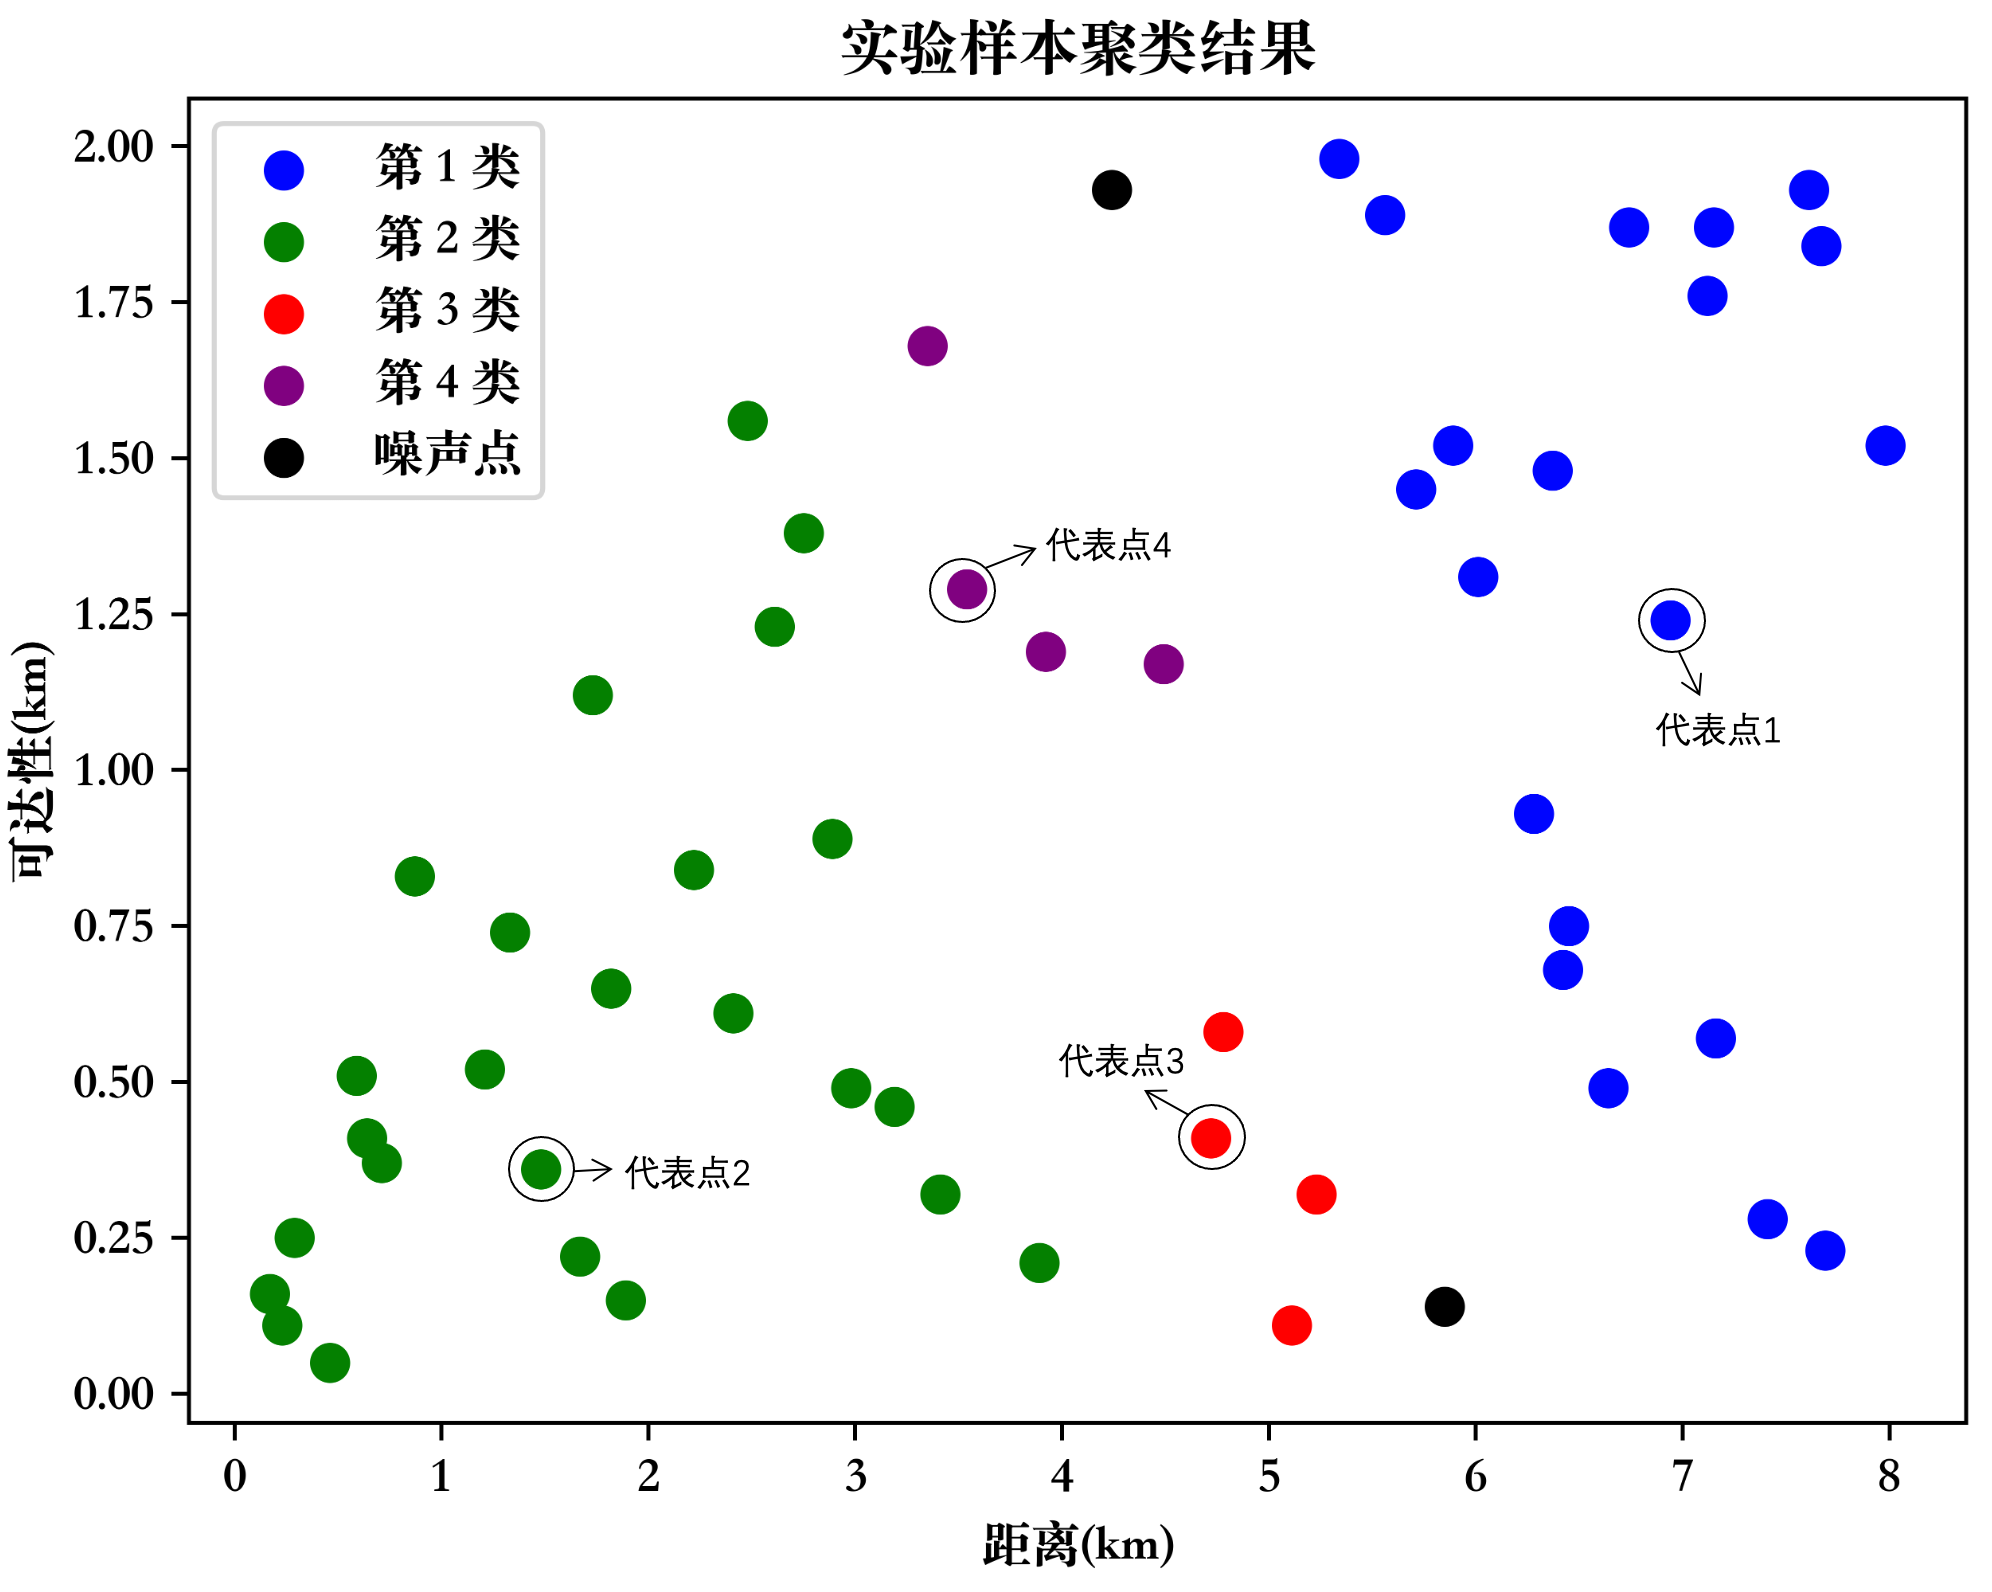
\includegraphics[width=.75\linewidth]{figures/content/db_cluster.png}
  \caption{代表智能体的位置示意图}
  \label{db_cluster}
\end{figure}


\subsection{训练及结果分析}

在本文中,采用深度Q网络算法来优化出行模式和出发时间的选择,以获得最佳的出行体验。有数值实验均在标准计算机上进行,配置为Intel Core (TM) i5-9400F 2.90 GHz CPU和8 GB RAM。将训练过程设置为800个episode。在每个时间步长内,智能体根据当前状态选择一个动作,然后接收到环境返回的奖励,并转移到下一个状态。我们使用$\varepsilon$-贪婪策略来探索动作空间,其中$\varepsilon$在前400个episode中线性下降到0.1,然后保持不变。在探索时,智能体将以$\varepsilon$的概率选择一个随机动作,否则将根据当前Q值估计选择一个最佳动作。

使用SUMO仿真工具来模拟城市交通网络,四个代表智能体的OD在网络中的位置如图\ref{agent_map}所示,将智能体的行为应用于仿真中的出行模式选择和出发时间选择中。根据仿真结果,可以获得出行时间、路线和交通方式等方面的信息,以评估该算法的性能。
\begin{figure}
  \centering
  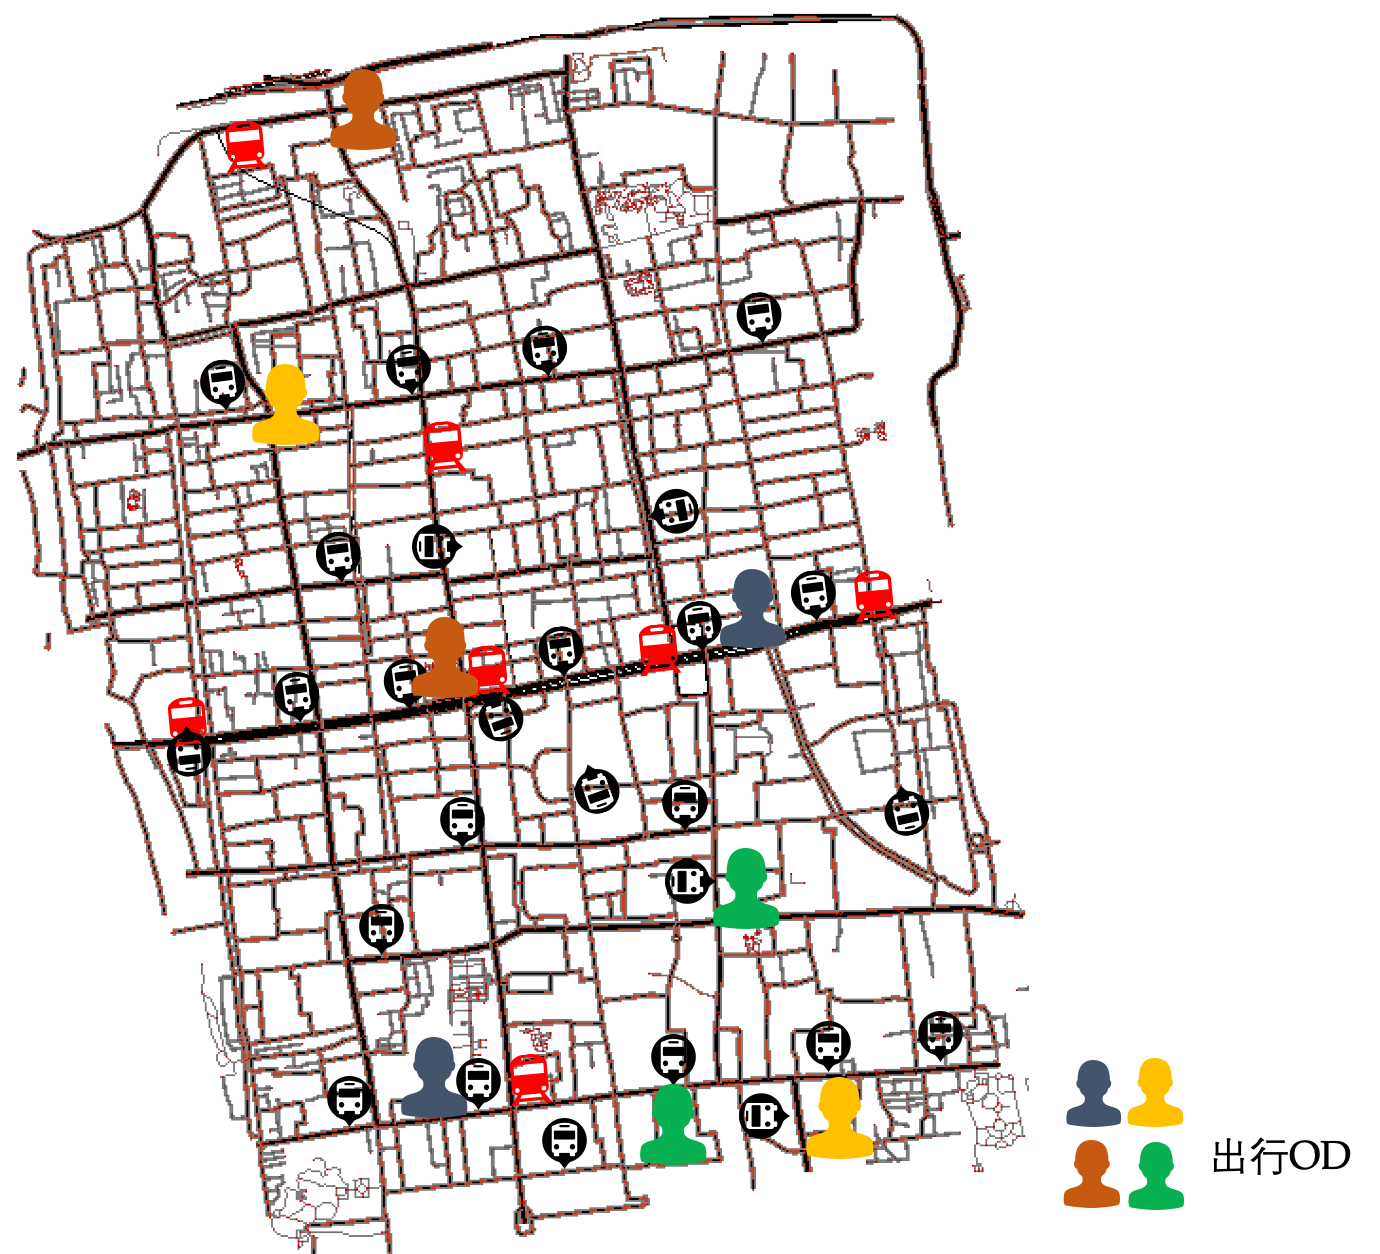
\includegraphics[width=.75\linewidth]{figures/content/agent_map.png}
  \caption{代表智能体的位置示意图}
  \label{agent_map}
\end{figure}

首先,在训练过程中设置了一个经验回放机制。该机制用于存储代理在仿真环境中所经历的状态、动作、奖励和下一状态等信息,并且按照一定的概率进行抽样,以保证数据的独立性和随机性。其次,采用目标网络的方法来减小估计误差的影响。在训练过程中使用了两个神经网络,即一个本地网络和一个目标网络。本地网络用于根据当前状态计算Q值,而目标网络则用于计算目标Q值。在一定的时间间隔内,目标网络的参数会从本地网络中更新,以缓解估计误差的影响。最后,将使用Adam优化器来对网络进行训练,以提高算法的收敛速度和性能。

图 \ref{loss&reward} 显示了在训练800个周期中损失值和奖励值的收敛模式变化。在损失值变化图像中,整体呈现出明显的下降趋势,这与期望相符。在训练初期,由于智能体在训练开始阶段需要对环境进行行动探索,因此损失函数值波动较大。然而,这种波动主要集中在前300个周期,并且持续时间相对较短。实际上,从大约第500个周期开始,损失函数值的变化微小,几乎呈直线趋势。这一观察结果明确地证实了算法的收敛性。从图中可以看出,本文提出的深度强化学习算法在训练过程中表现良好,并已在此任务上达到收敛。为了评估算法在此任务上的性能,可以计算平均奖励值。在训练过程中,每个代表个体通过遵循深度强化学习推荐的行动所获得的奖励的变化结果如图 \ref{loss&reward}(b)所示。考虑到每个代表个体的旅行都具有不同的OD,相关的奖励大小也不同。事实上,可以轻易地发现,智能体1可能会有最长的旅行,而智能体3和4可能会有较短的旅行。然而,无论奖励的绝对值如何,所有代表个体的曲线都呈现出增长的趋势,这意味着他们通过与环境的交互并学习不断改进他们的旅行选择。在大约700个阶段内,每个代表的奖励基本稳定,并且此后变化不大,这一观察结果与图 \ref{loss&reward}(a)一致。图 \ref{loss&reward} 的结果表明,通过使用深度强化学习,智能体能够有效地学习并逐渐改善其决策。在训练过程中,智能体能够对环境进行探索,并通过与环境的交互学习如何选择最优的行动,从而最小化旅行时间和出行成本。此外,随着训练周期的增加,智能体的学习能力逐渐提高,同时收敛速度也变得更快。
\begin{figure}
\centering
  \subfloat[损失值变化图像]{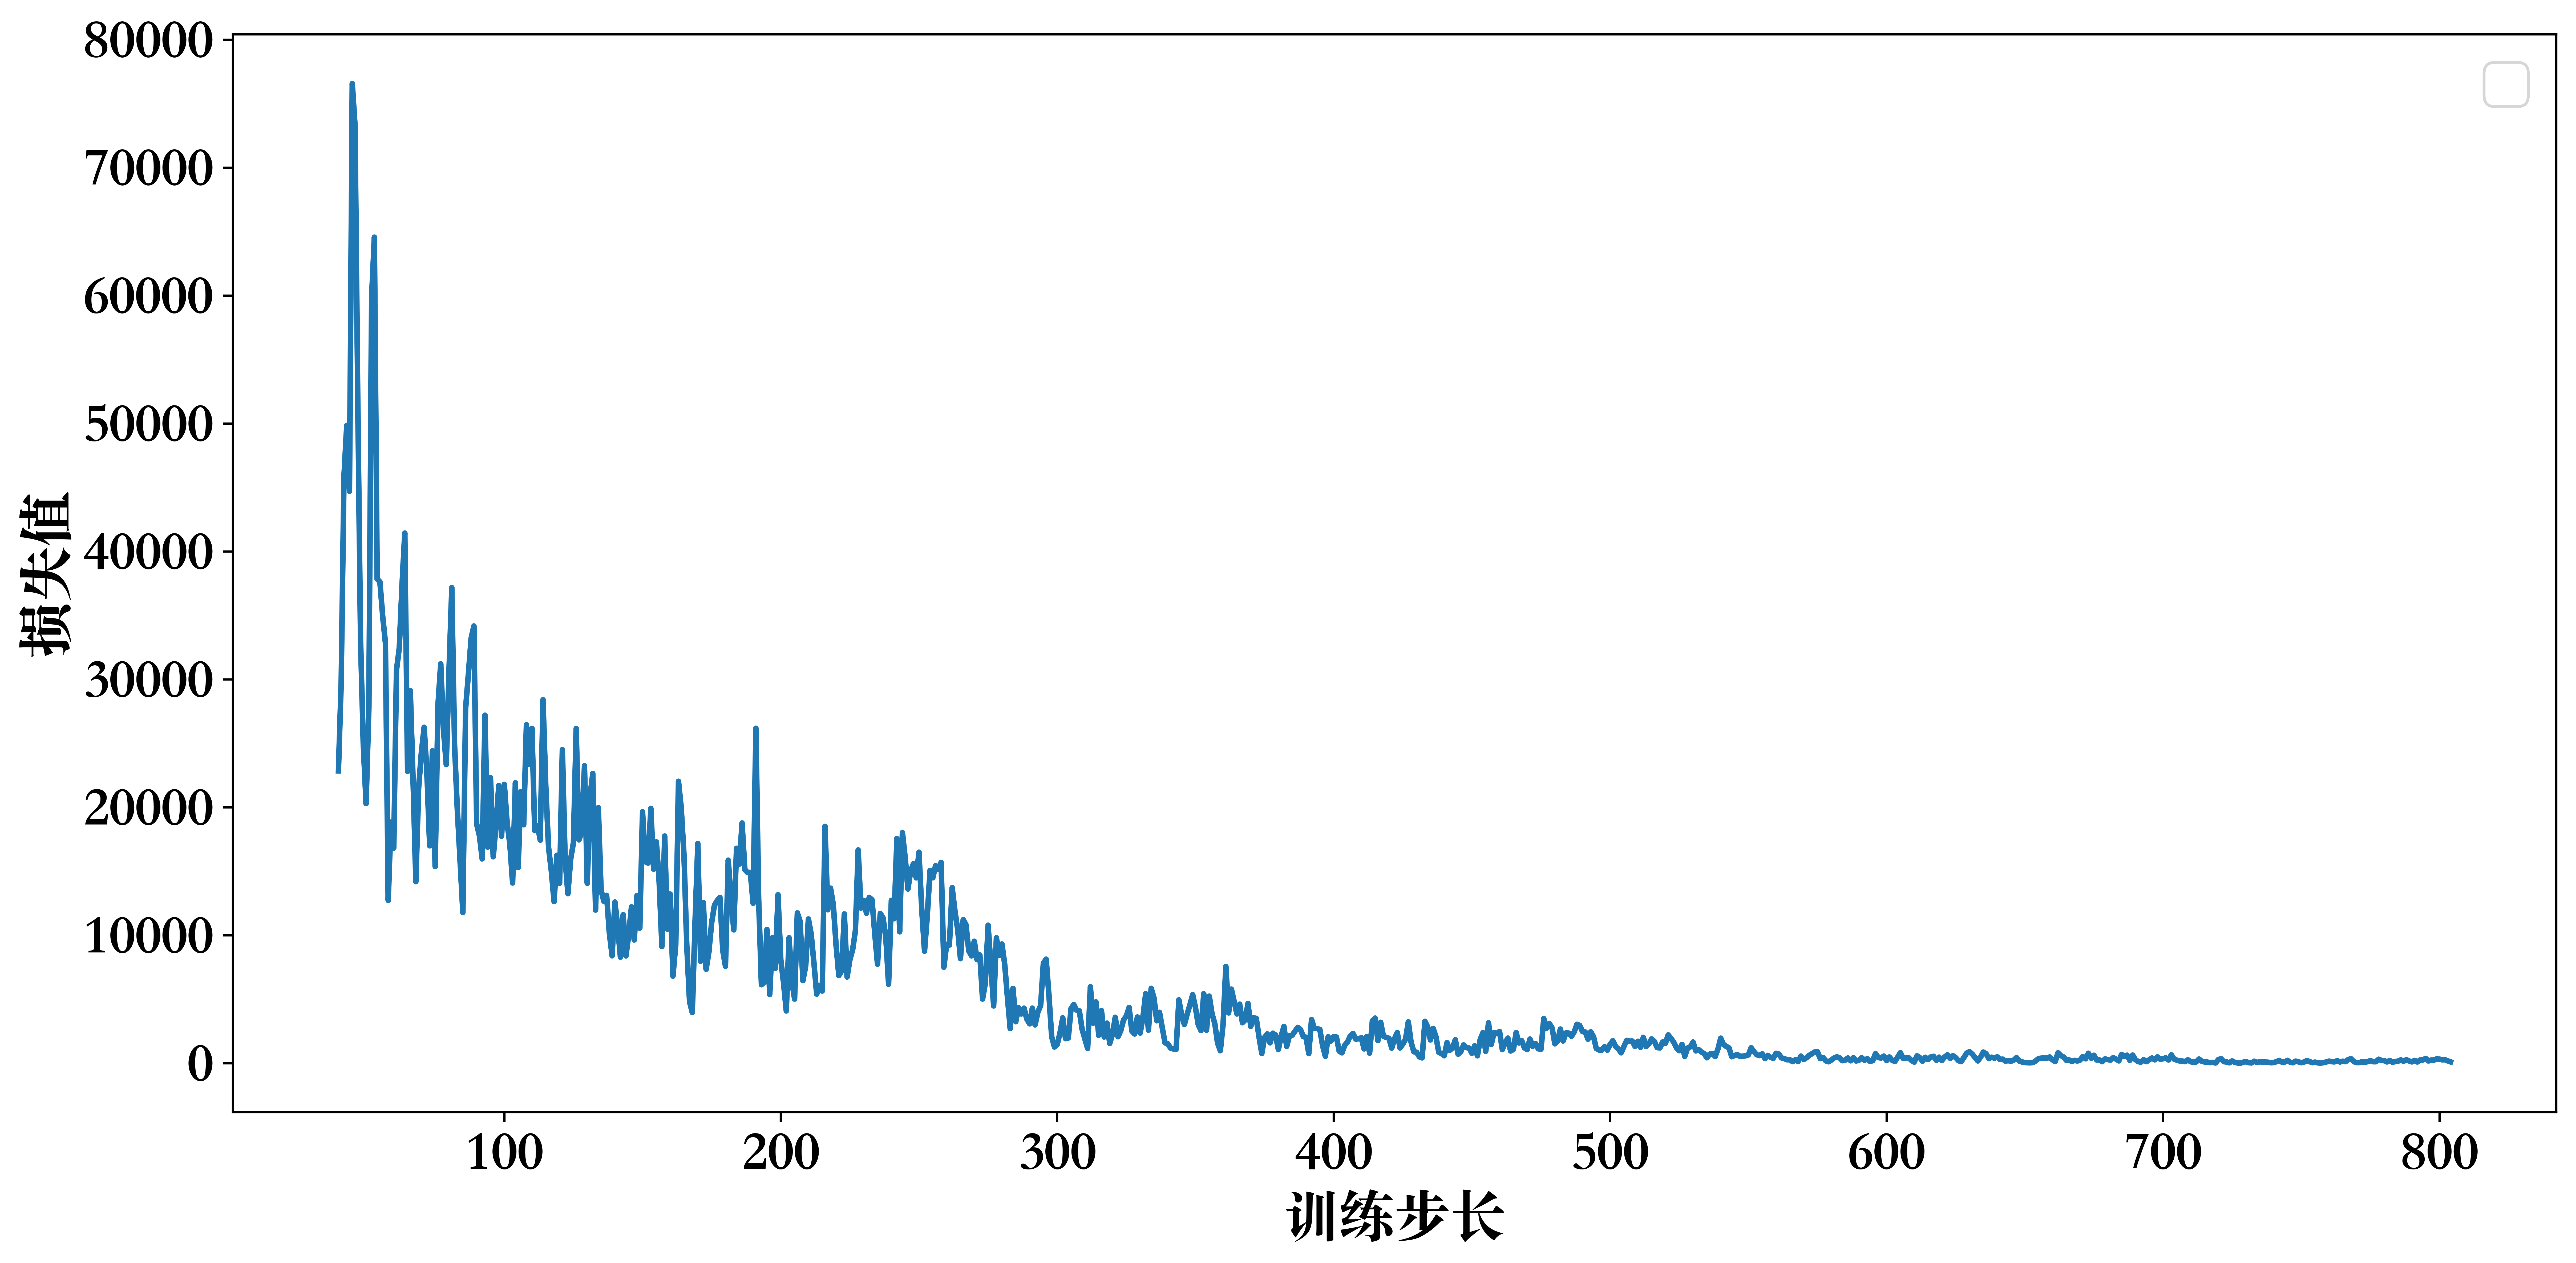
\includegraphics[width=.85\textwidth]{figures/content/loss.png}}
  \label{loss}
  \\
  \subfloat[奖励变化图像]{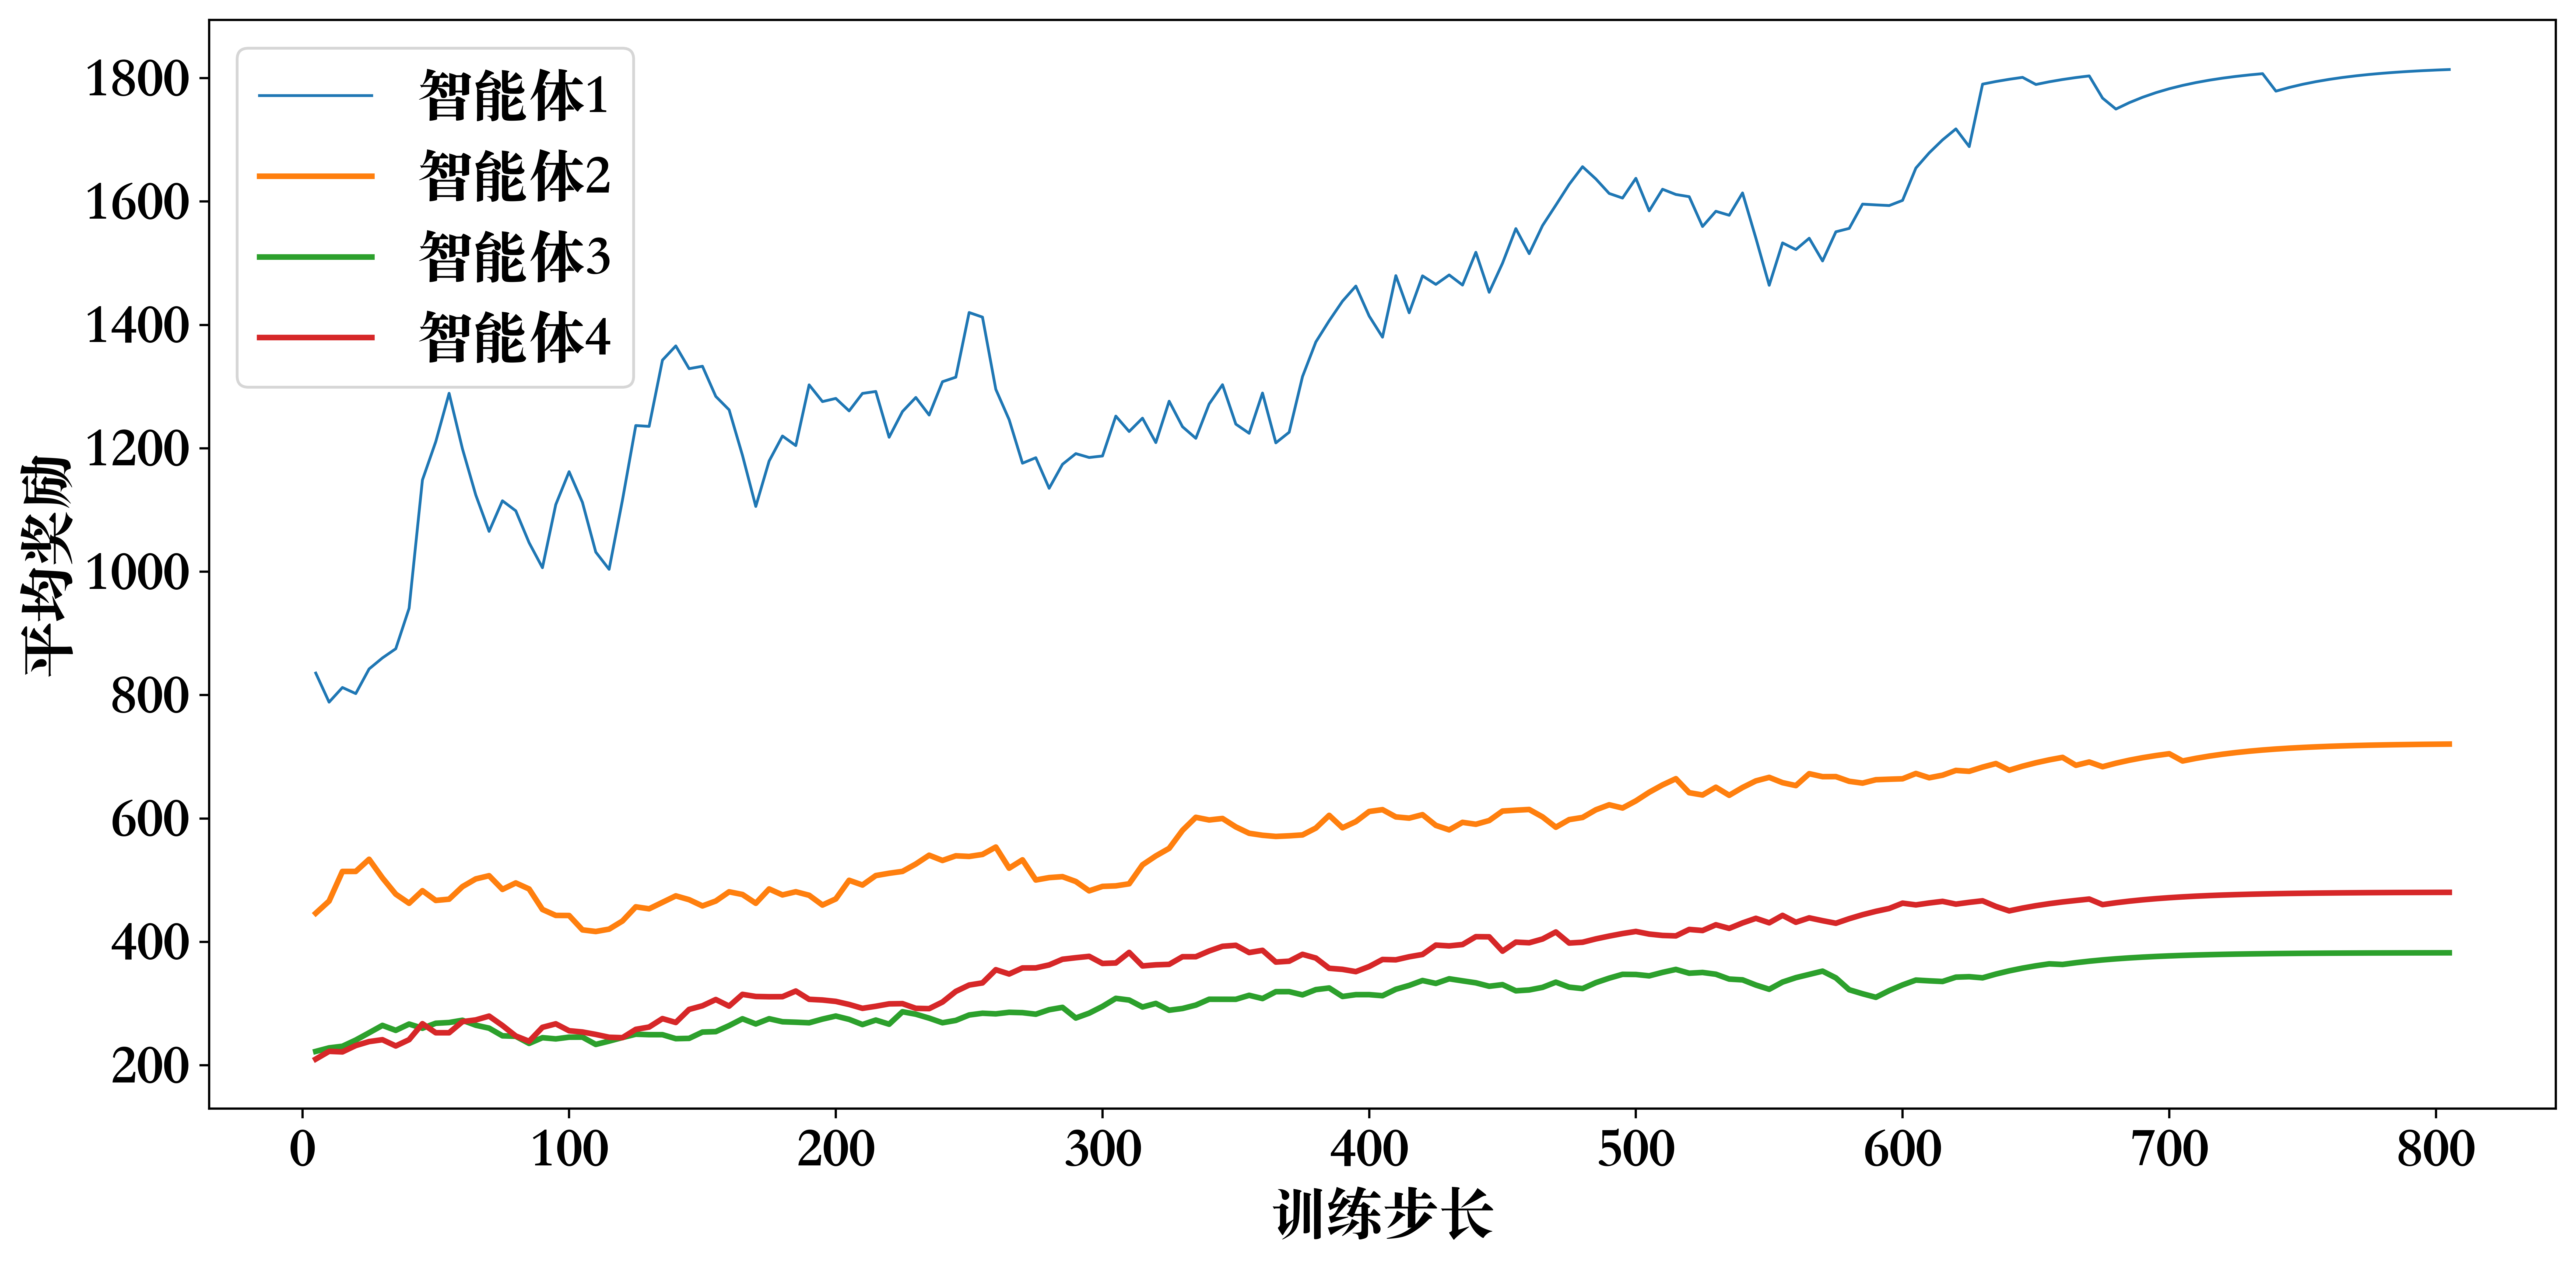
\includegraphics[width=.85\textwidth]{figures/content/reward.png}}
  \label{reward}
  \caption{训练过程中各个代表智能体损失值与奖励值的变化图像}
  \label{loss&reward}
\end{figure}

图\ref{agents}中展示了四个代表性个体在训练过程中遵循的深度强化学习建议行动。初始阶段,智能体的行动变化频繁,这是由于行动探索阶段所导致的。在这个阶段,智能体个体主要通过不断地尝试来了解环境并寻找最佳策略。由于环境的不确定性,智能体可能会尝试多种不同的行动,以了解每种行动的结果和潜在收益。但是,一旦智能体个体进入利用阶段,它们开始依赖其已经学习到的知识和经验,从而选择能够带来最大收益的行动。在这个阶段,由于智能体个体已经建立了一个比较准确的环境模型和策略,所以行动变化的波动性逐渐减小,每个智能体个体似乎已经找到了其自身出行模式与出发时间的最优解。在利用阶段期间,智能体个体偶尔会进行一些行动更改,这可能是由于$\varepsilon$-贪心策略所导致的。$\varepsilon$-贪心策略是一种在训练初期使用的策略,其目的是在探索阶段时增加行动的随机性,从而帮助智能体个体更好地了解环境。随着训练的进行,$\varepsilon$的值逐渐降低到一个非常小的值,从而逐渐减小了随机性,使得智能体个体的行动更加稳定和准确。总的来说,这些观察结果表明,深度强化学习算法在训练过程中,智能体个体通过探索与利用阶段的交替学习,最终学会了最优策略,并且能够在不同的情况下做出正确的决策。


\begin{figure}[htbp]
  \subfloat[智能体1]{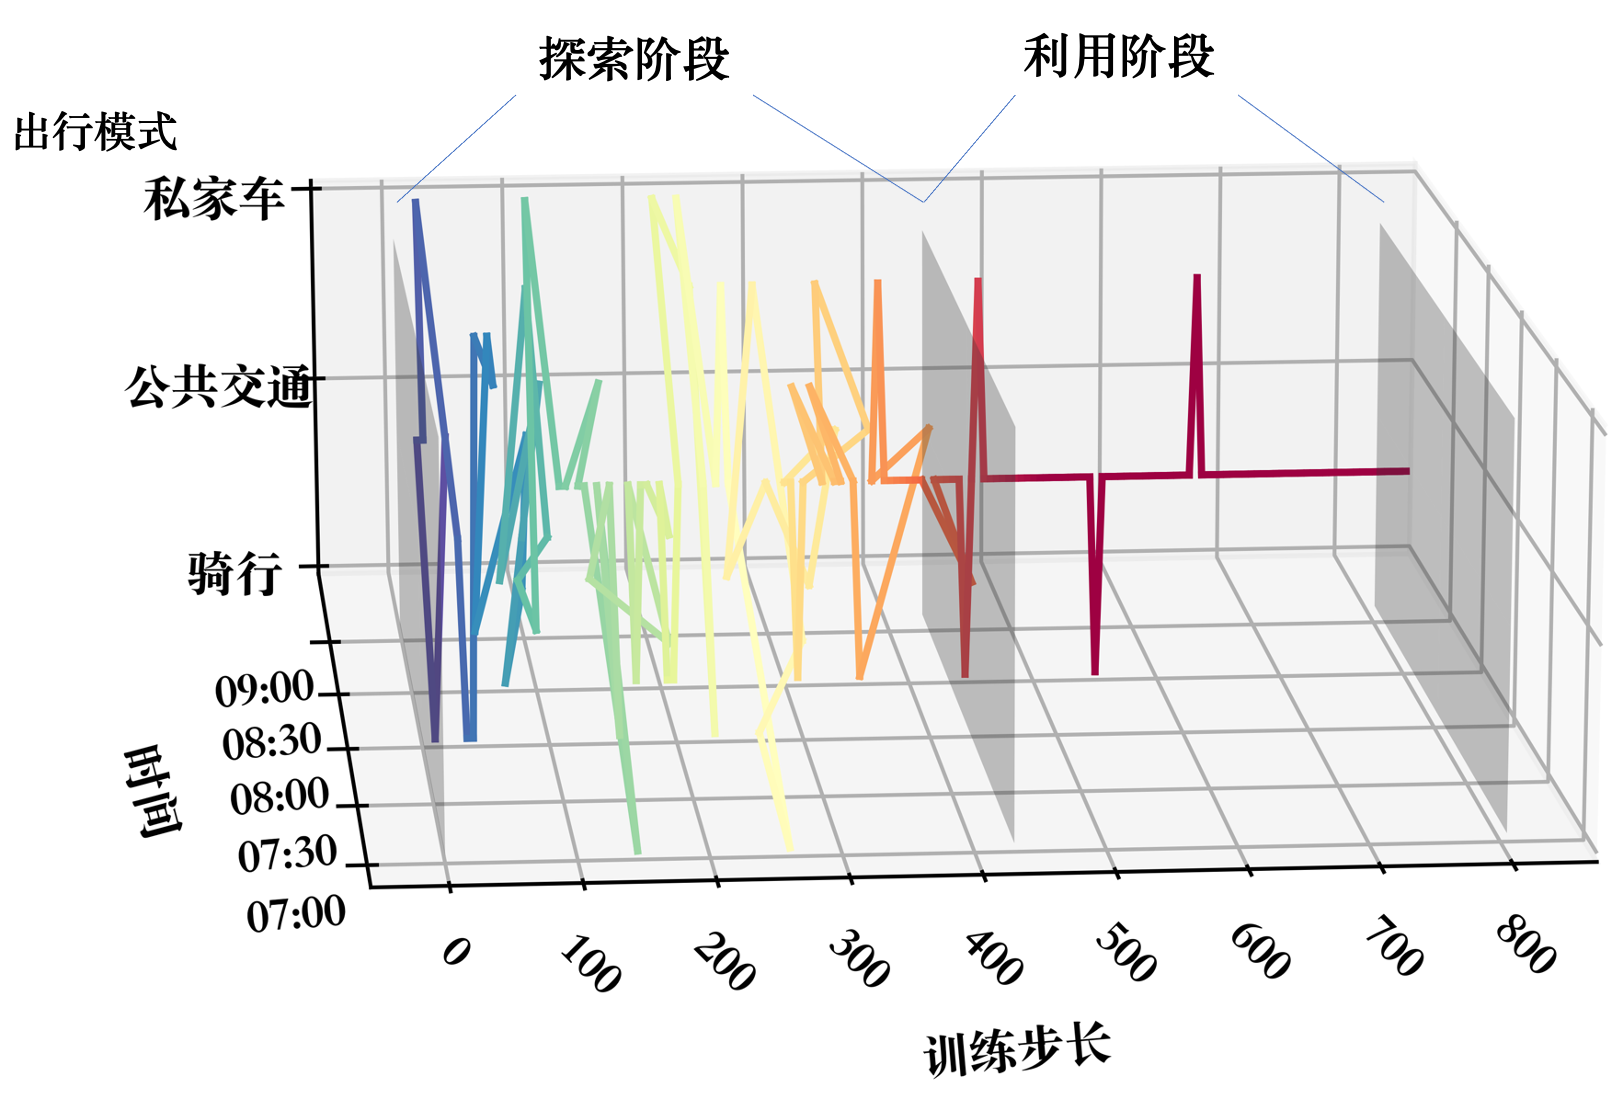
\includegraphics[width=.5\textwidth]{figures/content/action1.png}}
  \quad\quad
  \subfloat[智能体2]{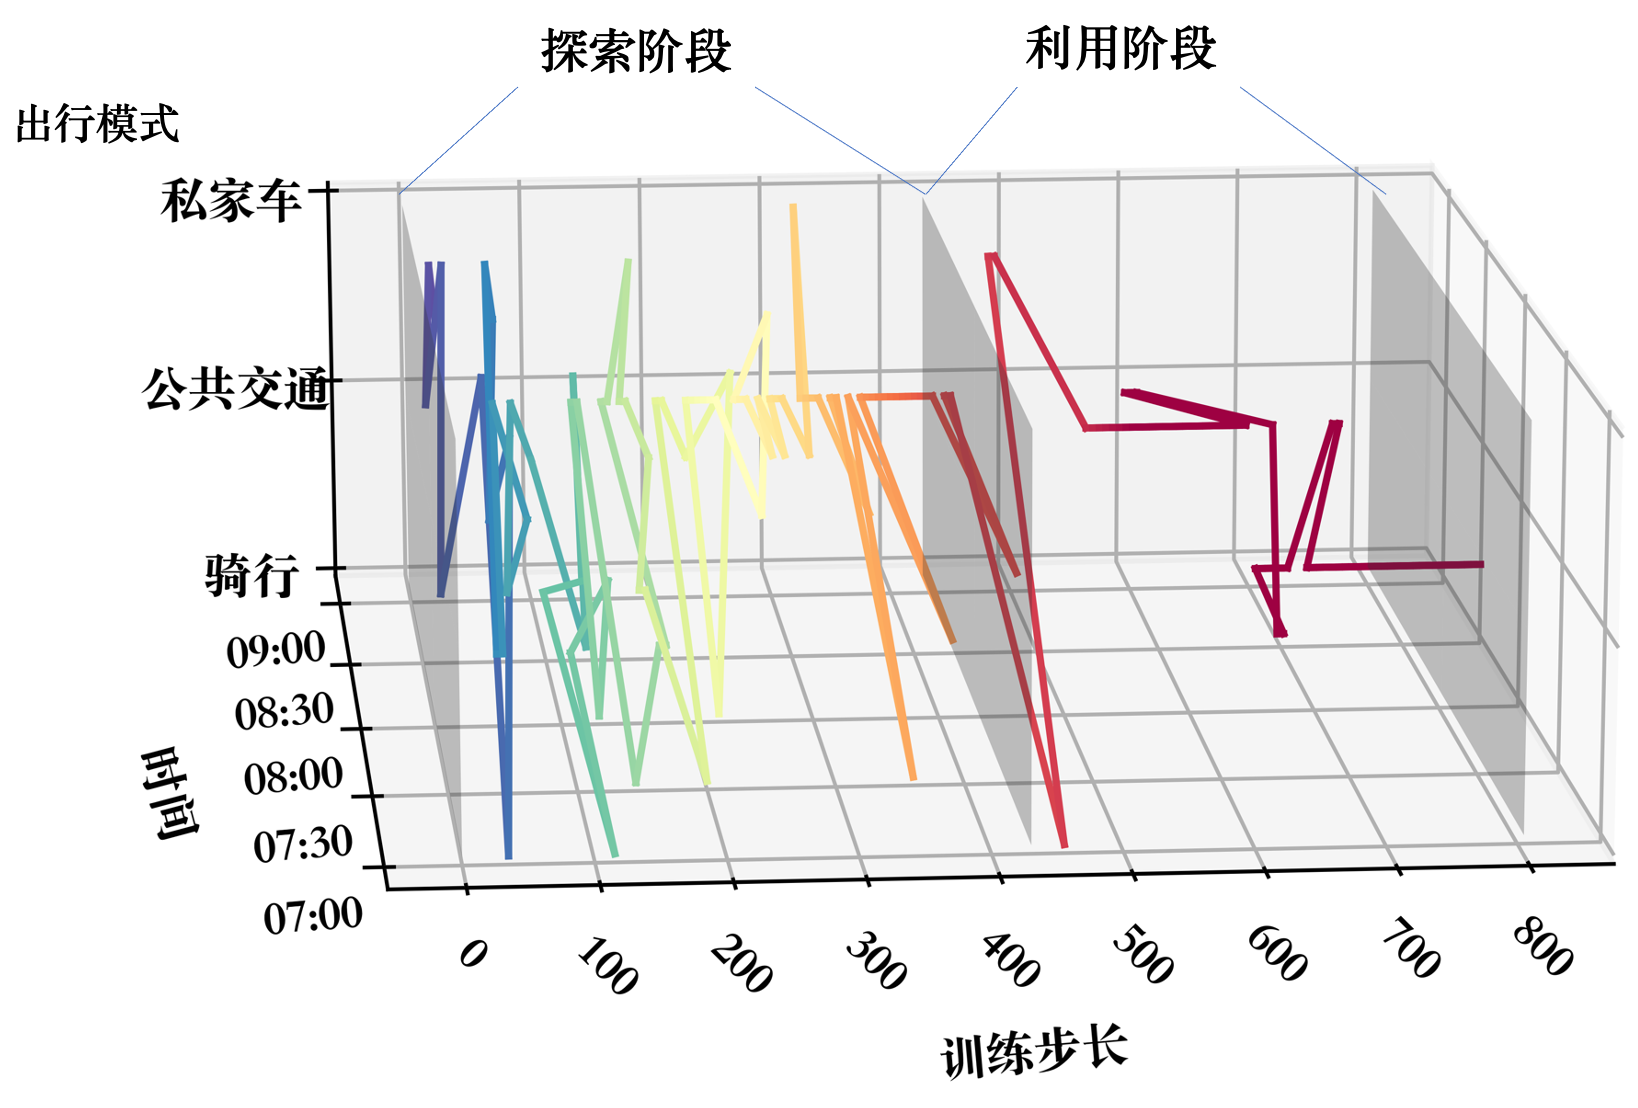
\includegraphics[width=.5\textwidth]{figures/content/action2.png}}
  \\
  \subfloat[智能体3]{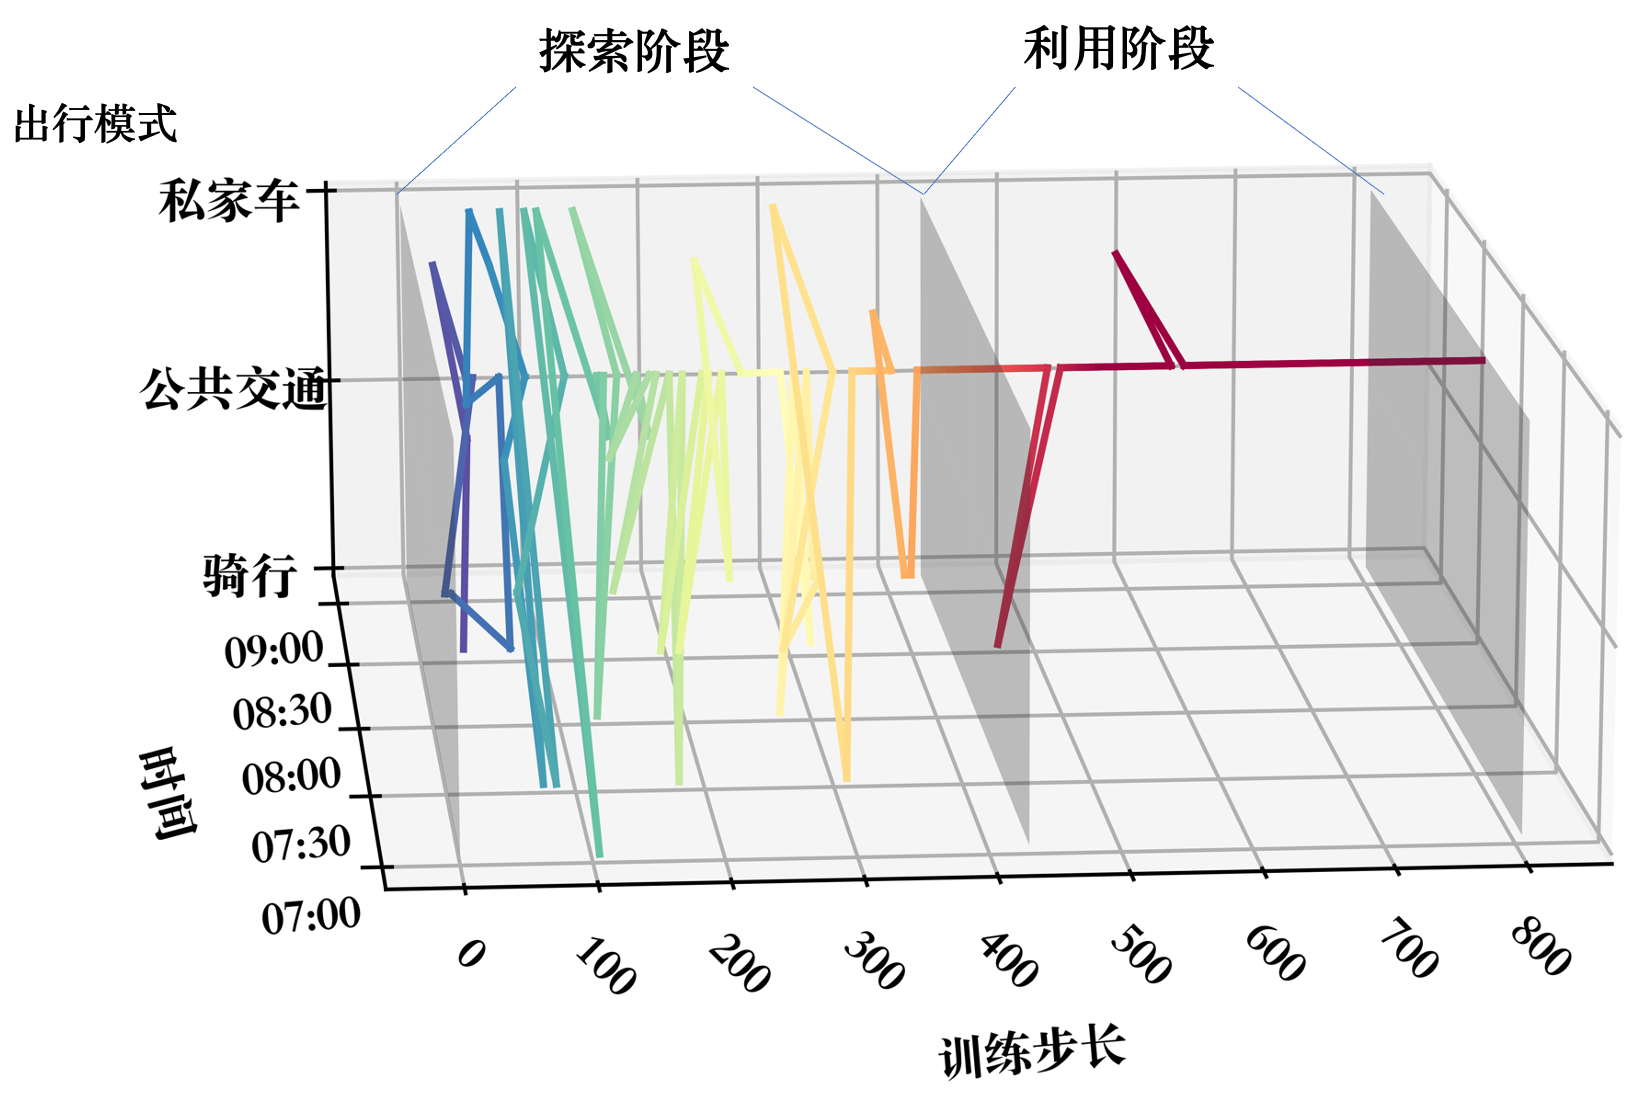
\includegraphics[width=.5\textwidth]{figures/content/action3.png}}
  \quad\quad
  \subfloat[智能体4]{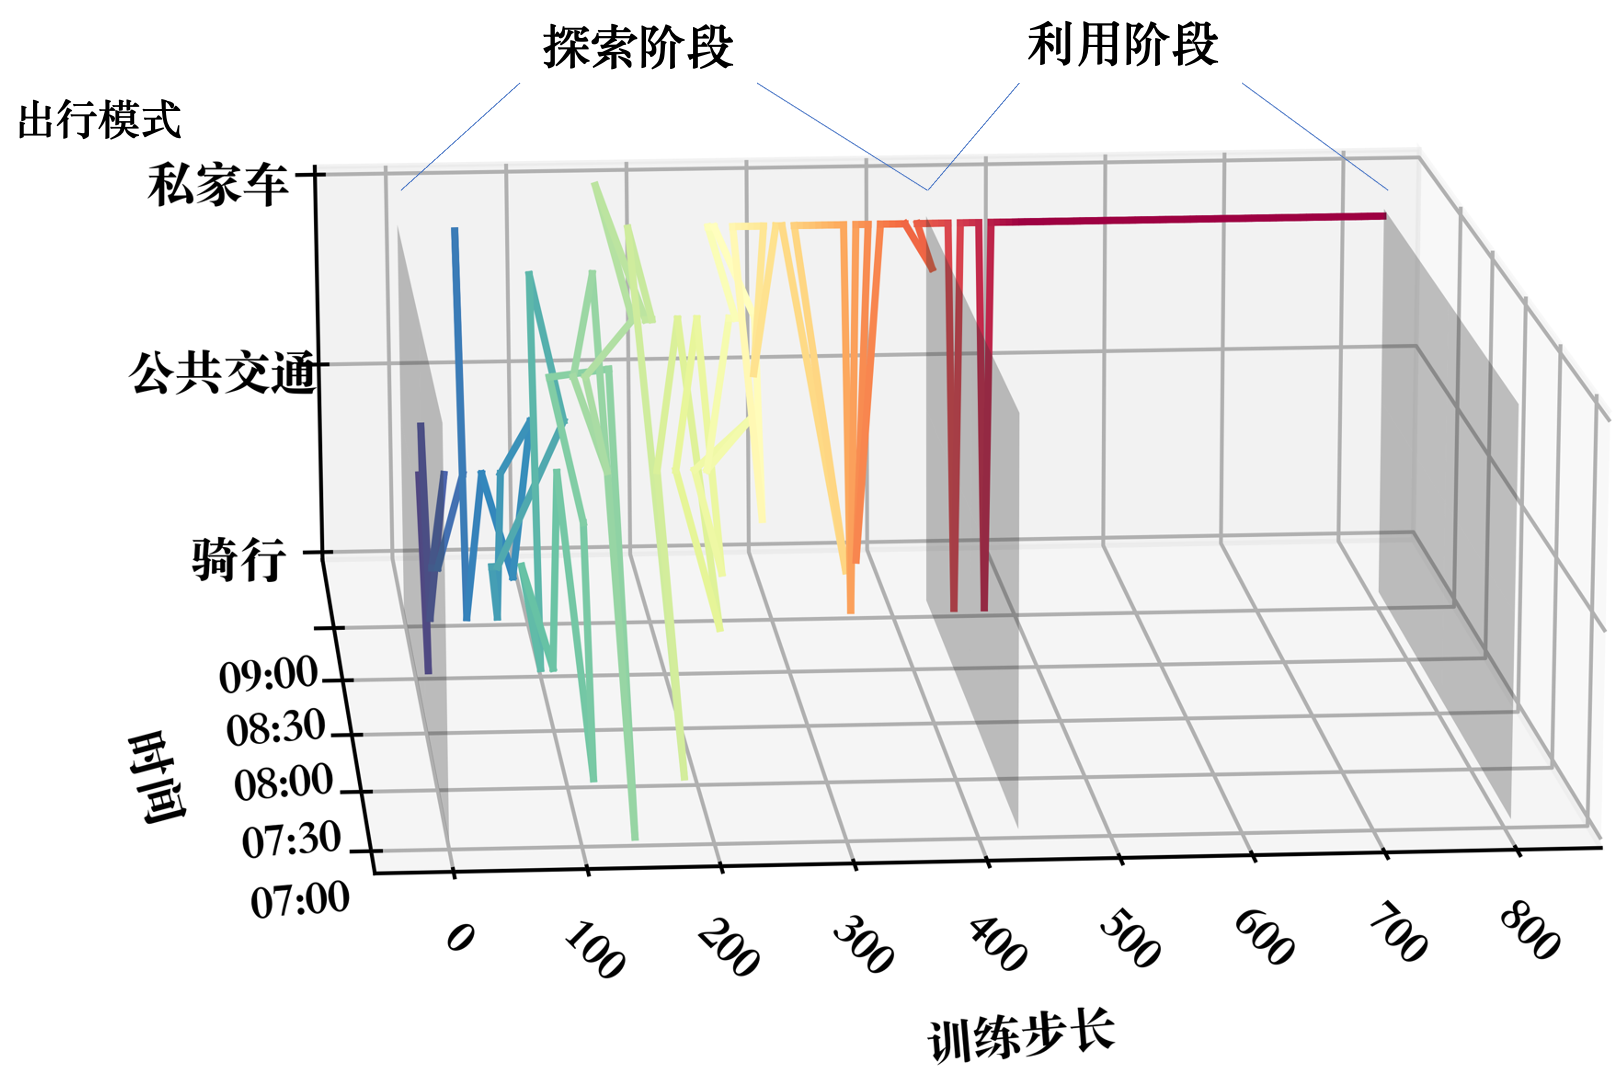
\includegraphics[width=.5\textwidth]{figures/content/action4.png}}
  \caption{训练过程中代表智能体的动作选择变化}
  \label{agents}
\end{figure}




\section{模型的评估}
\label{section:5.2}

在本节中,将对基于深度强化学习的出行模式与时间选择模型进行评估,其目的在于验证模型的有效性和泛化能力。本节将分别从模型泛化能力检验、与传统方法的对比和模型参数的灵敏度分析三个方面对模型进行评估。在泛化能力检验中,使用测试集对模型进行测试,以验证其在不同数据集上的表现;在对比传统方法方面,将使用传统的离散选择方法与深度强化学习方法进行对比,并分析两者的优劣势;最后,在参数灵敏度分析中,将探讨模型参数对模型表现的影响,以确定模型最优参数。

\subsection{模型泛化能力检验}

为了对模型的泛化能力进行了测试,从训练数据中随机选取一部分个体,并将其作为测试集。然后对这些测试集中的个体进行测试,并计算其平均奖励值。为了检验所提出方法得到的解决方案的优劣或最优性,将所提出的方法与传统DQN方法和朴素法进行比较。传统DQN方法是一种已经被广泛研究和应用的深度强化学习方法,因此可以作为一个有代表性的基准。而朴素法是一种简单的贪心算法,它的性能不如传统DQN和所提出的方法,但它的计算复杂度很低,因此可以作为一种基准来比较所提出方法的性能。通过与传统DQN和朴素法的比较,可以验证本文方法的优越性和泛化能力。传统DQN方法与本文方法不同的是将只选择一个智能体样本进行训练。朴素法是在每个仿真中随机选择一个动作,为了充分探索动作空间,朴素法将运行1000个仿真次数。在这次比较分析中,测试数据集选择了网络中50个不同OD的出行个体,这些个体在训练中均没有被考虑。为了进行比较,让每个测试个体根据这些相互比较的决策者之一分别采取行动,并收集所得到的奖励。

图\ref{com}(a)、\ref{com}(b)和\ref{com}(c)展示了三个选定的测试个体的比较结果。结果表明,朴素法的奖励存在显著波动,因为随机选择的行动不能保证总是获得良好的结果。相比之下,所提出方法和普通DQN获得的奖励是与JTMDTC问题的最优解相关的单一值,如图中的直线所示。在这三个测试个体中,所提出方法给出的解决方案优于普通DQN,更优于大部分朴素法给出的解决方案,这一结果明显可见于图\ref{com}(a)和\ref{com}(c)。

为了更全面地了解所有50个测试个体的比较情况,找到了朴素法为每个测试个体获得的最大奖励,将其视为该个体出行模式和出发时间问题的近似最优解。将所提出方法和传统DQN给出的解决方案与这个参考值进行比较,可以从全局角度观察性能差异。图\ref{com}(d)显示,本文方法的大部分解决方案(超过40个)超过了参考奖励值的95\%,这意味着这些解决方案接近最优。然而,对于普通的DQN来说,情况并非如此。只有大约30\%的解决方案超过了同一参考值的95\%,还有相当多的解决方案甚至低于参考值的60\%。这些比较结果表明,所提出的方法在解决许多个体的出行模式和出发时间问题时具有有效性,并且代表在完成这个任务中所发挥的重要作用。由于测试个体并不是训练的一部分,结果表明所提出方法具有良好的可迁移性。

\begin{figure}[htbp]
  \subfloat[]{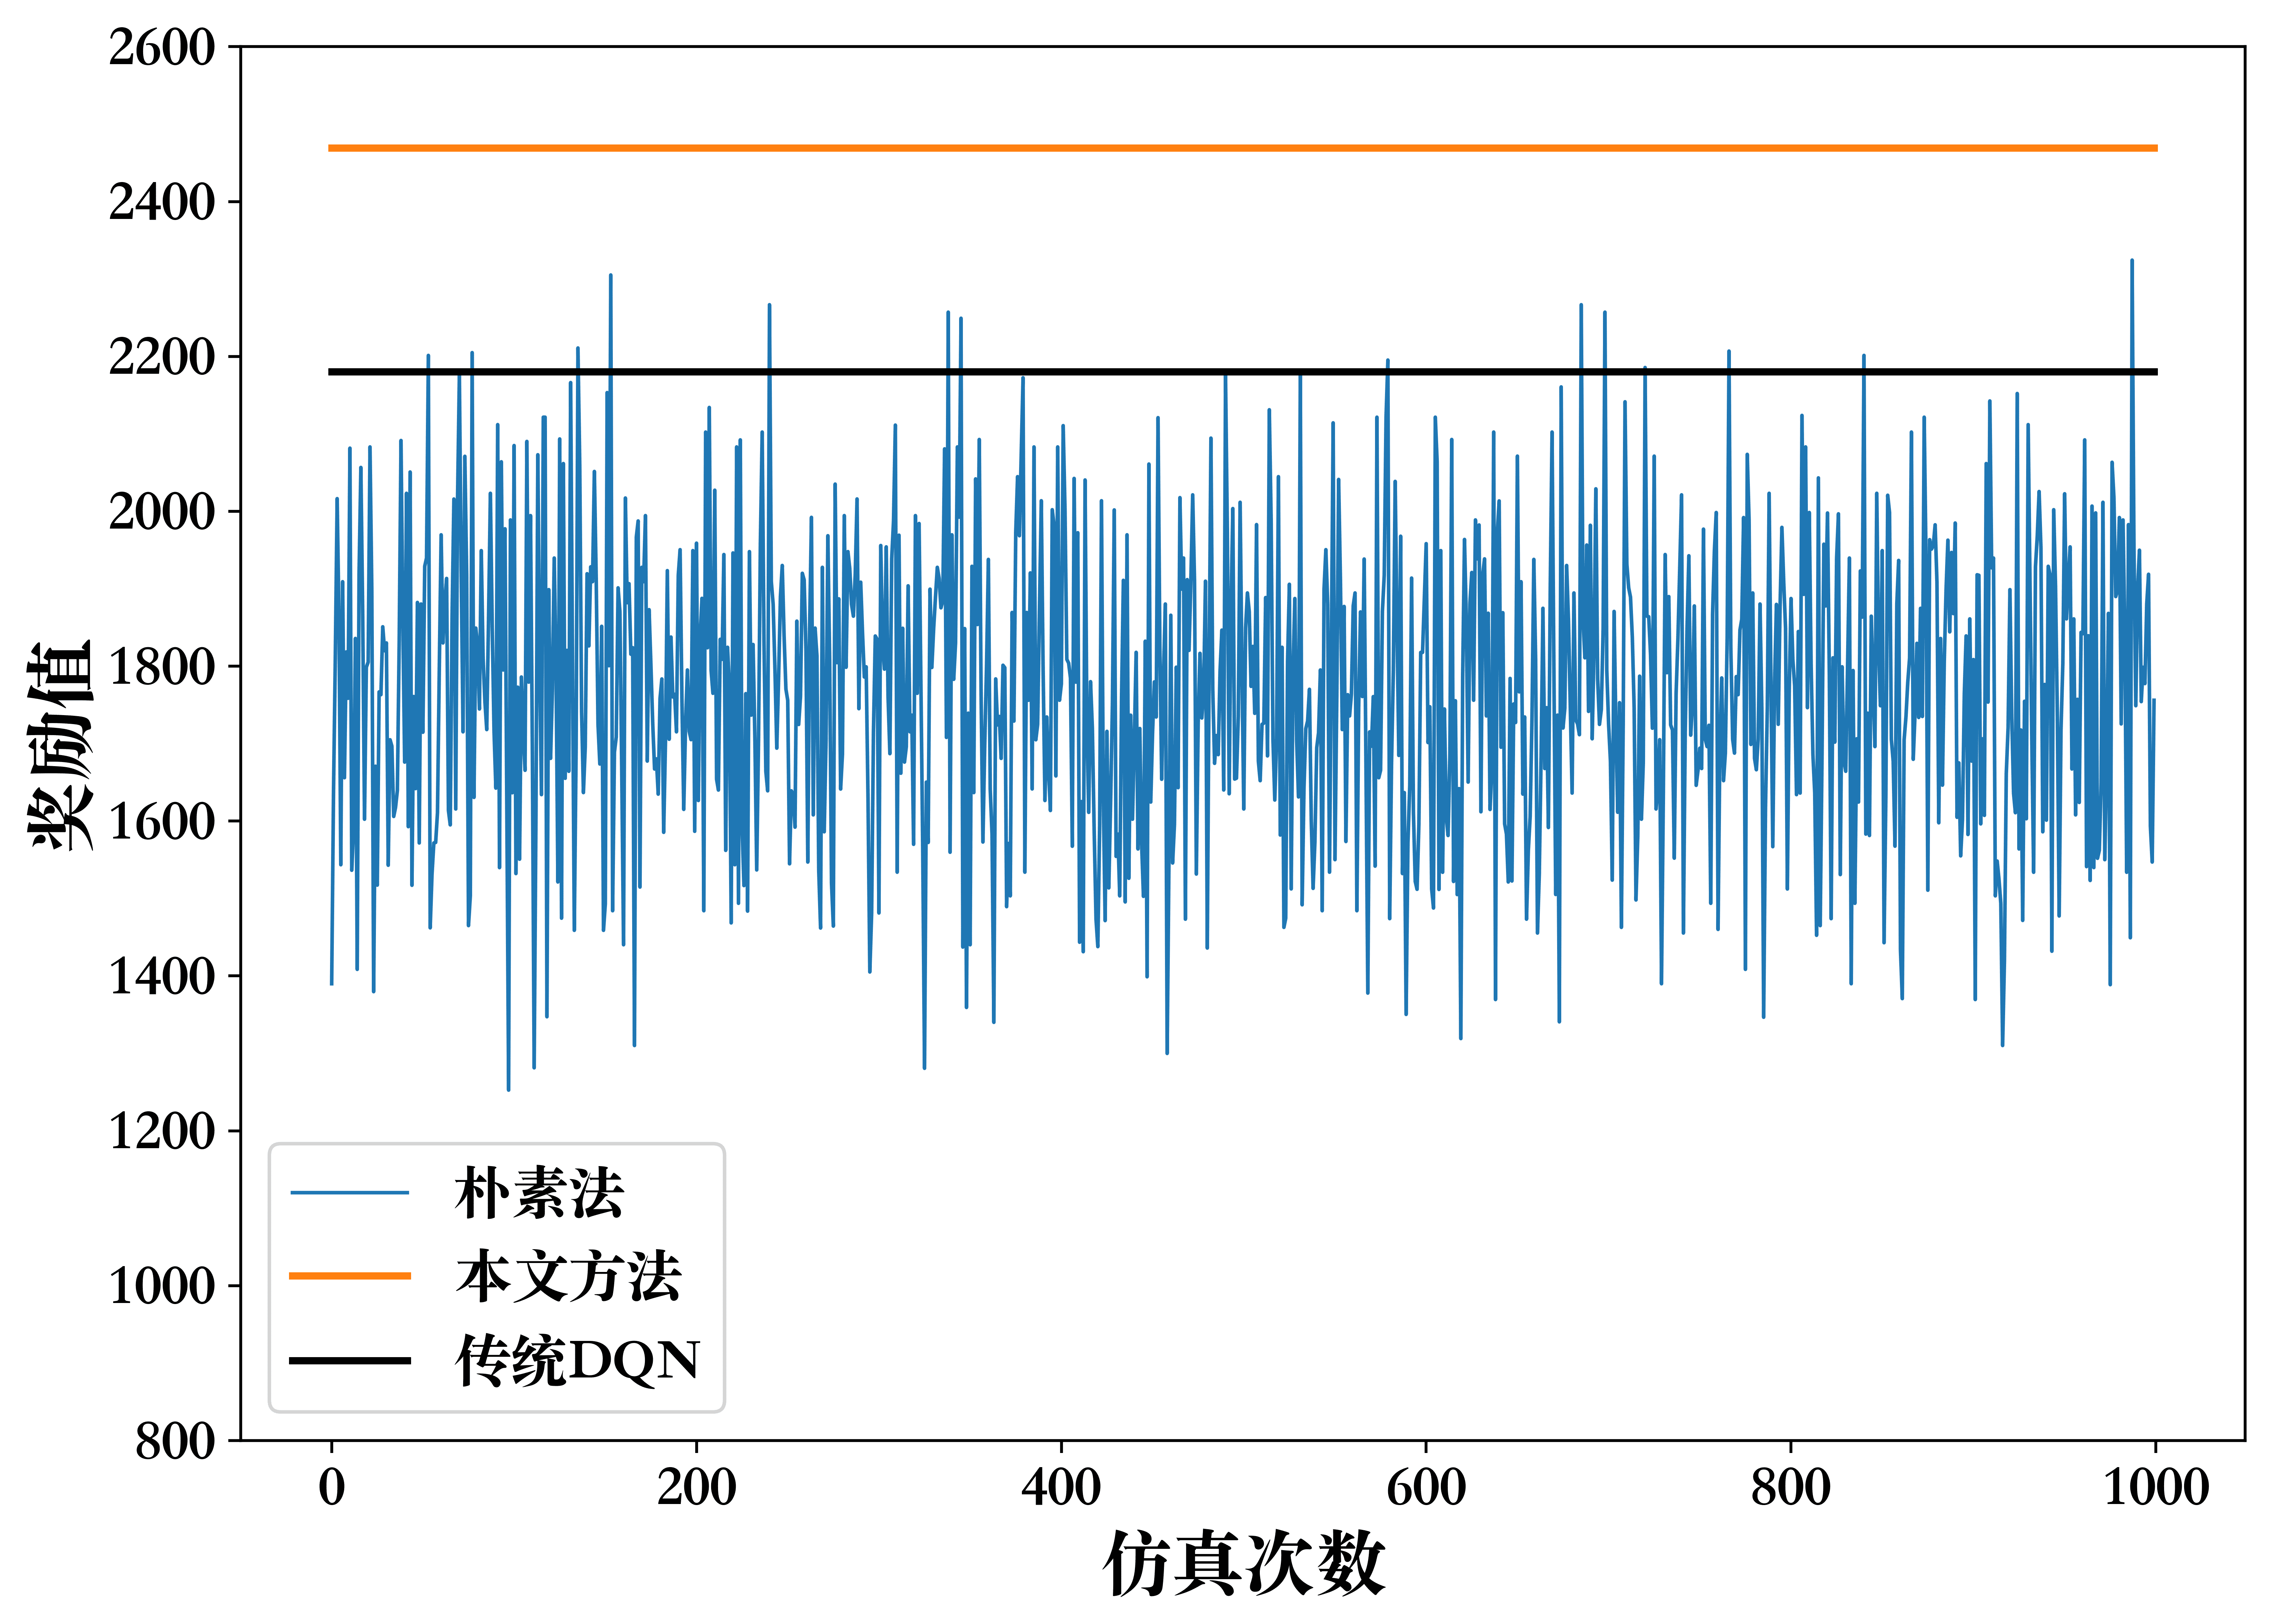
\includegraphics[width=.5\textwidth]{figures/content/com1.png}}
  \quad\quad
  \subfloat[]{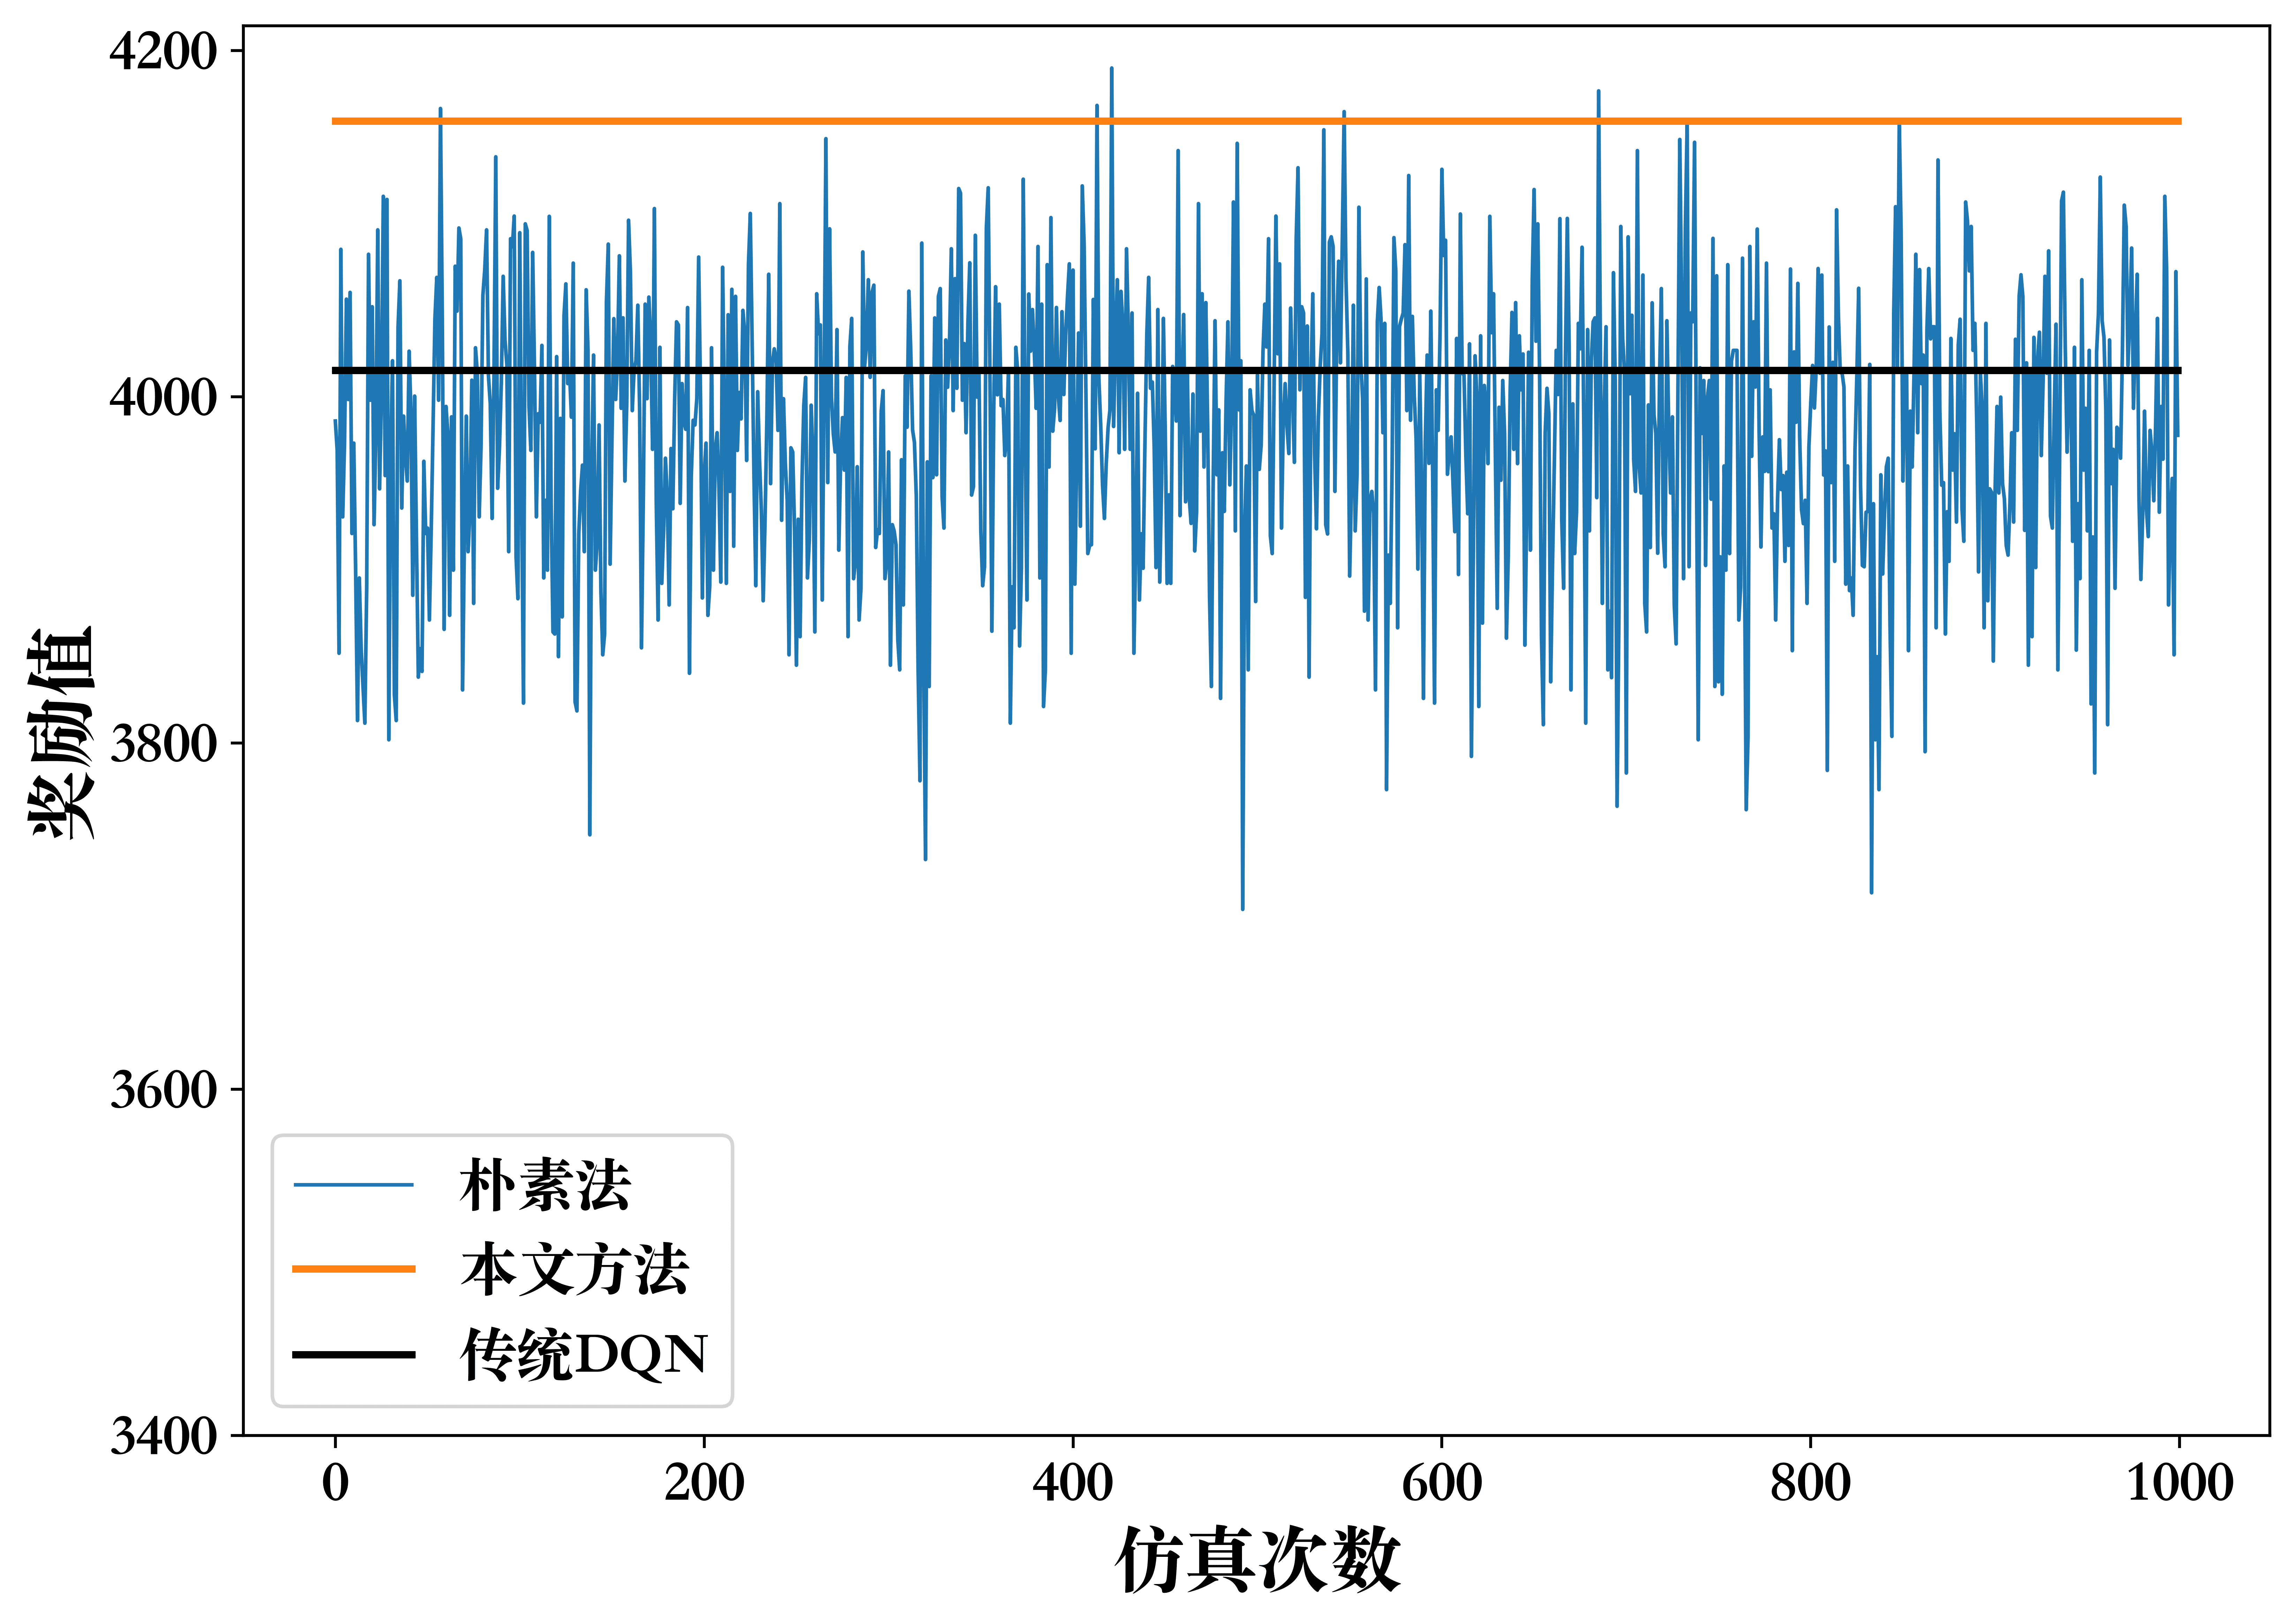
\includegraphics[width=.5\textwidth]{figures/content/com2.png}}
  \\
  \subfloat[]{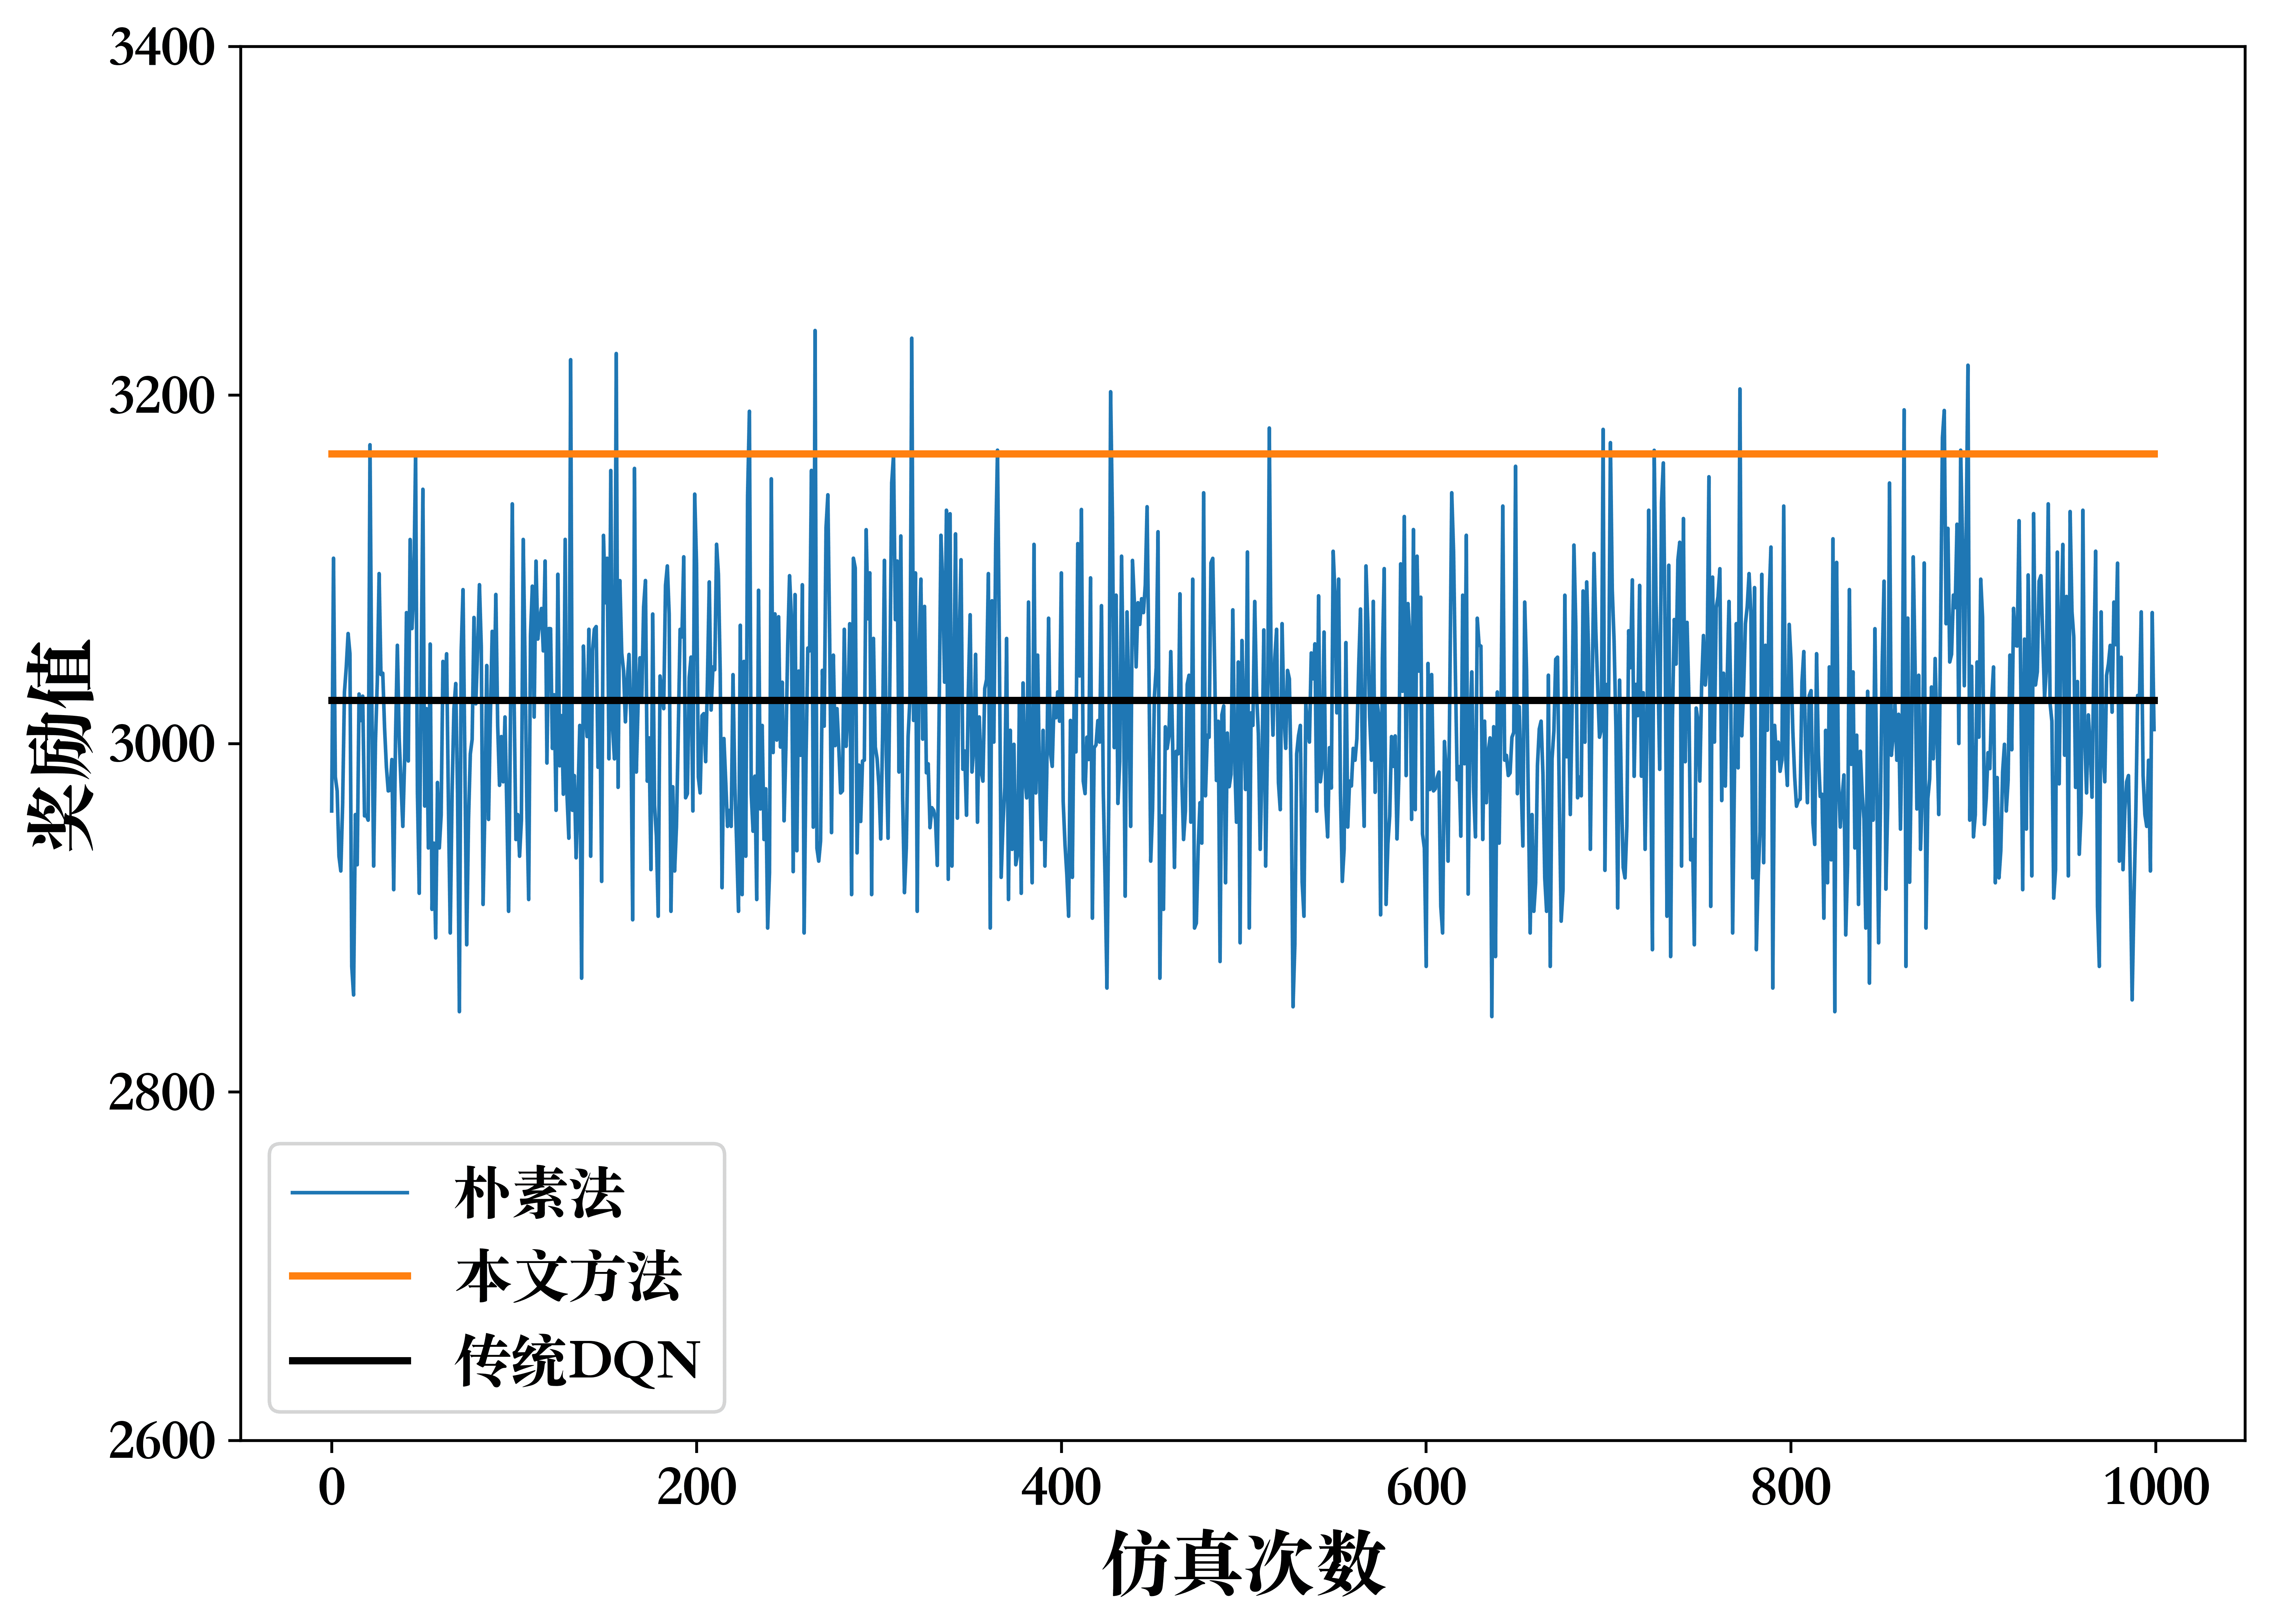
\includegraphics[width=.5\textwidth]{figures/content/com3.png}}
  \quad\quad
  \subfloat[]{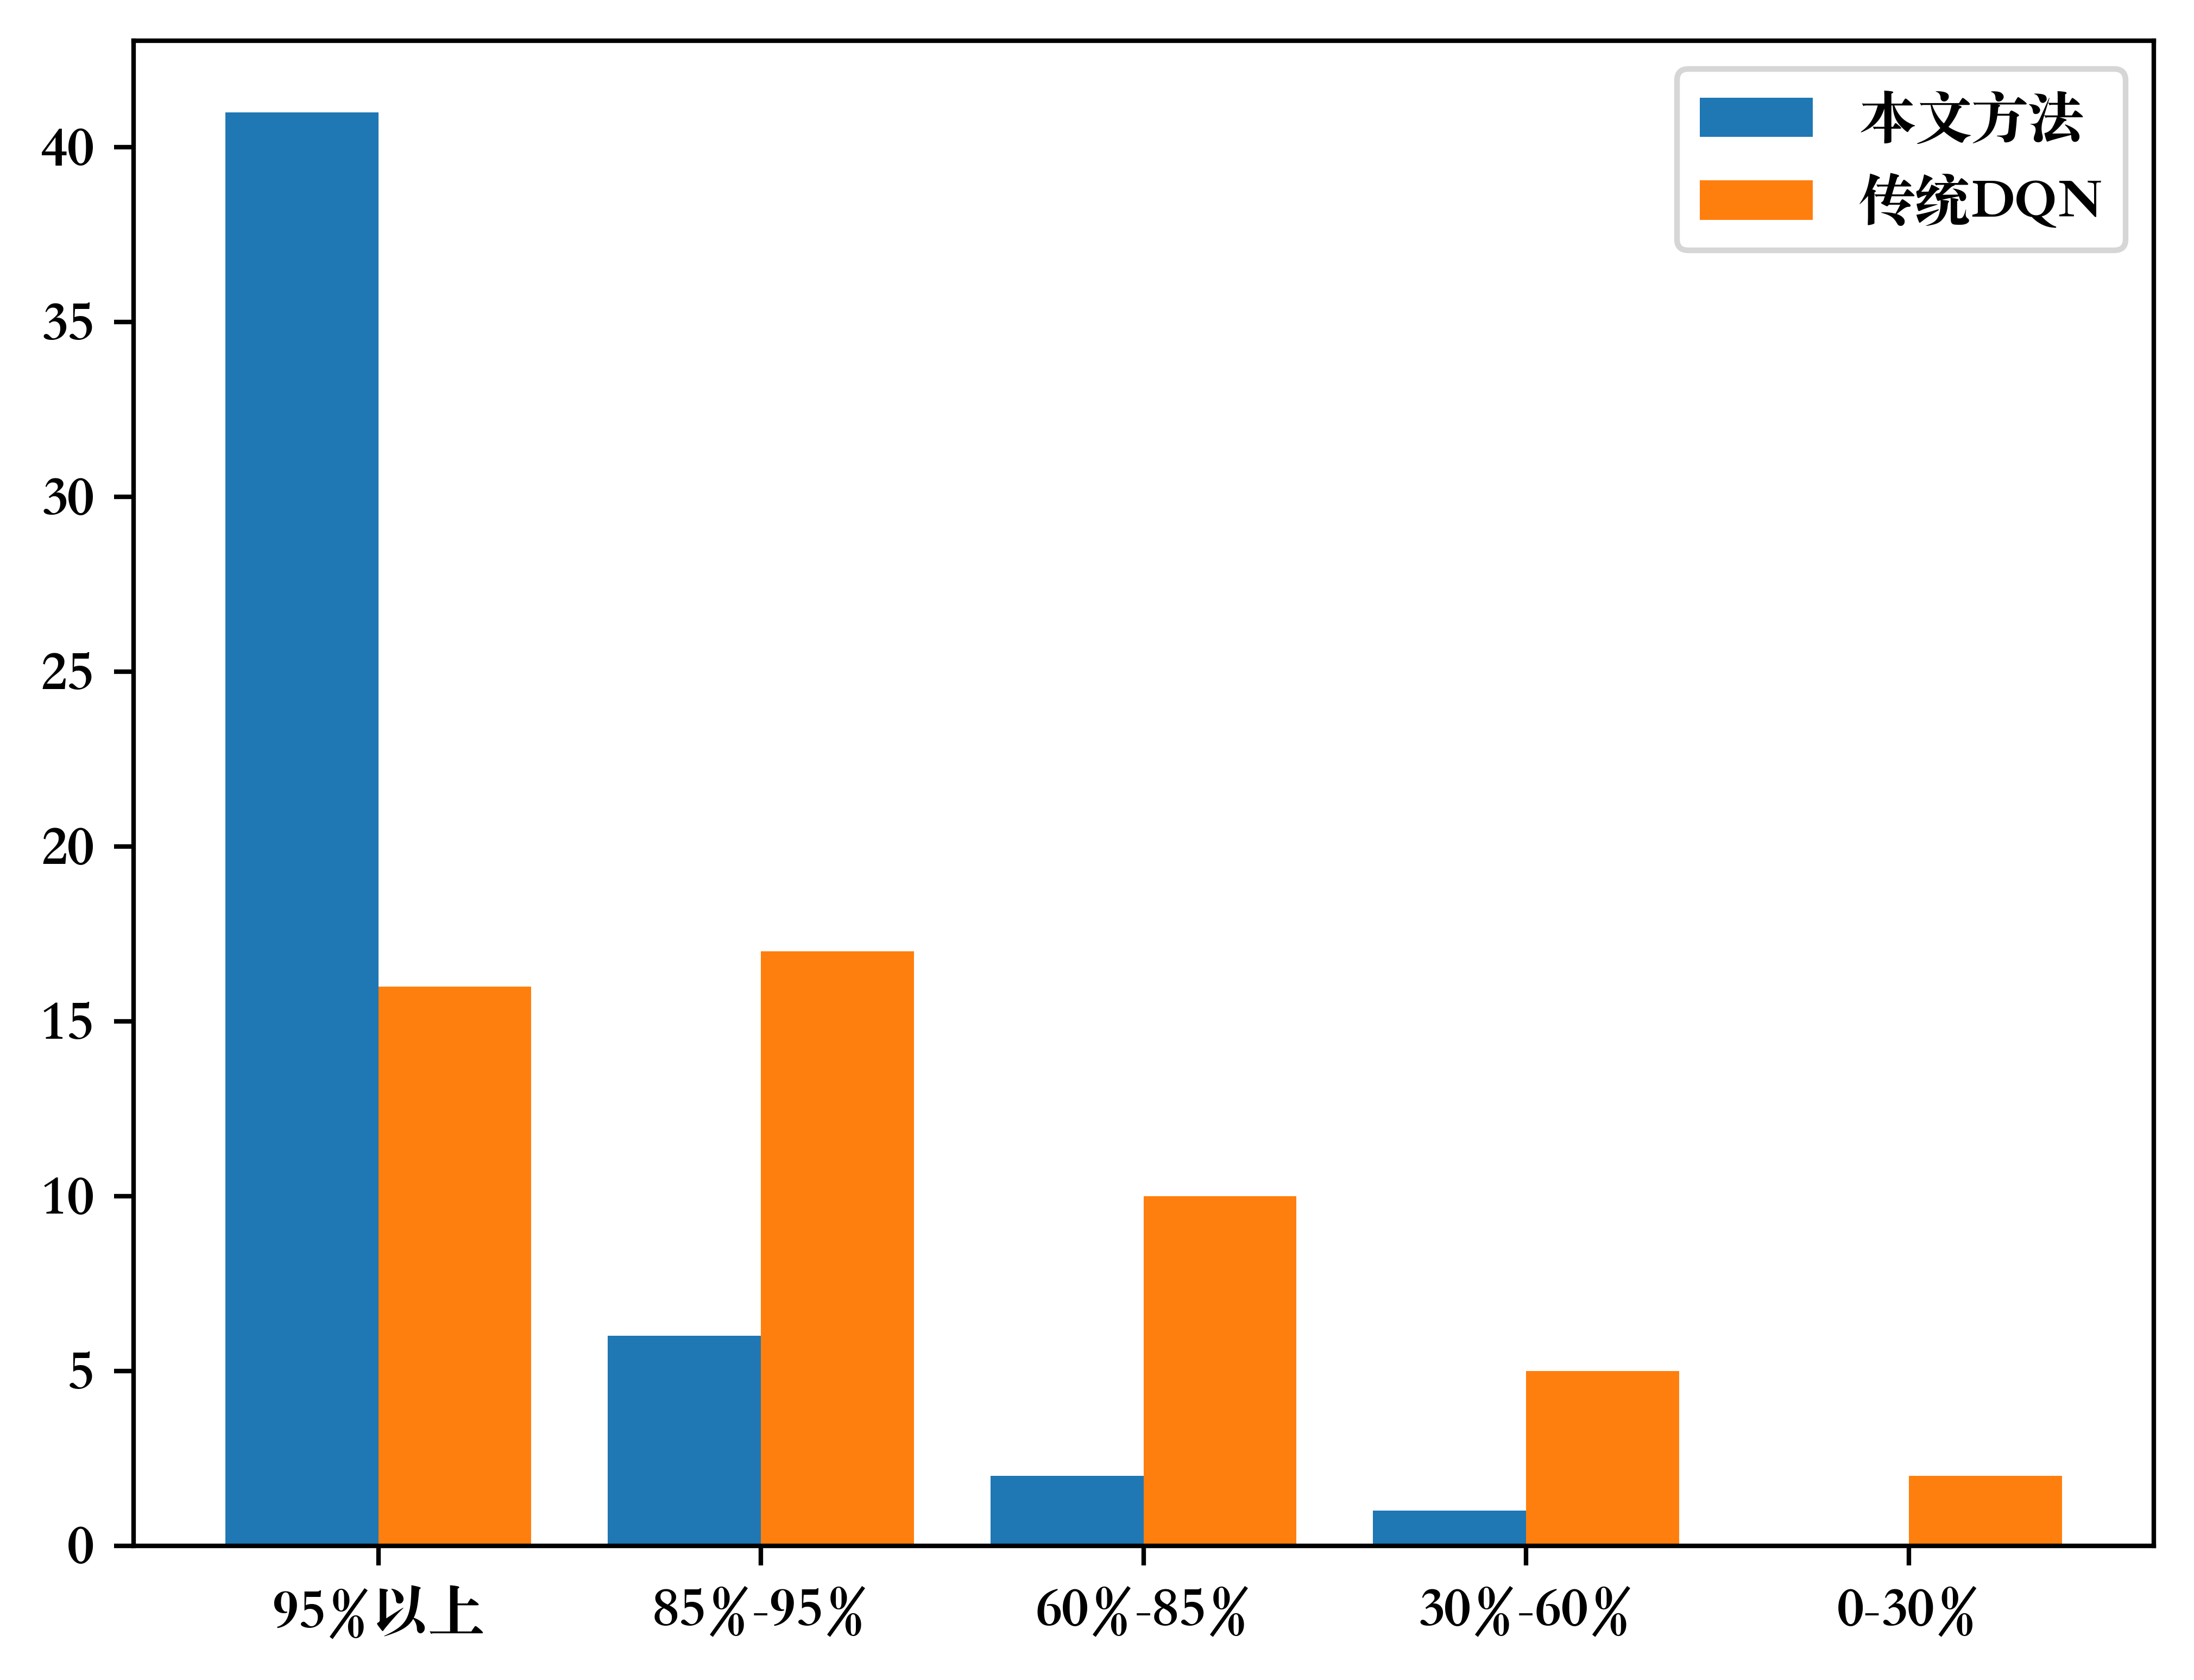
\includegraphics[width=.5\textwidth]{figures/content/com4.png}}
  \caption{选定测试个体的性能比较以及与朴素法最大奖励值的比较}
  \label{com}
\end{figure}

在本次实验中,随机选取了一部分个体,并将其用作测试集。然后,对这些测试集中的个体进行了测试,并计算了它们的平均奖励值。结果表明,测试集中的个体的表现略低于训练集中的个体,但仍表现出较好的性能。这表明所提出的方法具有一定的泛化能力,即能够适应一些新的情况并产生有意义的结果。


\subsection{部分信息感知的模型检验}

在现实世界中,人们在做出决策时,通常不会拥有完全的信息,例如,可能无法准确地了解周围环境、其他人的行为、交通状况等。因此,仅仅依靠部分信息进行决策,可能会导致更差的行动选择。为了比较所提出的深度强化学习方法的性能,此小节引入了另外两种模型,以考虑在部分信息的情况下,深度强化学习方法是否仍然是有效的。

第一个是一阶马尔可夫链(MC)模型,仅使用当前旅行距离和出发时间差来决定下一个选择。其状态、转移和初始状态概率以及奖励函数均源自DRL模型。两者的主要区别在于决策过程。MC模型使用转移和初始状态概率来模拟随时间变化的行为,而深度强化学习模型使用迭代试错过程。在一阶马尔可夫链(MC)模型中,每个时间步都可以看作是一个状态,用$s_t$表示。模型假设,行为只取决于当前状态$s_t$,并且在状态$s_t$下,采取行动$a_t$会以概率$p(s_{t+1}|s_t, a_t)$转移到下一个状态$s_{t+1}$,其中$p(s_{t+1}|s_t, a_t)$表示在状态$s_t$下采取行动$a_t$并转移到状态$s_{t+1}$的概率。这个概率可以通过训练数据中的频率来估计。另外,MC模型还需要一个初始状态分布$\mu$,表示在开始时每个状态的出现概率。这个分布也可以通过训练数据中的频率来估计。在决策过程中,MC模型首先从初始状态分布$\mu$中随机选取一个初始状态$s_0$。然后,在每个时间步$t$,根据当前状态$s_t$和行动$a_t$,使用转移概率$p(s_{t+1}|s_t, a_t)$随机转移到下一个状态$s_{t+1}$。在每个时间步,根据当前状态$s_t$和一些其他信息(例如旅行时间,距离等),MC模型使用某种规则(例如贪心算法)选择下一个行动$a_t$,直到终止状态被达到。相比之下,深度强化学习方法不仅使用状态和行动,还使用神经网络来学习状态和行动之间的复杂映射关系,并使用Q值函数来指导行动选择。因此,深度强化学习方法具有更好的表达能力和泛化能力,可以更好地处理具有大量状态和行动的环境。

第二个是传统的MNL模型,传统的MNL模型是基于多项式逻辑回归的经典模型,它用于预测个体选择某个行动的概率。MNL模型通常使用可解释的特征来描述选择行动的动机。这些特征通常是人为选择的,而不是通过学习过程得到的。例如,特征可能包括行动的属性(如价格、距离、时间等),个体的属性(如性别、年龄、收入等)等。在本文中,用于对比的MNL模型使用深度强化学习的奖励函数作为效用函数。这里的奖励函数(式(\ref{reward function}))考虑了行动的成本和收益,通过计算收益与成本的比值得到奖励。

使用前文中在信息完全的情况下,由提出的方法得到的个体出行选择作为基准线,根据其来比较其他模型的性能。考虑了三个性能评估和比较指标。除了奖励值之外,另外两个是负对数损失(NLL)和Jaccard指数。NLL通常用于评估分类任务中的模型性能,特别是在类别不平衡的情况下。在本文中,使用NLL作为评价指标,可以测量每种模型的预测能力,即它们在给定历史信息的情况下是否能够正确地预测个体的行动选择。NLL的较低值表示模型更准确地预测了行动选择,因此较低的NLL值是期望的。Jaccard指数是一种测量相似性的指标。在本文中,它可以测量每个模型产生的行动选择与基准线之间的相似程度。基准线是在信息完全的情况下,由提出的方法得到的个体出行选择。因此,Jaccard指数可以反映其他模型相对于基线的优化水平。值越高表示其他模型的行动选择越接近基线,因此较高的Jaccard指数是期望的。这两个指标都衡量其他模型产生的行动与基线获得的行动之间的接近程度或相似程度。因此,它们可以反映其他模型相对于基线的优化水平。

表\ref{tab:eva}中展示了三个性能指标的比较结果。正如预期的那样,在信息完全的情况下,所提出的方法表现出了最佳性能,可以获得尽可能多的奖励。相比之下,其他所有模型的性能都较差,这可以通过比较平均奖励值来看出,这些值都低于基线的奖励值,类似的趋势也反映在NLL和Jaccard指数上。然而,即使在部分信息的情况下,所提出的方法仍然表现出比一阶MC模型和MNL模型略好的性能,这表明所提出的方法即使在存在部分信息的情况下,仍然是有效的。

\begin{table}[htbp]
\centering
\caption{不同替代模型的性能评估结果}
\label{tab:eva}
\renewcommand{\arraystretch}{1.2} % 使表格行间距加大1.2倍
\setlength{\tabcolsep}{8mm} % 设置表格列间距为8mm
\small % 设置表格字体大小为小号

\begin{tabular}{lccc}
\toprule
模型 & NLL & 平均回报 & 准确度 \\
\midrule
一阶MC模型 & 19.23 & 1,354 & 0.24 \\
MNL模型 & 24.17 & 1,217 & 0.23 \\
部分信息下的DRL方法 & 17.31 & 1,449 & 0.29 \\
完全信息下的DRL方法(基线) & \textbackslash{} & 1,735 & \textbackslash{} \\
\bottomrule
\end{tabular}
\end{table}

\subsection{模型参数的灵敏性分析}

为了探究本研究所提出的方法在模型参数变化时的性能变化,将进行两个敏感性分析。第一个参数是训练智能体数量的变化,第二个参数是训练个体的群组的选择。

为了探究前者的影响,在进一步的实验中,分别使用1、10、20和40个智能体进行训练。保持相同的实验设置,将60个个体的OD行程聚类成上述数字,并用另外50个测试个体则用于评估和比较。同样地,将朴素法作为参考进行比较。比较结果总结在表\ref{cluster_size}中。由于内存溢出,训练40个智能体的实验无法在本实验计算机上完成,因此没有报告结果。从表中可以看出,随着训练智能体数量的增加,所需的训练或计算时间增加,并且智能体数量的增加确实会导致更好的奖励。将一个智能体转变为四个智能体,奖励得到了最大的提高。进一步将该数字增加到10或20并不能显著提高奖励。这个结果表明,增加代表智能体数量相较于计算成本不一定合理。实际上,少量智能体已经可以在合理的计算时间内产生相当好的结果。使用朴素法得到的最大奖励作为参考值,比较所提出的方法所给出的奖励高于参考值95%以上的测试个体数量。如预期的那样,对于4、10和20个智能体,这个数字保持较大且变化很小。图\ref{agents}展示了对于不同数量的智能体,八个选定测试个体结果的比较。只有一个智能体显然不足以超过朴素法,而四个或更多智能体则有更良好的结果。

\begin{figure}[htbp]
  \subfloat{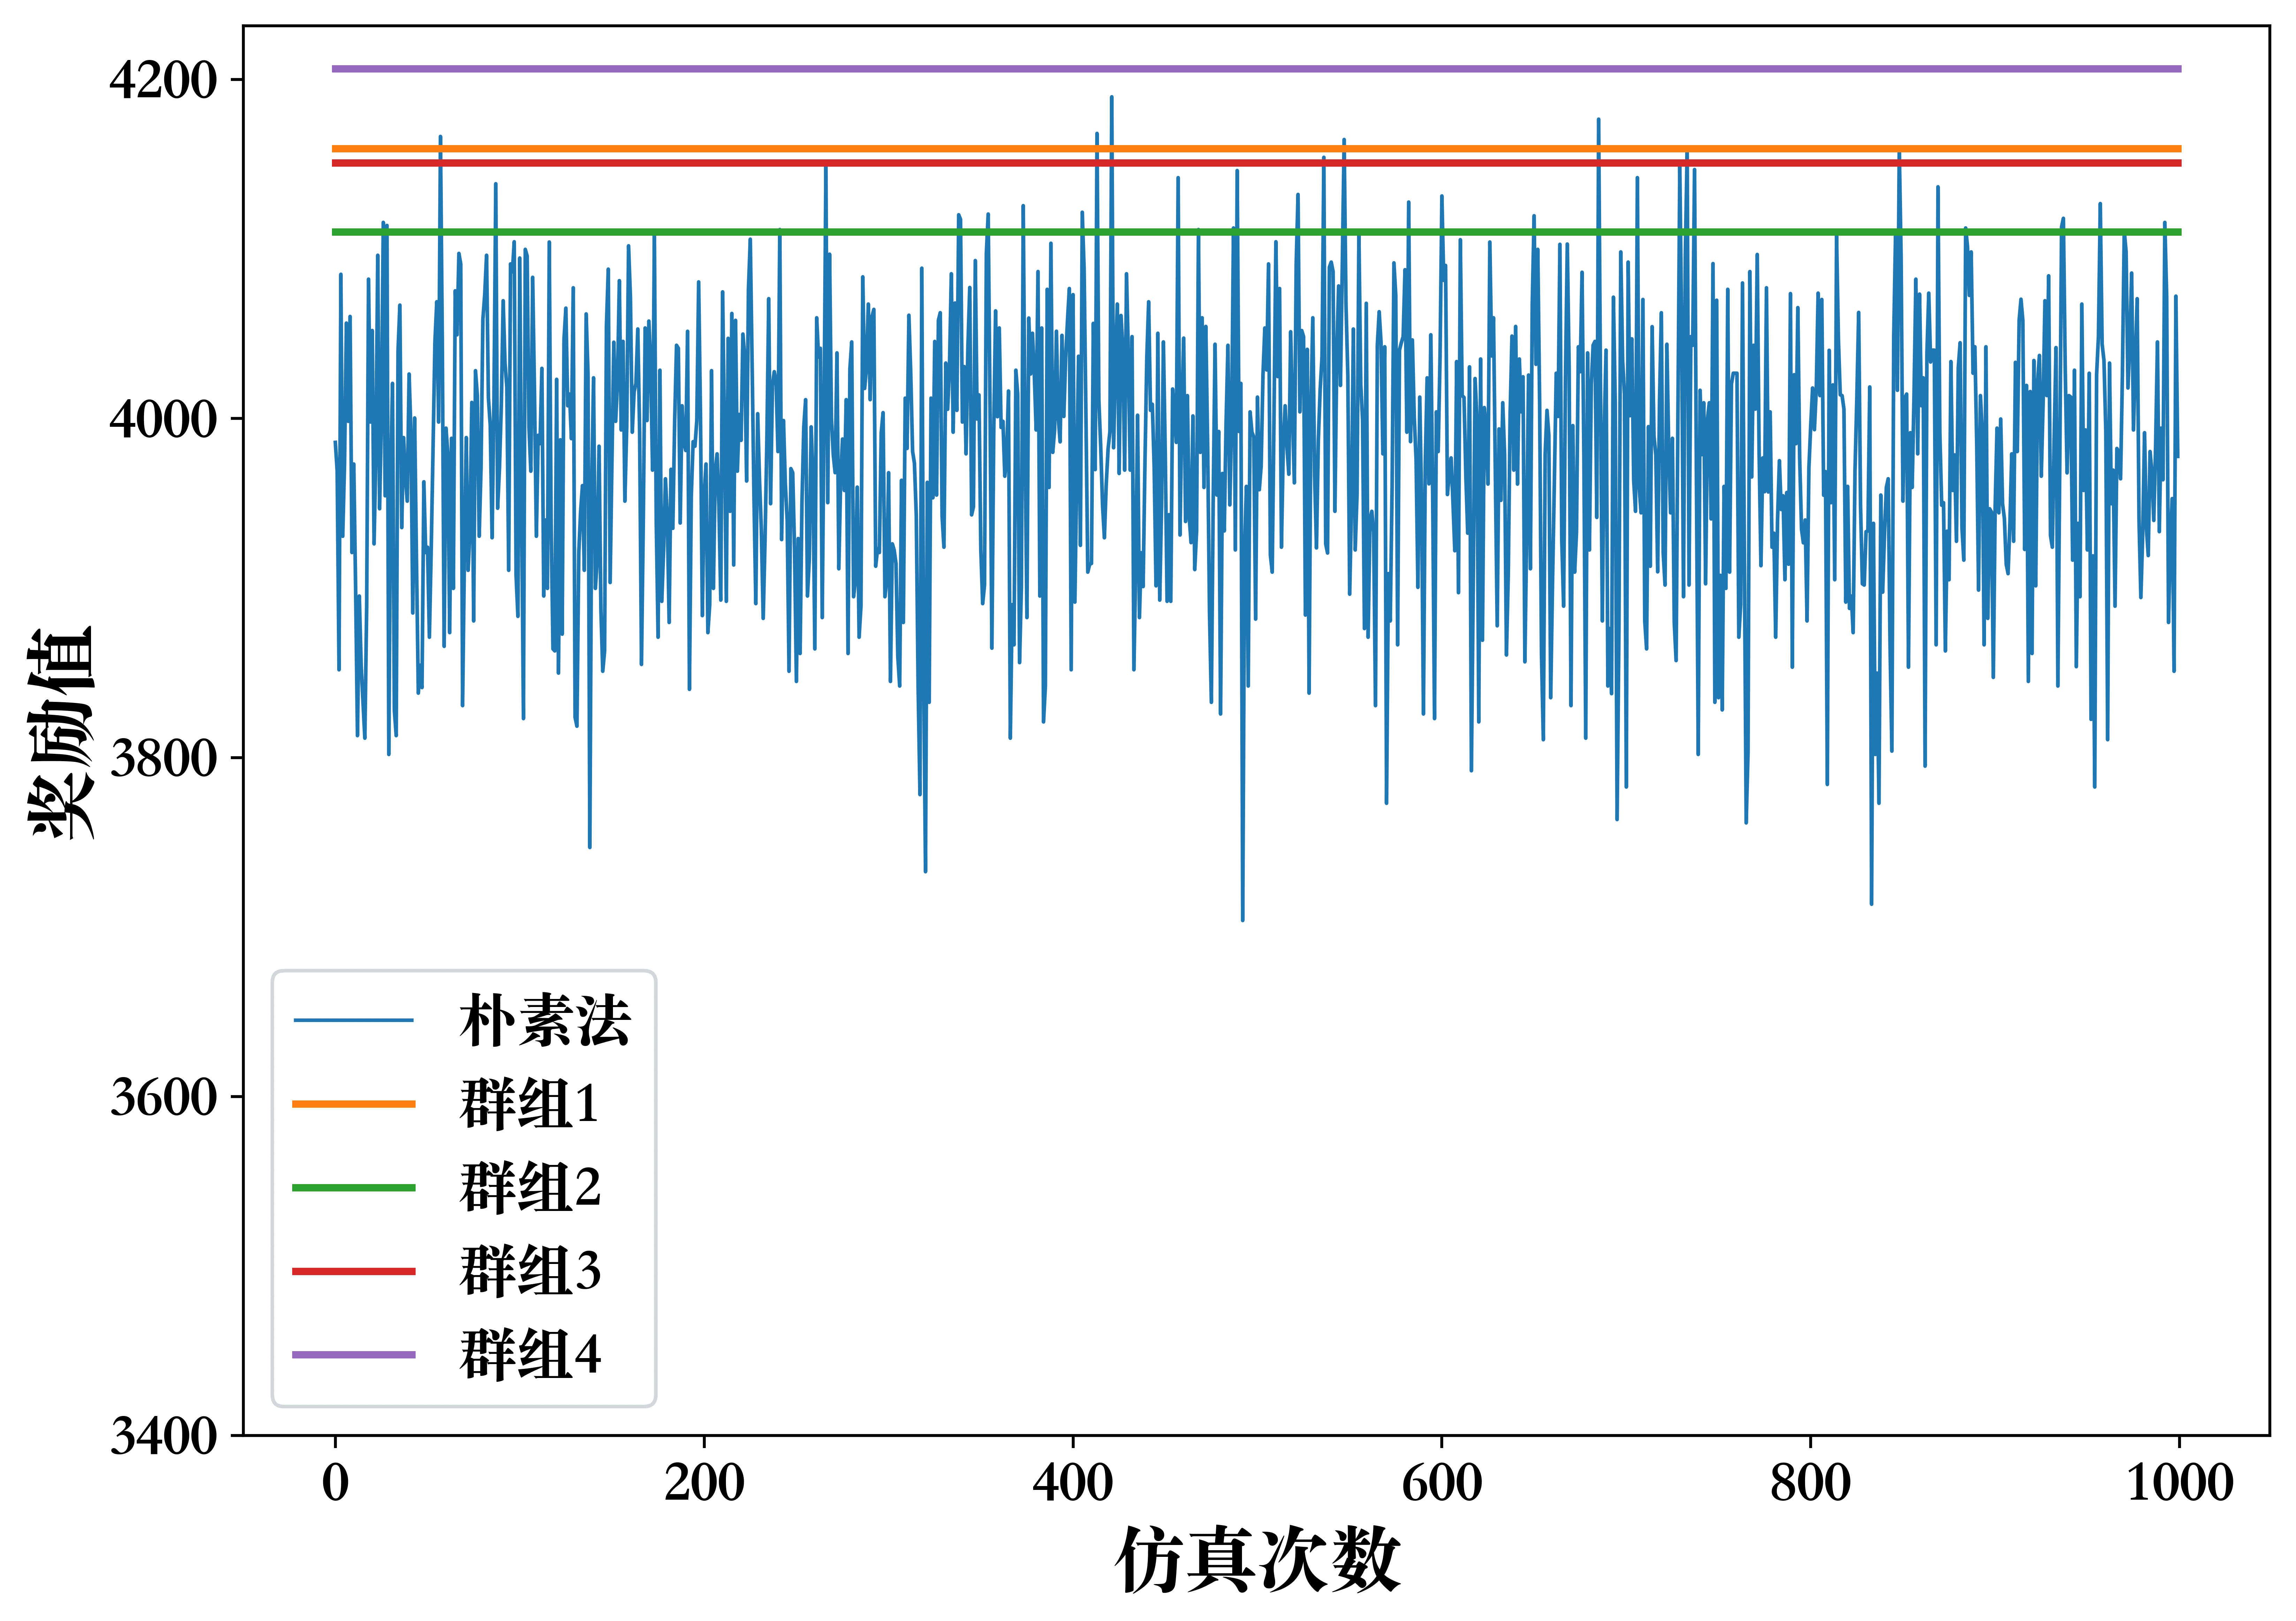
\includegraphics[width=.45\textwidth]{figures/content/agents/agent1.png}}
  \quad\quad
  \subfloat{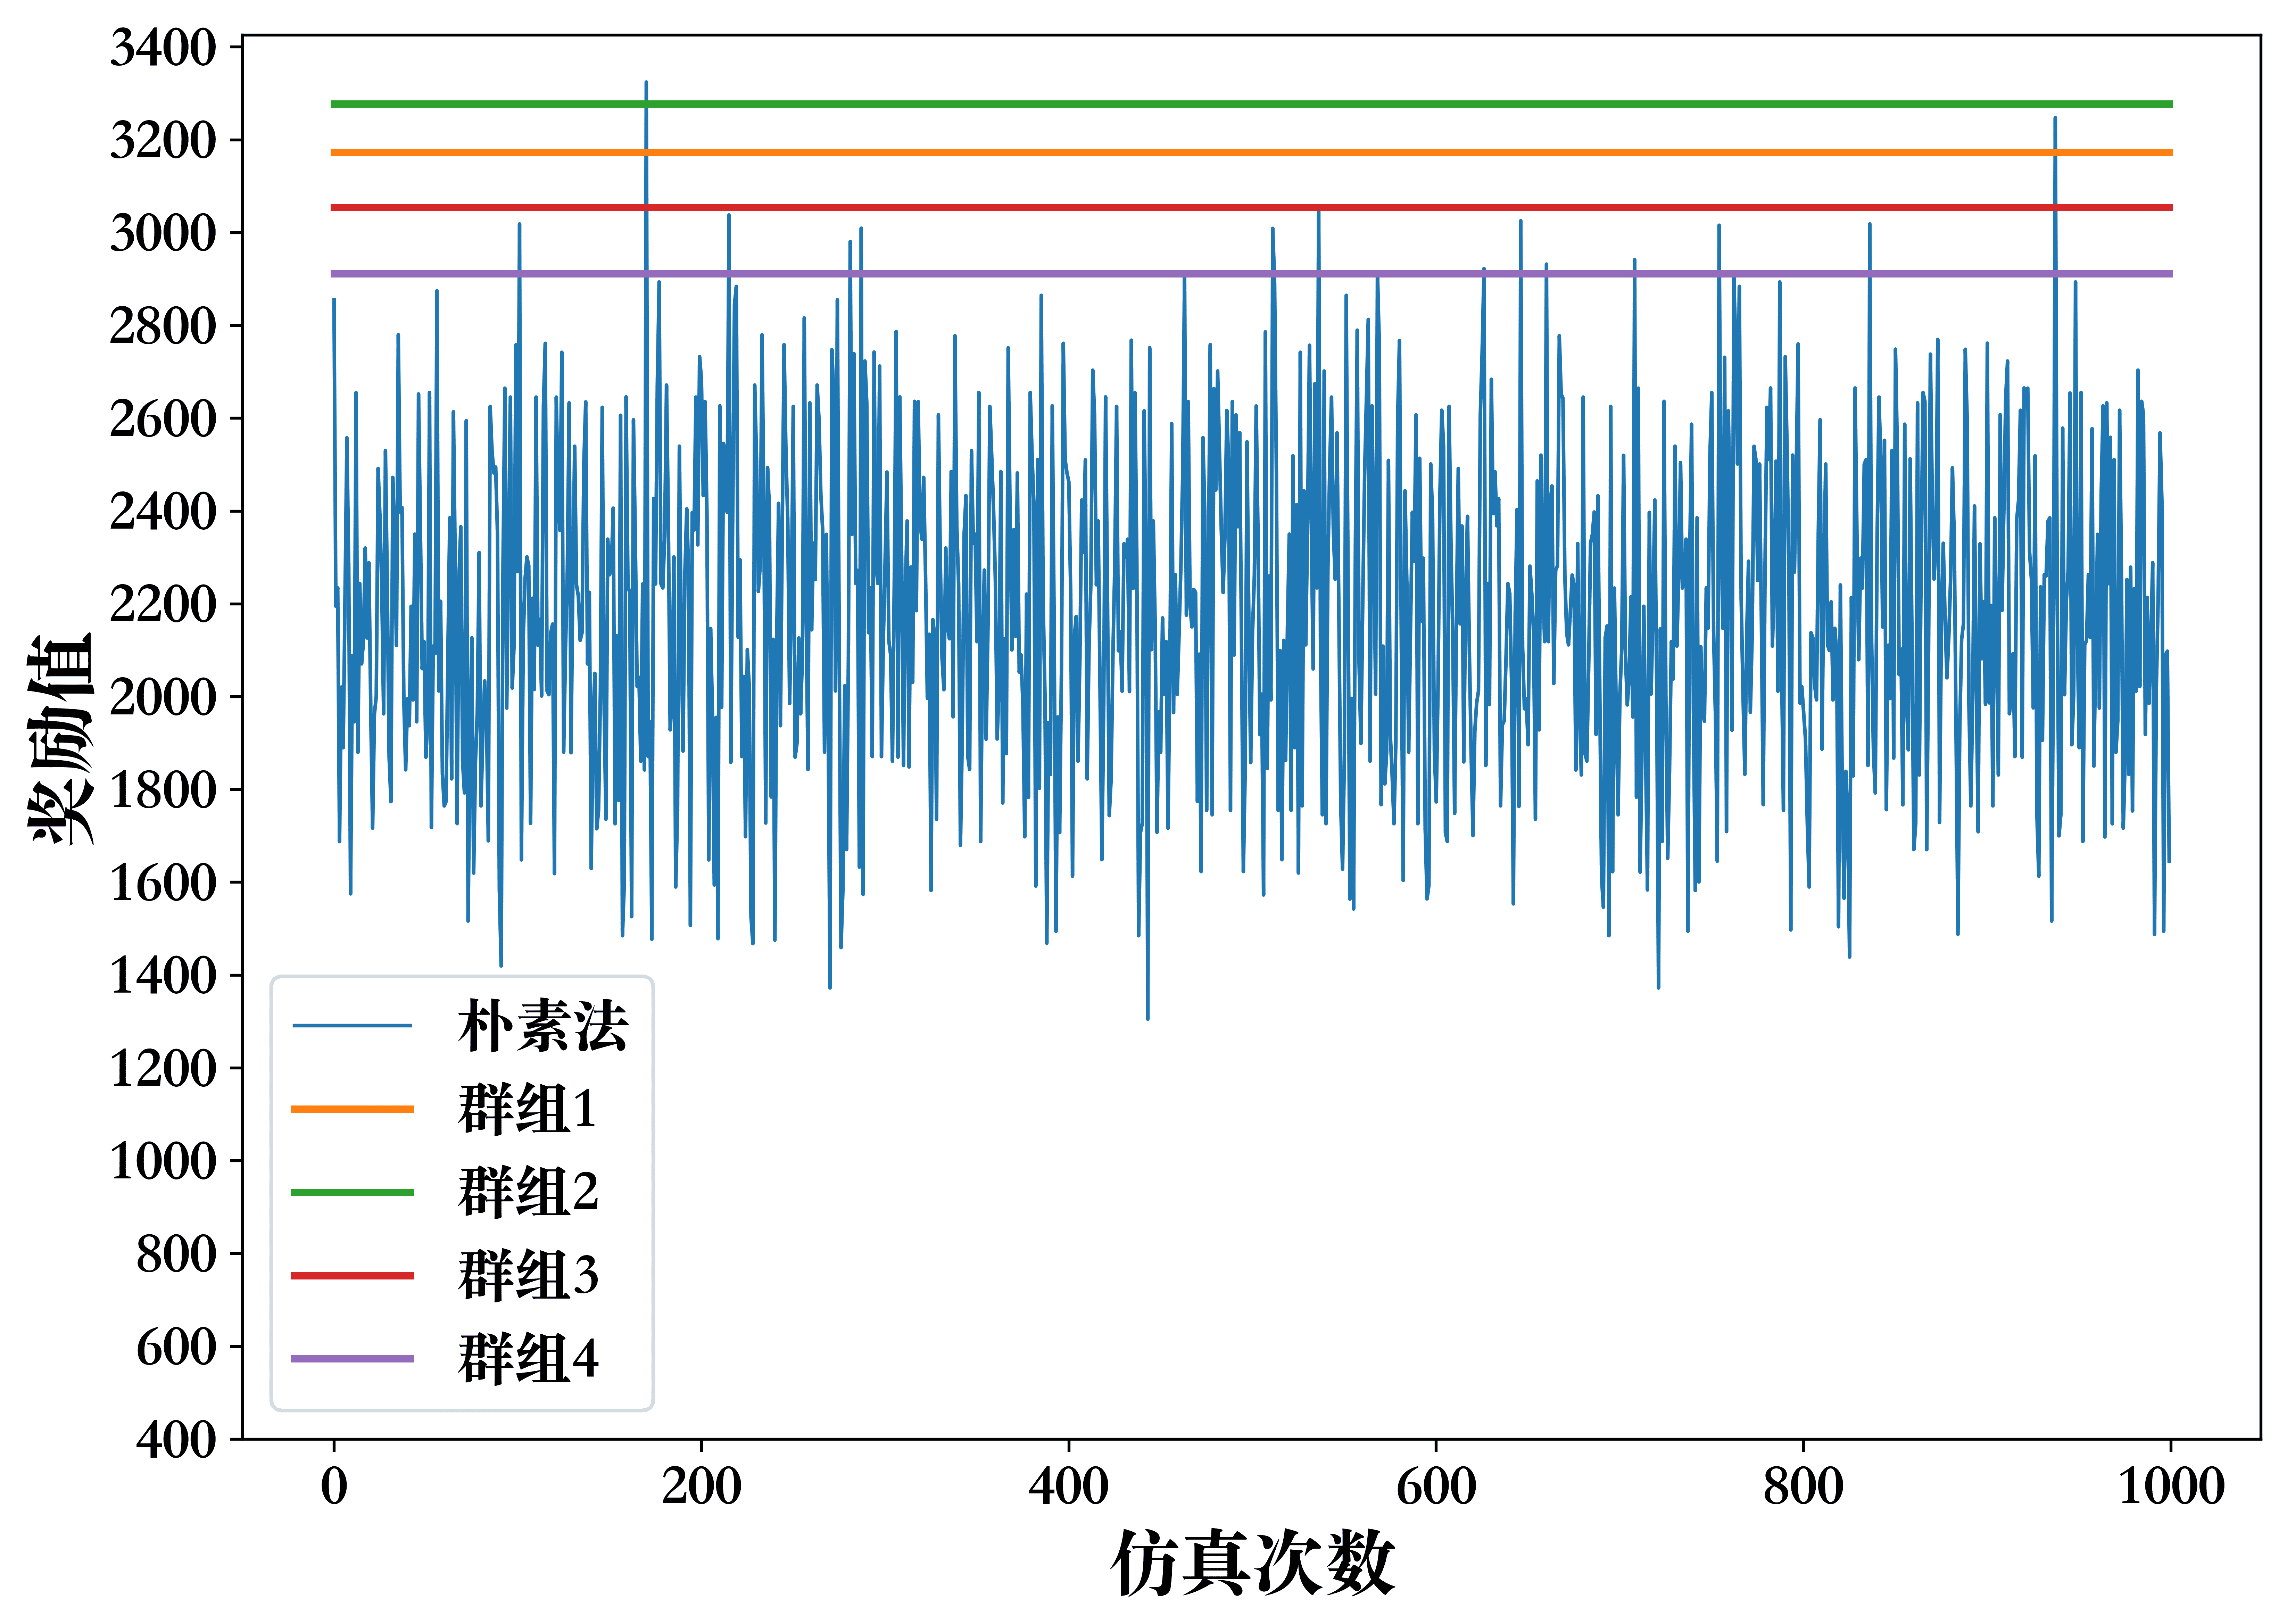
\includegraphics[width=.45\textwidth]{figures/content/agents/agent2.png}}
  \\
  \subfloat{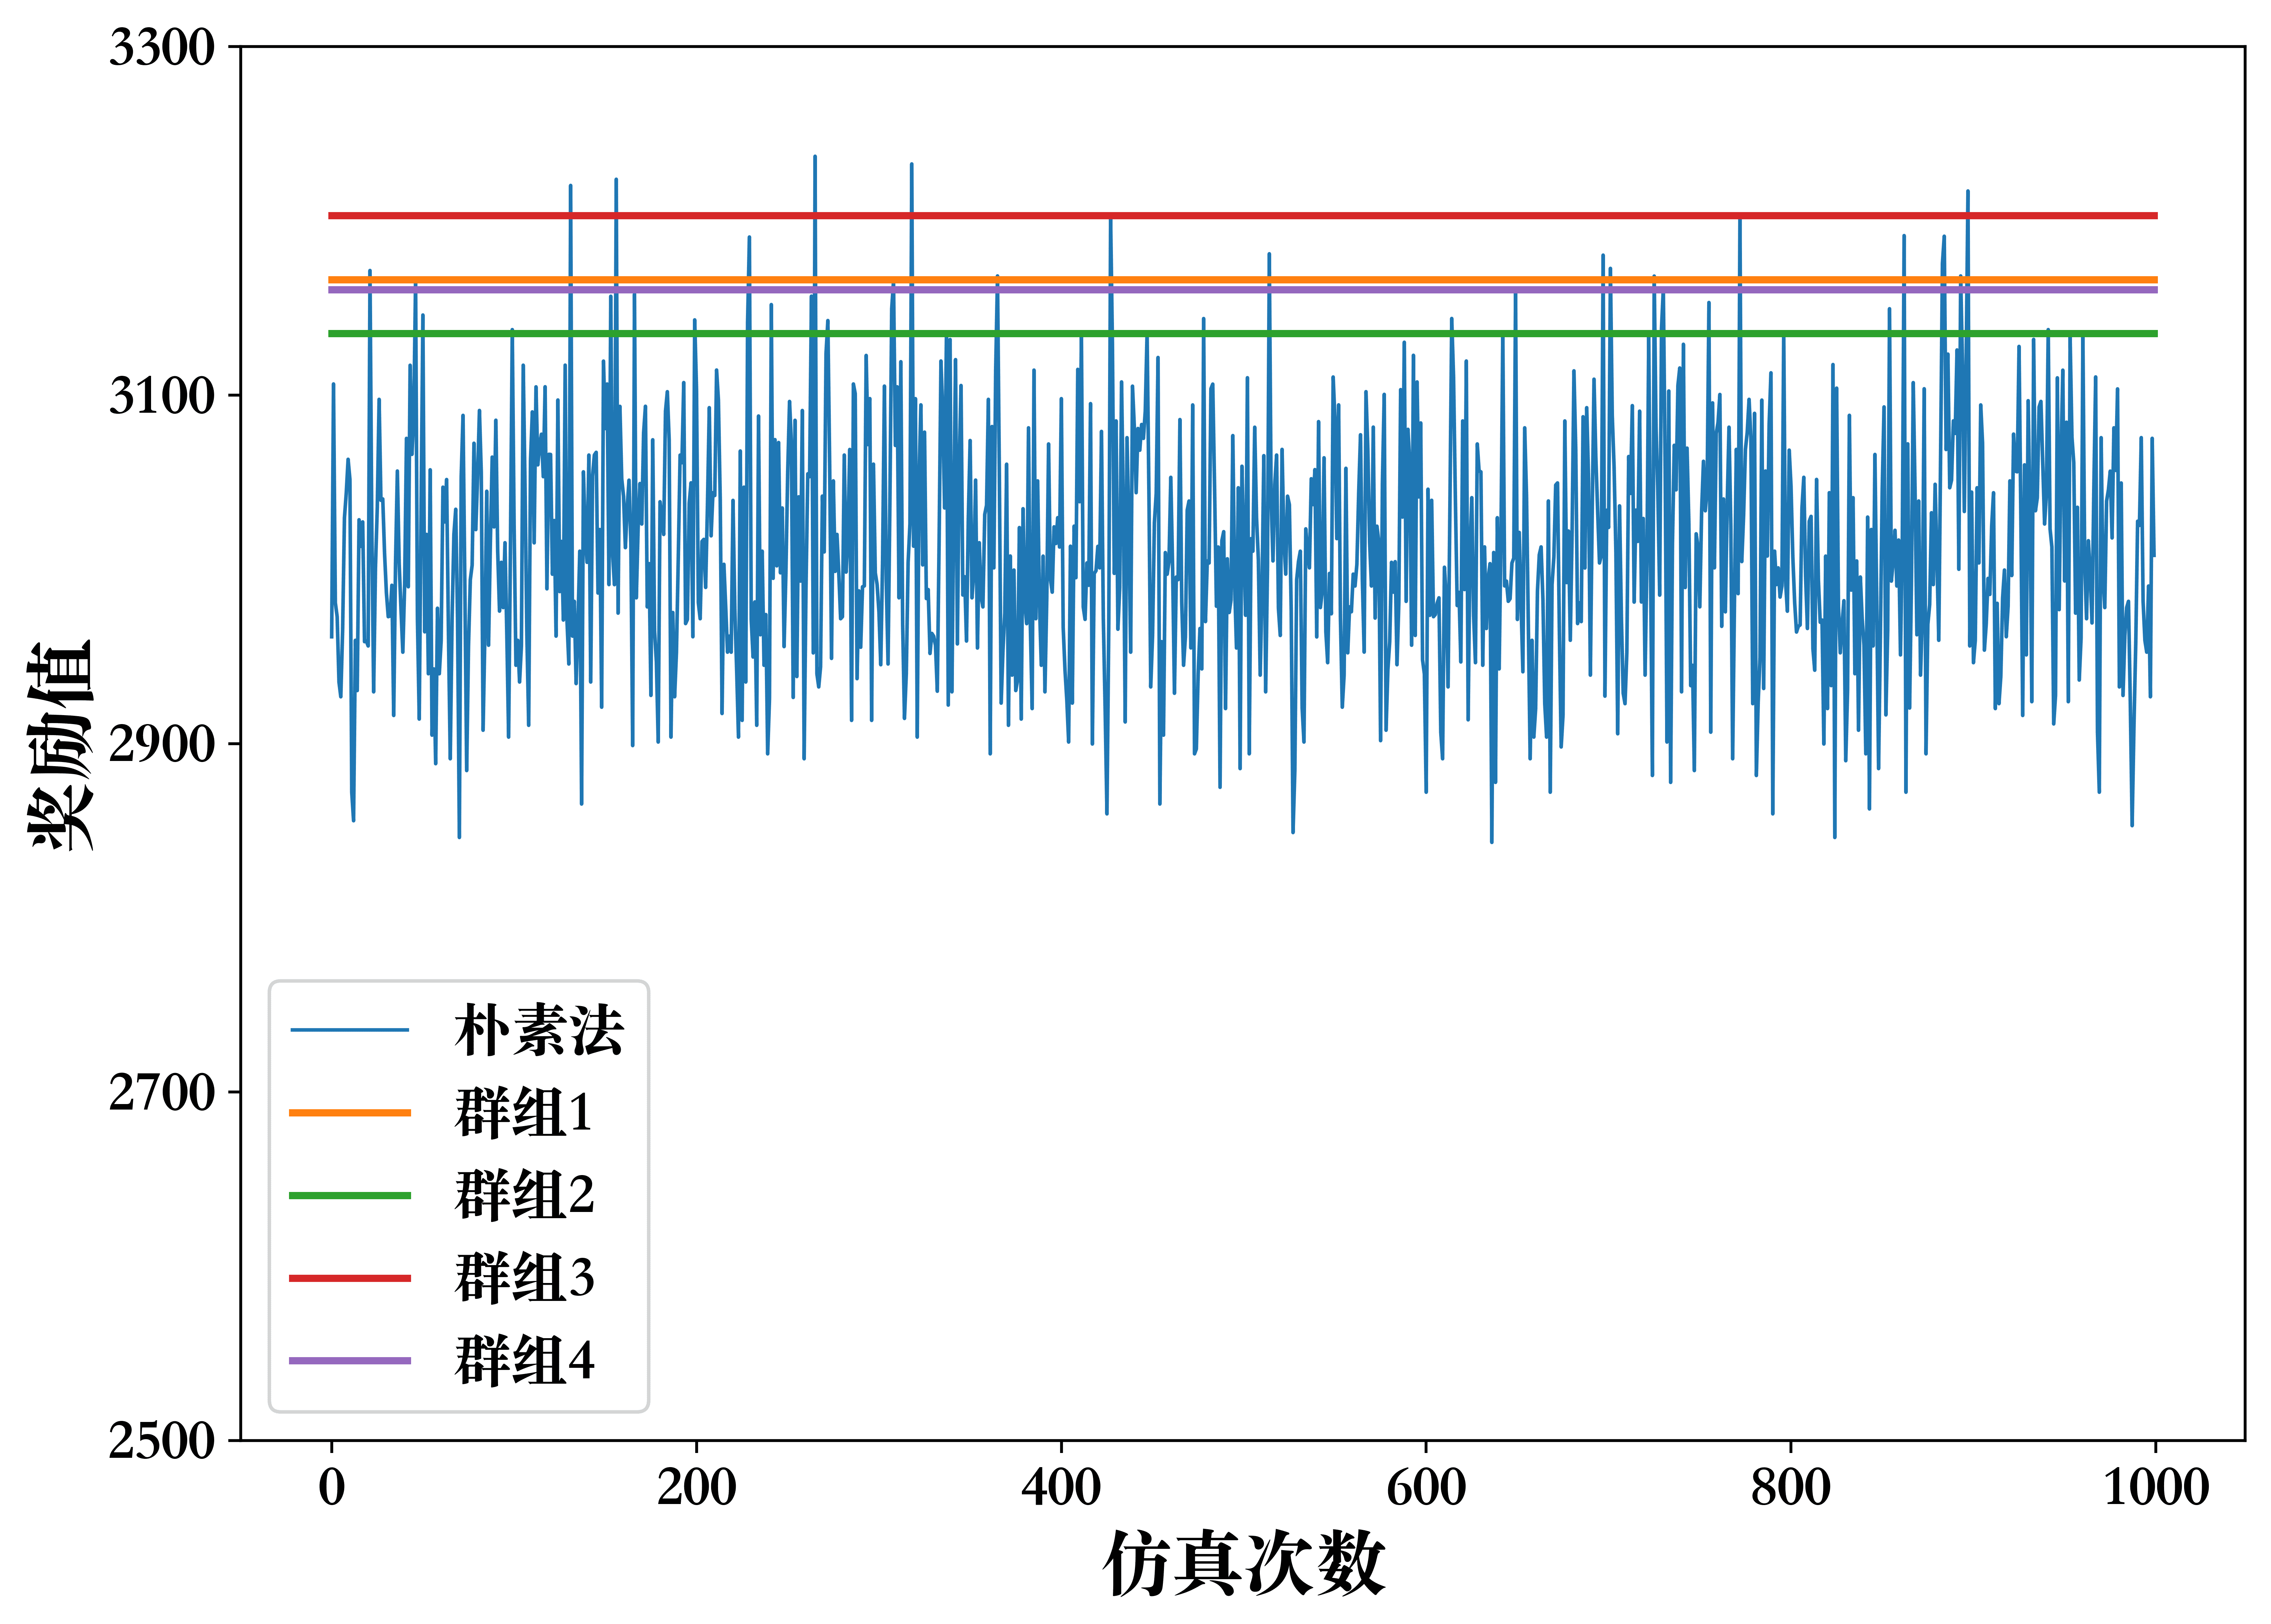
\includegraphics[width=.45\textwidth]{figures/content/agents/agent3.png}}
  \quad\quad
  \subfloat{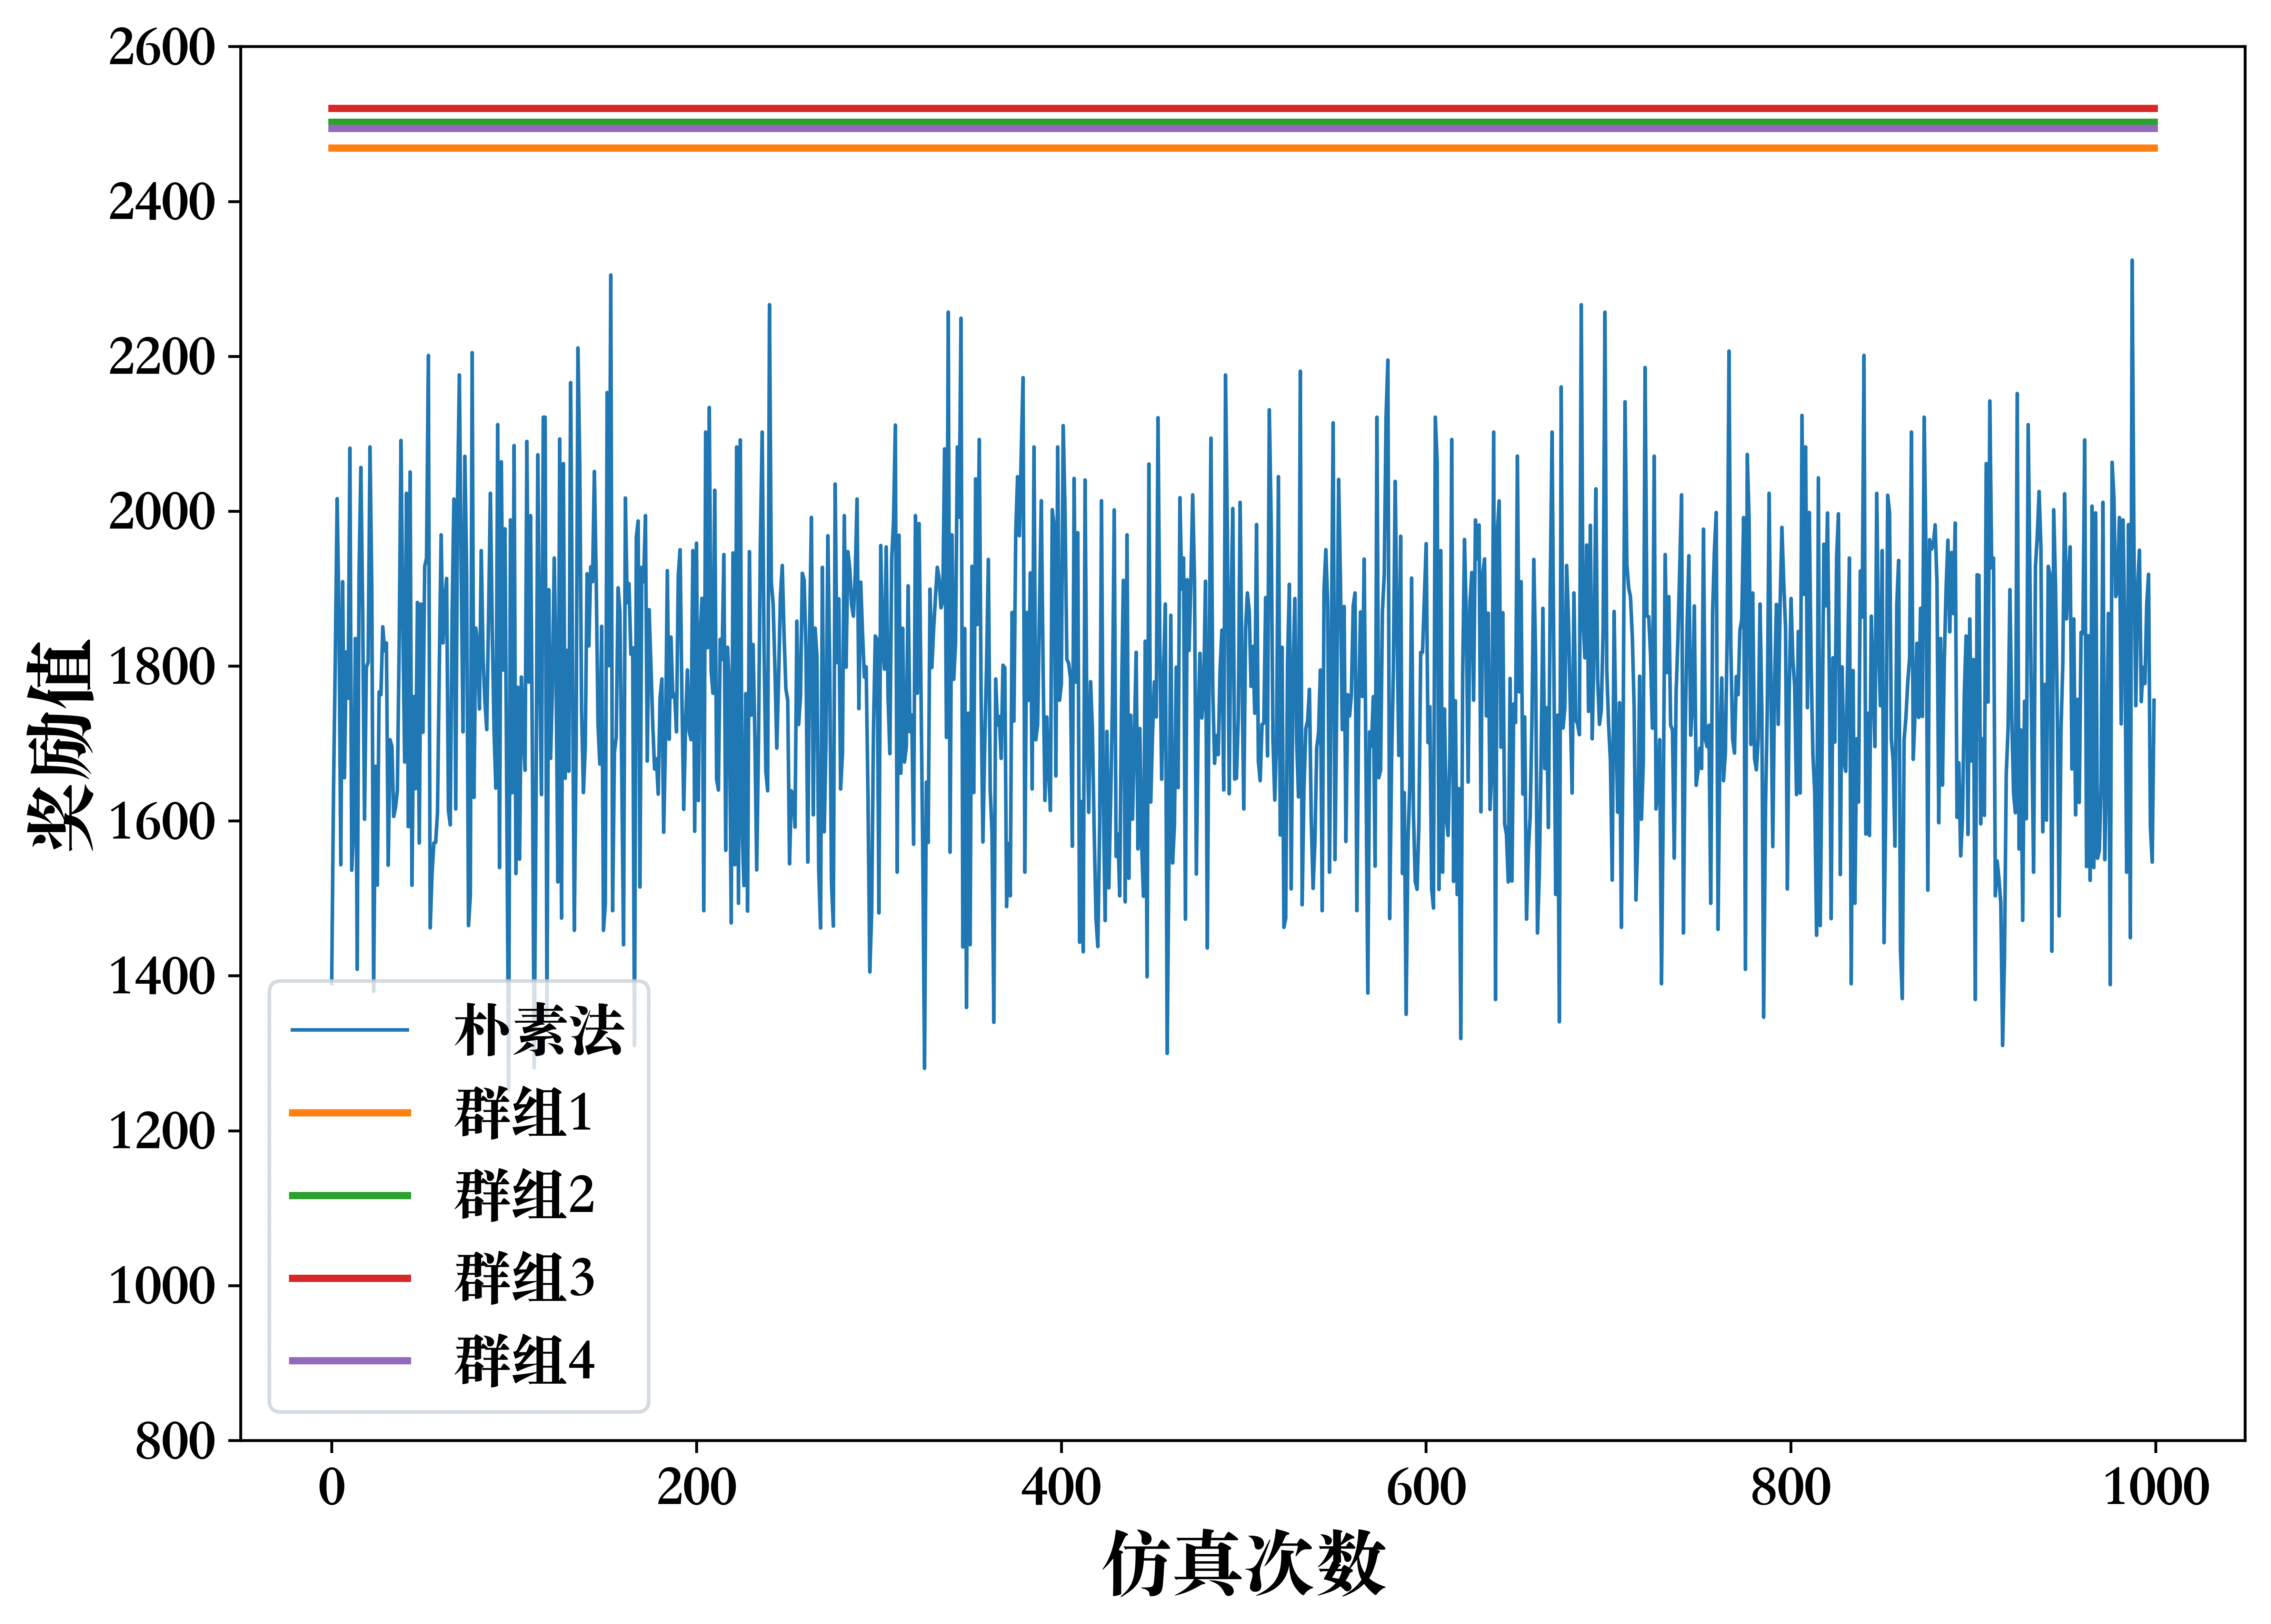
\includegraphics[width=.45\textwidth]{figures/content/agents/agent4.png}}
  \\
  \subfloat{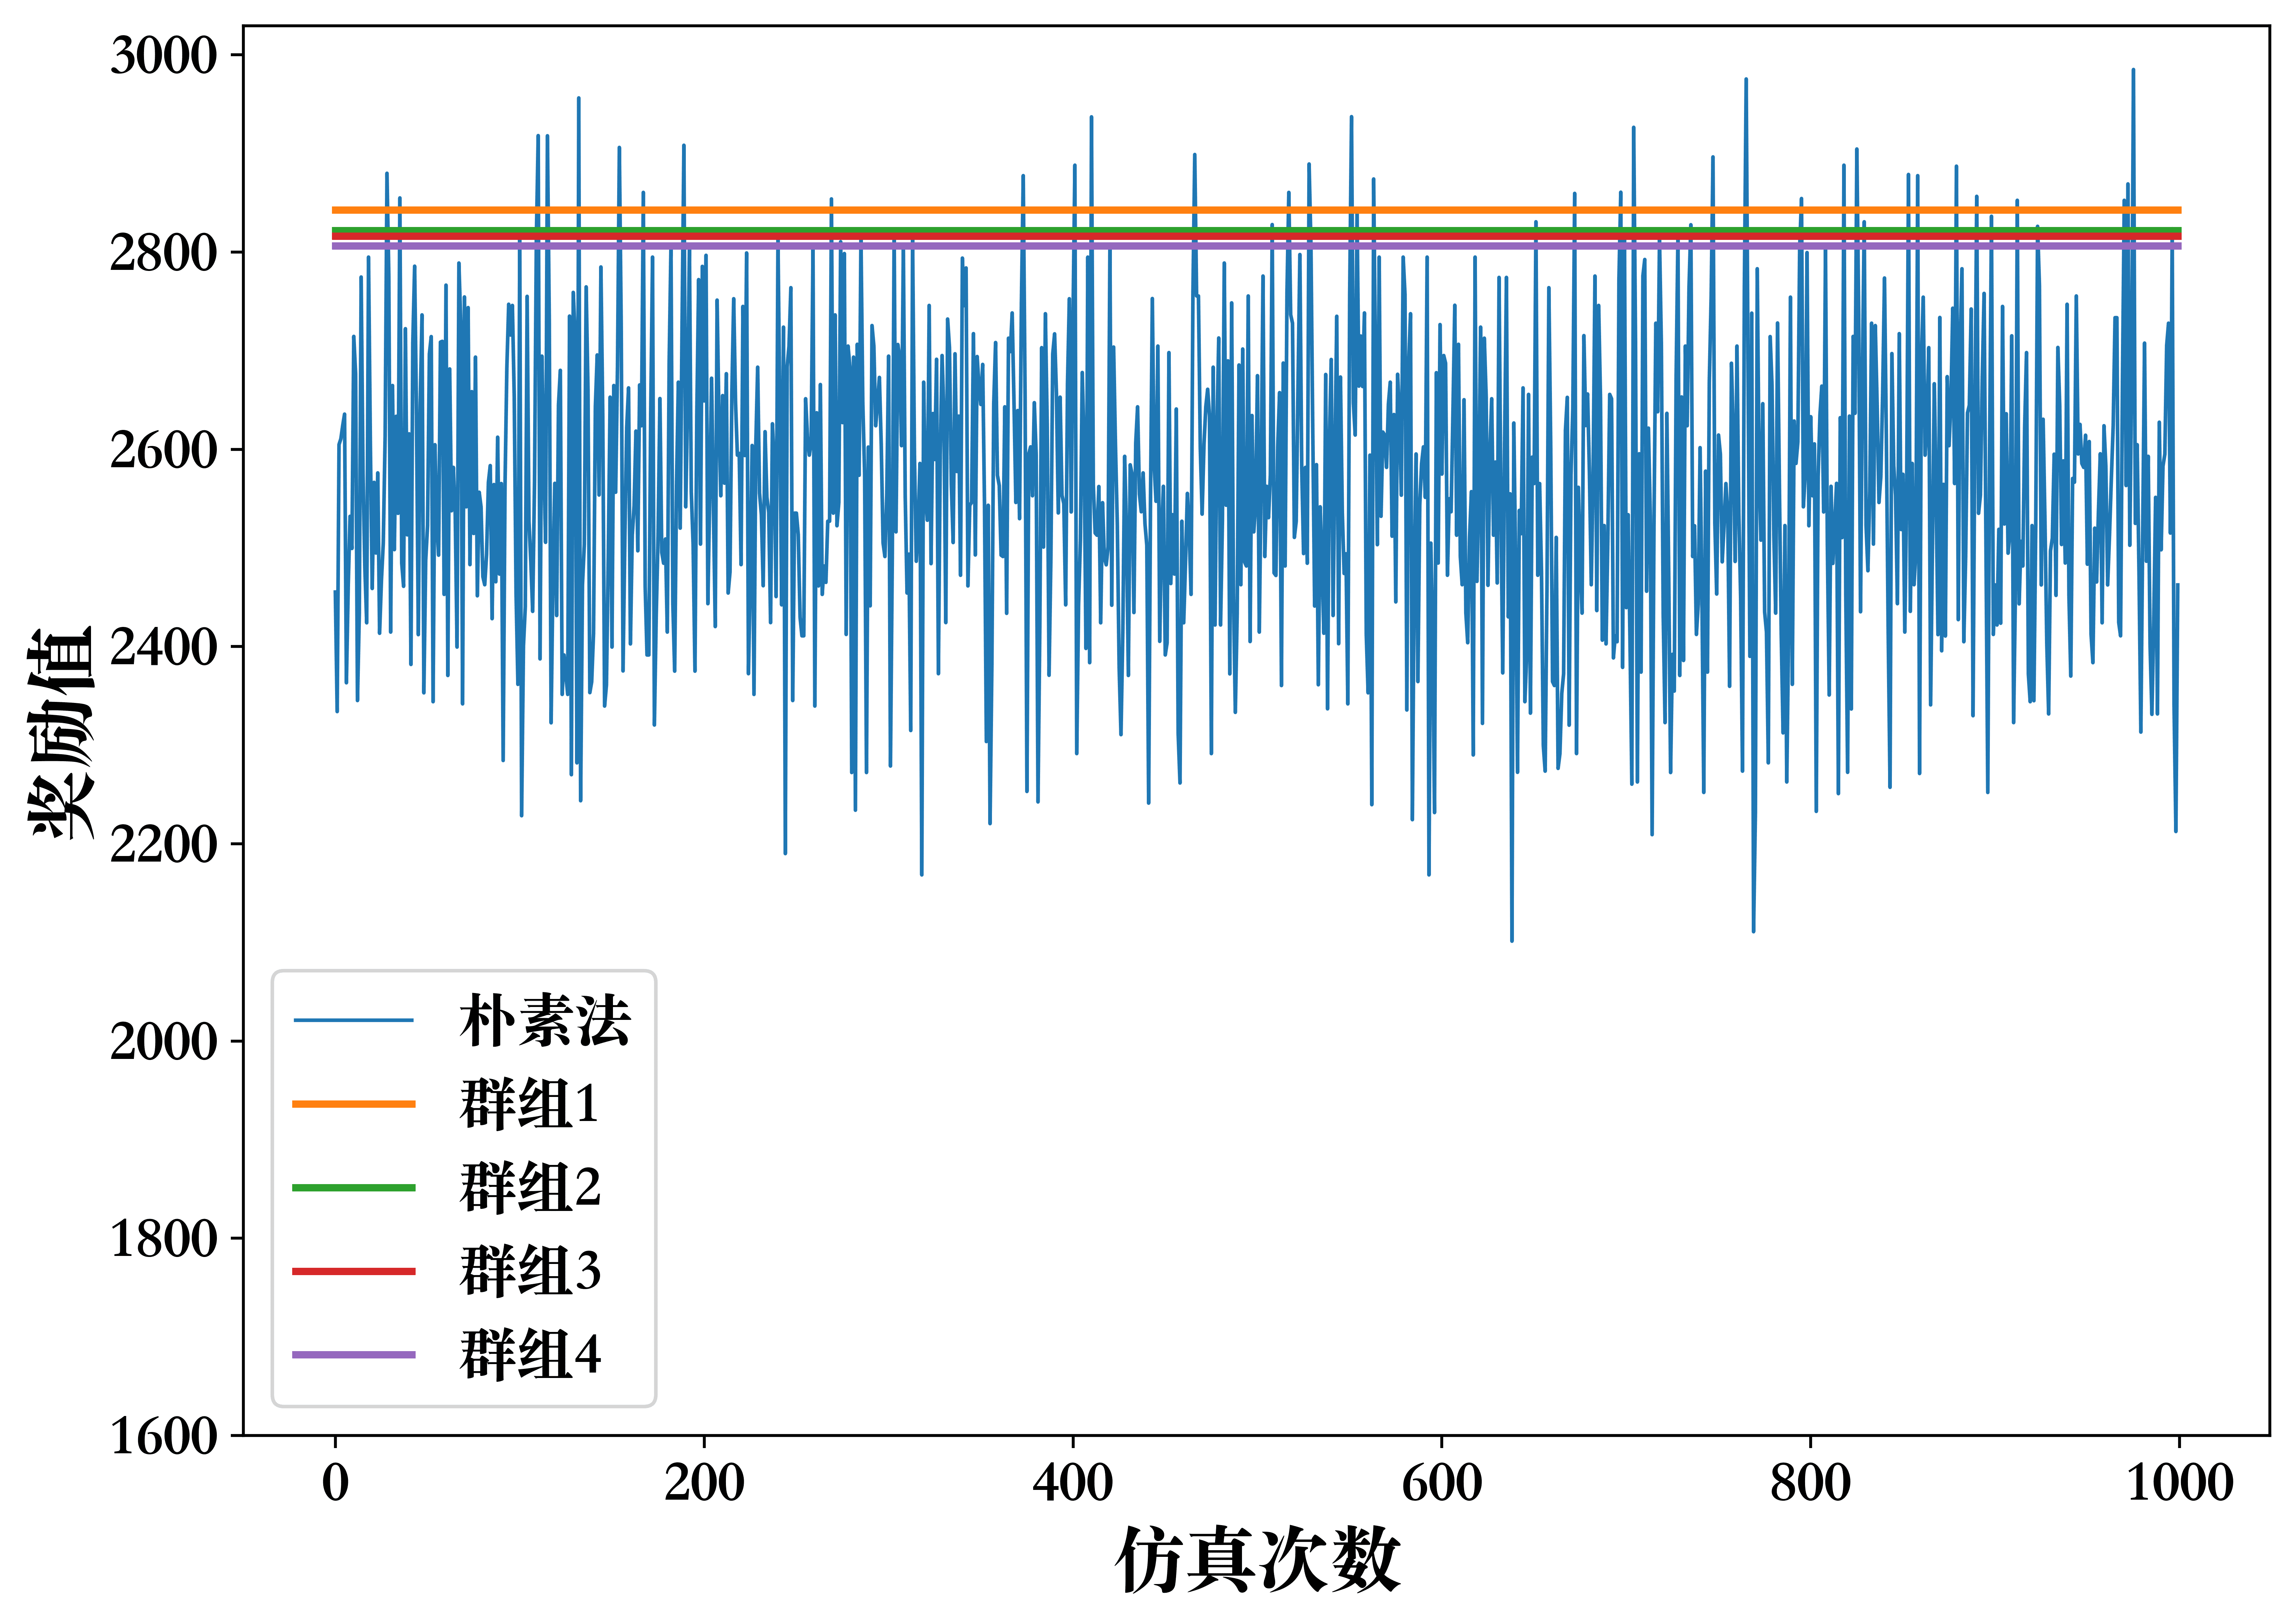
\includegraphics[width=.45\textwidth]{figures/content/agents/agent5.png}}
  \quad\quad
  \subfloat{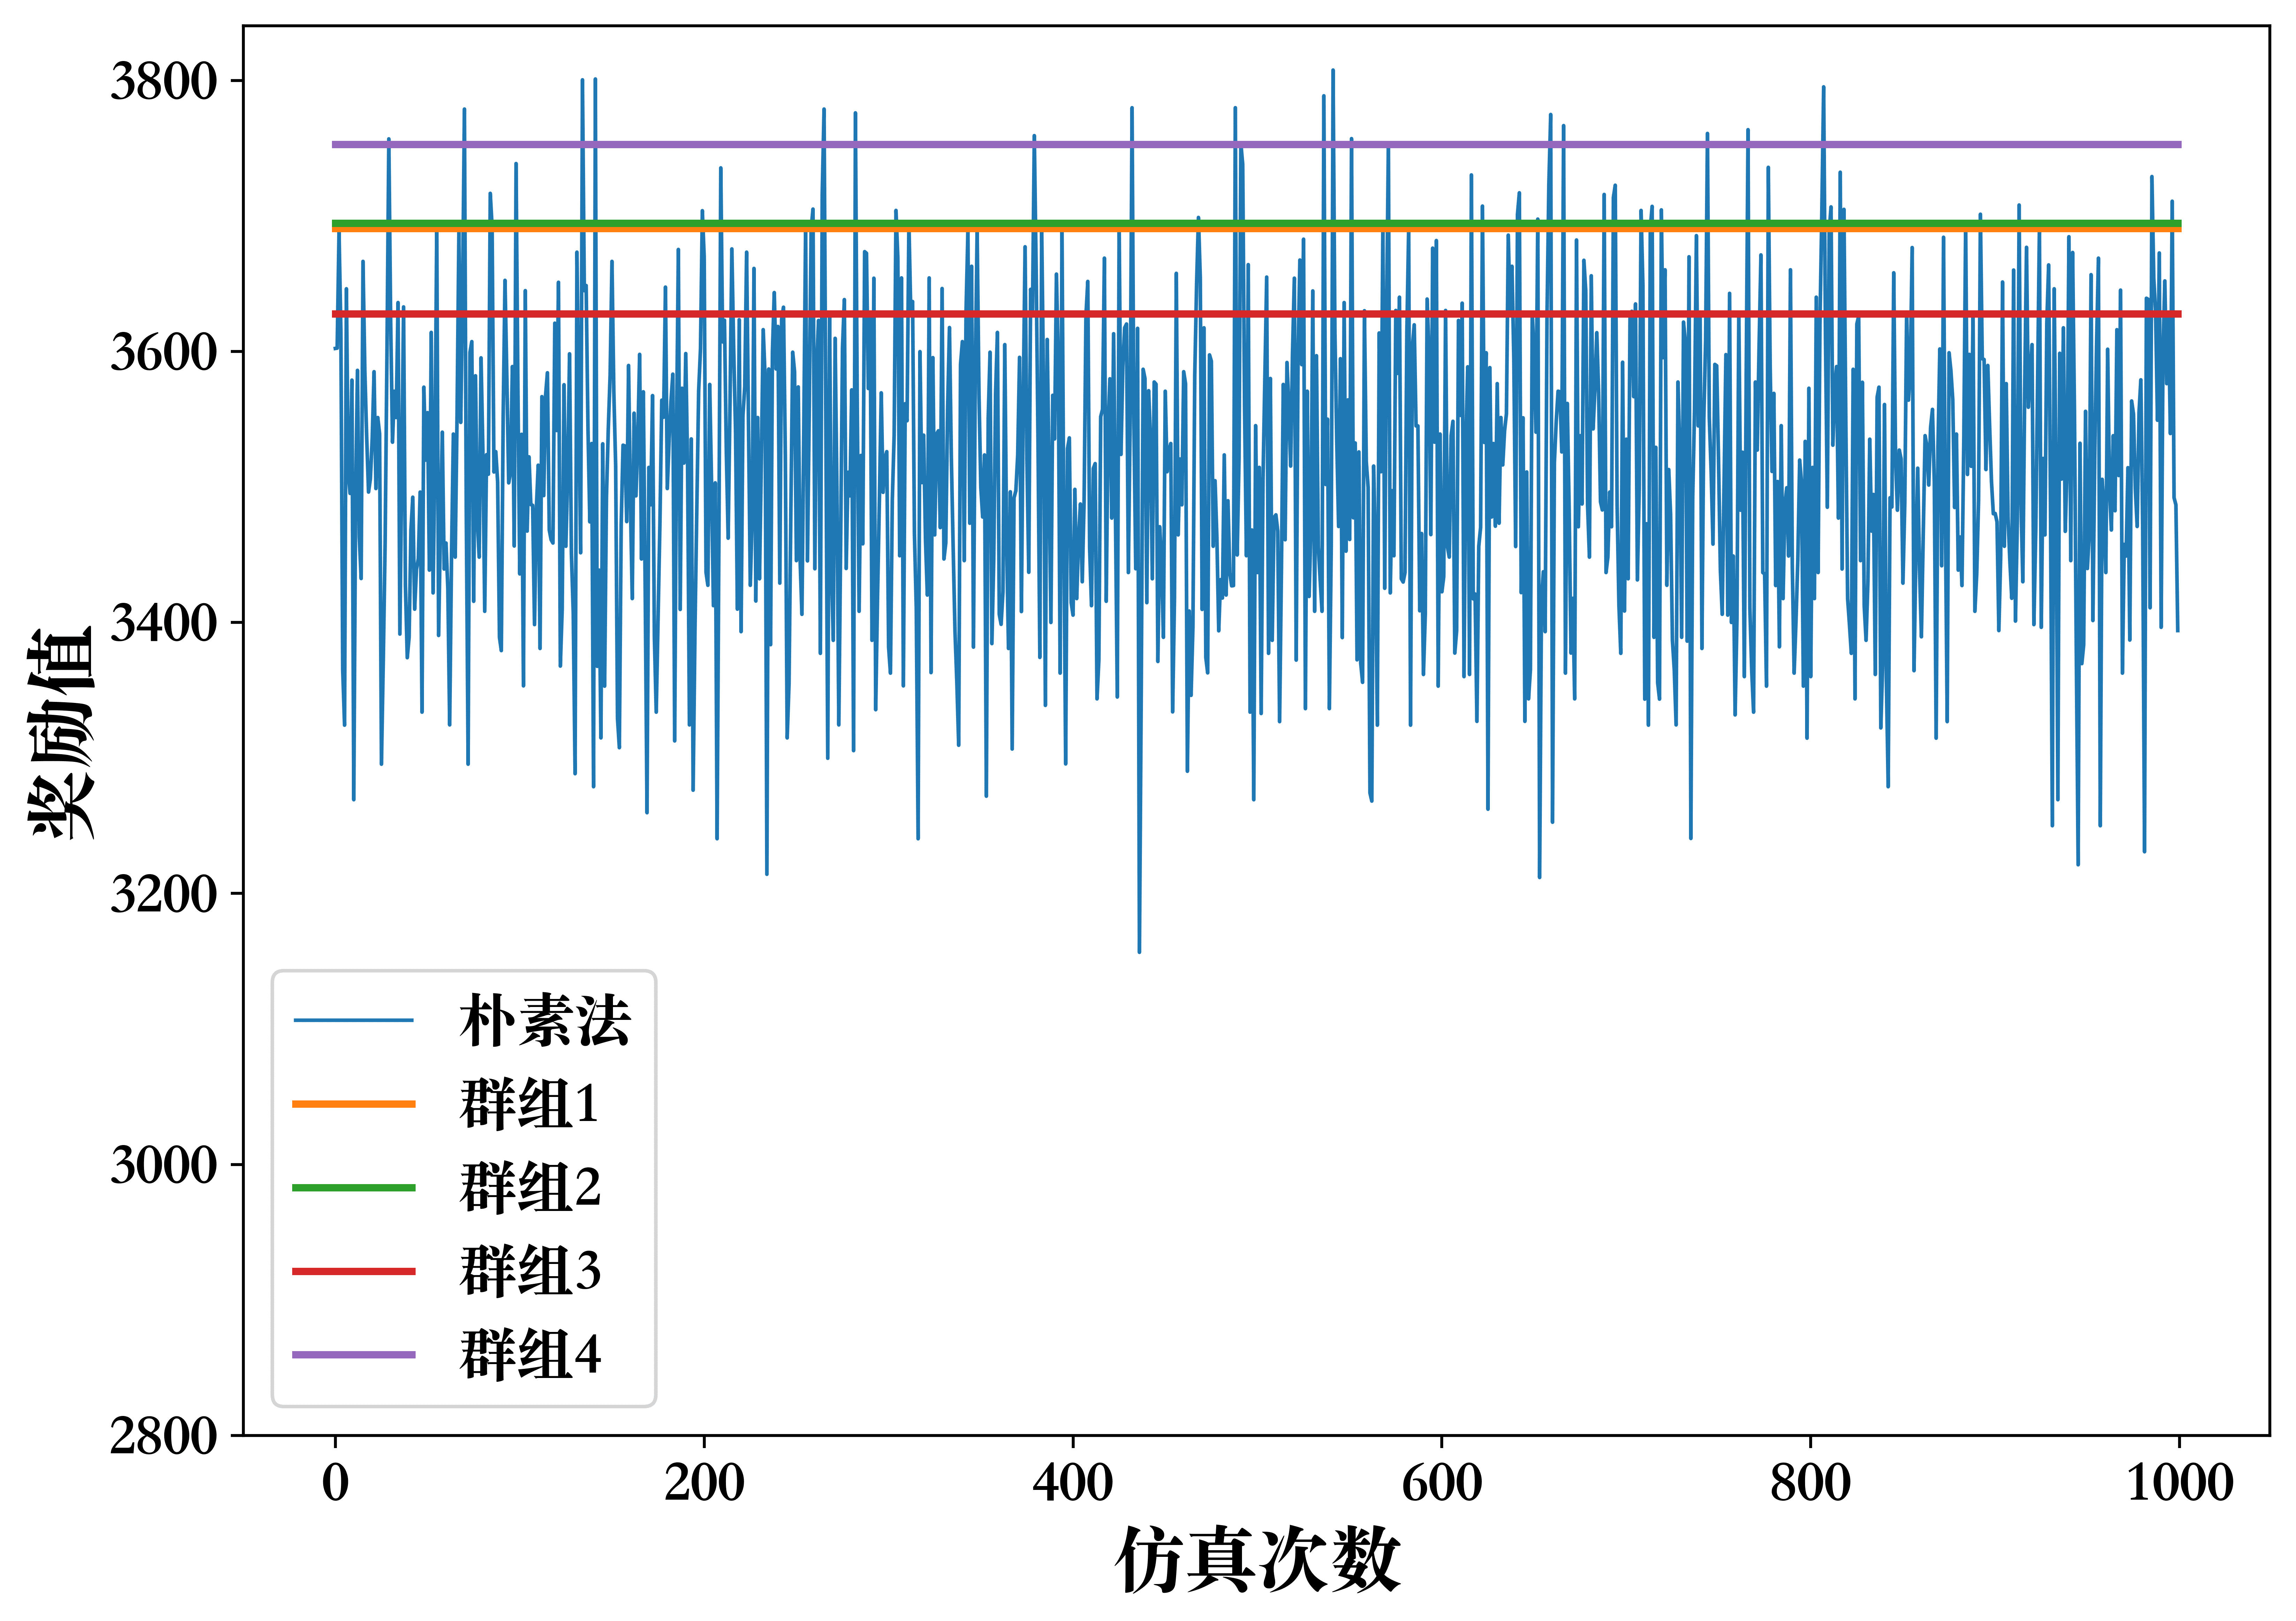
\includegraphics[width=.45\textwidth]{figures/content/agents/agent6.png}}
  \\
  \subfloat{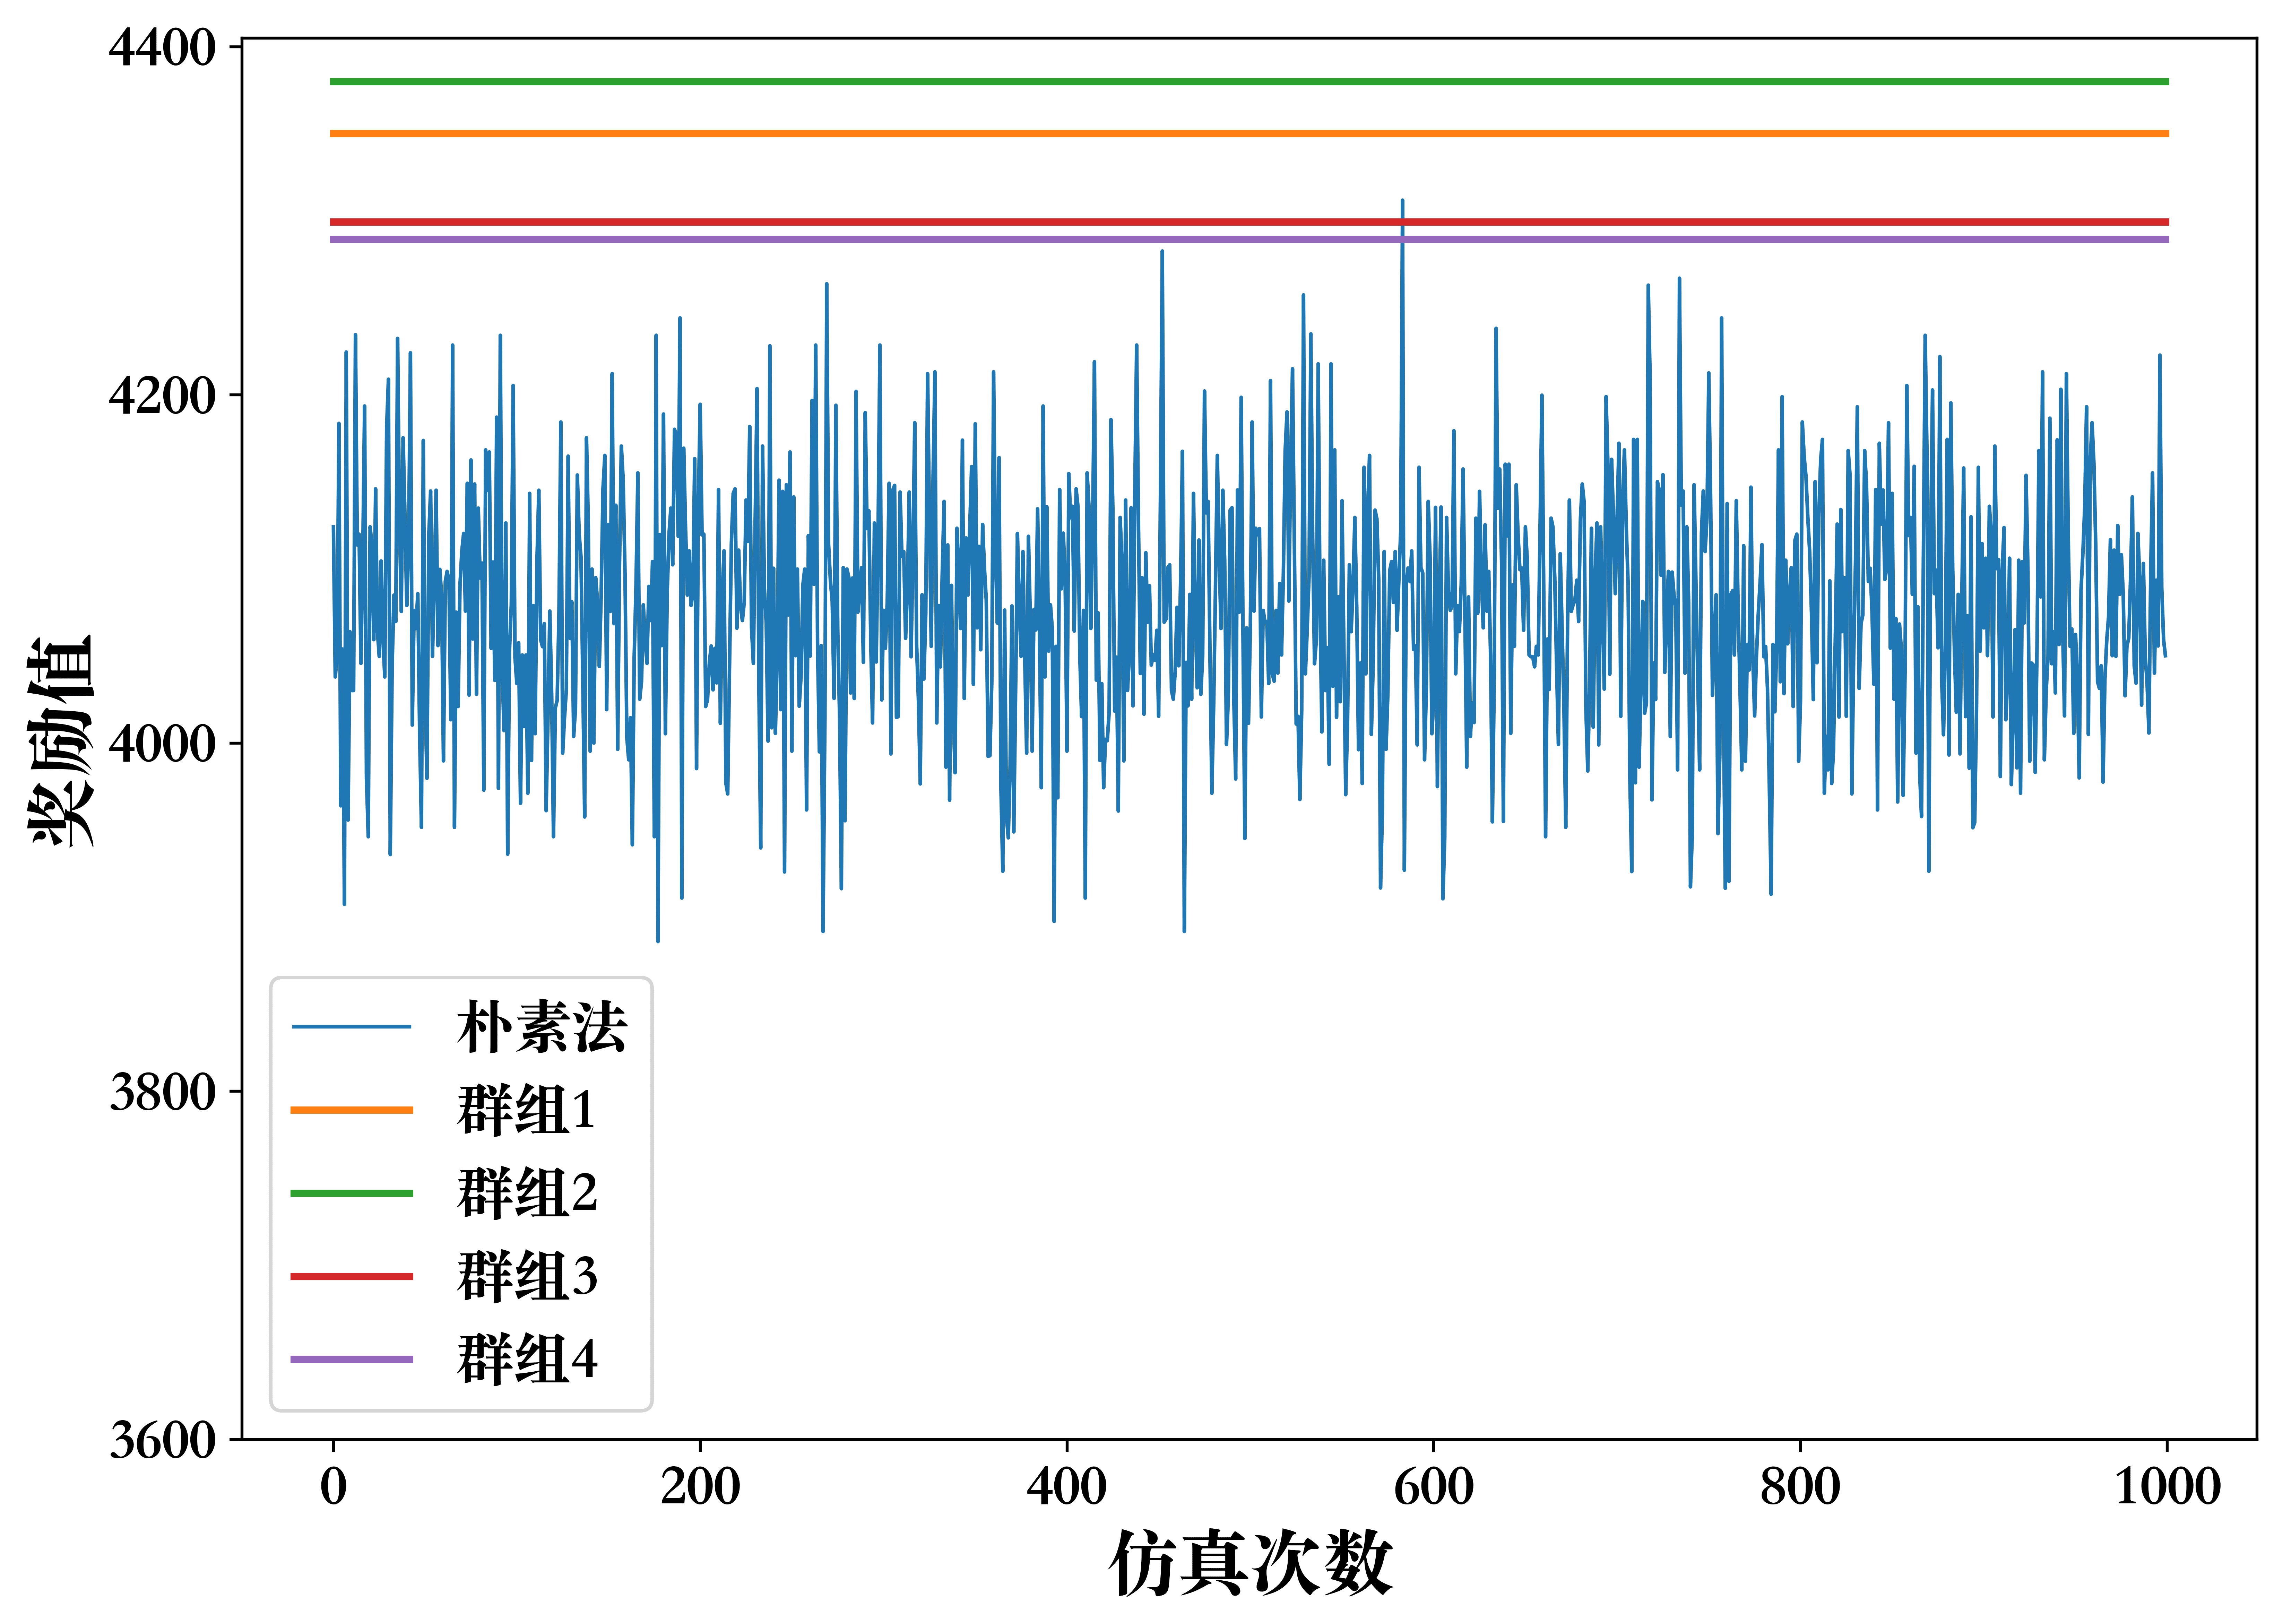
\includegraphics[width=.45\textwidth]{figures/content/agents/agent7.png}}
  \quad\quad
  \subfloat{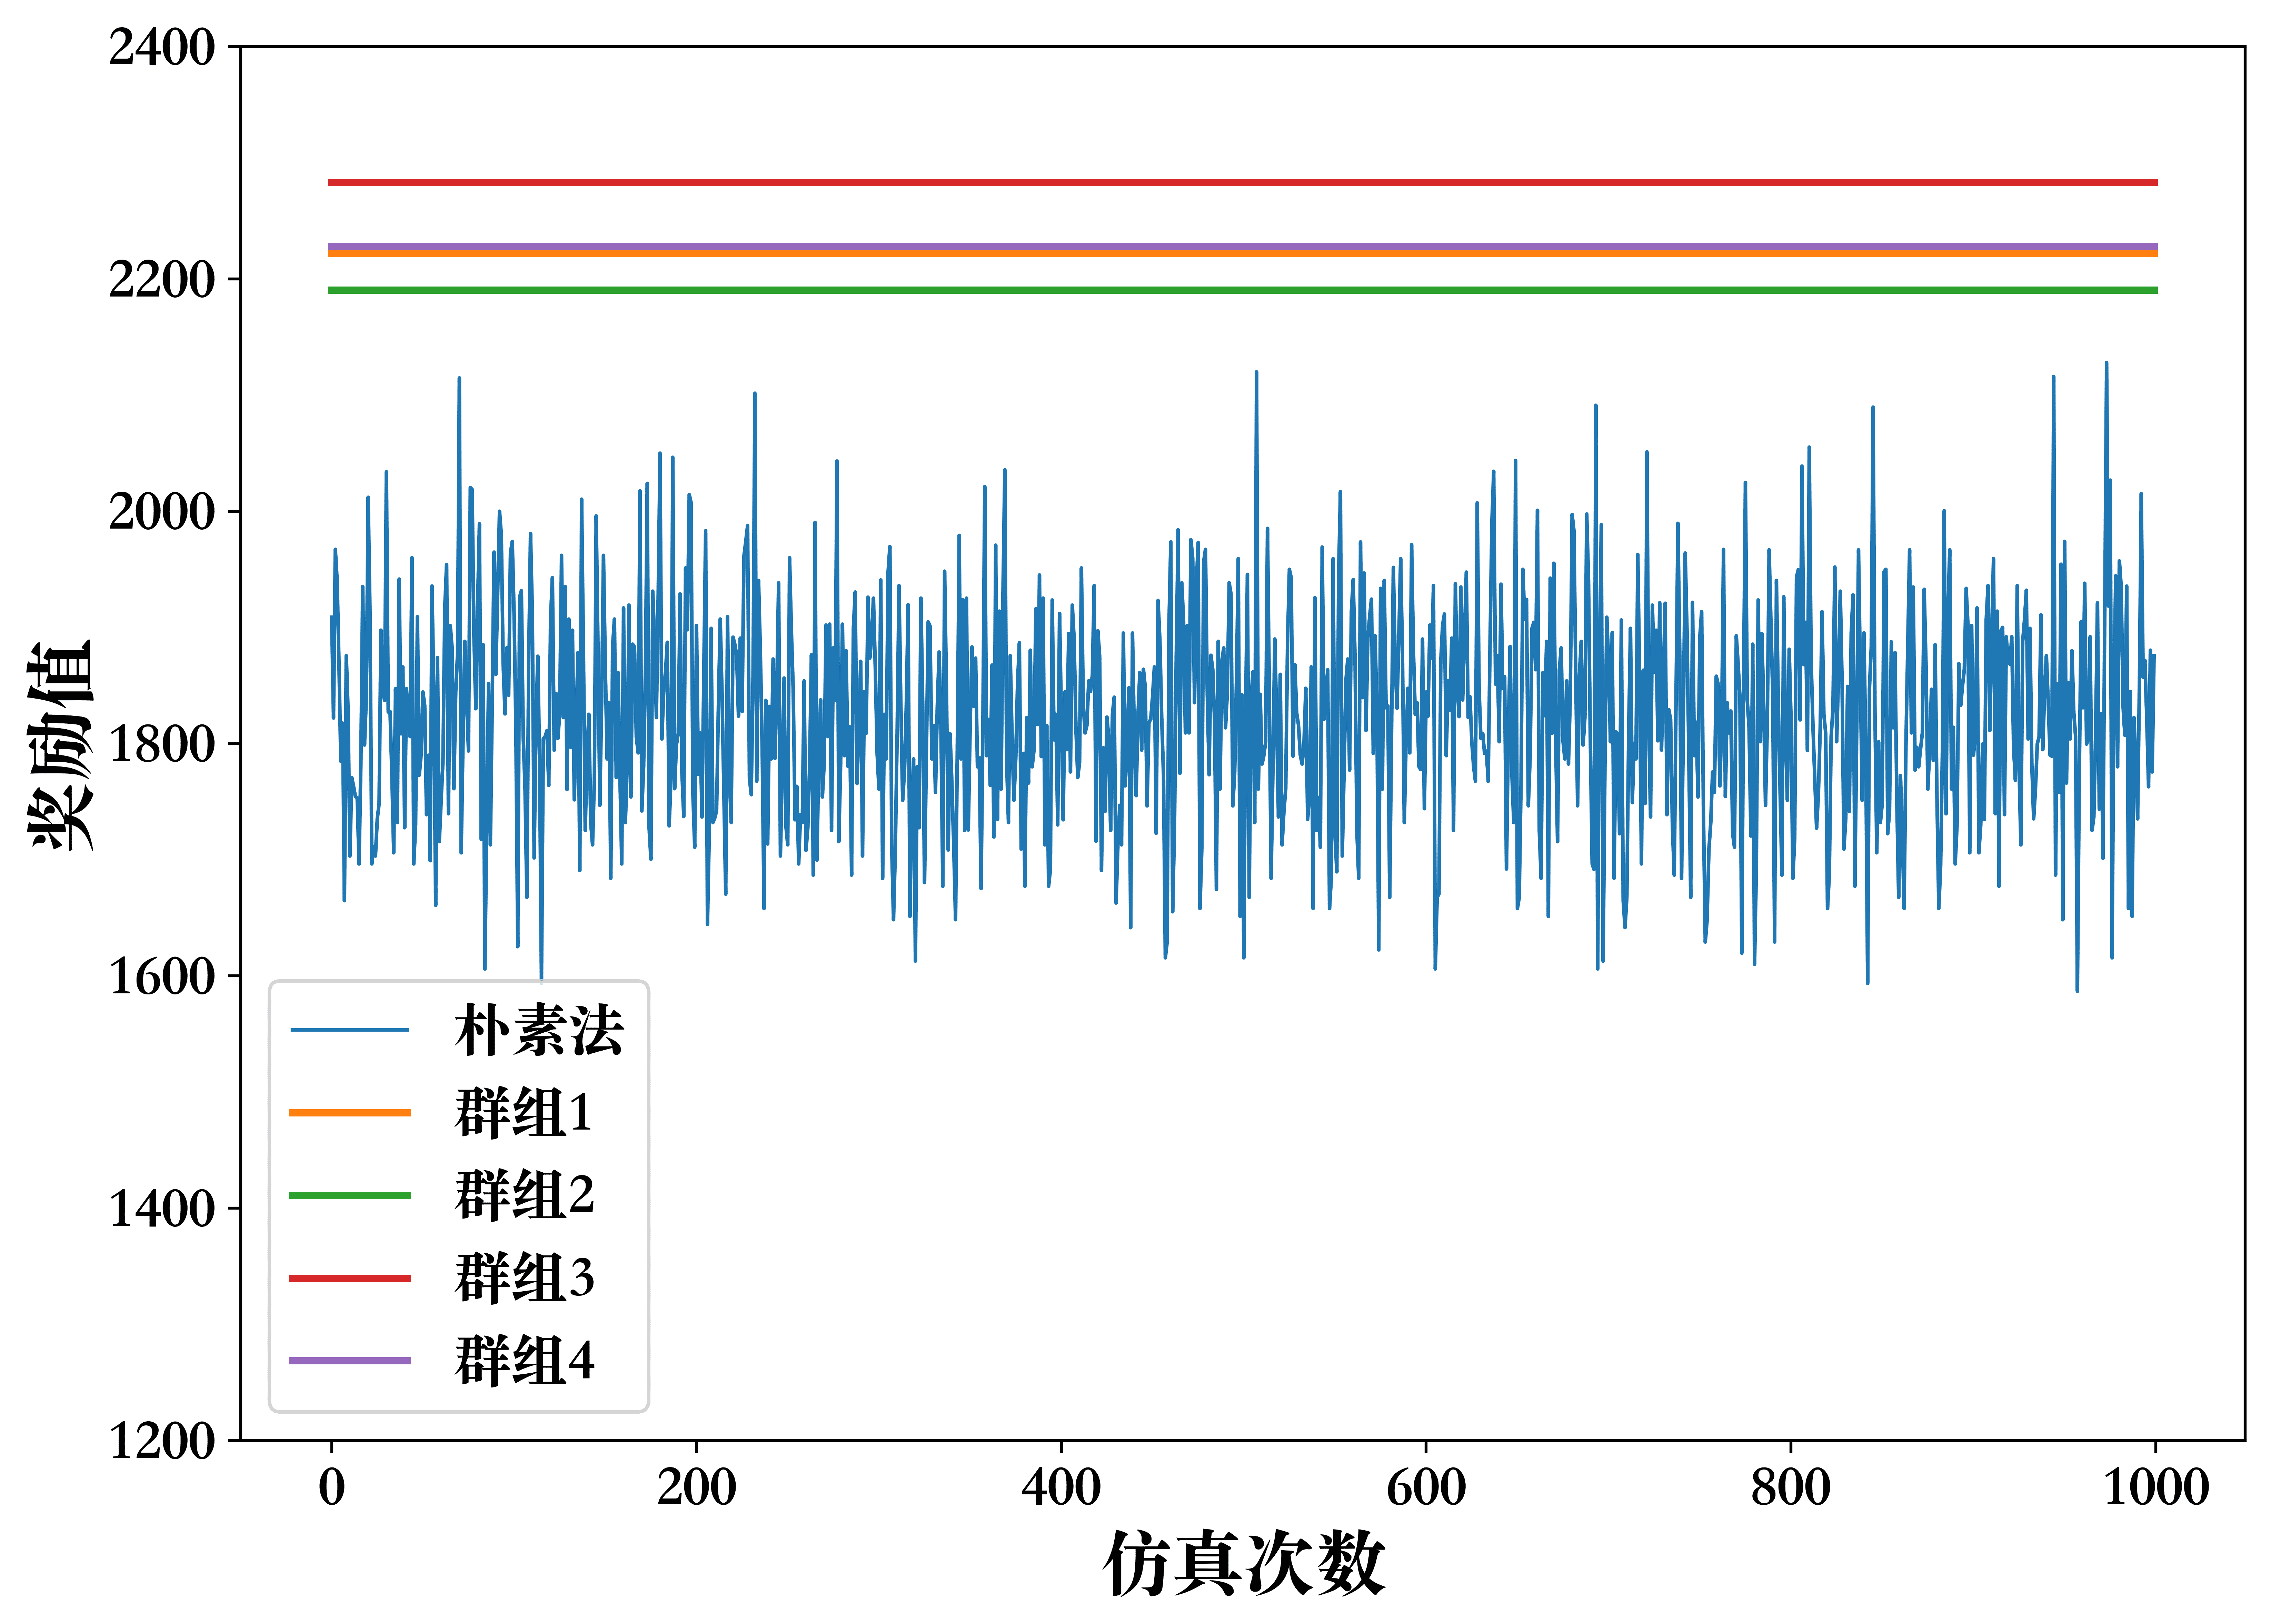
\includegraphics[width=.45\textwidth]{figures/content/agents/agent8.png}}
  \caption{不同智能体数量训练下的八个测试个体测试结果}
  \label{agents}
\end{figure}

\begin{table}[htbp]
\centering
\caption{不同智能体数量训练下所提出方法的性能变化}
\label{cluster_size}
\renewcommand{\arraystretch}{1.2} % 使表格行间距加大1.2倍
\setlength{\tabcolsep}{6mm} % 设置列间距为6mm
\small % 调整字体大小为small

\begin{tabular}{lccccc}
\toprule
代表点数量     & 1  & 4  & 10 & 20  & 40                \\ \midrule
训练时间 (小时)  & 5        & 22        & 68         & 140        & \textbackslash{}       \\
平均奖励值 & 2,684      & 3,203      & 3,351       & 3,394        & \textbackslash{}   \\
超过95(共50次)的次数     & 16        & 41         & 45          & 46          & \textbackslash{}\\ \bottomrule
\end{tabular}
\end{table}

\begin{figure}
  \centering
  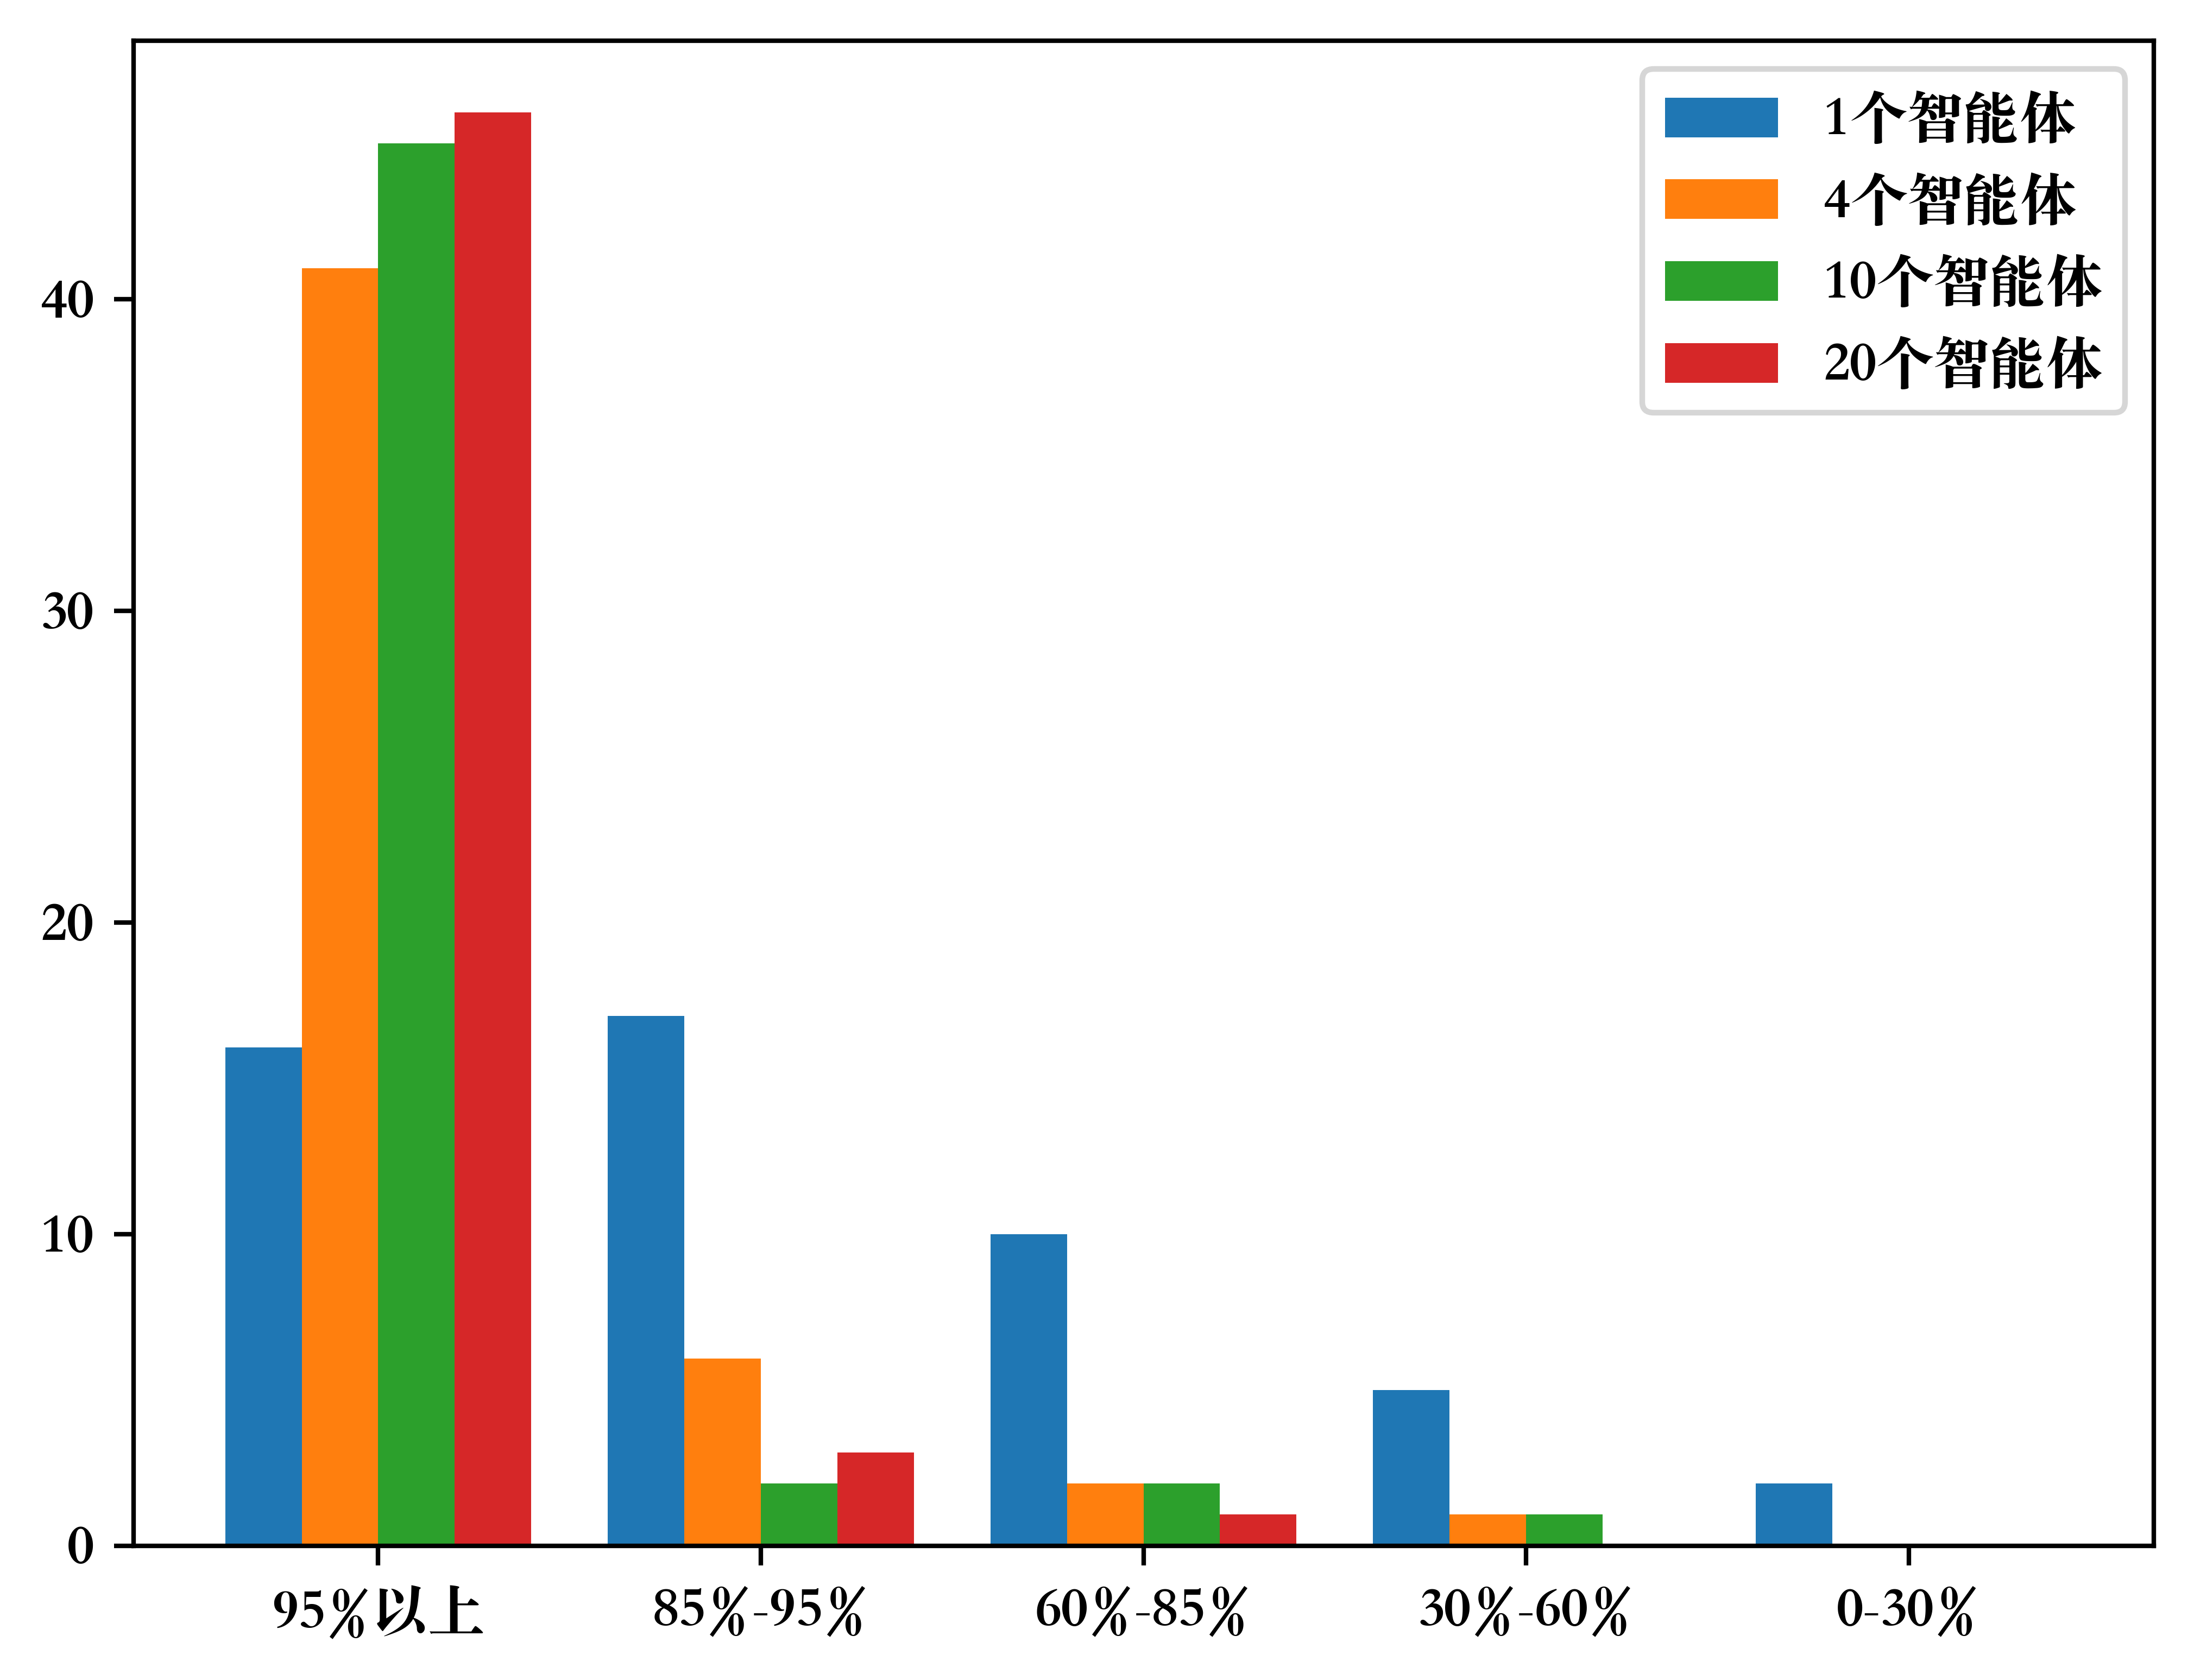
\includegraphics[width=.75\linewidth]{figures/content/number.png}
  \caption{不同智能体数量训练下与朴素法最大奖励值的比较}
  \label{agent_map}
\end{figure}


为了显示所提出方法的性能并不因每个类别中挑选训练个体的不同而发生显著变化,使用不同的训练个体集合进行另一组实验,挑选在每个类别中挑选四个智能体进行训练,其余的实验设置保持不变。表\ref{cluster_agents}列出了这样四个实验的结果。由于不同的训练个体集合不会改变计算时间(对于四个代表,计算时间为22小时),因此不再报告这个度量。从结果中可以看出,所提出方法的性能是稳定的,不会因为用于训练的代表个体不同而表现出显著的变化。类似于图\ref{agents},图\ref{size}显示了当使用不同的训练个体集合时,八个选定测试个体结果的比较,表明所提出的方法对代表个体的选择具有鲁棒性。这些结果表明,所提出的方法是有效的,不会受到训练代表个体集合的影响。从这些敏感性分析中可以得出结论,所提出的方法在实际应用中具有很强的可操作性和鲁棒性。通过将模型应用于新的时间依赖 OD 数据集并比较与传统模型和朴素法的性能,证明了该方法在解决模式选择与出发时间问题方面的有效性。

\begin{figure}[htbp]
  \subfloat{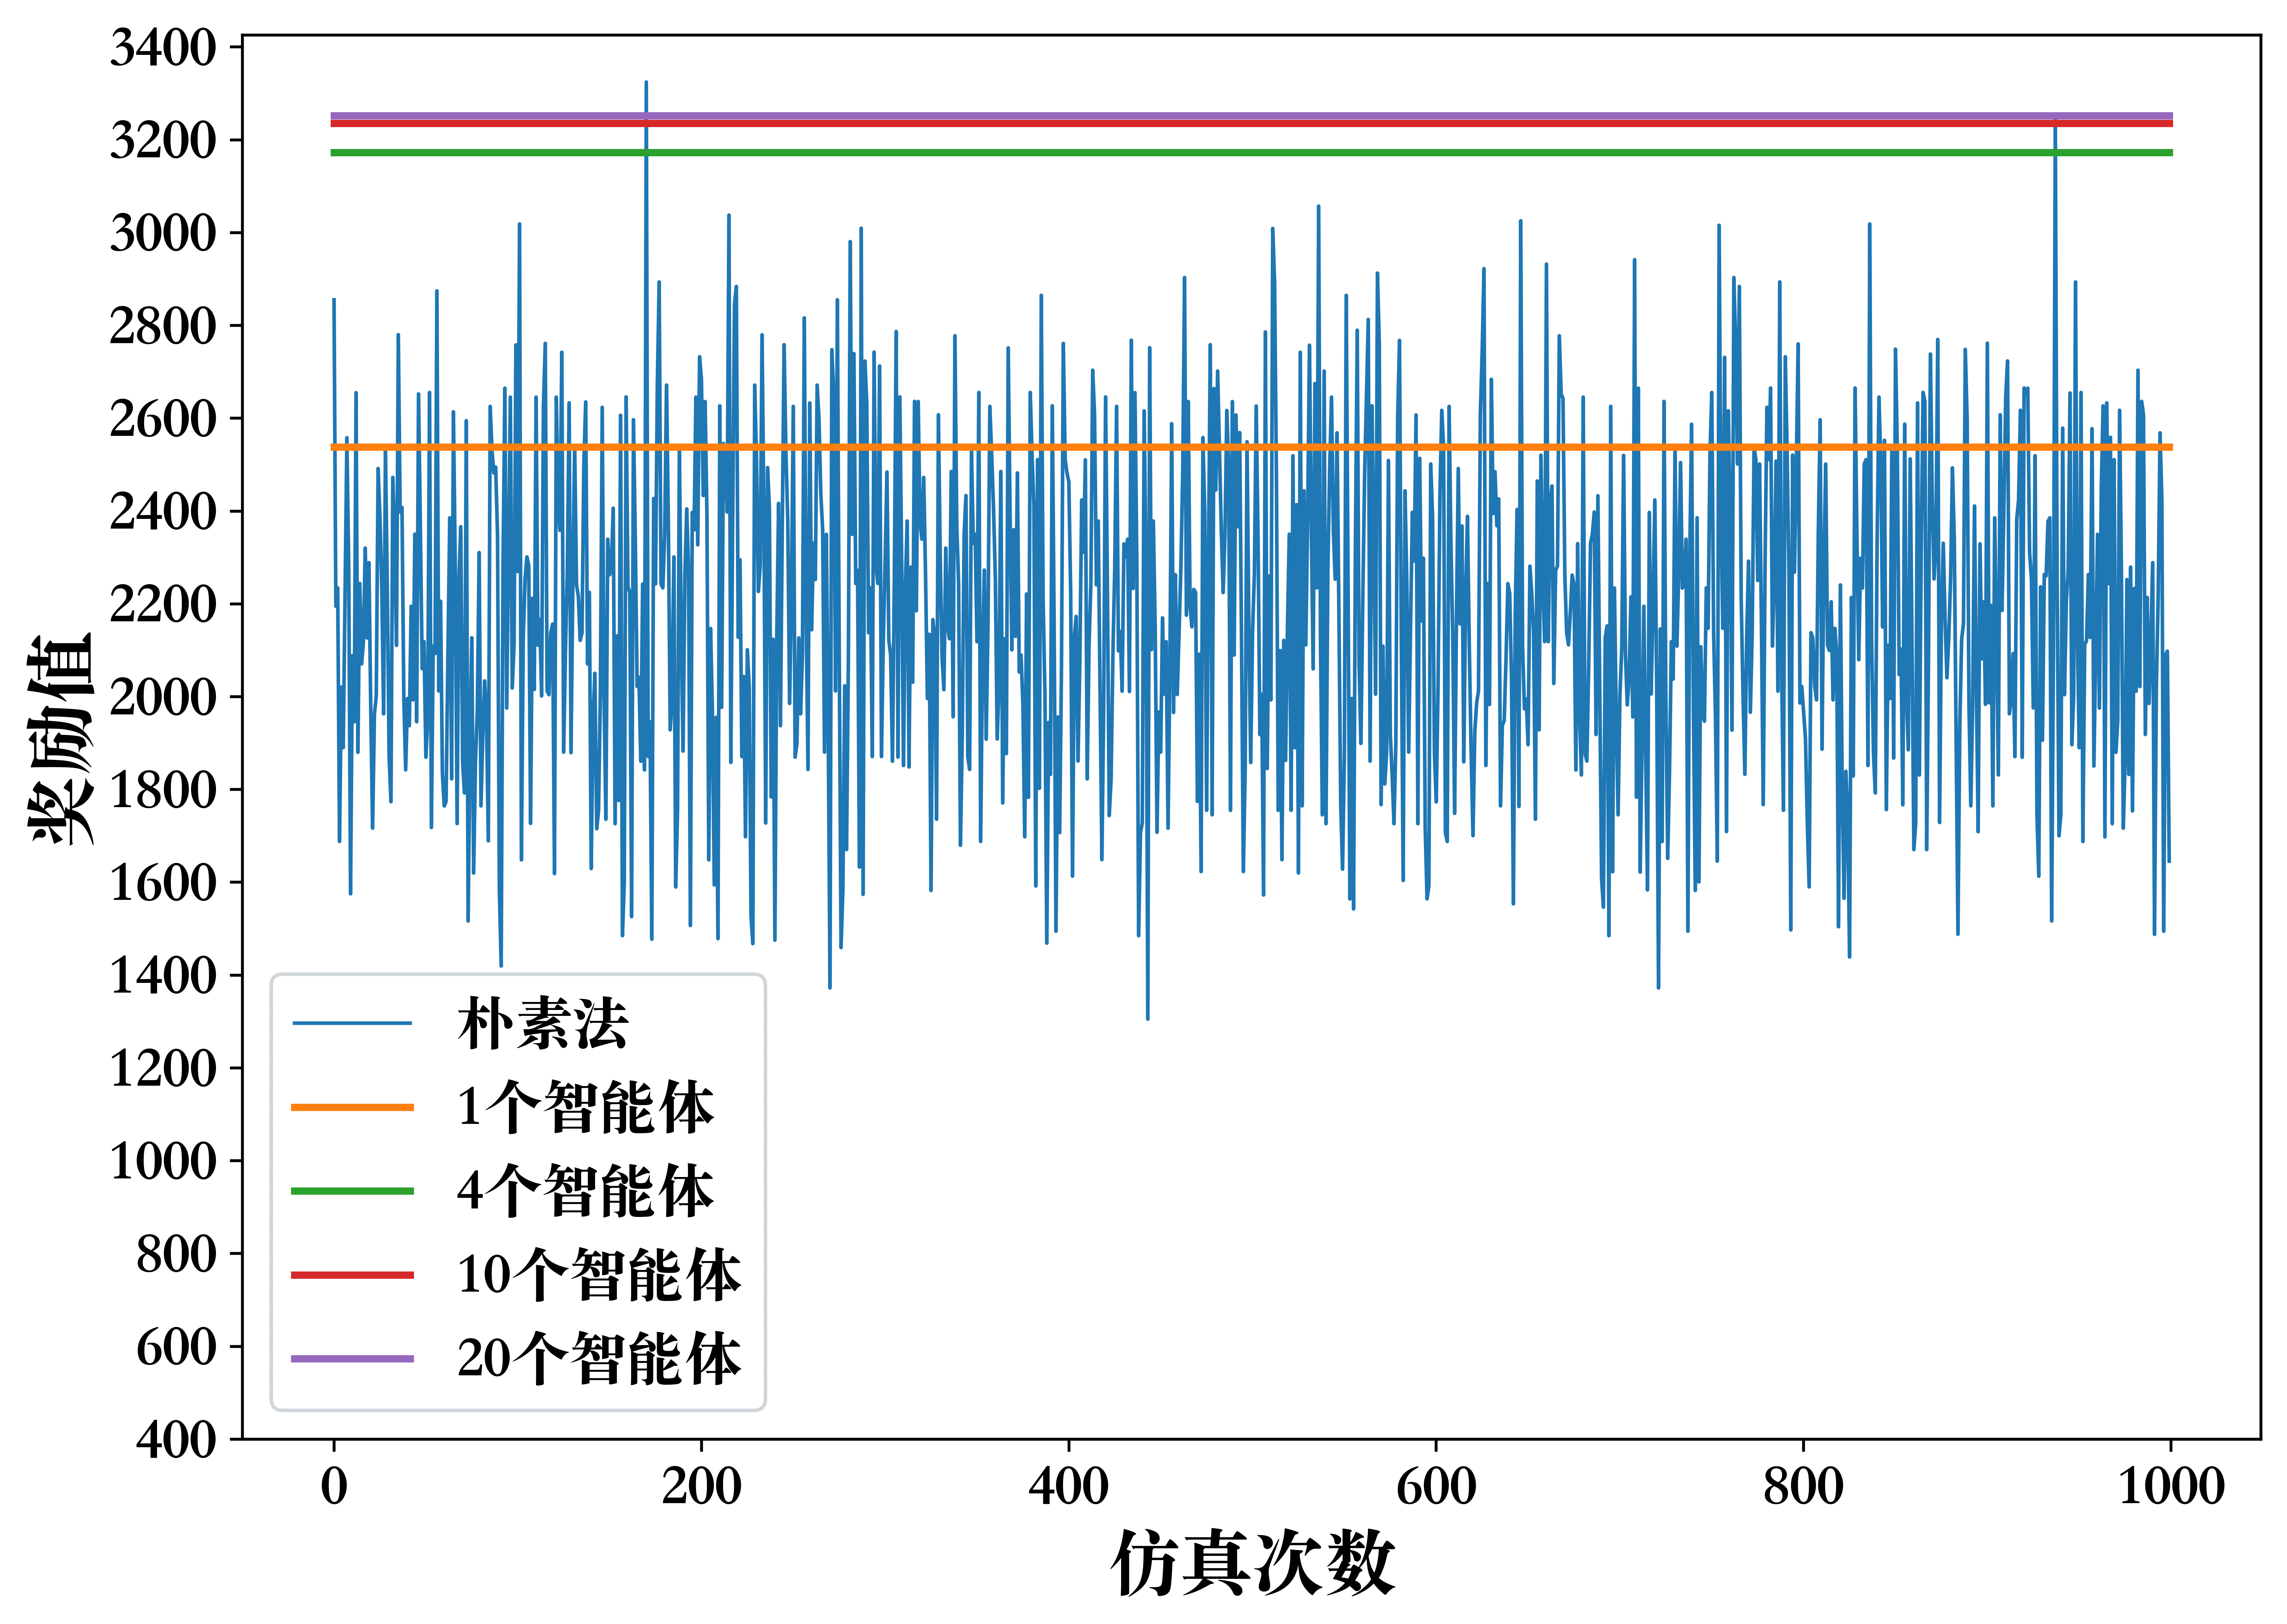
\includegraphics[width=.45\textwidth]{figures/content/size/size1.png}}
  \quad\quad
  \subfloat{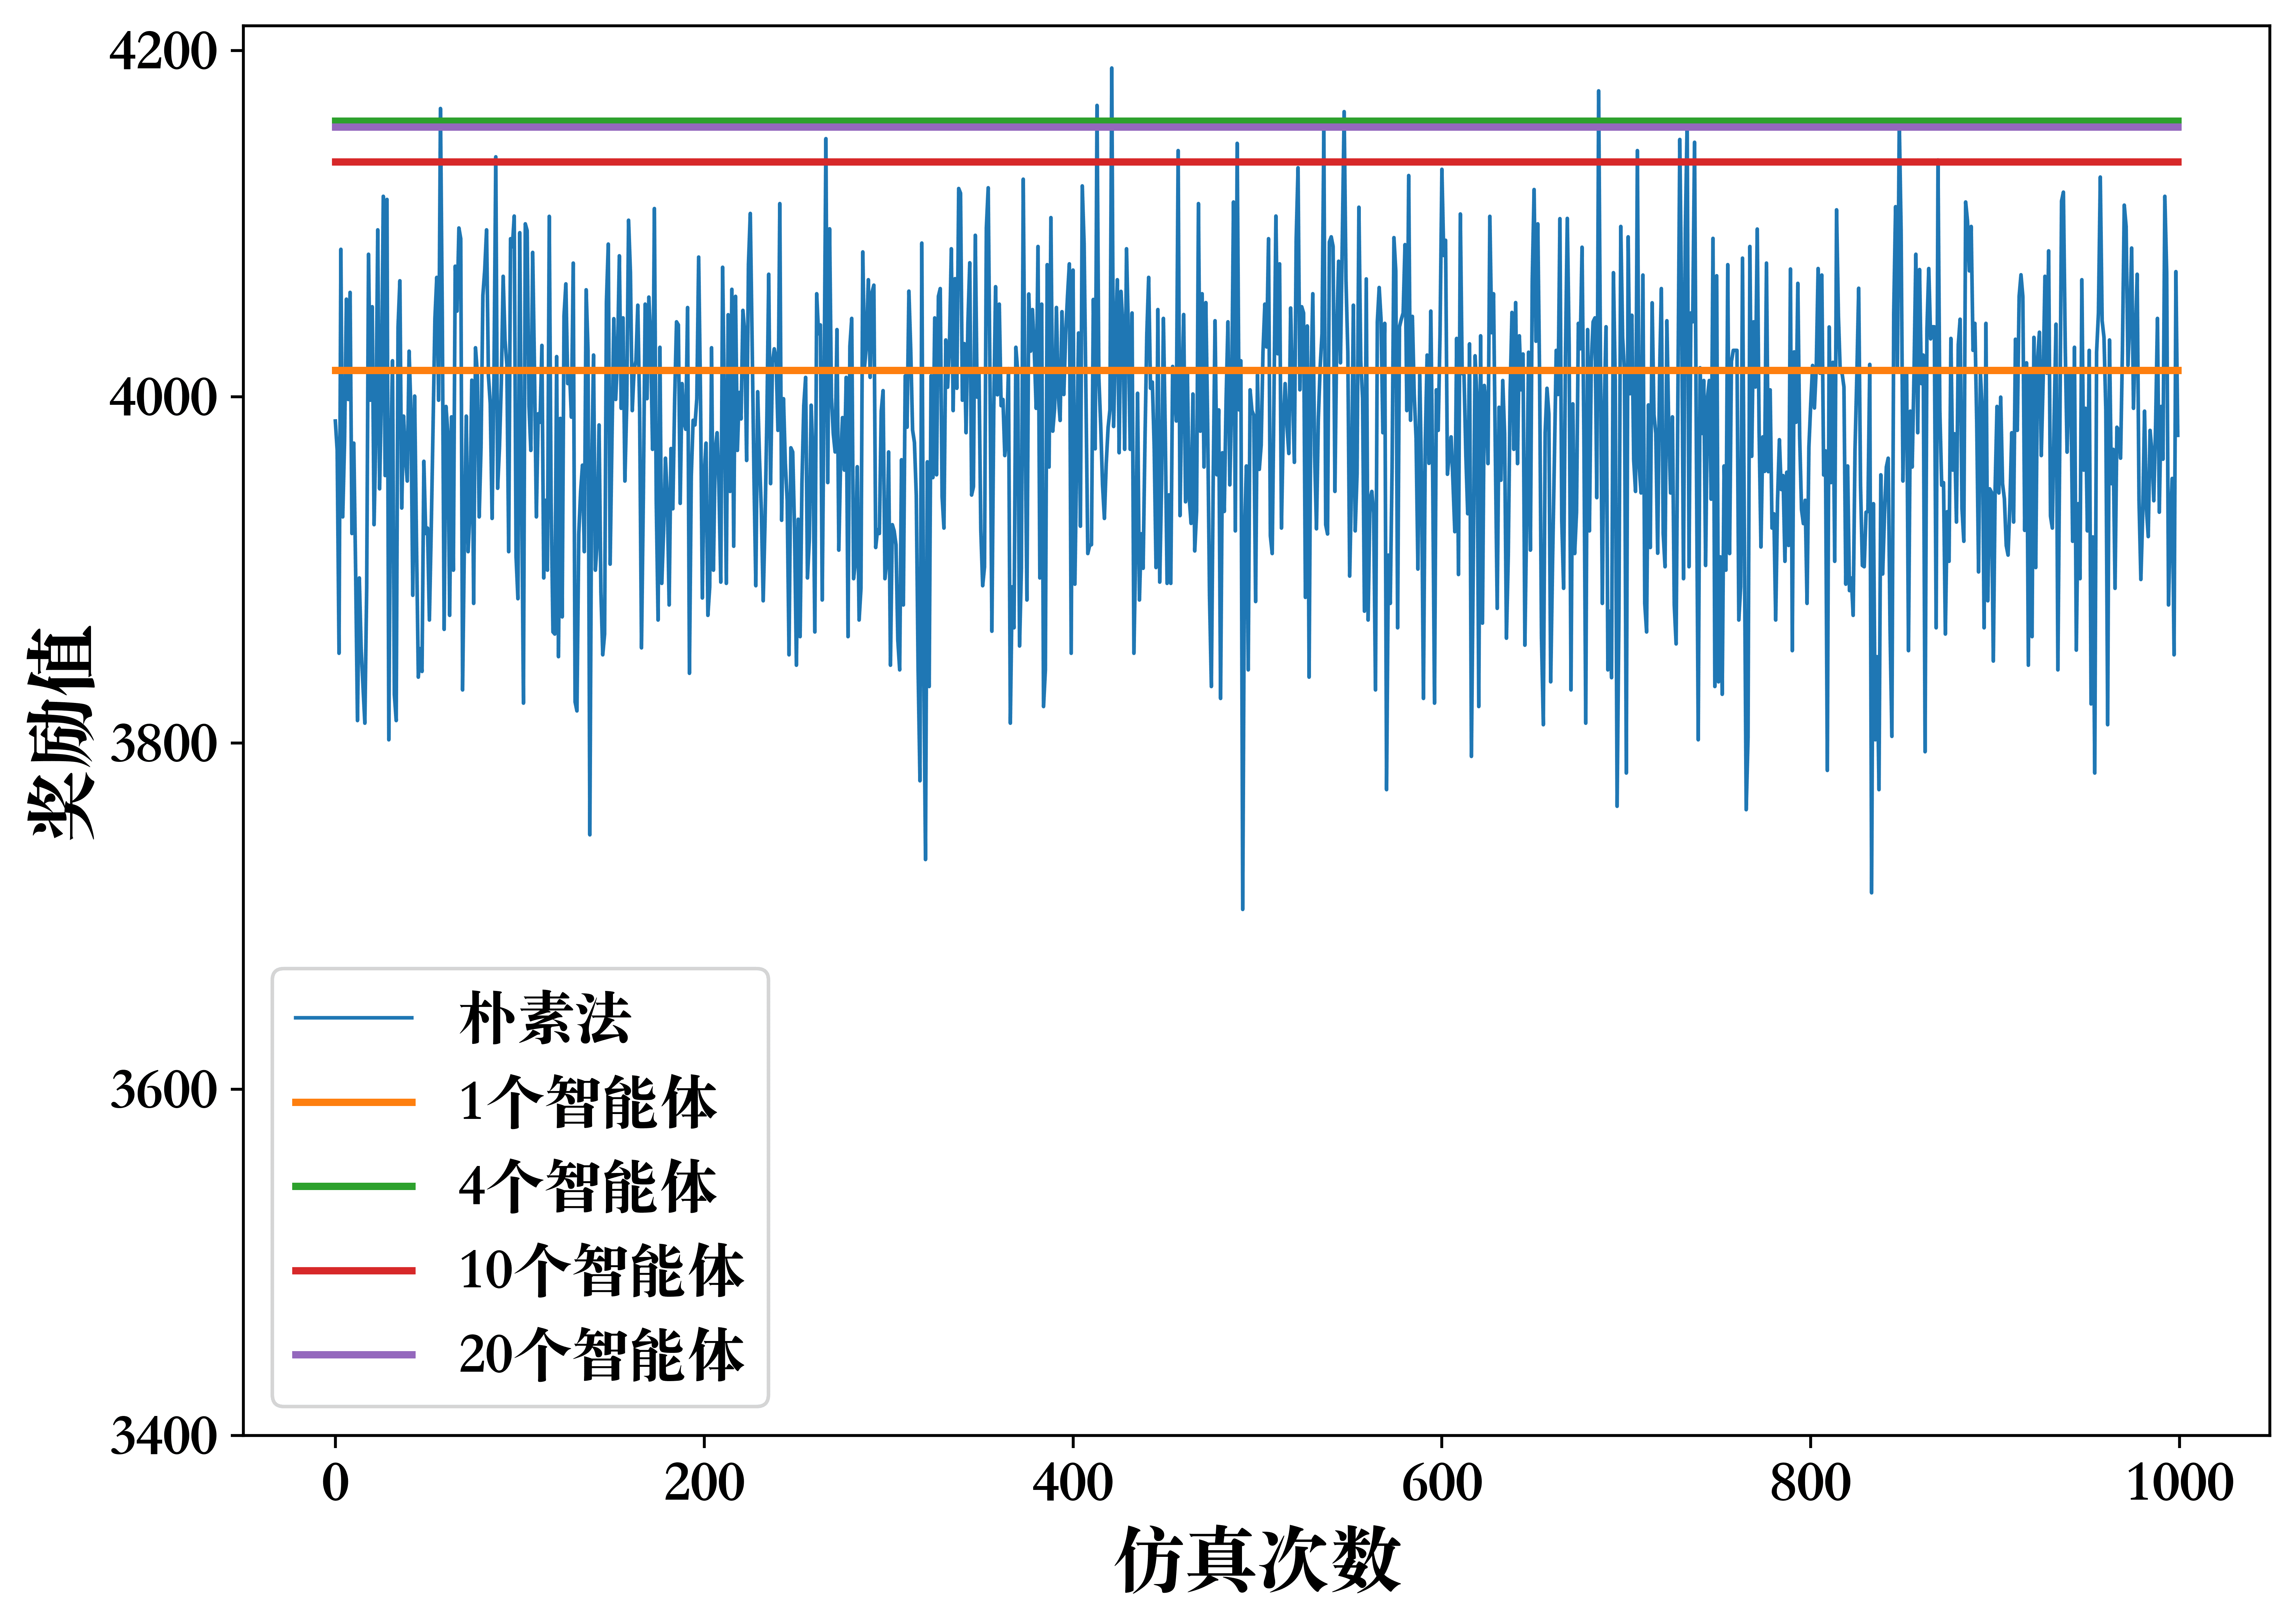
\includegraphics[width=.45\textwidth]{figures/content/size/size2.png}}
  \\
  \subfloat{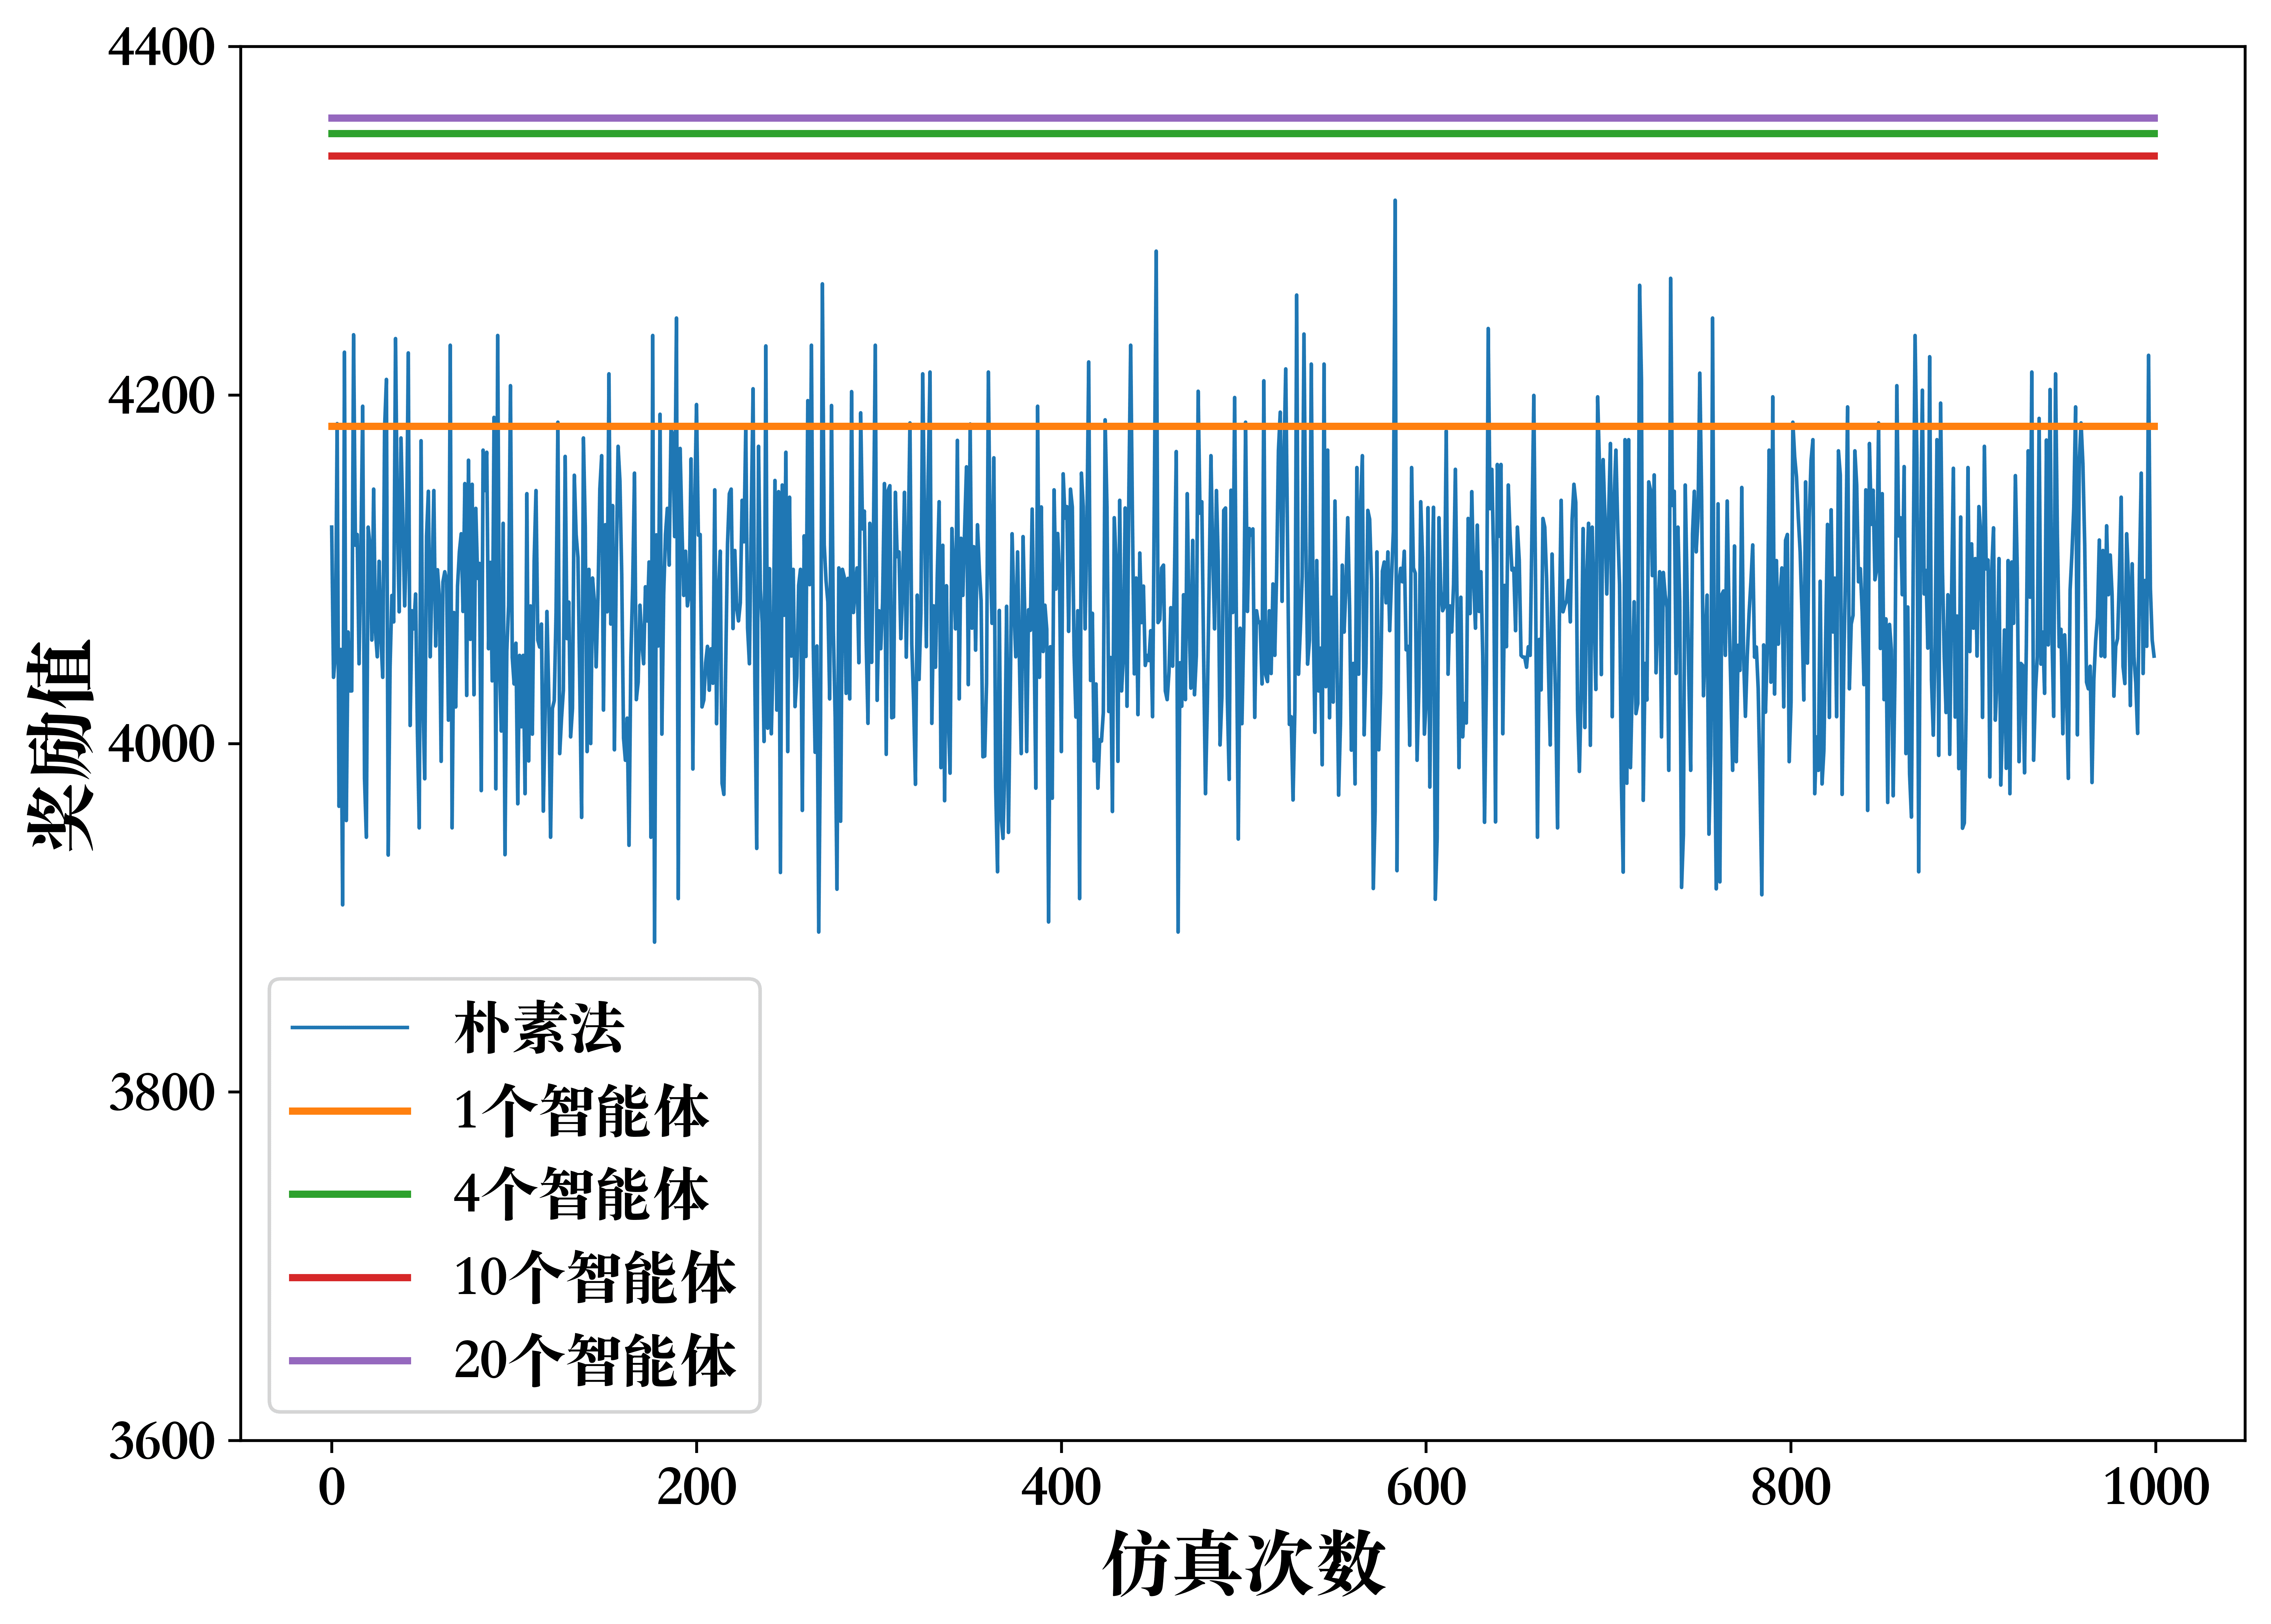
\includegraphics[width=.45\textwidth]{figures/content/size/size3.png}}
  \quad\quad
  \subfloat{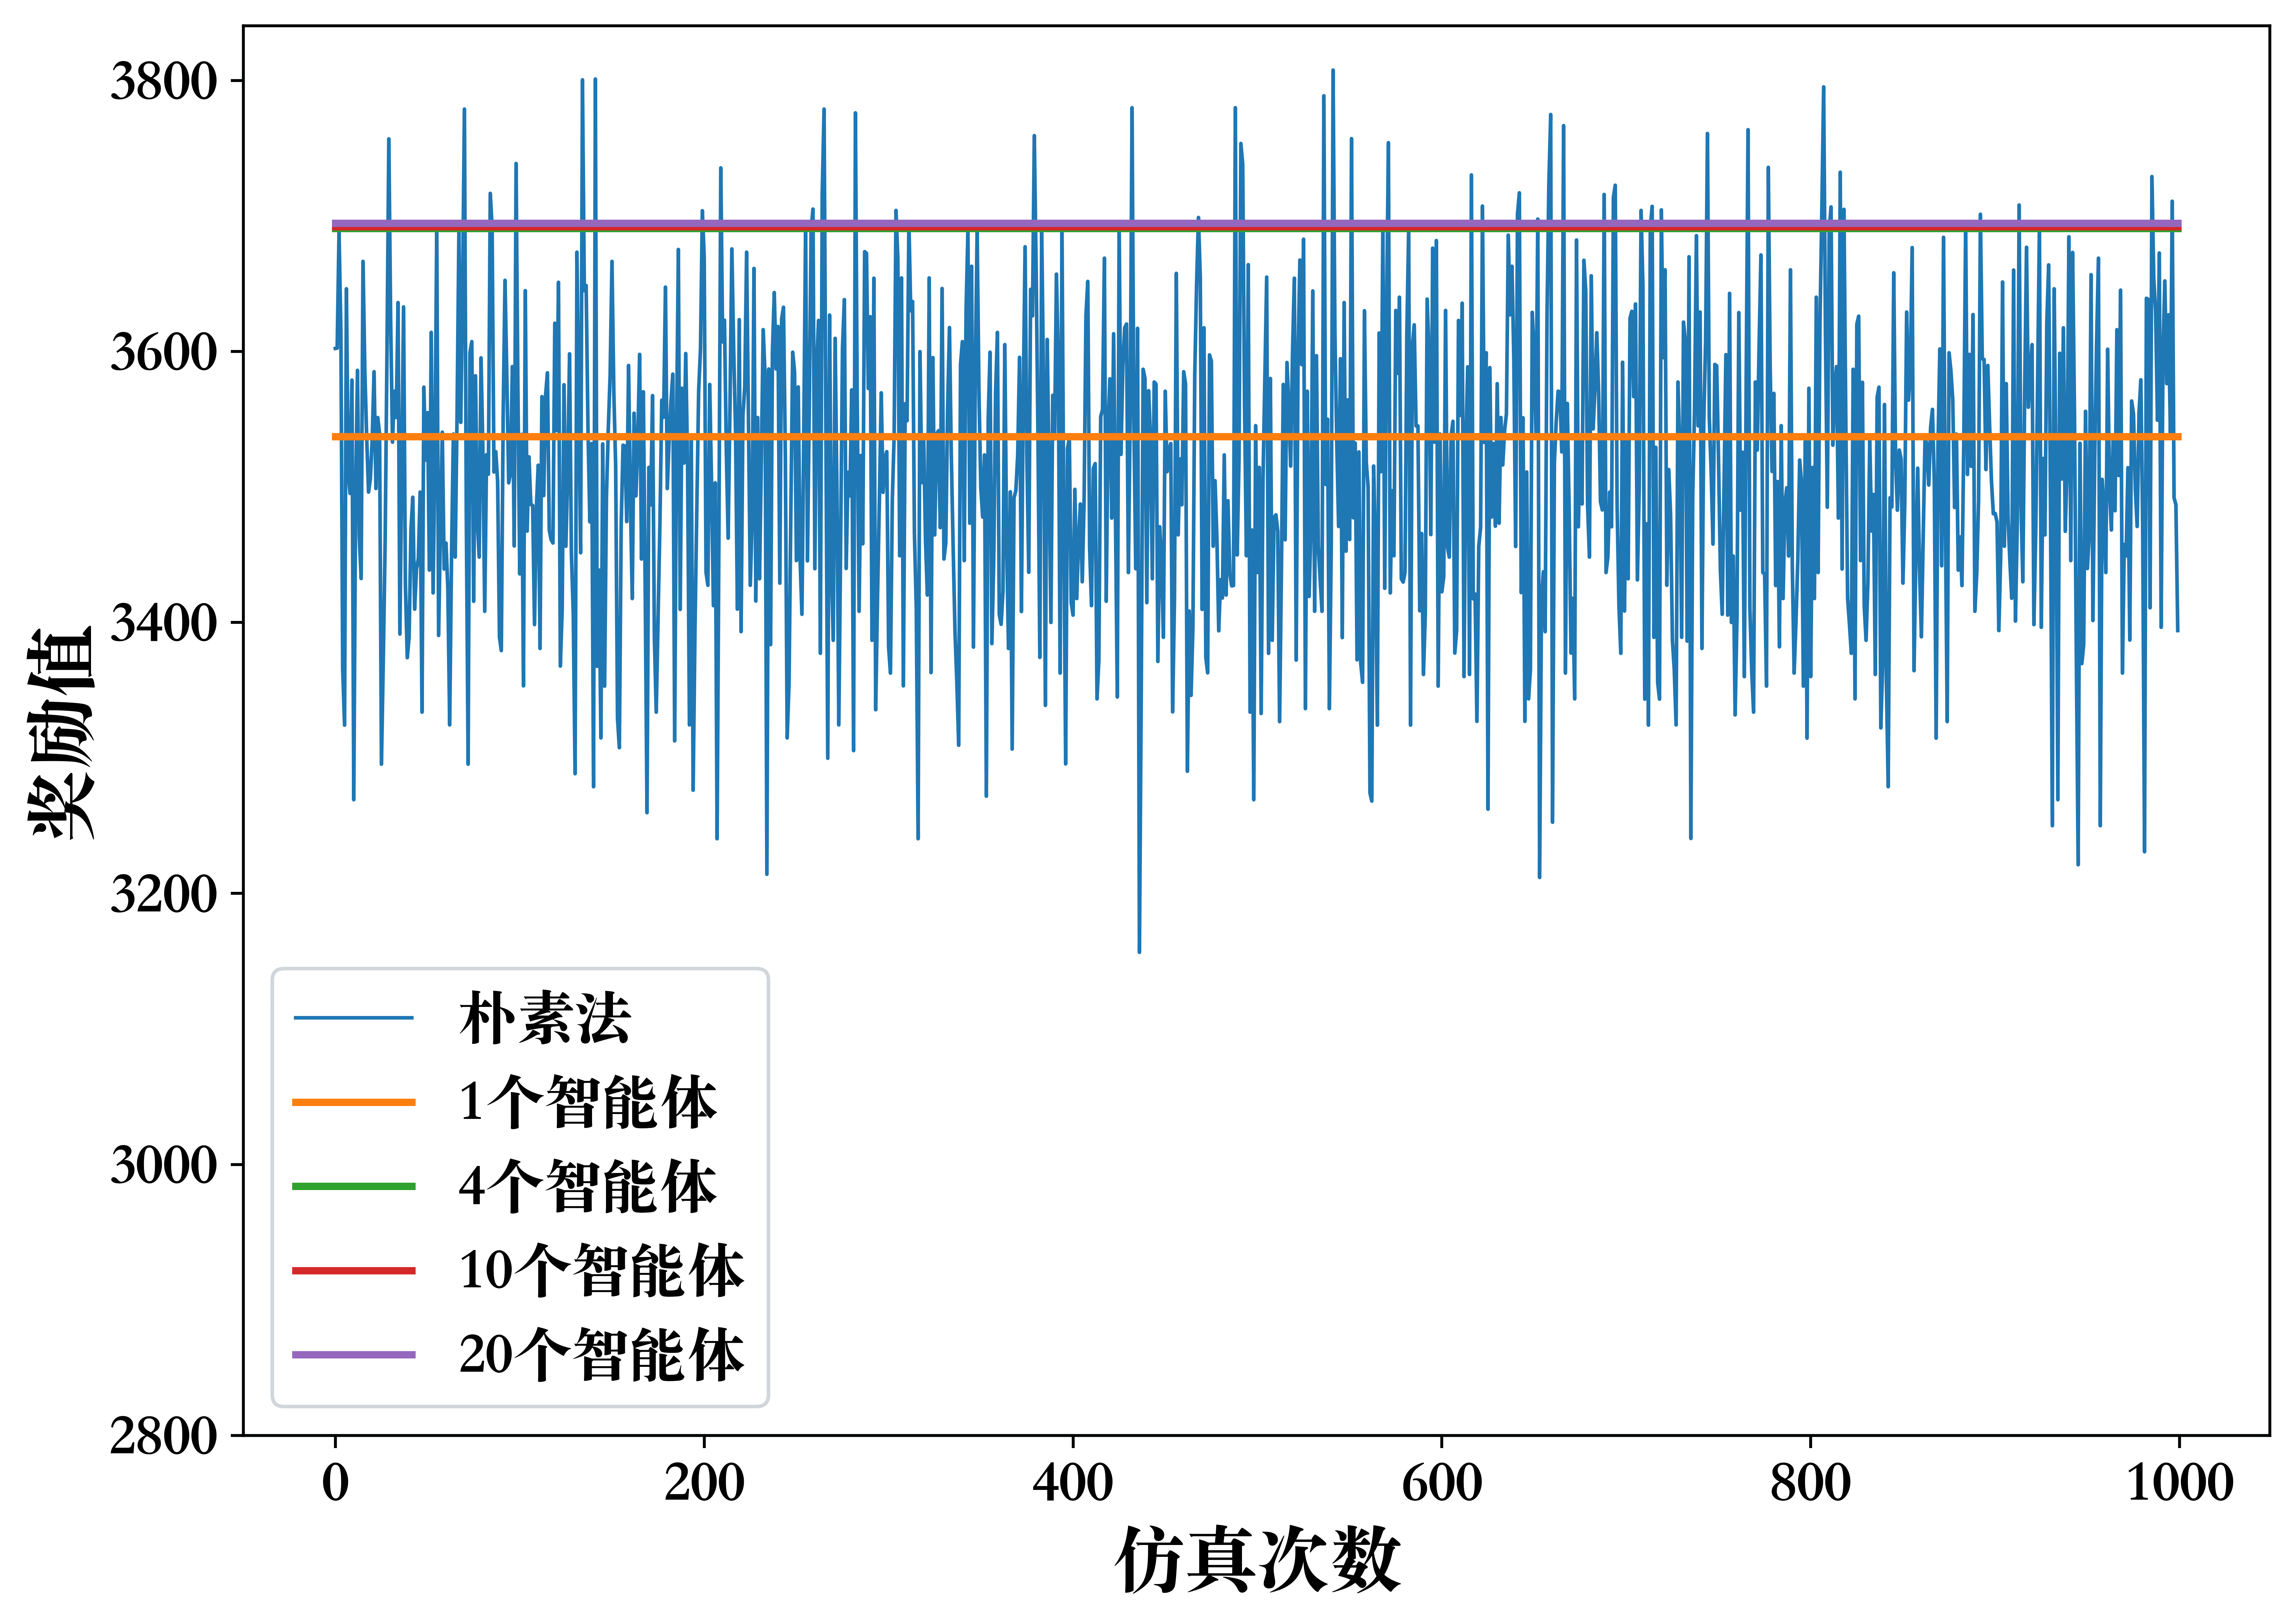
\includegraphics[width=.45\textwidth]{figures/content/size/size4.png}}
  \\
  \subfloat{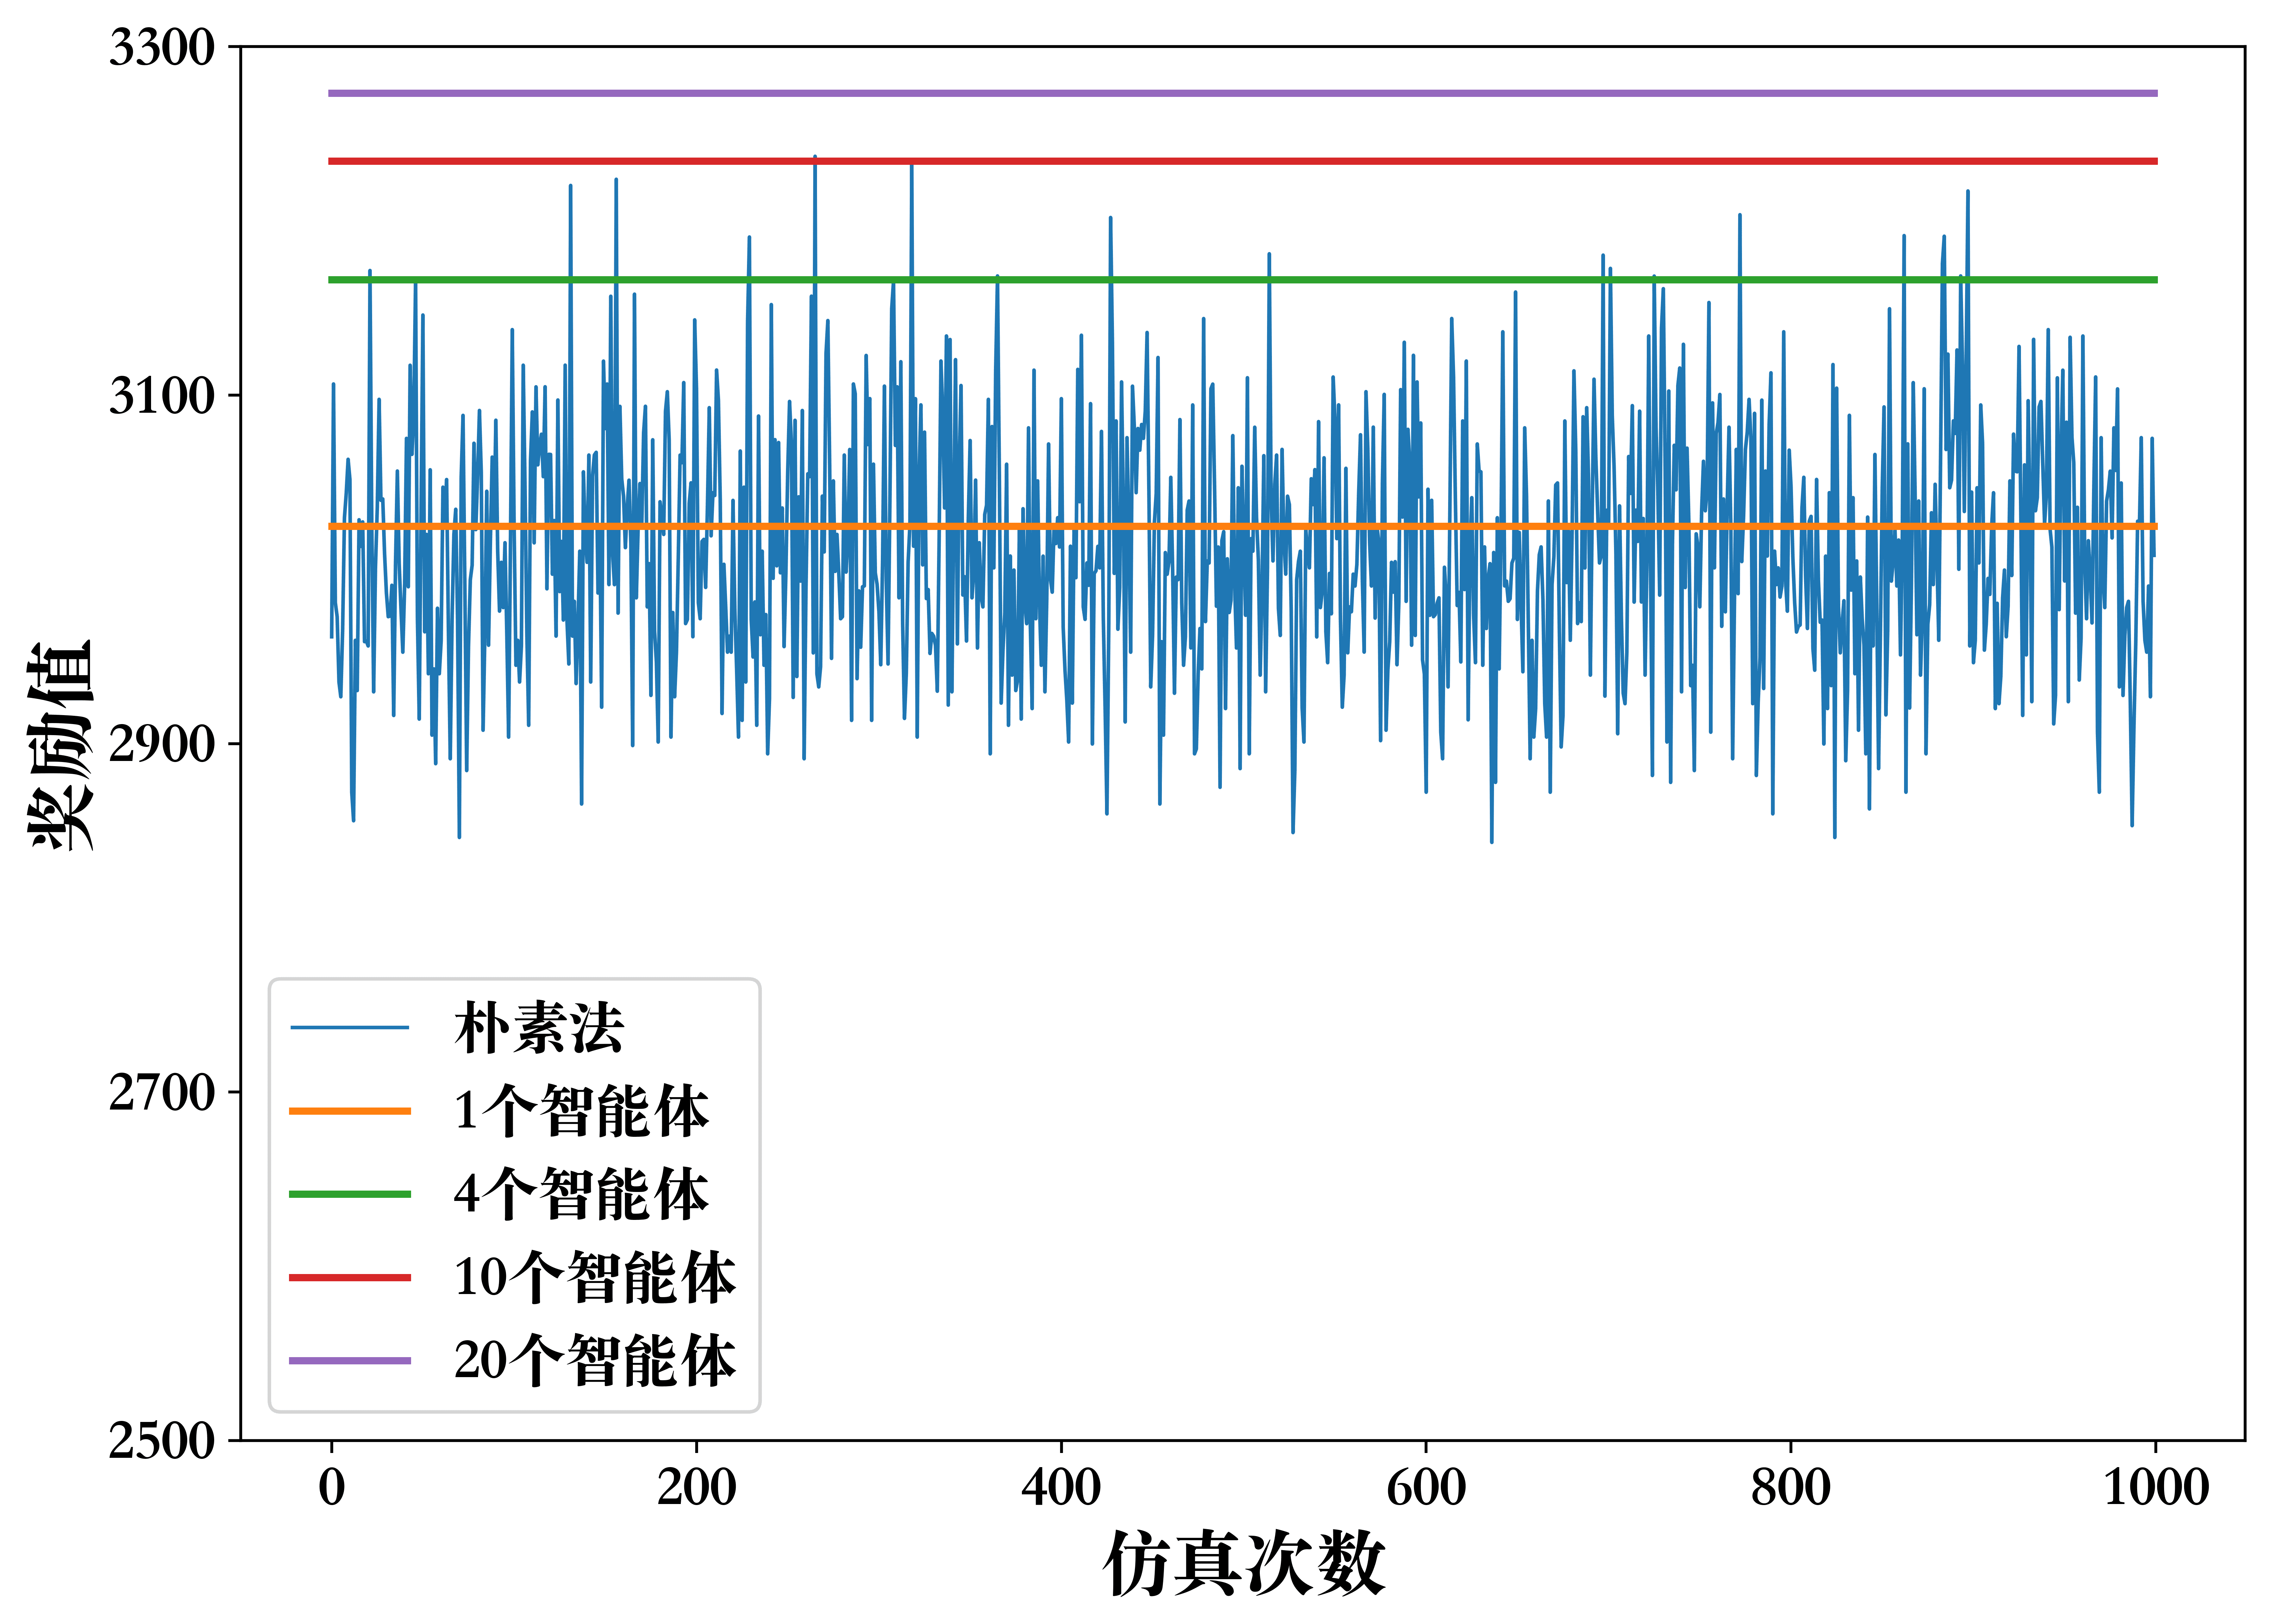
\includegraphics[width=.45\textwidth]{figures/content/size/size5.png}}
  \quad\quad
  \subfloat{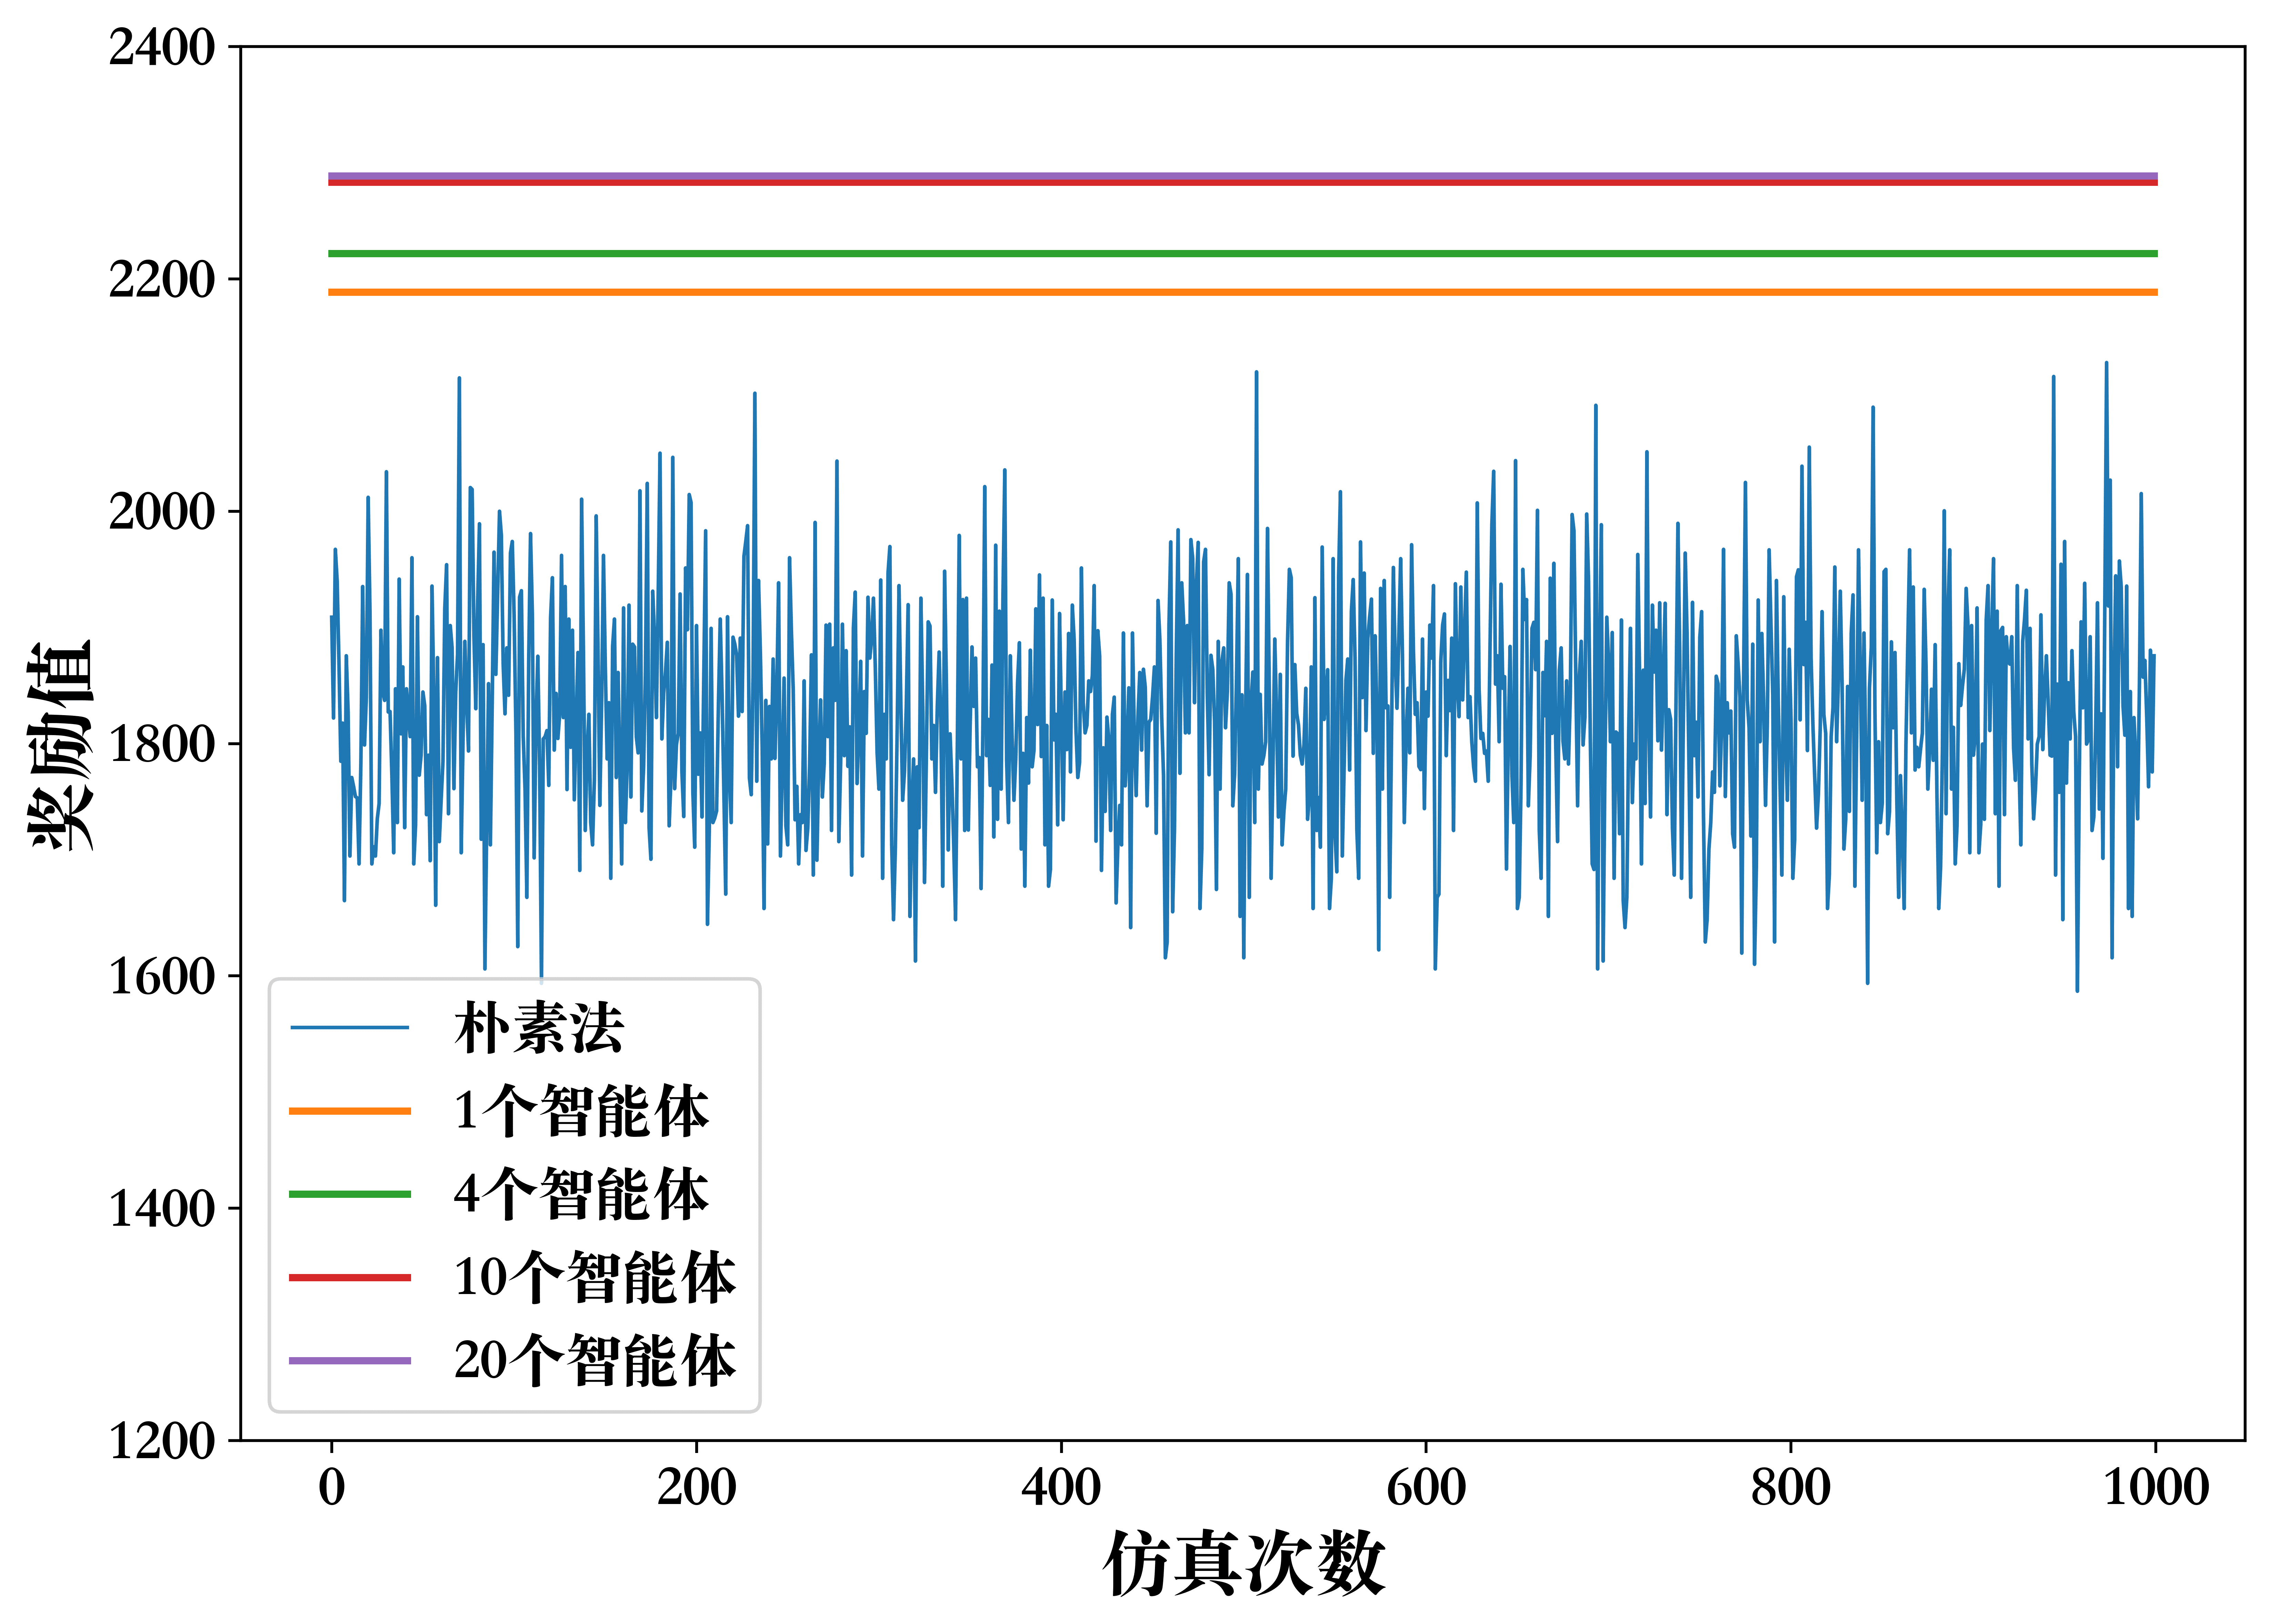
\includegraphics[width=.45\textwidth]{figures/content/size/size6.png}}
  \\
  \subfloat{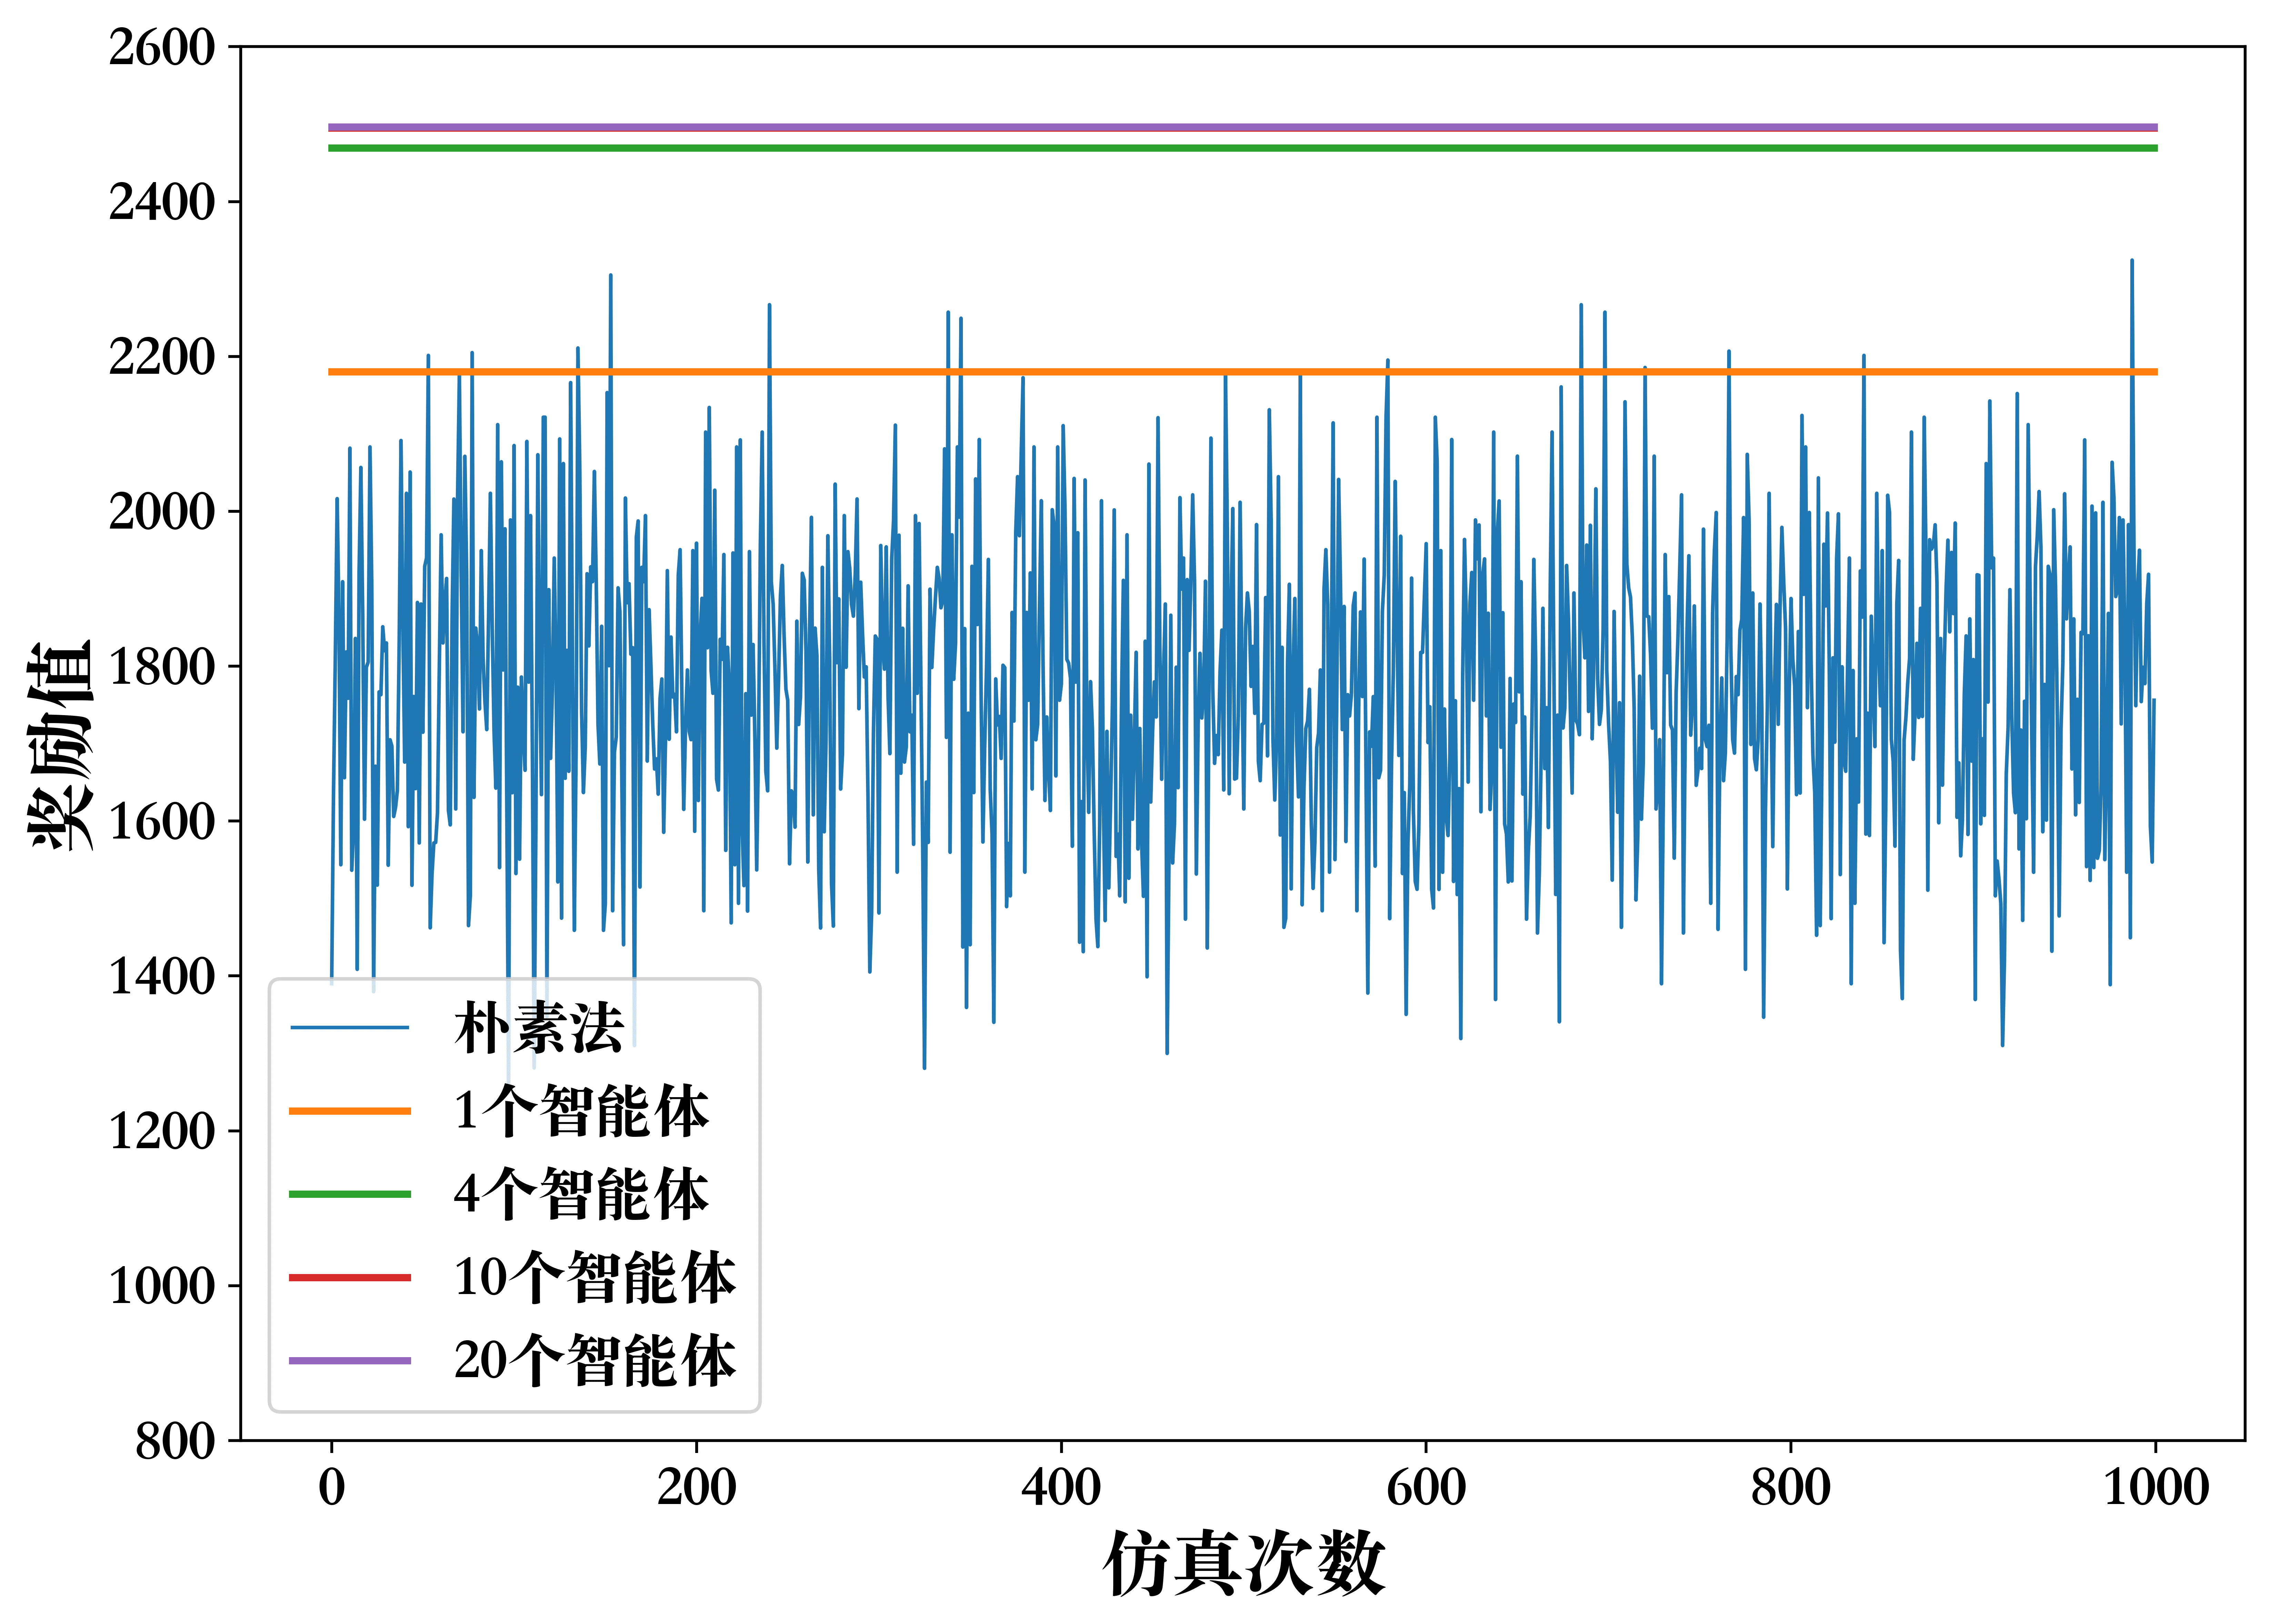
\includegraphics[width=.45\textwidth]{figures/content/size/size7.png}}
  \quad\quad
  \subfloat{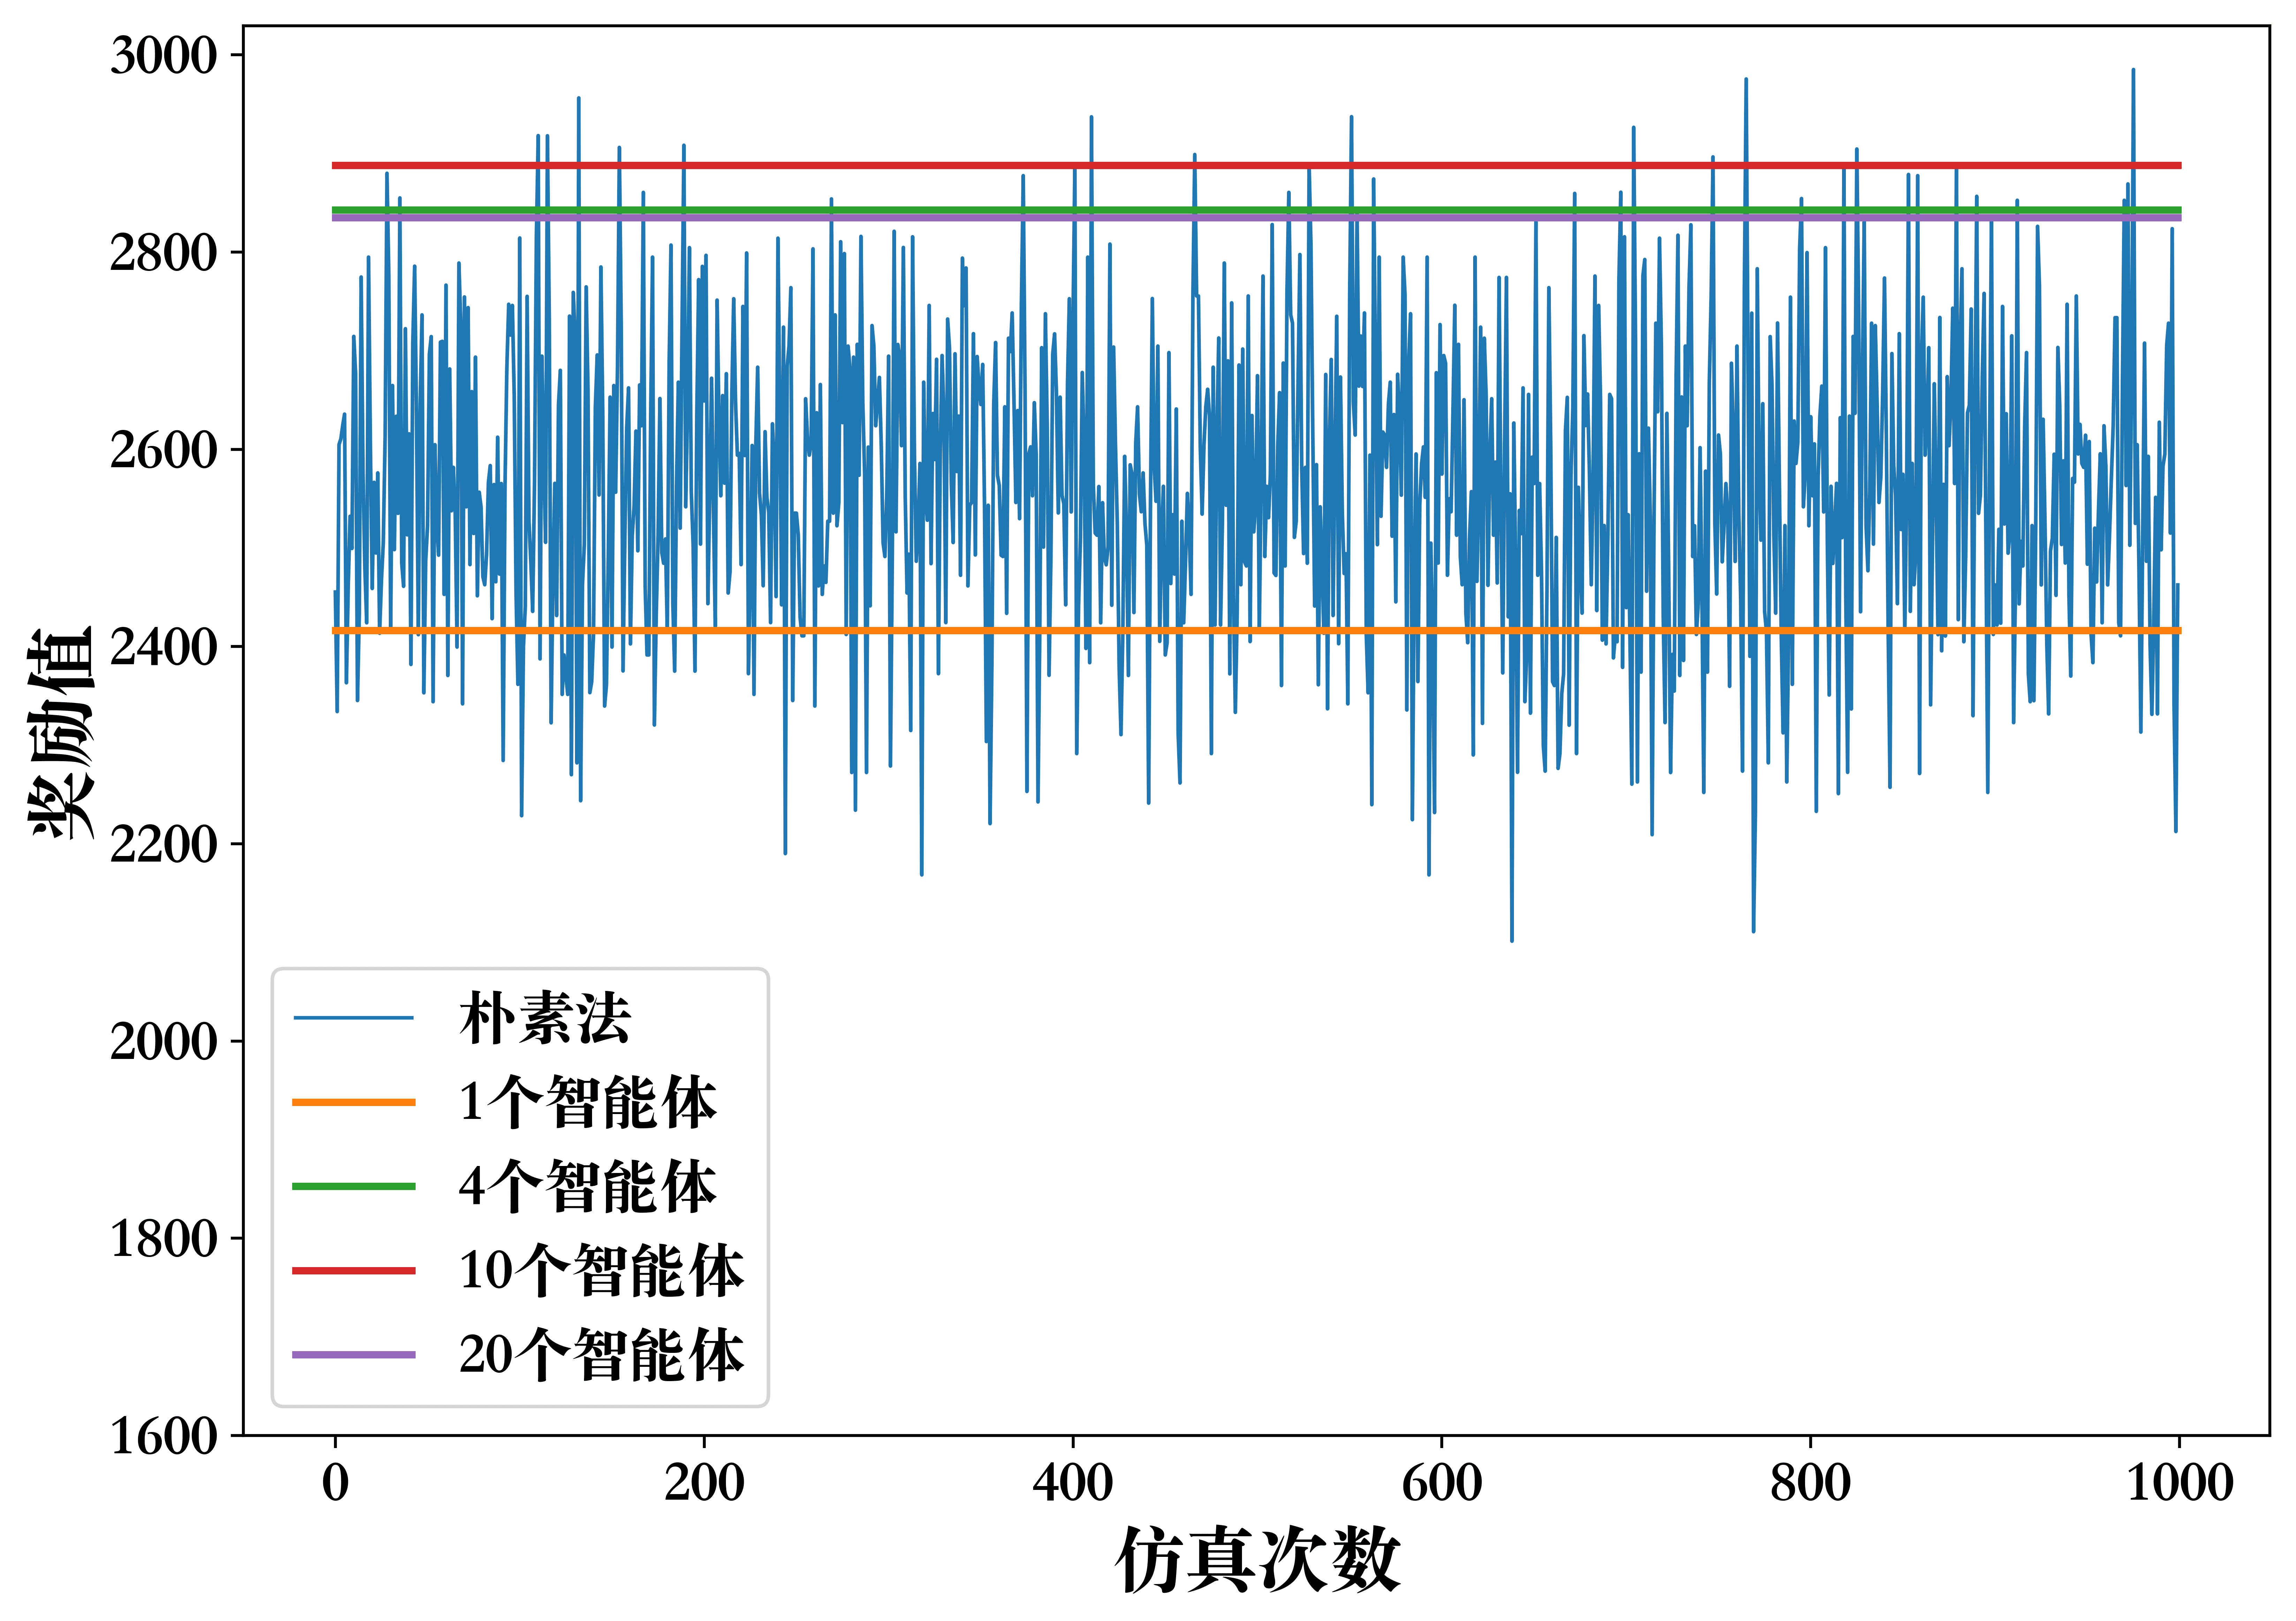
\includegraphics[width=.45\textwidth]{figures/content/size/size8.png}}
  \caption{不同智能体群组训练下的八个测试个体测试结果}
  \label{size}
\end{figure}

\begin{table}[htbp]
\centering
\caption{不同智能体群组训练下所提出方法的性能变化}
\label{cluster_agents}
\renewcommand{\arraystretch}{1.2}
\setlength{\tabcolsep}{6mm}
\small

\begin{tabular}{lccccc}
\toprule
               & 集合1   & 集合2    & 集合3    & 集合4        \\ 
\midrule
平均奖励 & 3,203 & 3,179 & 3,280 & 3,248           \\
超过95\%(共50个)    & 41        & 39         & 43         & 43         \\ 
\bottomrule
\end{tabular}
\end{table}

\begin{figure}[H]
  \centering
  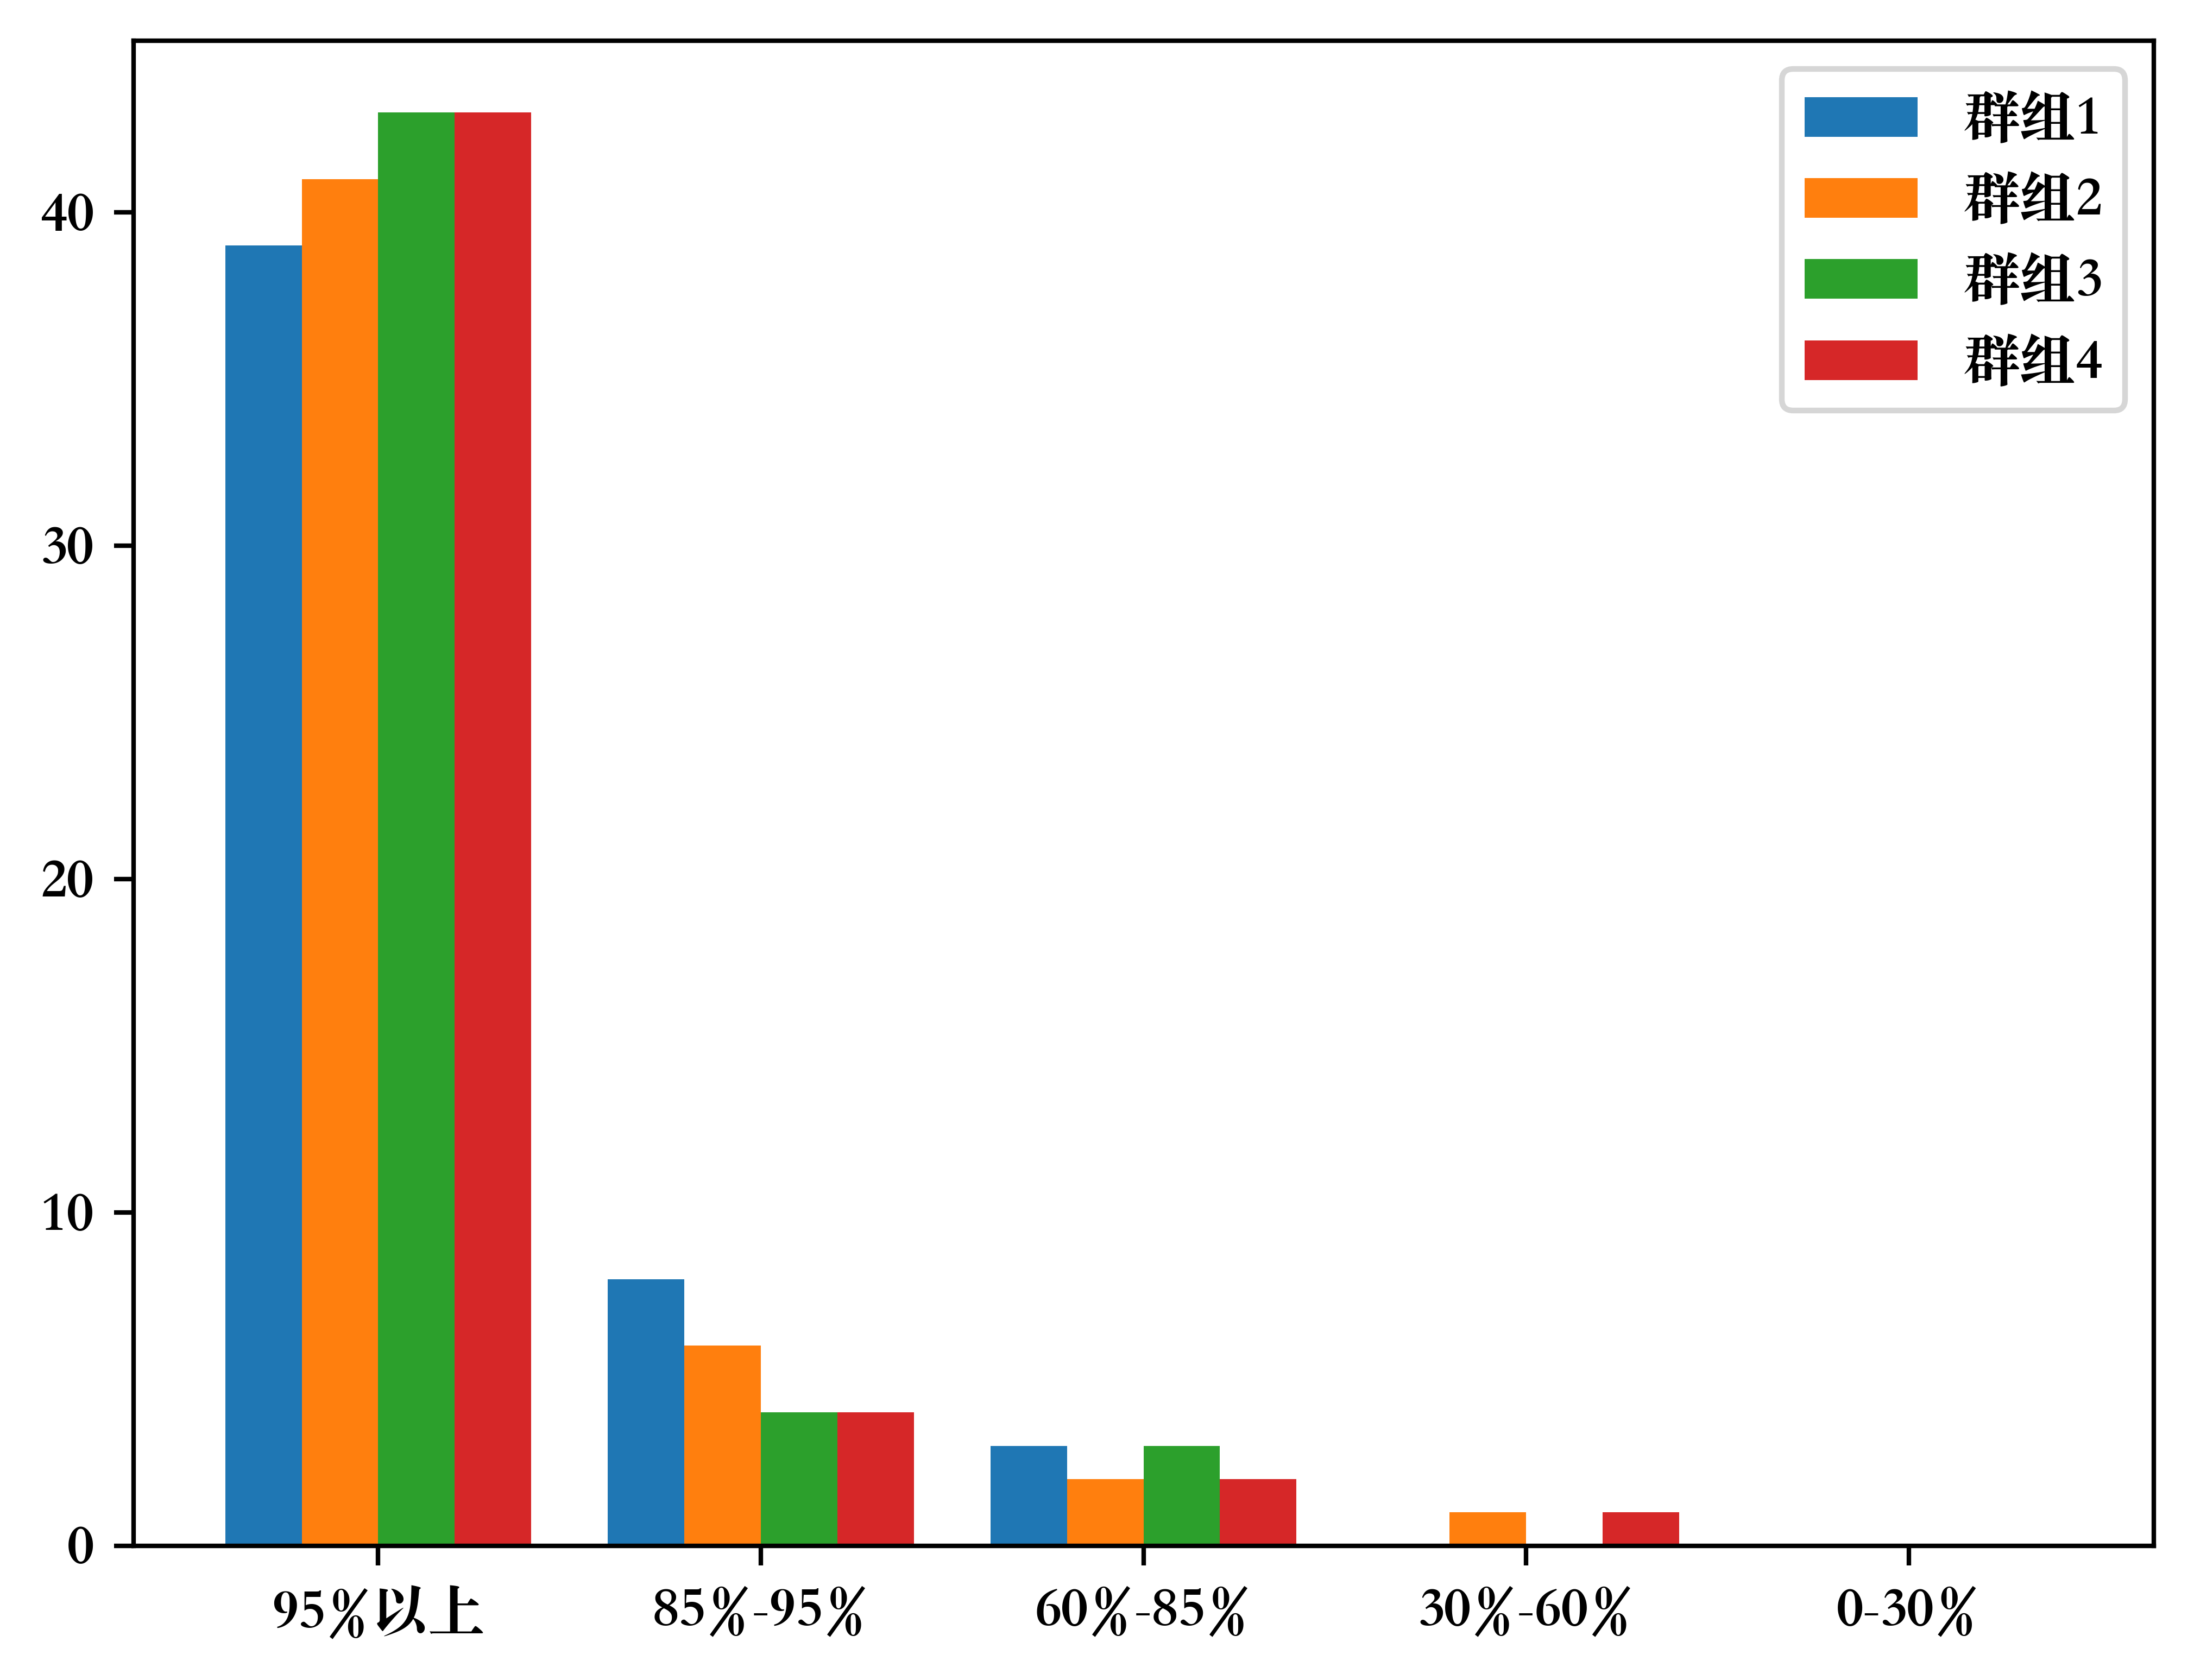
\includegraphics[width=.65\linewidth]{figures/content/set.png}
  \caption{不同智能体群组训练下与朴素法最大奖励值的比较}
  \label{agent_map}
\end{figure}

\section{本章小结}

本章主要介绍了针对所提出的基于深度强化学习方法的训练以及评估。在小节\ref{section:5.1}中介绍了实验场景的设置和智能体的聚类与选取方法,然后详细讨论了模型的训练过程及结果分析,在小节\ref{section:5.2}中对实验结果进行了全面的模型评估,包括与传统DQN方法的对比、各测试个体的性能分析以及模型的泛化能力和灵敏性分析,也包含了模型的最优解、部分信息感知模型检验等多个方面。通过实验得出结论,所提出的基于深度强化学习的模式与出发时间选择方法在交通出行领域中具有很好的应用价值和实际意义。在实验中,该方法在解决许多测试个体的出行模式和出发时间问题时都具有较好的效果,并且相较于传统DQN方法和朴素法,能够更快地收敛到最优解。同时,模型的泛化能力和灵敏性也在一定程度上得到了验证。在未来的研究中,可以进一步优化模型的结构和参数,提高模型的性能和适用范围,以更好地应对实际问题的挑战。
      % 第五章:
\chapter{总结与展望}
\label{chp:version_license}

\section{工作总结}

在现代社会,人们对出行效率和出行体验的要求越来越高,交通问题也日益突出。传统的交通管理方法已经难以应对日益增长的交通需求和不断变化的交通状况。因此,研究如何更好地优化交通流动,提高个体出行效用,是当前交通领域的重要研究方向之一。传统的出行选择模型主要基于随机效用理论,对人们的出行行为进行描述和预测。然而,这些模型忽略了个体对交通环境的实时感知和对环境变化的适应能力,因此其预测准确性有限。而基于深度强化学习的出行选择模型则可以在动态交通环境中实时调整个体的决策策略,提高出行效用,并且具有更高的预测准确性和适应能力。本文提出了一种基于深度强化学习的新型出行模式与时间选择模型,旨在解决传统模型的局限性,并实现更高效、更智能的出行决策。该模型能够适应复杂的交通环境,并且可以处理许多具有出行决策请求的个体,具有较高的计算效率和优秀的性能表现。该研究成果不仅可以为交通管理提供新的思路和方法,还可以为人们提供更高效、更个性化的出行选择建议,提高人们的出行体验和生活质量。论文的主要研究如下:

(1)基于SUMO的城市多模式路网场景

本研究探讨了城市交通多模式仿真环境的建立,主要包括路网编辑与生成、出行模式设计和流量生成三个方面。通过对SUMO搭建仿真路网存在的缺陷和不足进行分析,确保了实验场景能够满足不同研究需求。在出行模式设计部分,考虑了不同交通需求和策略,包括私家车、地铁、公交、自行车等,以便更好地反映城市交通的多样性。在流量生成部分,根据实际数据生成合理的交通流量,提供了准确的交通分析。通过该多模式仿真环境的建立,为交通规划、智慧交通等相关领域的研究和实践提供了可靠的仿真平台。

(2)出行模式与时间选择问题特定的马尔可夫决策过程

马尔可夫决策模型可以充分考虑不同状态之间的转移概率。在出行模式和时间选择问题中,个体每天的状态可能受到多种因素的影响,例如天气、交通状况等,而这些因素的变化可能会影响个体决策。因此,马尔可夫决策模型可以对这些状态进行建模,并考虑它们之间的转移概率,以更好地理解和解决这些问题。其将整个决策过程形式化为一个数学问题,通过定义状态空间、动作空间和奖励函数,马尔可夫决策框架将出行模式和时间选择问题转化为一个数学问题,从而方便进一步的理论研究和算法优化。


(3)基于深度强化学习的出行模式与时间选择模型

为了在处理出行数据时能够更好地提取和泛化特征,以提高模型的准确性和稳定性。本研究使用了基于聚类的深度强化学习方法,该方法使用聚类算法将出行数据集分成不同的子集,然后对每个子集进行深度强化学习模型的训练。这样做的好处是可以在每个子集中学习更具体和相关的特征,从而提高模型的预测能力。此外,该方法还通过改进深度强化学习模型来进一步提高其准确性和稳定性。整个模型的目的是为了能够更好地解决出行模式与时间选择问题,提高个体的出行效用。

(4)针对改进的深度强化学习方法的训练和评估

深度强化学习方法在解决交通出行中的多目标决策问题方面具有很好的应用潜力和实际意义。但是,深度强化学习方法的训练和评估是一个复杂的过程,需要针对实际问题进行合适的实验场景设置、模型参数调优、训练过程监控和结果分析,才能得出具有参考价值的研究成果。训练和评估可以帮助研究者更好地了解模型的性能、泛化能力和灵敏性等方面的特征,以及与其他方法的比较优劣。本研究对实验结果进行了全面的模型评估,包括与传统DQN方法的对比、各测试个体的性能分析以及模型的泛化能力和灵敏性分析。最终,研究得出的结论是基于深度强化学习的模式与出发时间选择方法在交通出行领域中具有很好的应用价值和实际意义,可以更快地收敛到最优解,并且模型的泛化能力和灵敏性得到了验证。


\section{论文创新点}

本文的创新点如下:

(1)联合出行模式和出发时间选择问题建模为连续多天的马尔可夫决策过程,并用深度强化学习模型求解。

传统的出行模式选择和出发时间选择问题通常被视为静态决策问题,即每次出行都是一个单独的决策过程。但实际上,人们的出行决策往往会受到历史决策的影响,因此将这些决策过程建模为连续多天的马尔科夫决策过程模型是更为真实和合理的。深度强化学习是一种强化学习的方法,可以通过让模型自主学习和改进来解决复杂的决策问题。与传统的规则或手动设计模型相比,深度强化学习模型可以更好地适应实际情况和变化,从而提高模型的效果和性能。

(2)提出一种新的深度强化学习方法,利用聚类算法选取代表性个体进行高效训练,作为解决算法。

本研究提出的基于深度强化学习方法是为了解决多模式出行模式和出发时间选择问题而设计的,而传统的深度强化学习方法的训练过程通常需要大量的训练数据和计算资源。因此,本研究引入了一种新的深度强化学习方法,该方法使用聚类算法对大量个体进行聚类,并从每个聚类中选取代表性个体进行训练。这种方法可以大大减少训练数据和计算资源的需求,提高了训练效率和训练效果。这是本研究提出的一项创新点,也是本研究能够成功解决多模式出行模式和出发时间选择问题的关键因素之一。

(3)在真实城市交通网络上进行多模式微观仿真实验,以展示与验证所提出的方法的有效性。

在交通规划和智能交通领域,很多方法和算法都是基于理论或简化的仿真场景进行设计和验证的。然而,在真实世界的城市网络中,存在许多复杂的因素,如道路拓扑结构、交通信号控制、出行行为等等,这些因素对交通流和出行模式的产生和变化都具有重要的影响。因此,对于交通领域的研究来说,在真实世界网络上进行多模式微观仿真实验是非常重要的,可以更准确地反映出真实的交通情况,并验证所提出的方法的有效性和可行性。本文在真实世界网络上进行了多模式微观仿真实验,并与其他方法进行比较和敏感性分析,验证了所提出方法的优越性和鲁棒性。

\section{展望}

在这项研究中提出了一种深度强化学习方法,为在高峰时段(早上7点至9点)出行的个体提供更好的出行选择。该方法旨在在考虑不同出行方式的同时,最大程度地减少用户的出行时间和成本。研究结果表明,该方法在提供准确、高效的出行建议方面是有效的。这种方法的一个关键优势是其灵活性,因为奖励函数可以根据不同用户或情况的特定需求和要求进行调整。但由于学术水平和时间精力有限,仍存在一些问题值得进一步思考与完善,主要包括:

(1)当前模型是为单个旅行者出行选择推荐而设计的,并没有考虑多个旅行者对交通系统的潜在影响。当前模型的设计是出于简化模型和降低计算复杂度的考虑,因此只考虑了单个旅行者的出行选择。但是,在实际交通系统中,多个旅行者的出行选择会相互影响,可能会导致交通系统的拥堵或效率低下。因此,未来研究可以考虑将模型扩展到多智能体框架,以考虑多个旅行者对交通系统的潜在影响。这种扩展可以提高模型的现实性和适用性,进一步优化交通系统的性能,并对城市交通规划和管理提供更好的指导和支持。

(2)该研究使用了一天的出行需求数据作为输入,以提供第二天的出行建议。这意味着该模型无法提供实时的推荐决策,因为需要等待一天的数据输入。未来的研究可以探索如何整合实时数据以建立实时推荐系统,以便在实时交通拥堵或其他情况下,及时为旅客提供最优的出行建议。这可以通过结合实时交通数据、用户实时出行意向以及其他相关信息来实现。

(3)未来研究可以探索如何将个体的行为和社会人口特征纳入到建模框架中,并考虑将换乘作为一种附加的交通方式纳入到决策过程中。同时,需要研究如何在出行选择方面考虑个体之间的动态互动和合作,以提高整个系统的效率和利用交通网络资源。      % 第六章:

%% ----------------------------------------------------------------------------
%%            Acknowledgement, Appendix, Bibliography and Resume
%% ----------------------------------------------------------------------------
\acknowledgement
感谢许元和樊智猛等前人的工作,没有他们的工作也就不会有这个模板的诞生。也感谢使用该模板的每一个人,因为你们的开放与进取心使得 \LaTeX 在东南大学的氛围越来越好。    % 致谢
\thesisbib{reference}               % 生成参考文献

%% 下面一句只是用于提示 TexPad 参考文献位置,正式生成时一定要删除
%\bibliography{reference.bib} % 告诉编译器参考文献所在文件

%\appendix
\newtheorem{theorem}{定理}

\chapter{欧几里得第二定理的证明}
\label{appendix:apps}

	\begin{theorem}
		欧几里得第二定理(素数有无穷多个)\\
		证明:用反证法。假设素数有有限个($N$个),记为$p_1,p_2,\dots,p_N$。则我们构造一个新的数,
		
		\[n=p_1p_2\dots p_N+1.\]
		
		由于$p_i,i=1,2,\dots,N$为素数,则一定不为$1$。于是对于任意的$p_i,i=1,2,\dots, N$,有
		
		\[p_i\not|n\]
		
		这表明,要么$n$本身为素数,要么$n$为合数,但是存在$p_1,p_2,\dots,p_N$之外的其他素数能够将$n$进行素因子分解。不管哪种情况,都表明存在更多的素数。定理得证。\qed
	\end{theorem}

\chapter{$\sqrt{2}$是无理数的证明}
	\begin{theorem}
		$\sqrt{2}$是无理数。\\
		证明:用反证法。假设$\sqrt{2}$是有理数,则可表示为两个整数的商,即$\exists p,q, q\ne0$
		
		\[\sqrt{2}=\frac{p}{q}\]
		
		不失一般性,我们假设$p,q$是既约的,即$\gcd(p,q)=1$。对上式两边平方可得\\
		
		\begin{align*}
			2& =\frac{p^2}{q^2}\\
			p^2&=2q^2.
		\end{align*}
		
		表明$p^2$为偶数,因此$p$为偶数,记$p=2m$。则
		
		\begin{align*}
			p^2&=4m^2=2q^2\\
			q^2&=2m^2.
		\end{align*}
		
		表明$q$也为偶数,因此它们有公共因子$2$。这与它们既约的假设矛盾。定理得证。\qed
	\end{theorem}            % 附录
\resume{作者简介}

。。

~~

\begin{flushleft} 
  \bfseries\large 作者攻读硕士学位期间发表的论文\\
  \relax
\end{flushleft}

\begin{enumerate}
  \renewcommand{\labelenumi}{[\theenumi].}
  \item \textbf{ZHi X}, WEI T, CHEN R, et al.   \item \textbf{ZHi X}, WEI T, JI H, et al.  \item 韦天, \textbf{知心哥哥}. 
\end{enumerate}

~~

\begin{flushleft}
  \bfseries\large 作者攻读硕士学位期间参与的研究课题\\
  \relax
\end{flushleft}

\begin{enumerate}
  \renewcommand{\labelenumi}{[\theenumi].}
  \item \textbf{2018.5-2019.2}:
  \item \textbf{2020.1-2020.3}:
\end{enumerate}
             % 作者简介

\end{document}
